% Generated by Sphinx.
\def\sphinxdocclass{report}
\documentclass[letterpaper,11pt,english]{sphinxmanual}
\usepackage[utf8]{inputenc}
\DeclareUnicodeCharacter{00A0}{\nobreakspace}
\usepackage{cmap}
\usepackage[T1]{fontenc}
\usepackage{babel}
\usepackage{times}
\usepackage[Bjarne]{fncychap}
\usepackage{longtable}
\usepackage{sphinx}
\usepackage{multirow}
\usepackage{amsmath}
\usepackage{mathtools}
\usepackage{amsfonts}
\usepackage{amssymb}
\usepackage{dsfont}
\def\X{\mathbf{X}}
\def\By{\mathbf{y}}
\def\Bbeta{\boldsymbol{\beta}}


\title{Learning Apache Spark with Python}
\date{September 24, 2017}
\release{v1.0}
\author{Wenqiang Feng}
\newcommand{\sphinxlogo}{
\includegraphics{logo.jpg}\par}
\renewcommand{\releasename}{Release}
\makeindex

\makeatletter
\def\PYG@reset{\let\PYG@it=\relax \let\PYG@bf=\relax%
    \let\PYG@ul=\relax \let\PYG@tc=\relax%
    \let\PYG@bc=\relax \let\PYG@ff=\relax}
\def\PYG@tok#1{\csname PYG@tok@#1\endcsname}
\def\PYG@toks#1+{\ifx\relax#1\empty\else%
    \PYG@tok{#1}\expandafter\PYG@toks\fi}
\def\PYG@do#1{\PYG@bc{\PYG@tc{\PYG@ul{%
    \PYG@it{\PYG@bf{\PYG@ff{#1}}}}}}}
\def\PYG#1#2{\PYG@reset\PYG@toks#1+\relax+\PYG@do{#2}}

\expandafter\def\csname PYG@tok@gd\endcsname{\def\PYG@tc##1{\textcolor[rgb]{0.63,0.00,0.00}{##1}}}
\expandafter\def\csname PYG@tok@gu\endcsname{\let\PYG@bf=\textbf\def\PYG@tc##1{\textcolor[rgb]{0.50,0.00,0.50}{##1}}}
\expandafter\def\csname PYG@tok@gt\endcsname{\def\PYG@tc##1{\textcolor[rgb]{0.00,0.27,0.87}{##1}}}
\expandafter\def\csname PYG@tok@gs\endcsname{\let\PYG@bf=\textbf}
\expandafter\def\csname PYG@tok@gr\endcsname{\def\PYG@tc##1{\textcolor[rgb]{1.00,0.00,0.00}{##1}}}
\expandafter\def\csname PYG@tok@cm\endcsname{\let\PYG@it=\textit\def\PYG@tc##1{\textcolor[rgb]{0.25,0.50,0.56}{##1}}}
\expandafter\def\csname PYG@tok@vg\endcsname{\def\PYG@tc##1{\textcolor[rgb]{0.73,0.38,0.84}{##1}}}
\expandafter\def\csname PYG@tok@m\endcsname{\def\PYG@tc##1{\textcolor[rgb]{0.13,0.50,0.31}{##1}}}
\expandafter\def\csname PYG@tok@mh\endcsname{\def\PYG@tc##1{\textcolor[rgb]{0.13,0.50,0.31}{##1}}}
\expandafter\def\csname PYG@tok@cs\endcsname{\def\PYG@tc##1{\textcolor[rgb]{0.25,0.50,0.56}{##1}}\def\PYG@bc##1{\setlength{\fboxsep}{0pt}\colorbox[rgb]{1.00,0.94,0.94}{\strut ##1}}}
\expandafter\def\csname PYG@tok@ge\endcsname{\let\PYG@it=\textit}
\expandafter\def\csname PYG@tok@vc\endcsname{\def\PYG@tc##1{\textcolor[rgb]{0.73,0.38,0.84}{##1}}}
\expandafter\def\csname PYG@tok@il\endcsname{\def\PYG@tc##1{\textcolor[rgb]{0.13,0.50,0.31}{##1}}}
\expandafter\def\csname PYG@tok@go\endcsname{\def\PYG@tc##1{\textcolor[rgb]{0.20,0.20,0.20}{##1}}}
\expandafter\def\csname PYG@tok@cp\endcsname{\def\PYG@tc##1{\textcolor[rgb]{0.00,0.44,0.13}{##1}}}
\expandafter\def\csname PYG@tok@gi\endcsname{\def\PYG@tc##1{\textcolor[rgb]{0.00,0.63,0.00}{##1}}}
\expandafter\def\csname PYG@tok@gh\endcsname{\let\PYG@bf=\textbf\def\PYG@tc##1{\textcolor[rgb]{0.00,0.00,0.50}{##1}}}
\expandafter\def\csname PYG@tok@ni\endcsname{\let\PYG@bf=\textbf\def\PYG@tc##1{\textcolor[rgb]{0.84,0.33,0.22}{##1}}}
\expandafter\def\csname PYG@tok@nl\endcsname{\let\PYG@bf=\textbf\def\PYG@tc##1{\textcolor[rgb]{0.00,0.13,0.44}{##1}}}
\expandafter\def\csname PYG@tok@nn\endcsname{\let\PYG@bf=\textbf\def\PYG@tc##1{\textcolor[rgb]{0.05,0.52,0.71}{##1}}}
\expandafter\def\csname PYG@tok@no\endcsname{\def\PYG@tc##1{\textcolor[rgb]{0.38,0.68,0.84}{##1}}}
\expandafter\def\csname PYG@tok@na\endcsname{\def\PYG@tc##1{\textcolor[rgb]{0.25,0.44,0.63}{##1}}}
\expandafter\def\csname PYG@tok@nb\endcsname{\def\PYG@tc##1{\textcolor[rgb]{0.00,0.44,0.13}{##1}}}
\expandafter\def\csname PYG@tok@nc\endcsname{\let\PYG@bf=\textbf\def\PYG@tc##1{\textcolor[rgb]{0.05,0.52,0.71}{##1}}}
\expandafter\def\csname PYG@tok@nd\endcsname{\let\PYG@bf=\textbf\def\PYG@tc##1{\textcolor[rgb]{0.33,0.33,0.33}{##1}}}
\expandafter\def\csname PYG@tok@ne\endcsname{\def\PYG@tc##1{\textcolor[rgb]{0.00,0.44,0.13}{##1}}}
\expandafter\def\csname PYG@tok@nf\endcsname{\def\PYG@tc##1{\textcolor[rgb]{0.02,0.16,0.49}{##1}}}
\expandafter\def\csname PYG@tok@si\endcsname{\let\PYG@it=\textit\def\PYG@tc##1{\textcolor[rgb]{0.44,0.63,0.82}{##1}}}
\expandafter\def\csname PYG@tok@s2\endcsname{\def\PYG@tc##1{\textcolor[rgb]{0.25,0.44,0.63}{##1}}}
\expandafter\def\csname PYG@tok@vi\endcsname{\def\PYG@tc##1{\textcolor[rgb]{0.73,0.38,0.84}{##1}}}
\expandafter\def\csname PYG@tok@nt\endcsname{\let\PYG@bf=\textbf\def\PYG@tc##1{\textcolor[rgb]{0.02,0.16,0.45}{##1}}}
\expandafter\def\csname PYG@tok@nv\endcsname{\def\PYG@tc##1{\textcolor[rgb]{0.73,0.38,0.84}{##1}}}
\expandafter\def\csname PYG@tok@s1\endcsname{\def\PYG@tc##1{\textcolor[rgb]{0.25,0.44,0.63}{##1}}}
\expandafter\def\csname PYG@tok@gp\endcsname{\let\PYG@bf=\textbf\def\PYG@tc##1{\textcolor[rgb]{0.78,0.36,0.04}{##1}}}
\expandafter\def\csname PYG@tok@sh\endcsname{\def\PYG@tc##1{\textcolor[rgb]{0.25,0.44,0.63}{##1}}}
\expandafter\def\csname PYG@tok@ow\endcsname{\let\PYG@bf=\textbf\def\PYG@tc##1{\textcolor[rgb]{0.00,0.44,0.13}{##1}}}
\expandafter\def\csname PYG@tok@sx\endcsname{\def\PYG@tc##1{\textcolor[rgb]{0.78,0.36,0.04}{##1}}}
\expandafter\def\csname PYG@tok@bp\endcsname{\def\PYG@tc##1{\textcolor[rgb]{0.00,0.44,0.13}{##1}}}
\expandafter\def\csname PYG@tok@c1\endcsname{\let\PYG@it=\textit\def\PYG@tc##1{\textcolor[rgb]{0.25,0.50,0.56}{##1}}}
\expandafter\def\csname PYG@tok@kc\endcsname{\let\PYG@bf=\textbf\def\PYG@tc##1{\textcolor[rgb]{0.00,0.44,0.13}{##1}}}
\expandafter\def\csname PYG@tok@c\endcsname{\let\PYG@it=\textit\def\PYG@tc##1{\textcolor[rgb]{0.25,0.50,0.56}{##1}}}
\expandafter\def\csname PYG@tok@mf\endcsname{\def\PYG@tc##1{\textcolor[rgb]{0.13,0.50,0.31}{##1}}}
\expandafter\def\csname PYG@tok@err\endcsname{\def\PYG@bc##1{\setlength{\fboxsep}{0pt}\fcolorbox[rgb]{1.00,0.00,0.00}{1,1,1}{\strut ##1}}}
\expandafter\def\csname PYG@tok@kd\endcsname{\let\PYG@bf=\textbf\def\PYG@tc##1{\textcolor[rgb]{0.00,0.44,0.13}{##1}}}
\expandafter\def\csname PYG@tok@ss\endcsname{\def\PYG@tc##1{\textcolor[rgb]{0.32,0.47,0.09}{##1}}}
\expandafter\def\csname PYG@tok@sr\endcsname{\def\PYG@tc##1{\textcolor[rgb]{0.14,0.33,0.53}{##1}}}
\expandafter\def\csname PYG@tok@mo\endcsname{\def\PYG@tc##1{\textcolor[rgb]{0.13,0.50,0.31}{##1}}}
\expandafter\def\csname PYG@tok@mi\endcsname{\def\PYG@tc##1{\textcolor[rgb]{0.13,0.50,0.31}{##1}}}
\expandafter\def\csname PYG@tok@kn\endcsname{\let\PYG@bf=\textbf\def\PYG@tc##1{\textcolor[rgb]{0.00,0.44,0.13}{##1}}}
\expandafter\def\csname PYG@tok@o\endcsname{\def\PYG@tc##1{\textcolor[rgb]{0.40,0.40,0.40}{##1}}}
\expandafter\def\csname PYG@tok@kr\endcsname{\let\PYG@bf=\textbf\def\PYG@tc##1{\textcolor[rgb]{0.00,0.44,0.13}{##1}}}
\expandafter\def\csname PYG@tok@s\endcsname{\def\PYG@tc##1{\textcolor[rgb]{0.25,0.44,0.63}{##1}}}
\expandafter\def\csname PYG@tok@kp\endcsname{\def\PYG@tc##1{\textcolor[rgb]{0.00,0.44,0.13}{##1}}}
\expandafter\def\csname PYG@tok@w\endcsname{\def\PYG@tc##1{\textcolor[rgb]{0.73,0.73,0.73}{##1}}}
\expandafter\def\csname PYG@tok@kt\endcsname{\def\PYG@tc##1{\textcolor[rgb]{0.56,0.13,0.00}{##1}}}
\expandafter\def\csname PYG@tok@sc\endcsname{\def\PYG@tc##1{\textcolor[rgb]{0.25,0.44,0.63}{##1}}}
\expandafter\def\csname PYG@tok@sb\endcsname{\def\PYG@tc##1{\textcolor[rgb]{0.25,0.44,0.63}{##1}}}
\expandafter\def\csname PYG@tok@k\endcsname{\let\PYG@bf=\textbf\def\PYG@tc##1{\textcolor[rgb]{0.00,0.44,0.13}{##1}}}
\expandafter\def\csname PYG@tok@se\endcsname{\let\PYG@bf=\textbf\def\PYG@tc##1{\textcolor[rgb]{0.25,0.44,0.63}{##1}}}
\expandafter\def\csname PYG@tok@sd\endcsname{\let\PYG@it=\textit\def\PYG@tc##1{\textcolor[rgb]{0.25,0.44,0.63}{##1}}}

\def\PYGZbs{\char`\\}
\def\PYGZus{\char`\_}
\def\PYGZob{\char`\{}
\def\PYGZcb{\char`\}}
\def\PYGZca{\char`\^}
\def\PYGZam{\char`\&}
\def\PYGZlt{\char`\<}
\def\PYGZgt{\char`\>}
\def\PYGZsh{\char`\#}
\def\PYGZpc{\char`\%}
\def\PYGZdl{\char`\$}
\def\PYGZhy{\char`\-}
\def\PYGZsq{\char`\'}
\def\PYGZdq{\char`\"}
\def\PYGZti{\char`\~}
% for compatibility with earlier versions
\def\PYGZat{@}
\def\PYGZlb{[}
\def\PYGZrb{]}
\makeatother

\begin{document}

\maketitle
\tableofcontents
\phantomsection\label{index::doc}\phantomsection\label{index:index}\begin{quote}
\begin{figure}[htbp]
\centering


\includegraphics{logo.jpg}
\label{index:fig-logo}\end{figure}
\end{quote}

Welcome to our \textbf{Learning Apache Spark with Python} note!
In these note, you will learn a wide array of concepts about
\textbf{PySpark} in Data Mining, Text Mining, Machine Leanring
and Deep Learning.




\chapter{Preface}
\label{preface:id1}\label{preface::doc}\label{preface:contents}\label{preface:preface}

\section{About}
\label{preface:about}

\subsection{About this note}
\label{preface:about-this-note}
This is a shared repository for Learning Apache Spark Notes.
The first version was posted on Github in {\hyperref[reference:feng2017]{{[}Feng2017{]}}}.
This shared repository mainly contains the self-learning and
self-teaching notes from Wenqiang during his \href{https://www.ima.umn.edu/2016-2017/SW1.23-3.10.17\#}{IMA Data Science
Fellowship}.

In this repository, I try to use the detailed demo code and
examples to show how to use each main functions. If you find
your work wasn’t cited in this note, please feel free to let
me know.

Although I am by no means an data mining programming and Big Data expert,
I decided that it would be useful for me to share what I learned
about PySpark programming in the form of easy tutorials with
detailed example. I hope those tutorials will be a valuable tool
for your studies.

The tutorials assume that the reader has a preliminary knowledge
of programing and Linux. And this document is generated automatically
by using \href{http://sphinx.pocoo.org}{sphinx}.


\subsection{About the authors}
\label{preface:about-the-authors}\begin{itemize}
\item {} 
\textbf{Wenqiang Feng}
\begin{itemize}
\item {} 
Data Scientist and Phd in Mathematics

\item {} 
University of Tennessee at Knoxville

\item {} 
Email: \href{mailto:wfeng1@utk.edu}{wfeng1@utk.edu}

\end{itemize}

\end{itemize}


\section{Motivation for this tutorial}
\label{preface:motivation-for-this-tutorial}
I was motivated by the \href{https://www.ima.umn.edu/2016-2017/SW1.23-3.10.17\#}{IMA Data Science Fellowship}
project to learn PySpark. After that I was impressed and attracted by the
PySpark. And I foud that:
\begin{enumerate}
\item {} 
It is no exaggeration to say that Spark is the most powerful
Bigdata tool.

\item {} 
However, I still found that learning Spark was a difficult
process. I have to Google it and identify which one is true.
And it was hard to find detailed examples which I can easily
learned the full process in one file.

\item {} 
Good sources are expensive for a graduate student.

\end{enumerate}


\section{Acknowledgement}
\label{preface:acknowledgement}
At here, I would like to thank Ming Chen, Jian Sun and Zhongbo Li at the
University of Tennessee at Knoxville for the valuable disscussion
and thank the generous anonymous authors for providing the detailed
solutions and source code on the internet. Without those help,
this repository would not have been possible to be made. Wenqiang
also would like to thank the \href{https://www.ima.umn.edu/}{Institute for Mathematics and Its
Applications (IMA)} at \href{https://twin-cities.umn.edu/}{University of Minnesota, Twin Cities}
for support during his IMA Data Scientist Fellow visit.


\section{Feedback and suggestions}
\label{preface:feedback-and-suggestions}
Your comments and suggestions are highly appreciated. I am more
than happy to receive corrections, suggestions or feedbacks through
email (\href{mailto:wfeng1@utk.edu}{wfeng1@utk.edu}) for improvements.


\chapter{Why Spark with Python ?}
\label{why:university-of-minnesota-twin-cities}\label{why::doc}\label{why:why}\label{why:why-spark-with-python}
\begin{notice}{note}{Note:}
\textbf{Sharpening the knife longer can make it easier to hack the firewood} -- old Chinese proverb
\end{notice}

I want to answer this question from the following two parts:


\section{Why Spark?}
\label{why:why-spark}
I think the following four main reasons form \href{http://spark.apache.org/}{Apache Spark™} official website are good enough
to convince you to use Spark.
\begin{enumerate}
\item {} 
Speed

Run programs up to 100x faster than Hadoop MapReduce in memory, or 10x faster on disk.

Apache Spark has an advanced DAG execution engine that supports acyclic data flow and in-memory computing.

\end{enumerate}
\begin{quote}
\begin{figure}[htbp]
\centering
\capstart

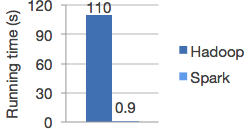
\includegraphics{logistic-regression.png}
\caption{Logistic regression in Hadoop and Spark}\label{why:fig-lr}\end{figure}
\end{quote}
\begin{enumerate}
\setcounter{enumi}{1}
\item {} 
Ease of Use

Write applications quickly in Java, Scala, Python, R.

Spark offers over 80 high-level operators that make it easy to build parallel apps. And you can use it interactively from the Scala, Python and R shells.

\item {} 
Generality

Combine SQL, streaming, and complex analytics.

Spark powers a stack of libraries including SQL and DataFrames, MLlib for machine learning, GraphX, and Spark Streaming. You can combine these libraries seamlessly in the same application.

\end{enumerate}
\begin{quote}
\begin{figure}[htbp]
\centering
\capstart

\scalebox{0.700000}{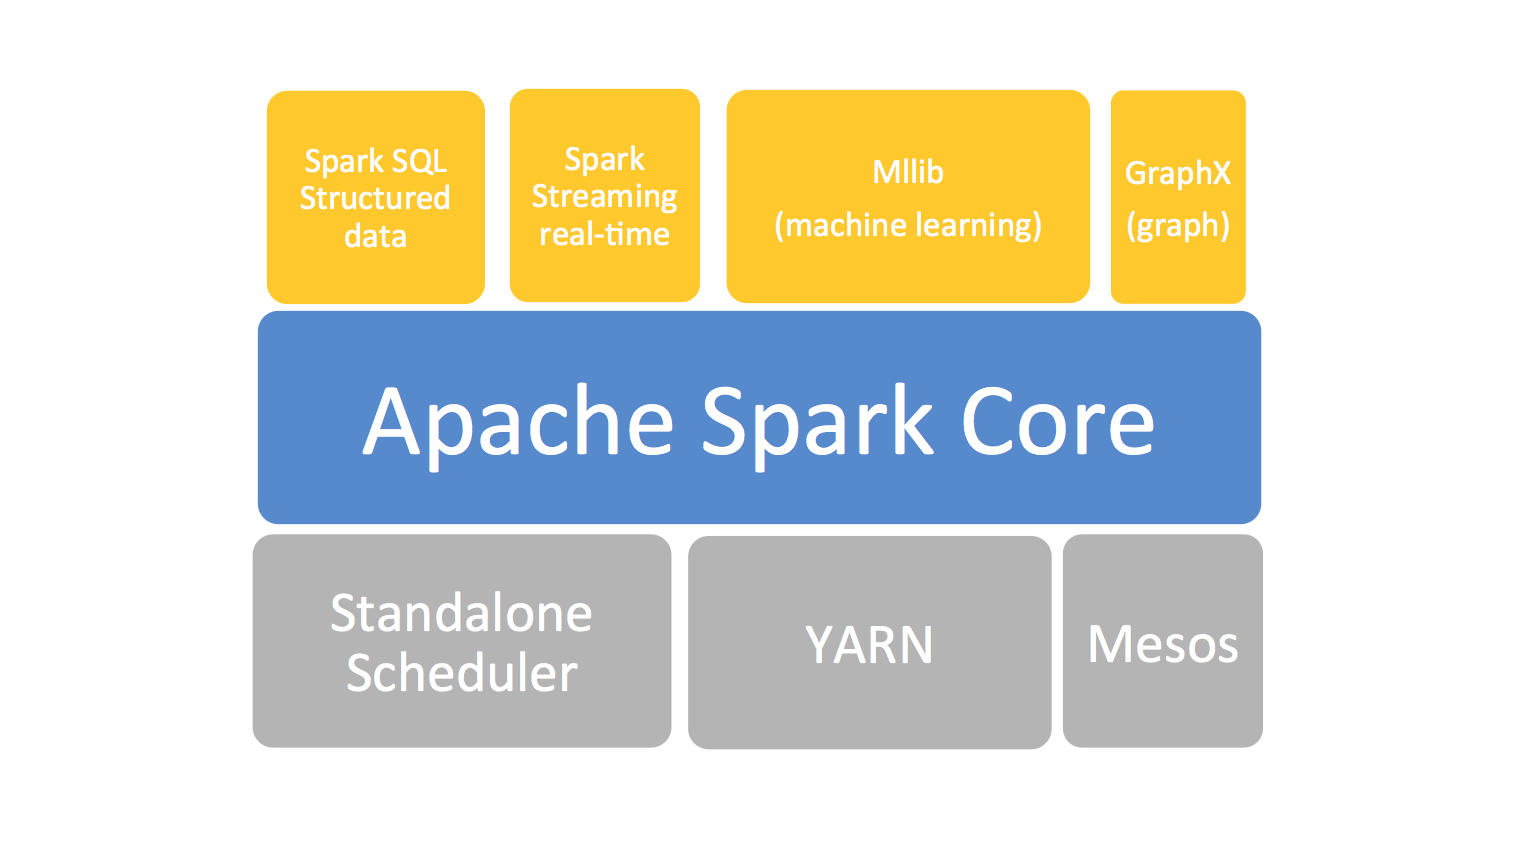
\includegraphics{stack.png}}
\caption{The Spark stack}\label{why:fig-stack}\end{figure}
\end{quote}
\begin{enumerate}
\setcounter{enumi}{3}
\item {} 
Runs Everywhere

Spark runs on Hadoop, Mesos, standalone, or in the cloud. It can access diverse data sources including HDFS, Cassandra, HBase, and S3.

\end{enumerate}
\begin{quote}
\begin{figure}[htbp]
\centering
\capstart

\scalebox{0.600000}{
\includegraphics{spark-runs-everywhere.png}}
\caption{The Spark platform}\label{why:fig-runs}\end{figure}
\end{quote}


\section{Why Spark with Python (PySpark)?}
\label{why:why-spark-with-python-pyspark}
No matter you like it or not, Python has been one of the most popular programming languages.
\begin{quote}
\begin{figure}[htbp]
\centering
\capstart

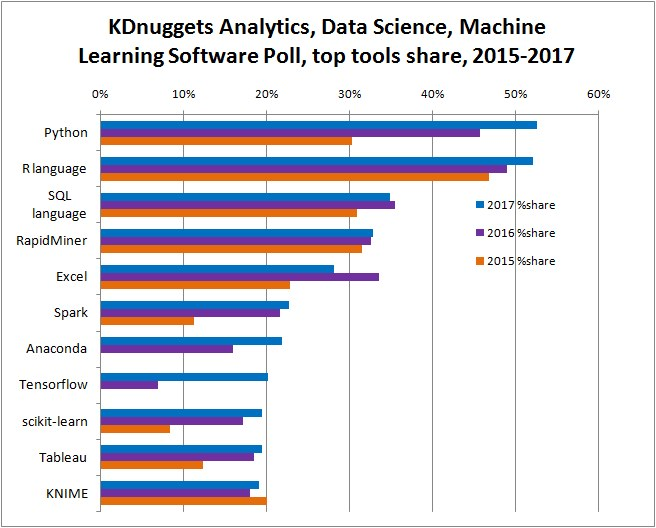
\includegraphics{languages.jpg}
\caption{KDnuggets Analytics/Data Science 2017 Software Poll from \href{http://www.kdnuggets.com/2017/05/poll-analytics-data-science-machine-learning-software-leaders.html}{kdnuggets}.}\label{why:fig-languages}\end{figure}
\end{quote}


\chapter{Configure Running Platform}
\label{setup:configure-running-platform}\label{setup:setup}\label{setup:kdnuggets}\label{setup::doc}
\begin{notice}{note}{Note:}
\textbf{Good tools are prerequisite to the successful execution
of a job.} -- old Chinese proverb
\end{notice}

A good programming platform can save you lots of troubles and time.
Herein I will only present how to install my favorite programming
platform and only show the easiest way which I know to set it up
on Linux system. If you want to install on the other operator
system, you can Google it. In this section, you may learn how to
set up Pyspark on the corresponding programming platform and package.

\index{Run on Databricks Community Cloud}

\section{Run on Databricks Community Cloud}
\label{setup:run-on-databricks-community-cloud}\label{setup:index-0}
If you don't have any experience with Linux or Unix operator
system, I would love to recommend you to use Spark on Databricks
Community Cloud. Since you do not need to setup the Spark and it's
totally \textbf{free} for Community Edition. Please follow the steps
listed below.
\begin{quote}
\begin{enumerate}
\item {} 
Sign up a account at: \href{https://community.cloud.databricks.com/login.html}{https://community.cloud.databricks.com/login.html}

\end{enumerate}
\begin{quote}
\begin{figure}[htbp]
\centering

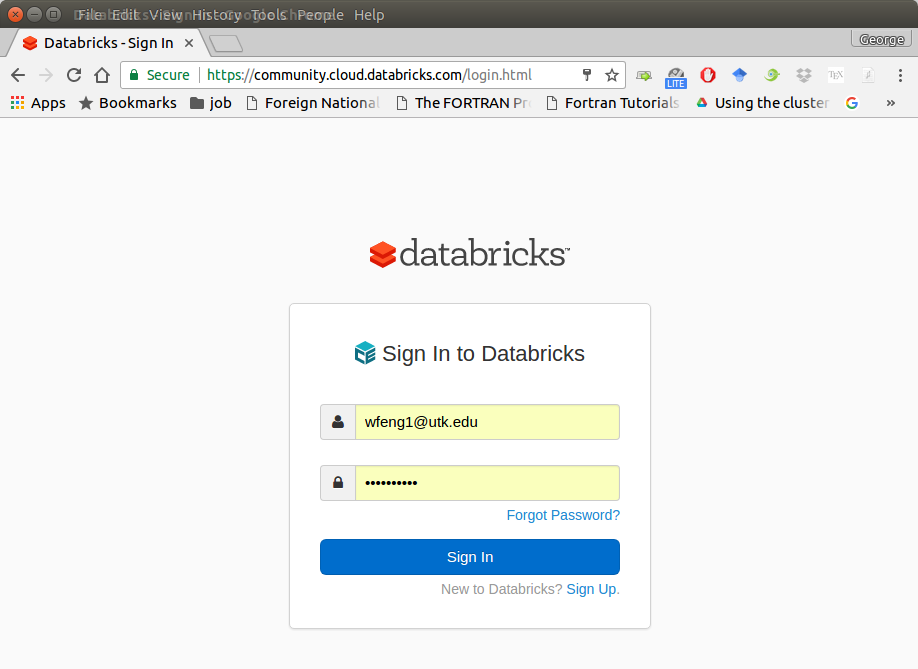
\includegraphics{login.png}
\label{setup:fig-login}\end{figure}
\end{quote}
\begin{enumerate}
\setcounter{enumi}{1}
\item {} 
Sign in with your account, then you can creat your cluster(machine), table(dataset)
and notebook(code).

\end{enumerate}
\begin{quote}
\begin{figure}[htbp]
\centering

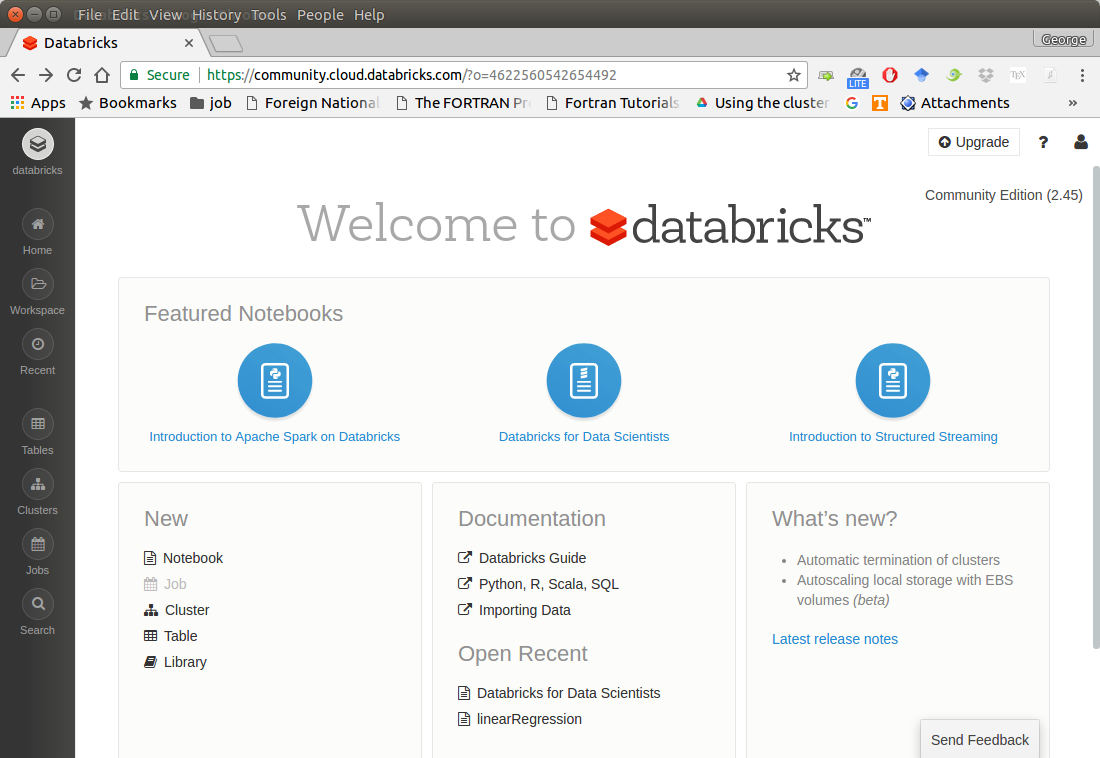
\includegraphics{workspace.png}
\label{setup:fig-workspace}\end{figure}
\end{quote}
\begin{enumerate}
\setcounter{enumi}{2}
\item {} 
Create your cluster where your code will run

\end{enumerate}
\begin{quote}
\begin{figure}[htbp]
\centering

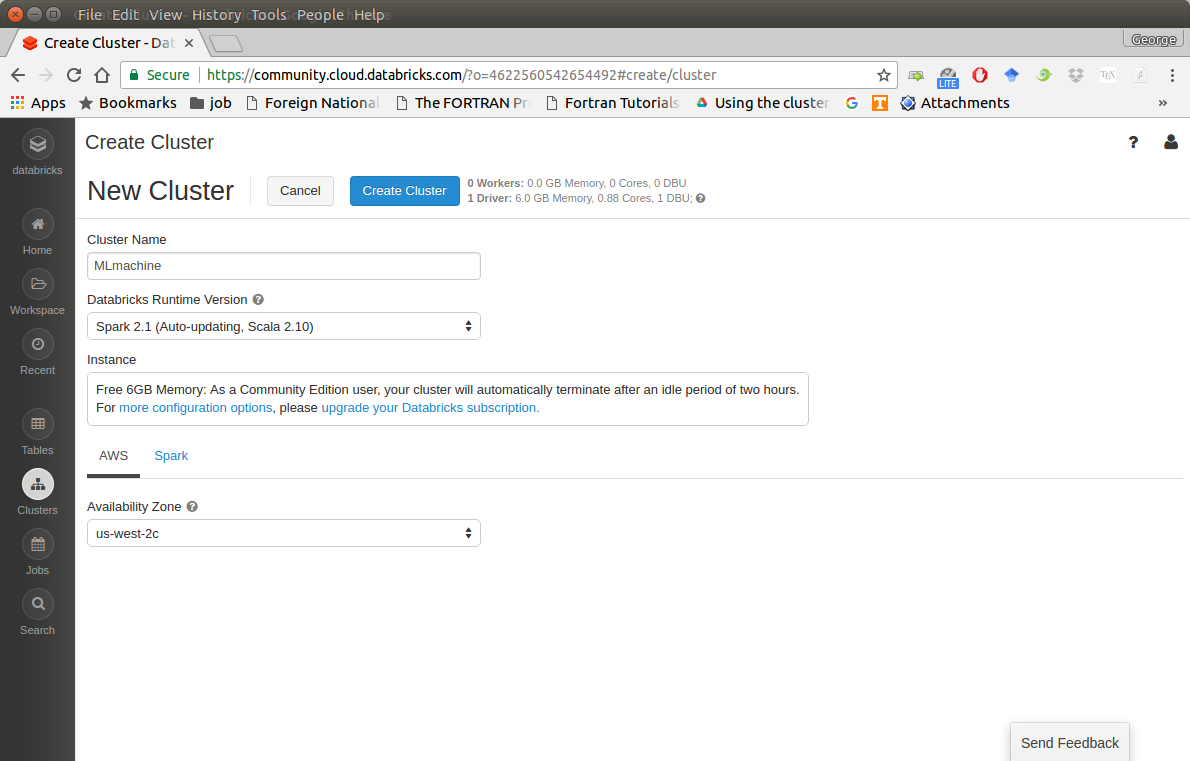
\includegraphics{cluster.png}
\label{setup:fig-cluster}\end{figure}
\end{quote}
\begin{enumerate}
\setcounter{enumi}{3}
\item {} 
Import your dataset

\end{enumerate}
\begin{quote}
\begin{figure}[htbp]
\centering

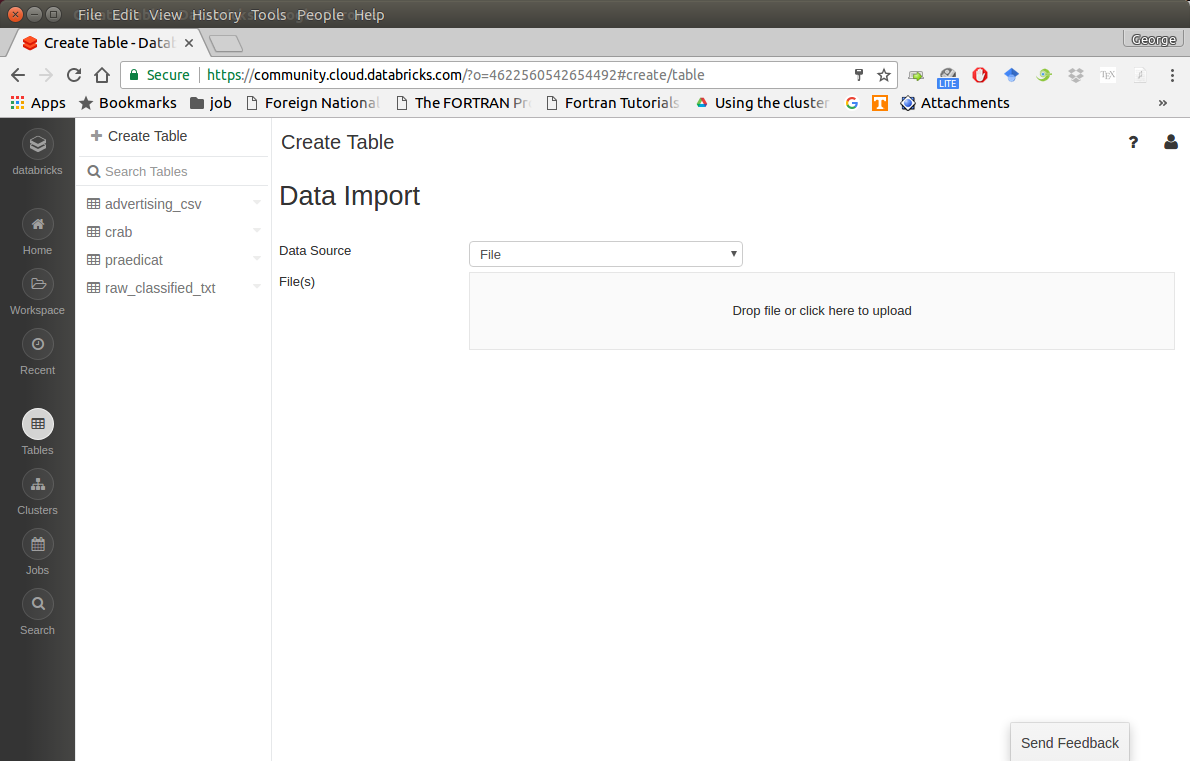
\includegraphics{table.png}
\label{setup:fig-table}\end{figure}
\begin{figure}[htbp]
\centering

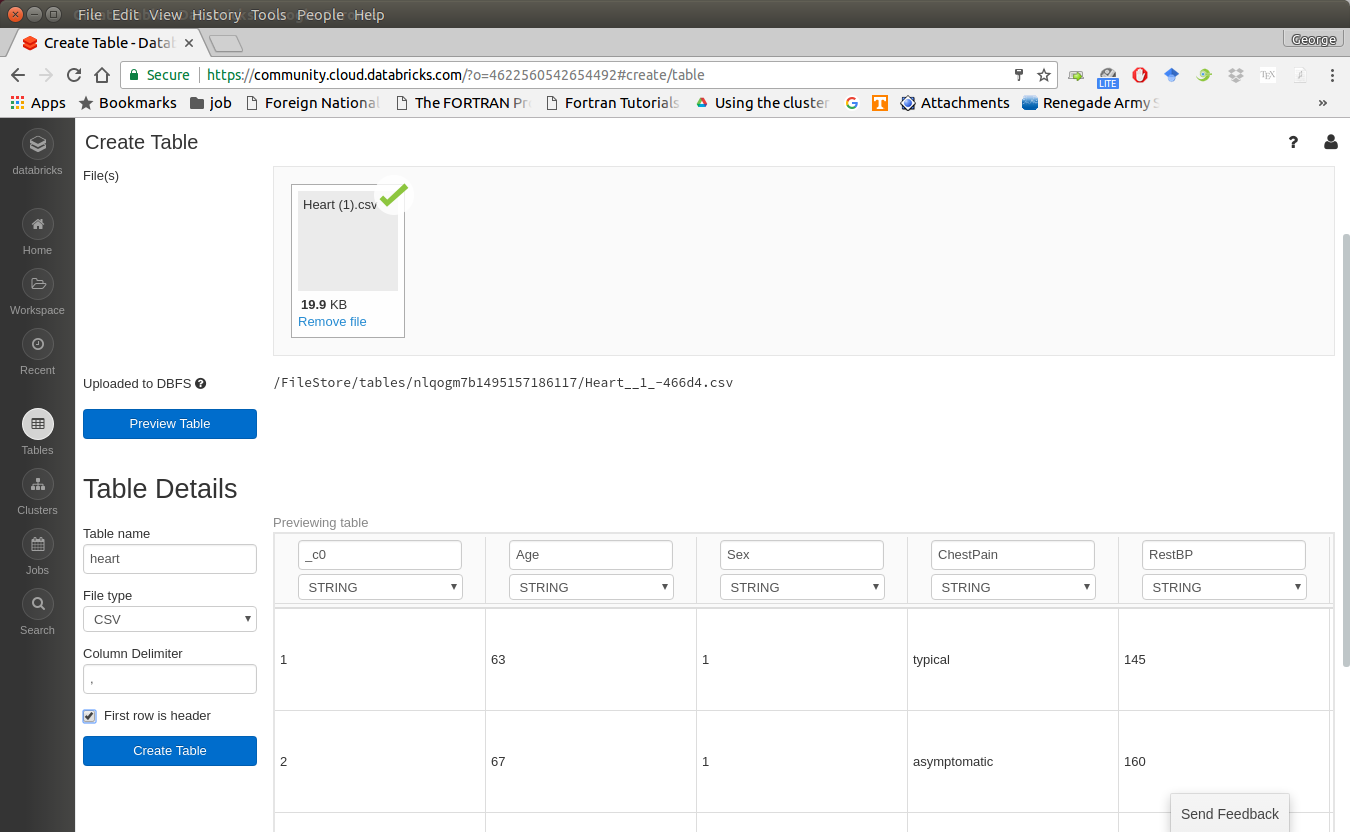
\includegraphics{dataset1.png}
\label{setup:fig-dataset1}\end{figure}
\end{quote}

\begin{notice}{note}{Note:}
You need to save the path which appears at Uploaded to DBFS:
/FileStore/tables/05rmhuqv1489687378010/. Since we will use
this path to load the dataset.
\end{notice}
\end{quote}
\begin{enumerate}
\setcounter{enumi}{4}
\item {} 
Creat your notebook

\end{enumerate}
\begin{quote}
\begin{figure}[htbp]
\centering

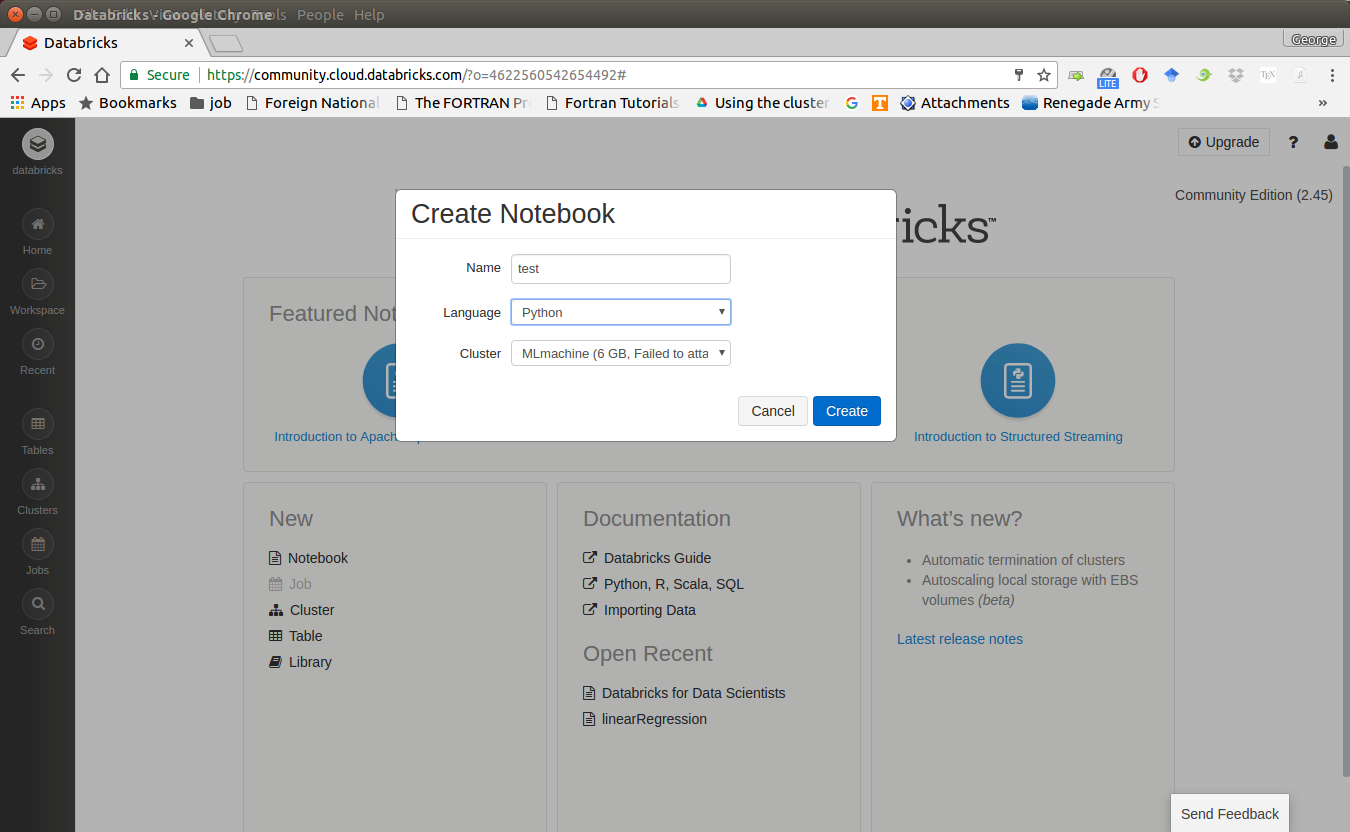
\includegraphics{notebook.png}
\label{setup:fig-notebook}\end{figure}
\begin{figure}[htbp]
\centering

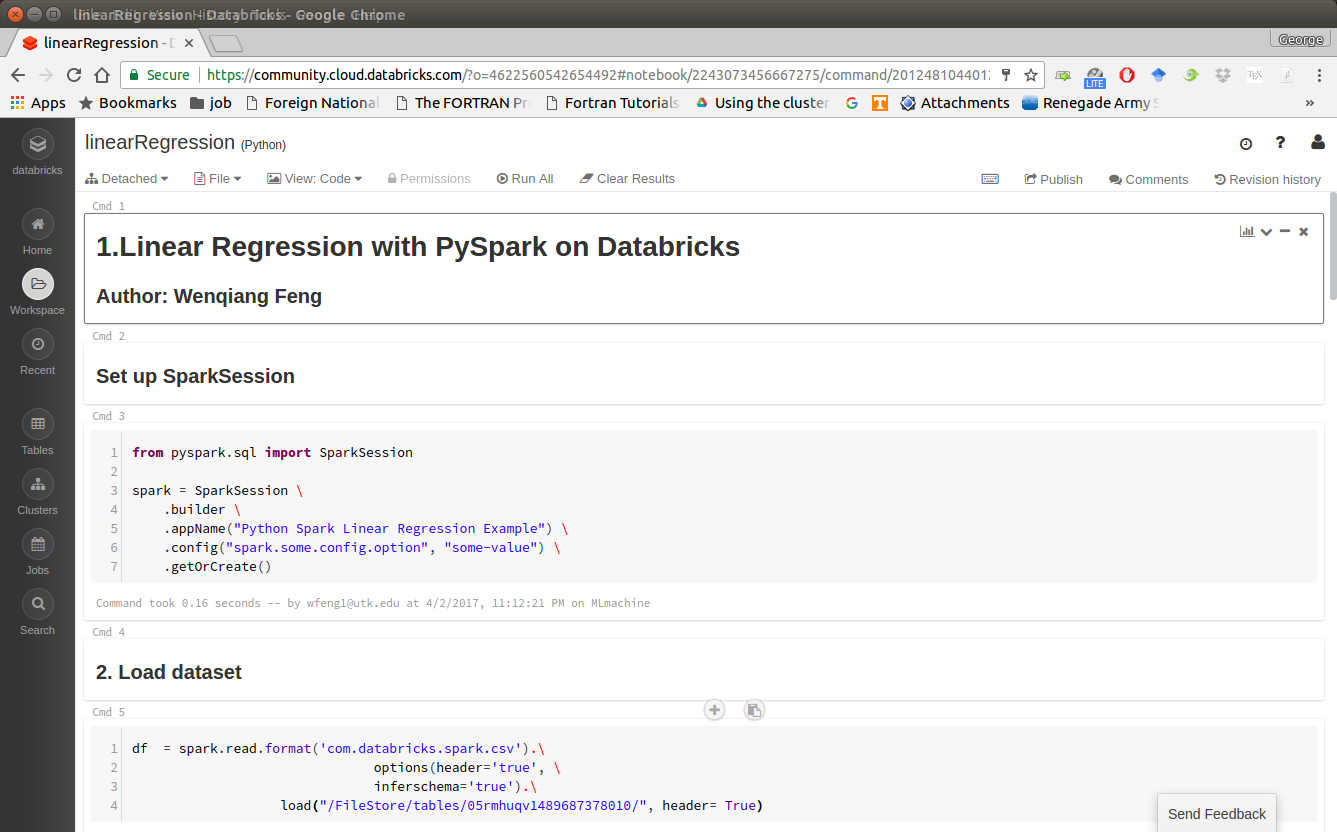
\includegraphics{codenotebook.png}
\label{setup:fig-codenotebook}\end{figure}
\end{quote}

After finishing the above 5 steps, you are ready to run your
Spark code on Databricks Community Cloud. I will run all the
following demos on Databricks Community Cloud. Hopefully, when
you run the demo code, you will get the following results:
\begin{quote}

\begin{Verbatim}[commandchars=\\\{\}]
\PYG{o}{+}\PYG{o}{\PYGZhy{}}\PYG{o}{\PYGZhy{}}\PYG{o}{\PYGZhy{}}\PYG{o}{+}\PYG{o}{\PYGZhy{}}\PYG{o}{\PYGZhy{}}\PYG{o}{\PYGZhy{}}\PYG{o}{\PYGZhy{}}\PYG{o}{\PYGZhy{}}\PYG{o}{+}\PYG{o}{\PYGZhy{}}\PYG{o}{\PYGZhy{}}\PYG{o}{\PYGZhy{}}\PYG{o}{\PYGZhy{}}\PYG{o}{\PYGZhy{}}\PYG{o}{+}\PYG{o}{\PYGZhy{}}\PYG{o}{\PYGZhy{}}\PYG{o}{\PYGZhy{}}\PYG{o}{\PYGZhy{}}\PYG{o}{\PYGZhy{}}\PYG{o}{\PYGZhy{}}\PYG{o}{\PYGZhy{}}\PYG{o}{\PYGZhy{}}\PYG{o}{\PYGZhy{}}\PYG{o}{+}\PYG{o}{\PYGZhy{}}\PYG{o}{\PYGZhy{}}\PYG{o}{\PYGZhy{}}\PYG{o}{\PYGZhy{}}\PYG{o}{\PYGZhy{}}\PYG{o}{+}
\PYG{o}{\textbar{}}\PYG{n}{\PYGZus{}c0}\PYG{o}{\textbar{}}   \PYG{n}{TV}\PYG{o}{\textbar{}}\PYG{n}{Radio}\PYG{o}{\textbar{}}\PYG{n}{Newspaper}\PYG{o}{\textbar{}}\PYG{n}{Sales}\PYG{o}{\textbar{}}
\PYG{o}{+}\PYG{o}{\PYGZhy{}}\PYG{o}{\PYGZhy{}}\PYG{o}{\PYGZhy{}}\PYG{o}{+}\PYG{o}{\PYGZhy{}}\PYG{o}{\PYGZhy{}}\PYG{o}{\PYGZhy{}}\PYG{o}{\PYGZhy{}}\PYG{o}{\PYGZhy{}}\PYG{o}{+}\PYG{o}{\PYGZhy{}}\PYG{o}{\PYGZhy{}}\PYG{o}{\PYGZhy{}}\PYG{o}{\PYGZhy{}}\PYG{o}{\PYGZhy{}}\PYG{o}{+}\PYG{o}{\PYGZhy{}}\PYG{o}{\PYGZhy{}}\PYG{o}{\PYGZhy{}}\PYG{o}{\PYGZhy{}}\PYG{o}{\PYGZhy{}}\PYG{o}{\PYGZhy{}}\PYG{o}{\PYGZhy{}}\PYG{o}{\PYGZhy{}}\PYG{o}{\PYGZhy{}}\PYG{o}{+}\PYG{o}{\PYGZhy{}}\PYG{o}{\PYGZhy{}}\PYG{o}{\PYGZhy{}}\PYG{o}{\PYGZhy{}}\PYG{o}{\PYGZhy{}}\PYG{o}{+}
\PYG{o}{\textbar{}}  \PYG{l+m+mi}{1}\PYG{o}{\textbar{}}\PYG{l+m+mf}{230.1}\PYG{o}{\textbar{}} \PYG{l+m+mf}{37.8}\PYG{o}{\textbar{}}     \PYG{l+m+mf}{69.2}\PYG{o}{\textbar{}} \PYG{l+m+mf}{22.1}\PYG{o}{\textbar{}}
\PYG{o}{\textbar{}}  \PYG{l+m+mi}{2}\PYG{o}{\textbar{}} \PYG{l+m+mf}{44.5}\PYG{o}{\textbar{}} \PYG{l+m+mf}{39.3}\PYG{o}{\textbar{}}     \PYG{l+m+mf}{45.1}\PYG{o}{\textbar{}} \PYG{l+m+mf}{10.4}\PYG{o}{\textbar{}}
\PYG{o}{\textbar{}}  \PYG{l+m+mi}{3}\PYG{o}{\textbar{}} \PYG{l+m+mf}{17.2}\PYG{o}{\textbar{}} \PYG{l+m+mf}{45.9}\PYG{o}{\textbar{}}     \PYG{l+m+mf}{69.3}\PYG{o}{\textbar{}}  \PYG{l+m+mf}{9.3}\PYG{o}{\textbar{}}
\PYG{o}{\textbar{}}  \PYG{l+m+mi}{4}\PYG{o}{\textbar{}}\PYG{l+m+mf}{151.5}\PYG{o}{\textbar{}} \PYG{l+m+mf}{41.3}\PYG{o}{\textbar{}}     \PYG{l+m+mf}{58.5}\PYG{o}{\textbar{}} \PYG{l+m+mf}{18.5}\PYG{o}{\textbar{}}
\PYG{o}{\textbar{}}  \PYG{l+m+mi}{5}\PYG{o}{\textbar{}}\PYG{l+m+mf}{180.8}\PYG{o}{\textbar{}} \PYG{l+m+mf}{10.8}\PYG{o}{\textbar{}}     \PYG{l+m+mf}{58.4}\PYG{o}{\textbar{}} \PYG{l+m+mf}{12.9}\PYG{o}{\textbar{}}
\PYG{o}{+}\PYG{o}{\PYGZhy{}}\PYG{o}{\PYGZhy{}}\PYG{o}{\PYGZhy{}}\PYG{o}{+}\PYG{o}{\PYGZhy{}}\PYG{o}{\PYGZhy{}}\PYG{o}{\PYGZhy{}}\PYG{o}{\PYGZhy{}}\PYG{o}{\PYGZhy{}}\PYG{o}{+}\PYG{o}{\PYGZhy{}}\PYG{o}{\PYGZhy{}}\PYG{o}{\PYGZhy{}}\PYG{o}{\PYGZhy{}}\PYG{o}{\PYGZhy{}}\PYG{o}{+}\PYG{o}{\PYGZhy{}}\PYG{o}{\PYGZhy{}}\PYG{o}{\PYGZhy{}}\PYG{o}{\PYGZhy{}}\PYG{o}{\PYGZhy{}}\PYG{o}{\PYGZhy{}}\PYG{o}{\PYGZhy{}}\PYG{o}{\PYGZhy{}}\PYG{o}{\PYGZhy{}}\PYG{o}{+}\PYG{o}{\PYGZhy{}}\PYG{o}{\PYGZhy{}}\PYG{o}{\PYGZhy{}}\PYG{o}{\PYGZhy{}}\PYG{o}{\PYGZhy{}}\PYG{o}{+}
\PYG{n}{only} \PYG{n}{showing} \PYG{n}{top} \PYG{l+m+mi}{5} \PYG{n}{rows}

\PYG{n}{root}
 \PYG{o}{\textbar{}}\PYG{o}{\PYGZhy{}}\PYG{o}{\PYGZhy{}} \PYG{n}{\PYGZus{}c0}\PYG{p}{:} \PYG{n}{integer} \PYG{p}{(}\PYG{n}{nullable} \PYG{o}{=} \PYG{n}{true}\PYG{p}{)}
 \PYG{o}{\textbar{}}\PYG{o}{\PYGZhy{}}\PYG{o}{\PYGZhy{}} \PYG{n}{TV}\PYG{p}{:} \PYG{n}{double} \PYG{p}{(}\PYG{n}{nullable} \PYG{o}{=} \PYG{n}{true}\PYG{p}{)}
 \PYG{o}{\textbar{}}\PYG{o}{\PYGZhy{}}\PYG{o}{\PYGZhy{}} \PYG{n}{Radio}\PYG{p}{:} \PYG{n}{double} \PYG{p}{(}\PYG{n}{nullable} \PYG{o}{=} \PYG{n}{true}\PYG{p}{)}
 \PYG{o}{\textbar{}}\PYG{o}{\PYGZhy{}}\PYG{o}{\PYGZhy{}} \PYG{n}{Newspaper}\PYG{p}{:} \PYG{n}{double} \PYG{p}{(}\PYG{n}{nullable} \PYG{o}{=} \PYG{n}{true}\PYG{p}{)}
 \PYG{o}{\textbar{}}\PYG{o}{\PYGZhy{}}\PYG{o}{\PYGZhy{}} \PYG{n}{Sales}\PYG{p}{:} \PYG{n}{double} \PYG{p}{(}\PYG{n}{nullable} \PYG{o}{=} \PYG{n}{true}\PYG{p}{)}
\end{Verbatim}
\end{quote}

\index{Configure Spark on Mac and Ubuntu}

\section{Configure Spark on Mac and Ubuntu}
\label{setup:set-up-ubuntu}\label{setup:configure-spark-on-mac-and-ubuntu}\label{setup:index-1}

\subsection{Installing Prerequisites}
\label{setup:installing-prerequisites}
I will strongly recommend you to install \href{https://www.anaconda.com/download/}{Anaconda}, since it contains most
of the prerequisites and support multiple Operator Systems.
\begin{enumerate}
\item {} 
\textbf{Install Python}

\end{enumerate}

Go to Ubuntu Software Center and follow the following steps:
\begin{enumerate}
\item {} 
Open Ubuntu Software Center

\item {} 
Search for python

\item {} 
And click Install

\end{enumerate}

Or Open your terminal and  using the following command:

\begin{Verbatim}[commandchars=\\\{\}]
sudo apt\PYGZhy{}get install build\PYGZhy{}essential checkinstall
sudo apt\PYGZhy{}get install libreadline\PYGZhy{}gplv2\PYGZhy{}dev libncursesw5\PYGZhy{}dev libssl\PYGZhy{}dev
                 libsqlite3\PYGZhy{}dev tk\PYGZhy{}dev libgdbm\PYGZhy{}dev libc6\PYGZhy{}dev libbz2\PYGZhy{}dev
sudo apt\PYGZhy{}get install python
sudo easy\PYGZus{}install pip
sudo pip install ipython
\end{Verbatim}


\subsection{Install Java}
\label{setup:install-java}
Java is used by many other softwares. So it is quite possible that you have already installed it. You can
by using the following command in Command Prompt:

\begin{Verbatim}[commandchars=\\\{\}]
java \PYGZhy{}version
\end{Verbatim}

Otherwise, you can follow the steps in \href{https://java.com/en/download/help/mac\_install.xml}{How do I install Java for my Mac?} to install java on Mac and use the following command in Command Prompt to install on Ubuntu:

\begin{Verbatim}[commandchars=\\\{\}]
sudo apt\PYGZhy{}add\PYGZhy{}repository ppa:webupd8team/java
sudo apt\PYGZhy{}get update
sudo apt\PYGZhy{}get install oracle\PYGZhy{}java8\PYGZhy{}installer
\end{Verbatim}


\subsection{Install Java SE Runtime Environment}
\label{setup:install-java-se-runtime-environment}
I installed ORACLE \href{http://www.oracle.com/technetwork/java/javase/downloads/index-jsp-138363.html}{Java JDK}.

\begin{notice}{note}{Note:}
\textbf{Installing Java and Java SE Runtime Environment steps are very important, since Spark is a domain-specific language written in Java.}
\end{notice}

You can check if your Java is available and find it’s version by using the following
command in Command Prompt:

\begin{Verbatim}[commandchars=\\\{\}]
java \PYGZhy{}version
\end{Verbatim}

If your Java is installed successfully, you will get the similar results as follows:

\begin{Verbatim}[commandchars=\\\{\}]
java version \PYG{l+s+s2}{\PYGZdq{}1.8.0\PYGZus{}131\PYGZdq{}}
Java\PYG{o}{(}TM\PYG{o}{)} SE Runtime Environment \PYG{o}{(}build 1.8.0\PYGZus{}131\PYGZhy{}b11\PYG{o}{)}
Java HotSpot\PYG{o}{(}TM\PYG{o}{)} 64\PYGZhy{}Bit Server VM \PYG{o}{(}build 25.131\PYGZhy{}b11, mixed mode\PYG{o}{)}
\end{Verbatim}


\subsection{Install Apache Spark}
\label{setup:install-apache-spark}
Actually, the Pre-build version doesn’t need installation. You can use it when you unpack it.
\begin{quote}
\begin{enumerate}
\item {} 
Download: You can get the Pre-built Apache Spark™ from \href{http://spark.apache.org/downloads.html}{Download Apache Spark™}.

\item {} 
Unpack: Unpack the Apache Spark™ to the path where you want to install the Spark.

\item {} 
Test: Test the Prerequisites: change the direction \code{spark-\#.\#.\#-bin-hadoop\#.\#/bin} and run

\end{enumerate}

\begin{Verbatim}[commandchars=\\\{\}]
./pyspark
\end{Verbatim}

\begin{Verbatim}[commandchars=\\\{\}]
Python 2.7.13 \textbar{}Anaconda 4.4.0 \PYG{o}{(}x86\PYGZus{}64\PYG{o}{)}\textbar{} \PYG{o}{(}default, Dec 20 2016, 23:05:08\PYG{o}{)}
\PYG{o}{[}GCC 4.2.1 Compatible Apple LLVM 6.0 \PYG{o}{(}clang\PYGZhy{}600.0.57\PYG{o}{)}\PYG{o}{]} on darwin
Type \PYG{l+s+s2}{\PYGZdq{}help\PYGZdq{}}, \PYG{l+s+s2}{\PYGZdq{}copyright\PYGZdq{}}, \PYG{l+s+s2}{\PYGZdq{}credits\PYGZdq{}} or \PYG{l+s+s2}{\PYGZdq{}license\PYGZdq{}} \PYG{k}{for }more information.
Anaconda is brought to you by Continuum Analytics.
Please check out: http://continuum.io/thanks and https://anaconda.org
Using Spark\PYG{l+s+s1}{\PYGZsq{}s default log4j profile: org/apache/spark/log4j\PYGZhy{}defaults.properties}
\PYG{l+s+s1}{Setting default log level to \PYGZdq{}WARN\PYGZdq{}.}
\PYG{l+s+s1}{To adjust logging level use sc.setLogLevel(newLevel). For SparkR,}
\PYG{l+s+s1}{use setLogLevel(newLevel).}
\PYG{l+s+s1}{17/08/30 13:30:12 WARN NativeCodeLoader: Unable to load native\PYGZhy{}hadoop}
\PYG{l+s+s1}{library for your platform... using builtin\PYGZhy{}java classes where applicable}
\PYG{l+s+s1}{17/08/30 13:30:17 WARN ObjectStore: Failed to get database global\PYGZus{}temp,}
\PYG{l+s+s1}{returning NoSuchObjectException}
\PYG{l+s+s1}{Welcome to}
\PYG{l+s+s1}{       \PYGZus{}\PYGZus{}\PYGZus{}\PYGZus{}              \PYGZus{}\PYGZus{}}
\PYG{l+s+s1}{      / \PYGZus{}\PYGZus{}/\PYGZus{}\PYGZus{}  \PYGZus{}\PYGZus{}\PYGZus{} \PYGZus{}\PYGZus{}\PYGZus{}\PYGZus{}\PYGZus{}/ /\PYGZus{}\PYGZus{}}
\PYG{l+s+s1}{     \PYGZus{}\PYGZbs{} \PYGZbs{}/ \PYGZus{} \PYGZbs{}/ \PYGZus{} {}`/ \PYGZus{}\PYGZus{}/  \PYGZsq{}}\PYGZus{}/
    /\PYGZus{}\PYGZus{} / .\PYGZus{}\PYGZus{}/\PYG{l+s+se}{\PYGZbs{}\PYGZus{}},\PYGZus{}/\PYGZus{}/ /\PYGZus{}/\PYG{l+s+se}{\PYGZbs{}\PYGZus{}}\PYG{l+s+se}{\PYGZbs{} }  version 2.1.1
       /\PYGZus{}/

Using Python version 2.7.13 \PYG{o}{(}default, Dec 20 2016 23:05:08\PYG{o}{)}
SparkSession available as \PYG{l+s+s1}{\PYGZsq{}spark\PYGZsq{}}.
\end{Verbatim}
\end{quote}


\subsection{Configure the Spark}
\label{setup:configure-the-spark}\begin{quote}
\begin{enumerate}
\item {} 
\textbf{Mac Operator System:} open your \code{bash\_profile} in Terminal

\end{enumerate}

\begin{Verbatim}[commandchars=\\\{\}]
vim \PYGZti{}/.bash\PYGZus{}profile
\end{Verbatim}

And add the following lines to your \code{bash\_profile} (remember to change the path)

\begin{Verbatim}[commandchars=\\\{\}]
\PYG{c}{\PYGZsh{} add for spark}
\PYG{n+nb}{export }\PYG{n+nv}{SPARK\PYGZus{}HOME}\PYG{o}{=}your\PYGZus{}spark\PYGZus{}installation\PYGZus{}path
\PYG{n+nb}{export }\PYG{n+nv}{PATH}\PYG{o}{=}\PYG{n+nv}{\PYGZdl{}PATH}:\PYG{n+nv}{\PYGZdl{}SPARK\PYGZus{}HOME}/bin:\PYG{n+nv}{\PYGZdl{}SPARK\PYGZus{}HOME}/sbin
\PYG{n+nb}{export }\PYG{n+nv}{PATH}\PYG{o}{=}\PYG{n+nv}{\PYGZdl{}PATH}:\PYG{n+nv}{\PYGZdl{}SPARK\PYGZus{}HOME}/bin
\PYG{n+nb}{export }\PYG{n+nv}{PYSPARK\PYGZus{}DRIVE\PYGZus{}PYTHON}\PYG{o}{=}\PYG{l+s+s2}{\PYGZdq{}jupyter\PYGZdq{}}
\PYG{n+nb}{export }\PYG{n+nv}{PYSPARK\PYGZus{}DRIVE\PYGZus{}PYTHON\PYGZus{}OPTS}\PYG{o}{=}\PYG{l+s+s2}{\PYGZdq{}notebook\PYGZdq{}}
\end{Verbatim}

At last, remember to source your \code{bash\_profile}

\begin{Verbatim}[commandchars=\\\{\}]
\PYG{n+nb}{source} \PYGZti{}/.bash\PYGZus{}profile
\end{Verbatim}
\begin{enumerate}
\setcounter{enumi}{1}
\item {} 
\textbf{Ubuntu Operator Sysytem:} open your \code{bashrc} in Terminal

\end{enumerate}

\begin{Verbatim}[commandchars=\\\{\}]
vim \PYGZti{}/.bashrc
\end{Verbatim}

And add the following lines to your \code{bashrc} (remember to change the path)

\begin{Verbatim}[commandchars=\\\{\}]
\PYG{c}{\PYGZsh{} add for spark}
\PYG{n+nb}{export }\PYG{n+nv}{SPARK\PYGZus{}HOME}\PYG{o}{=}your\PYGZus{}spark\PYGZus{}installation\PYGZus{}path
\PYG{n+nb}{export }\PYG{n+nv}{PATH}\PYG{o}{=}\PYG{n+nv}{\PYGZdl{}PATH}:\PYG{n+nv}{\PYGZdl{}SPARK\PYGZus{}HOME}/bin:\PYG{n+nv}{\PYGZdl{}SPARK\PYGZus{}HOME}/sbin
\PYG{n+nb}{export }\PYG{n+nv}{PATH}\PYG{o}{=}\PYG{n+nv}{\PYGZdl{}PATH}:\PYG{n+nv}{\PYGZdl{}SPARK\PYGZus{}HOME}/bin
\PYG{n+nb}{export }\PYG{n+nv}{PYSPARK\PYGZus{}DRIVE\PYGZus{}PYTHON}\PYG{o}{=}\PYG{l+s+s2}{\PYGZdq{}jupyter\PYGZdq{}}
\PYG{n+nb}{export }\PYG{n+nv}{PYSPARK\PYGZus{}DRIVE\PYGZus{}PYTHON\PYGZus{}OPTS}\PYG{o}{=}\PYG{l+s+s2}{\PYGZdq{}notebook\PYGZdq{}}
\end{Verbatim}

At last, remember to source your \code{bashrc}

\begin{Verbatim}[commandchars=\\\{\}]
\PYG{n+nb}{source} \PYGZti{}/.bashrc
\end{Verbatim}
\end{quote}


\section{Configure Spark on Windows}
\label{setup:configure-spark-on-windows}
Installing open source software on Windows is always a nightmare for me.
Thanks for Deelesh Mandloi. You can follow the detailed procedures in the
blog \href{http://deelesh.github.io/pyspark-windows.html}{Getting Started with PySpark on Windows} to install the Apache Spark™
on your Windows Operator System.


\section{PySpark With Text Editor or IDE}
\label{setup:pyspark-with-text-editor-or-ide}

\subsection{PySpark With Jupyter Notebook}
\label{setup:pyspark-with-jupyter-notebook}
After you finishing the above setup steps in {\hyperref[setup:set-up-ubuntu]{\emph{Configure Spark on Mac and Ubuntu}}},
then you should be good to use write and run your PySpark Code
in Jupyter notebook.
\begin{quote}
\begin{figure}[htbp]
\centering

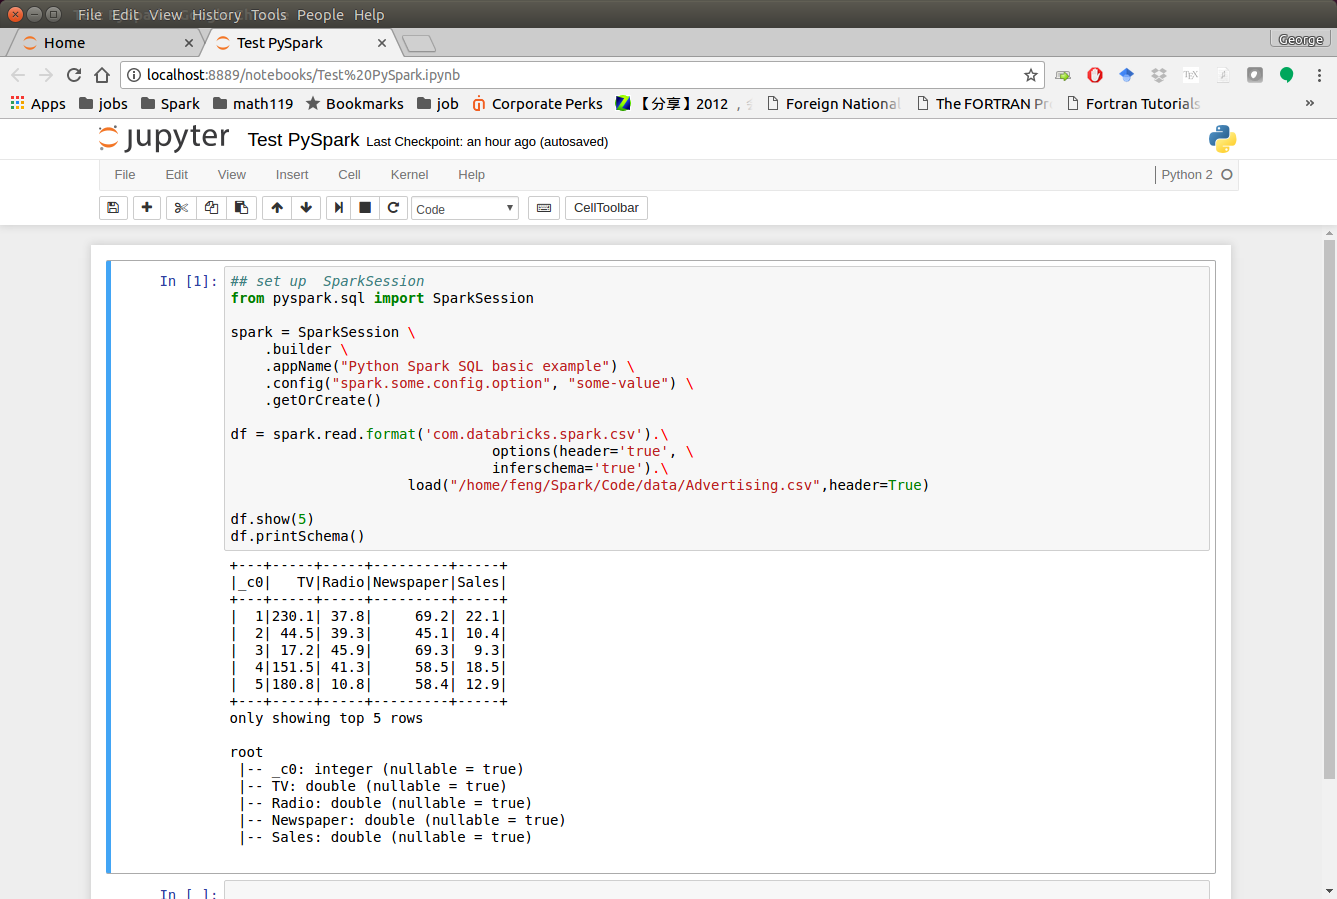
\includegraphics{jupyterWithPySpark.png}
\label{setup:fig-jupyterwithpyspark}\end{figure}
\end{quote}


\subsection{PySpark With Sublime Text}
\label{setup:pyspark-with-sublime-text}
After you finishing the above setup steps in {\hyperref[setup:set-up-ubuntu]{\emph{Configure Spark on Mac and Ubuntu}}},
then you should be good to use Sublime Text to write your PySpark
Code and run your code as a normal python code in Terminal.
\begin{quote}

\begin{Verbatim}[commandchars=\\\{\}]
python test\PYGZus{}pyspark.py
\end{Verbatim}
\end{quote}

Then you should get the output results in your terminal.
\begin{quote}
\begin{figure}[htbp]
\centering

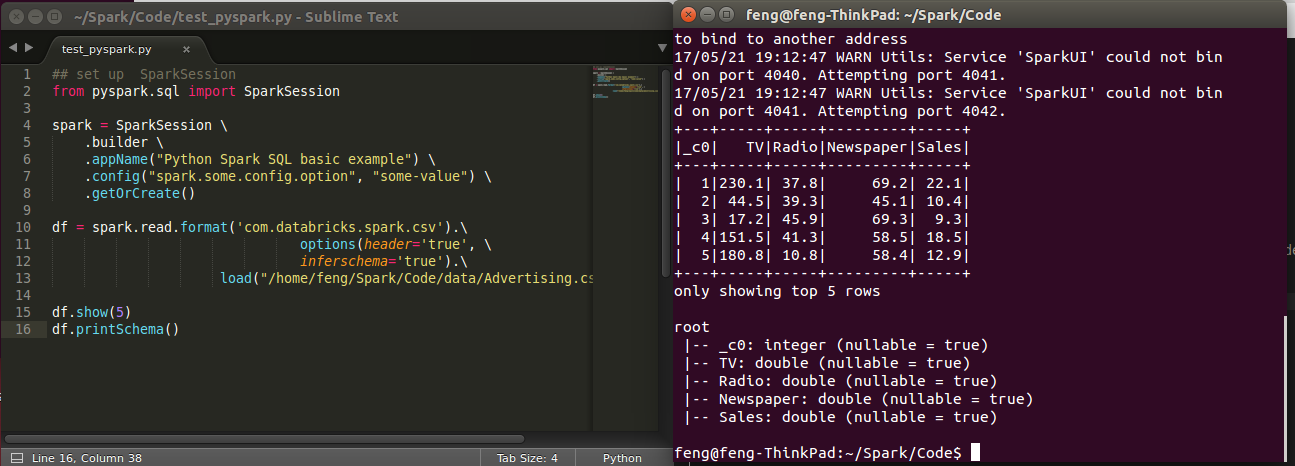
\includegraphics{sublimeWithPySpark.png}
\label{setup:fig-sublimewithpyspark}\end{figure}
\end{quote}


\subsection{PySpark With Eclipse}
\label{setup:pyspark-with-eclipse}
If you want to run PySpark code on Eclipse, you need to add the
paths for the \textbf{External Libraries} for your \textbf{Current Project}
as follows:
\begin{quote}
\begin{enumerate}
\item {} 
Open the properties of your project

\end{enumerate}
\begin{quote}
\begin{figure}[htbp]
\centering

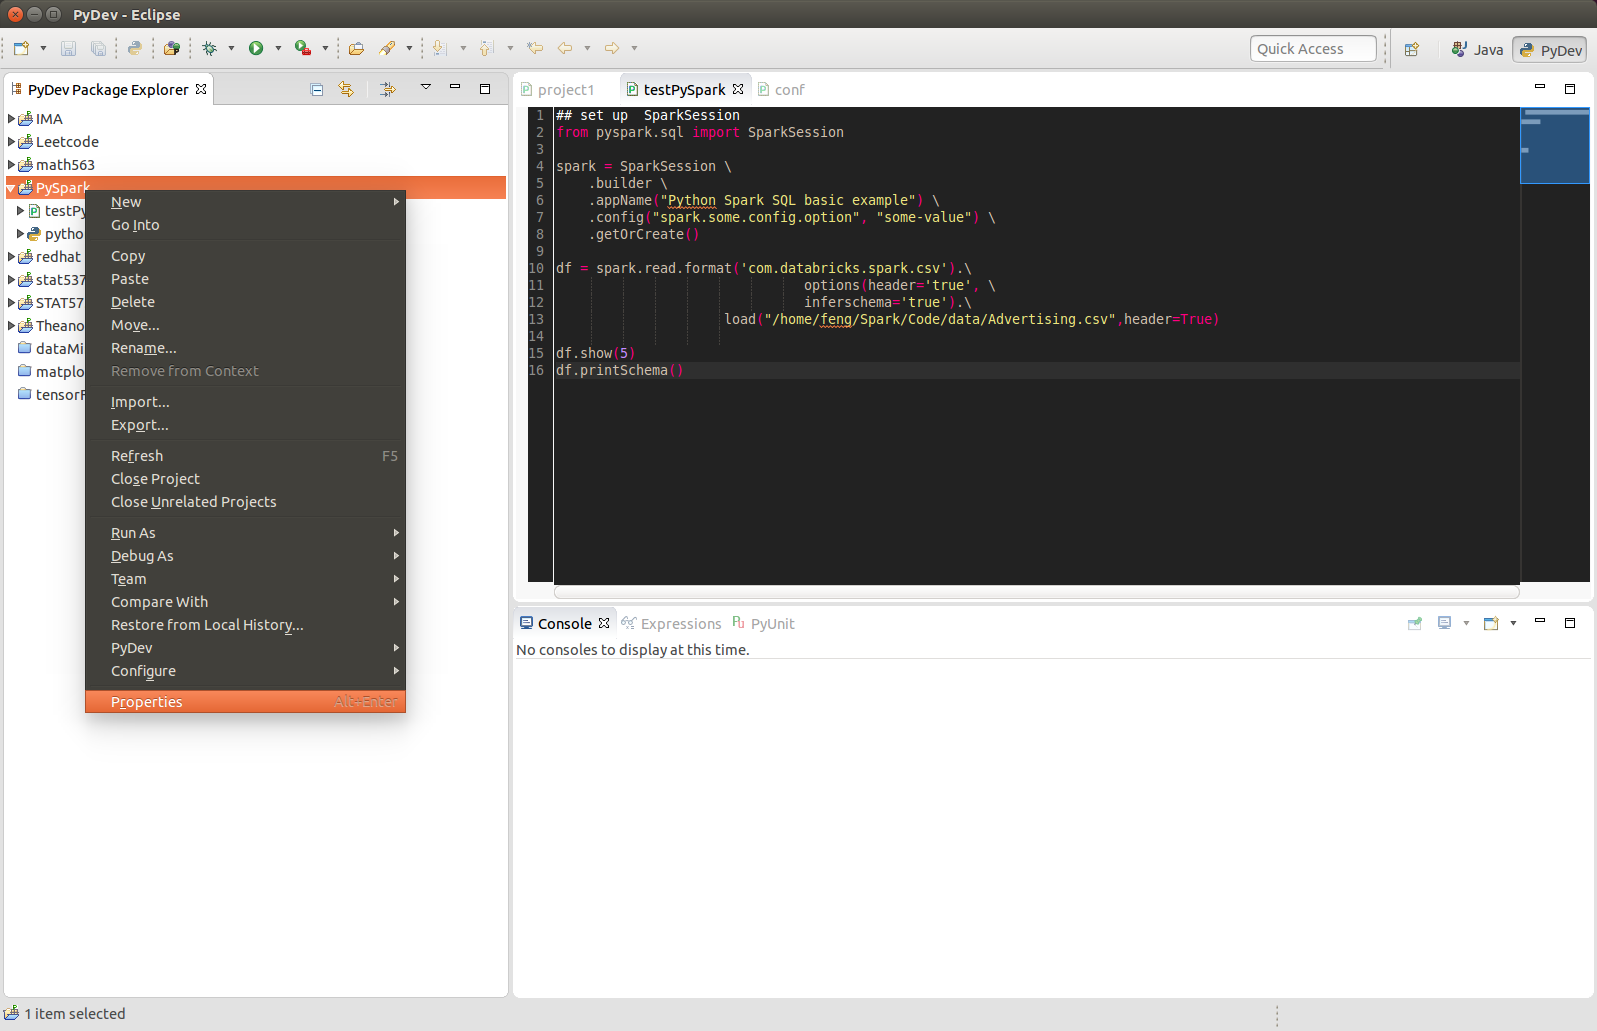
\includegraphics{PyDevProperties.png}
\label{setup:fig-pydevproperties}\end{figure}
\end{quote}
\begin{enumerate}
\setcounter{enumi}{1}
\item {} 
Add the paths for the \textbf{External Libraries}

\end{enumerate}
\begin{quote}
\begin{figure}[htbp]
\centering

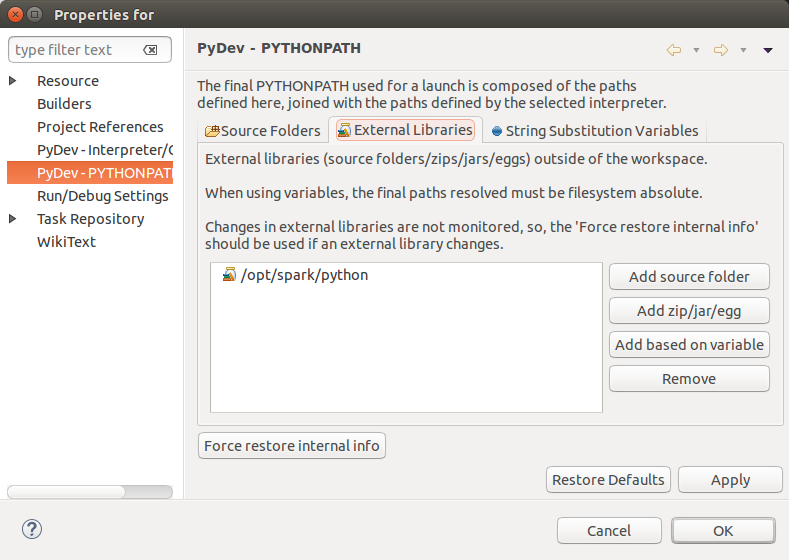
\includegraphics{pydevPath.png}
\label{setup:fig-pydevpath}\end{figure}
\end{quote}
\end{quote}

And then you should be good to run your code on Eclipse with PyDev.
\begin{quote}
\begin{figure}[htbp]
\centering

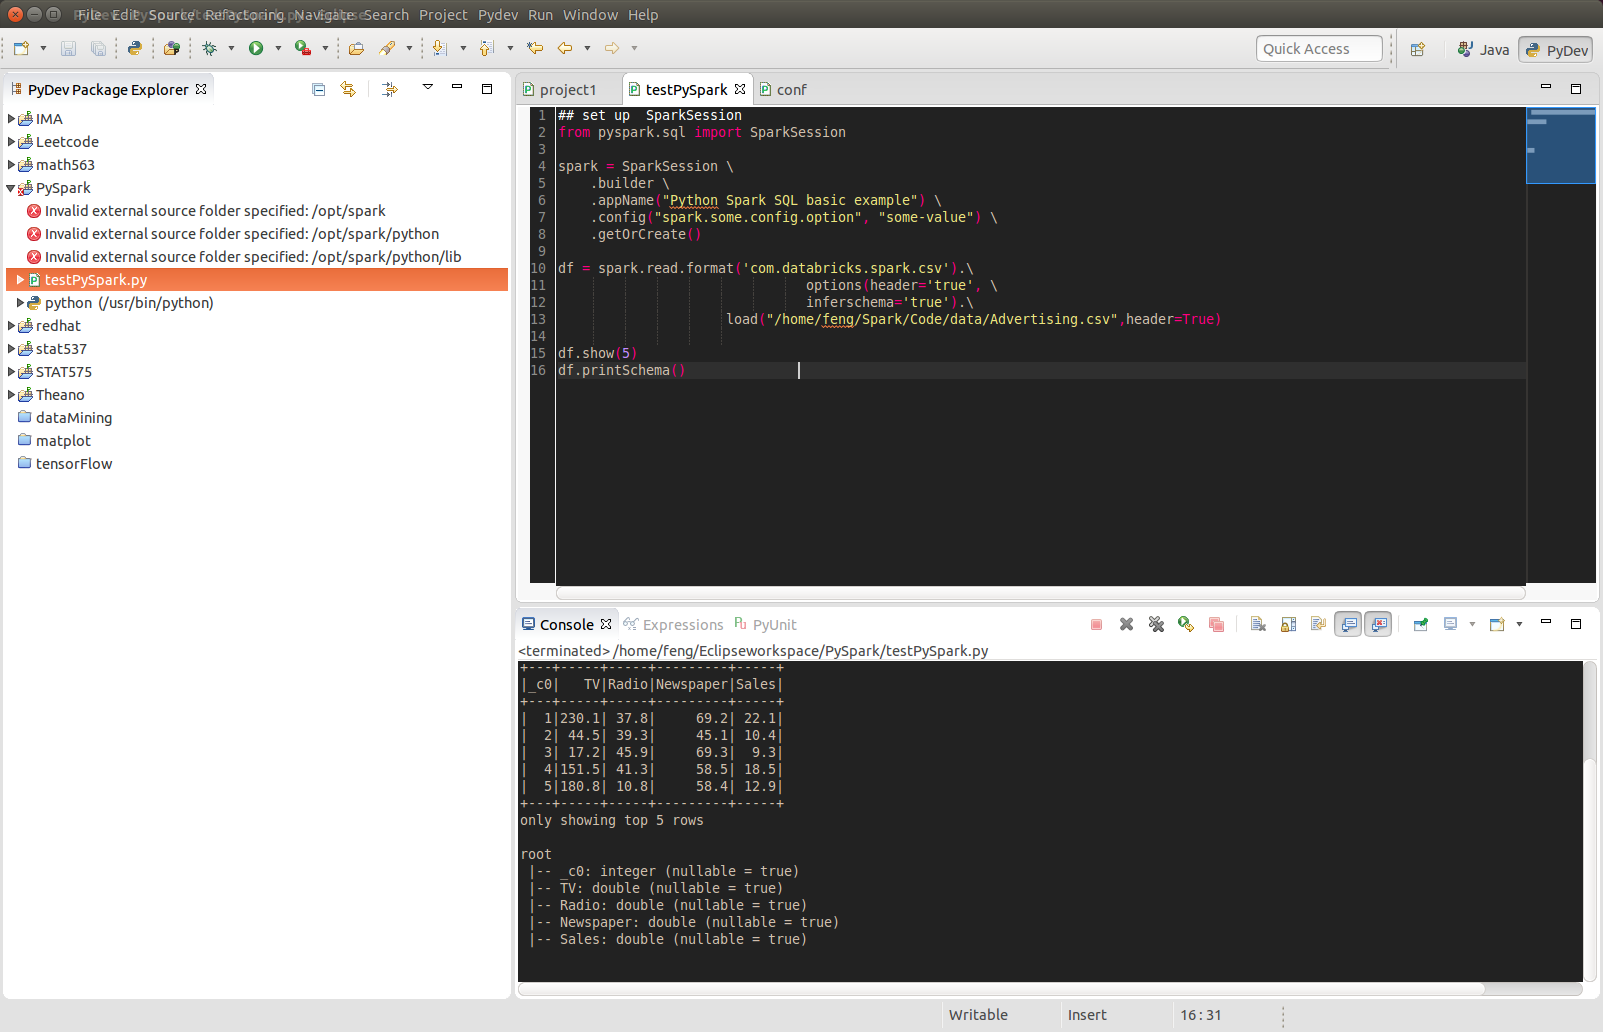
\includegraphics{pysparkWithEclipse.png}
\label{setup:fig-pysparkwitheclipse}\end{figure}
\end{quote}

\index{Set up Spark on Cloud}

\section{Set up Spark on Cloud}
\label{setup:set-up-spark-on-cloud}\label{setup:index-2}
Folloing the setup steps in {\hyperref[setup:set-up-ubuntu]{\emph{Configure Spark on Mac and Ubuntu}}}, you can set
up your own cluster on the cloud, for example AWS, Google Cloud.
Actually, for those clouds, they have their own Big Data tool.
Yon can run them directly whitout any setting just like
Databricks Community Cloud. If you want more details, please feel
free to contact with me.


\section{Demo Code in this Section}
\label{setup:demo-code-in-this-section}
The code for this section is available for download test\_pyspark,
and the Jupyter notebook can be download from test\_pyspark\_ipynb.
\begin{itemize}
\item {} 
Python Source code

\end{itemize}
\begin{quote}

\begin{Verbatim}[commandchars=\\\{\}]
\PYG{c}{\PYGZsh{}\PYGZsh{} set up  SparkSession}
\PYG{k+kn}{from} \PYG{n+nn}{pyspark.sql} \PYG{k+kn}{import} \PYG{n}{SparkSession}

\PYG{n}{spark} \PYG{o}{=} \PYG{n}{SparkSession} \PYGZbs{}
    \PYG{o}{.}\PYG{n}{builder} \PYGZbs{}
    \PYG{o}{.}\PYG{n}{appName}\PYG{p}{(}\PYG{l+s}{\PYGZdq{}}\PYG{l+s}{Python Spark SQL basic example}\PYG{l+s}{\PYGZdq{}}\PYG{p}{)} \PYGZbs{}
    \PYG{o}{.}\PYG{n}{config}\PYG{p}{(}\PYG{l+s}{\PYGZdq{}}\PYG{l+s}{spark.some.config.option}\PYG{l+s}{\PYGZdq{}}\PYG{p}{,} \PYG{l+s}{\PYGZdq{}}\PYG{l+s}{some\PYGZhy{}value}\PYG{l+s}{\PYGZdq{}}\PYG{p}{)} \PYGZbs{}
    \PYG{o}{.}\PYG{n}{getOrCreate}\PYG{p}{(}\PYG{p}{)}

\PYG{n}{df} \PYG{o}{=} \PYG{n}{spark}\PYG{o}{.}\PYG{n}{read}\PYG{o}{.}\PYG{n}{format}\PYG{p}{(}\PYG{l+s}{\PYGZsq{}}\PYG{l+s}{com.databricks.spark.csv}\PYG{l+s}{\PYGZsq{}}\PYG{p}{)}\PYG{o}{.}\PYGZbs{}
                               \PYG{n}{options}\PYG{p}{(}\PYG{n}{header}\PYG{o}{=}\PYG{l+s}{\PYGZsq{}}\PYG{l+s}{true}\PYG{l+s}{\PYGZsq{}}\PYG{p}{,} \PYGZbs{}
                               \PYG{n}{inferschema}\PYG{o}{=}\PYG{l+s}{\PYGZsq{}}\PYG{l+s}{true}\PYG{l+s}{\PYGZsq{}}\PYG{p}{)}\PYG{o}{.}\PYGZbs{}
                     \PYG{n}{load}\PYG{p}{(}\PYG{l+s}{\PYGZdq{}}\PYG{l+s}{/home/feng/Spark/Code/data/Advertising.csv}\PYG{l+s}{\PYGZdq{}}\PYG{p}{,}\PYG{n}{header}\PYG{o}{=}\PYG{n+nb+bp}{True}\PYG{p}{)}

\PYG{n}{df}\PYG{o}{.}\PYG{n}{show}\PYG{p}{(}\PYG{l+m+mi}{5}\PYG{p}{)}
\PYG{n}{df}\PYG{o}{.}\PYG{n}{printSchema}\PYG{p}{(}\PYG{p}{)}
\end{Verbatim}
\end{quote}


\chapter{An Introduction to Apache Spark}
\label{introduction:introduction}\label{introduction:an-introduction-to-apache-spark}\label{introduction:getting-started-with-pyspark-on-windows}\label{introduction::doc}
\begin{notice}{note}{Note:}
\textbf{Know yourself and know your enemy, and you will never be defeated} – idiom, from Sunzi’s Art of War
\end{notice}


\section{Core Concepts}
\label{introduction:core-concepts}
Most of the following content comes from {\hyperref[reference:kirillov2016]{{[}Kirillov2016{]}}}. So the copyright belongs to \textbf{Anton Kirillov}.
I will refer you to get more details from \href{http://datastrophic.io/core-concepts-architecture-and-internals-of-apache-spark/}{Apache Spark core concepts, architecture and internals}.

Before diving deep into how Apache Spark works, lets understand the jargon of Apache Spark
\begin{itemize}
\item {} 
Job: A piece of code which reads some input from HDFS or local, performs some computation on the data and writes some output data.

\item {} 
Stages: Jobs are divided into stages. Stages are classified as a Map or reduce stages (Its easier to understand if you have worked on Hadoop and want to correlate). Stages are divided based on computational boundaries, all computations (operators) cannot be Updated in a single Stage. It happens over many stages.

\item {} 
Tasks: Each stage has some tasks, one task per partition. One task is executed on one partition of data on one executor (machine).

\item {} 
DAG: DAG stands for Directed Acyclic Graph, in the present context its a DAG of operators.

\item {} 
Executor: The process responsible for executing a task.

\item {} 
Master: The machine on which the Driver program runs

\item {} 
Slave: The machine on which the Executor program runs

\end{itemize}


\section{Spark Components}
\label{introduction:spark-components}\begin{quote}
\begin{quote}
\begin{figure}[htbp]
\centering

\includegraphics{spark-components.png}
\label{introduction:fig-spark-components}\end{figure}
\end{quote}
\begin{enumerate}
\item {} 
Spark Driver

\end{enumerate}
\begin{itemize}
\item {} 
separate process to execute user applications

\item {} 
creates SparkContext to schedule jobs execution
and negotiate with cluster manager

\end{itemize}
\begin{enumerate}
\setcounter{enumi}{1}
\item {} 
Executors

\end{enumerate}
\begin{itemize}
\item {} 
run tasks scheduled by driver

\item {} 
store computation results in memory, on disk or off-heap

\item {} 
interact with storage systems

\end{itemize}
\begin{enumerate}
\setcounter{enumi}{2}
\item {} 
Cluster Manager

\end{enumerate}
\begin{itemize}
\item {} 
Mesos

\item {} 
YARN

\item {} 
Spark Standalone

\end{itemize}
\end{quote}

Spark Driver contains more components responsible for translation
of user code into actual jobs executed on cluster:
\begin{quote}
\begin{quote}
\begin{figure}[htbp]
\centering

\includegraphics{spark-components1.png}
\label{introduction:fig-spark-components1}\end{figure}
\end{quote}
\begin{itemize}
\item {} 
SparkContext
\begin{itemize}
\item {} 
represents the connection to a Spark cluster, and can be used to create RDDs,
accumulators and broadcast variables  on that cluster

\end{itemize}

\item {} 
DAGScheduler
\begin{itemize}
\item {} 
computes a DAG of stages for each job and submits them to TaskScheduler
determines preferred locations for tasks (based on cache status or
shuffle files locations) and finds minimum schedule to run the jobs

\end{itemize}

\item {} 
TaskScheduler
\begin{itemize}
\item {} 
responsible for sending tasks to the cluster, running them,
retrying if there are failures, and mitigating stragglers

\end{itemize}

\item {} 
SchedulerBackend
\begin{itemize}
\item {} 
backend interface for scheduling systems that allows plugging
in different implementations(Mesos, YARN, Standalone, local)

\end{itemize}

\item {} 
BlockManager
\begin{itemize}
\item {} 
provides interfaces for putting and retrieving blocks both locally
and remotely into various stores (memory,  disk, and off-heap)

\end{itemize}

\end{itemize}
\end{quote}


\section{Architecture}
\label{introduction:architecture}

\section{How Spark Works?}
\label{introduction:how-spark-works}
Spark has a small code base and the system is divided in various layers. Each layer has some responsibilities. The layers are independent of each other.

The first layer is the interpreter, Spark uses a Scala interpreter, with some modifications.
As you enter your code in spark console (creating RDD’s and applying operators), Spark creates a operator graph.
When the user runs an action (like collect), the Graph is submitted to a DAG Scheduler. The DAG scheduler divides operator graph into (map and reduce) stages.
A stage is comprised of tasks based on partitions of the input data. The DAG scheduler pipelines operators together to optimize the graph. For e.g. Many map operators can be scheduled in a single stage. This optimization is key to Sparks performance. The final result of a DAG scheduler is a set of stages.
The stages are passed on to the Task Scheduler. The task scheduler launches tasks via cluster manager. (Spark Standalone/Yarn/Mesos). The task scheduler doesn’t know about dependencies among stages.
\begin{quote}
\begin{figure}[htbp]
\centering

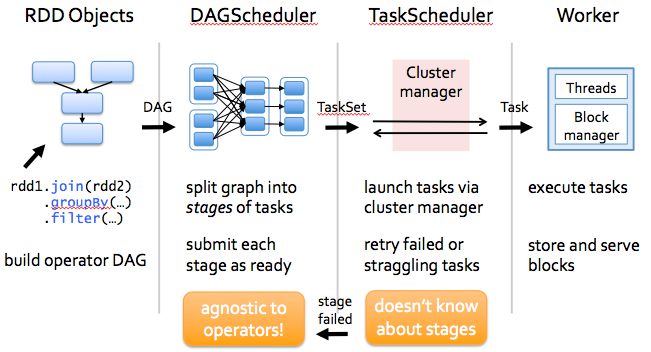
\includegraphics{work_flow.png}
\label{introduction:fig-workflow}\end{figure}
\end{quote}


\chapter{Programming with RDDs}
\label{rdd:apache-spark-core-concepts-architecture-and-internals}\label{rdd:rdd}\label{rdd::doc}\label{rdd:programming-with-rdds}
\begin{notice}{note}{Note:}
\textbf{If you only know yourself, but not your opponent, you may win or may lose.
If you know neither yourself nor your enemy, you will always endanger yourself}
– idiom, from Sunzi’s Art of War
\end{notice}

RDD represents \textbf{Resilient Distributed Dataset}. An RDD in Spark is simply an immutable
distributed collection of objects sets. Each RDD is split into multiple partitions (similar pattern
with smaller sets), which may be computed on different nodes of the cluster.


\section{Create RDD}
\label{rdd:create-rdd}
Usually, there are two popular way to create the RDDs: loading an external dataset, or distributing
a set of collection of objects. The following examples show some simplest ways to create RDDs by using
\code{parallelize()} fucntion which takes an already existing collection in your program and pass the same
to the Spark Context.
\begin{enumerate}
\item {} 
By using \code{parallelize( )} fucntion

\end{enumerate}

\begin{Verbatim}[commandchars=\\\{\}]
\PYG{k+kn}{from} \PYG{n+nn}{pyspark.sql} \PYG{k+kn}{import} \PYG{n}{SparkSession}

\PYG{n}{spark} \PYG{o}{=} \PYG{n}{SparkSession} \PYGZbs{}
    \PYG{o}{.}\PYG{n}{builder} \PYGZbs{}
    \PYG{o}{.}\PYG{n}{appName}\PYG{p}{(}\PYG{l+s}{\PYGZdq{}}\PYG{l+s}{Python Spark create RDD example}\PYG{l+s}{\PYGZdq{}}\PYG{p}{)} \PYGZbs{}
    \PYG{o}{.}\PYG{n}{config}\PYG{p}{(}\PYG{l+s}{\PYGZdq{}}\PYG{l+s}{spark.some.config.option}\PYG{l+s}{\PYGZdq{}}\PYG{p}{,} \PYG{l+s}{\PYGZdq{}}\PYG{l+s}{some\PYGZhy{}value}\PYG{l+s}{\PYGZdq{}}\PYG{p}{)} \PYGZbs{}
    \PYG{o}{.}\PYG{n}{getOrCreate}\PYG{p}{(}\PYG{p}{)}

\PYG{n}{df} \PYG{o}{=} \PYG{n}{spark}\PYG{o}{.}\PYG{n}{sparkContext}\PYG{o}{.}\PYG{n}{parallelize}\PYG{p}{(}\PYG{p}{[}\PYG{p}{(}\PYG{l+m+mi}{1}\PYG{p}{,} \PYG{l+m+mi}{2}\PYG{p}{,} \PYG{l+m+mi}{3}\PYG{p}{,} \PYG{l+s}{\PYGZsq{}}\PYG{l+s}{a b c}\PYG{l+s}{\PYGZsq{}}\PYG{p}{)}\PYG{p}{,}
             \PYG{p}{(}\PYG{l+m+mi}{4}\PYG{p}{,} \PYG{l+m+mi}{5}\PYG{p}{,} \PYG{l+m+mi}{6}\PYG{p}{,} \PYG{l+s}{\PYGZsq{}}\PYG{l+s}{d e f}\PYG{l+s}{\PYGZsq{}}\PYG{p}{)}\PYG{p}{,}
             \PYG{p}{(}\PYG{l+m+mi}{7}\PYG{p}{,} \PYG{l+m+mi}{8}\PYG{p}{,} \PYG{l+m+mi}{9}\PYG{p}{,} \PYG{l+s}{\PYGZsq{}}\PYG{l+s}{g h i}\PYG{l+s}{\PYGZsq{}}\PYG{p}{)}\PYG{p}{]}\PYG{p}{)}\PYG{o}{.}\PYG{n}{toDF}\PYG{p}{(}\PYG{p}{[}\PYG{l+s}{\PYGZsq{}}\PYG{l+s}{col1}\PYG{l+s}{\PYGZsq{}}\PYG{p}{,} \PYG{l+s}{\PYGZsq{}}\PYG{l+s}{col2}\PYG{l+s}{\PYGZsq{}}\PYG{p}{,} \PYG{l+s}{\PYGZsq{}}\PYG{l+s}{col3}\PYG{l+s}{\PYGZsq{}}\PYG{p}{,}\PYG{l+s}{\PYGZsq{}}\PYG{l+s}{col4}\PYG{l+s}{\PYGZsq{}}\PYG{p}{]}\PYG{p}{)}
\end{Verbatim}

Then you will get the RDD data:

\begin{Verbatim}[commandchars=\\\{\}]
\PYG{n}{df}\PYG{o}{.}\PYG{n}{show}\PYG{p}{(}\PYG{p}{)}

\PYG{o}{+}\PYG{o}{\PYGZhy{}}\PYG{o}{\PYGZhy{}}\PYG{o}{\PYGZhy{}}\PYG{o}{\PYGZhy{}}\PYG{o}{+}\PYG{o}{\PYGZhy{}}\PYG{o}{\PYGZhy{}}\PYG{o}{\PYGZhy{}}\PYG{o}{\PYGZhy{}}\PYG{o}{+}\PYG{o}{\PYGZhy{}}\PYG{o}{\PYGZhy{}}\PYG{o}{\PYGZhy{}}\PYG{o}{\PYGZhy{}}\PYG{o}{+}\PYG{o}{\PYGZhy{}}\PYG{o}{\PYGZhy{}}\PYG{o}{\PYGZhy{}}\PYG{o}{\PYGZhy{}}\PYG{o}{\PYGZhy{}}\PYG{o}{+}
\PYG{o}{\textbar{}}\PYG{n}{col1}\PYG{o}{\textbar{}}\PYG{n}{col2}\PYG{o}{\textbar{}}\PYG{n}{col3}\PYG{o}{\textbar{}} \PYG{n}{col4}\PYG{o}{\textbar{}}
\PYG{o}{+}\PYG{o}{\PYGZhy{}}\PYG{o}{\PYGZhy{}}\PYG{o}{\PYGZhy{}}\PYG{o}{\PYGZhy{}}\PYG{o}{+}\PYG{o}{\PYGZhy{}}\PYG{o}{\PYGZhy{}}\PYG{o}{\PYGZhy{}}\PYG{o}{\PYGZhy{}}\PYG{o}{+}\PYG{o}{\PYGZhy{}}\PYG{o}{\PYGZhy{}}\PYG{o}{\PYGZhy{}}\PYG{o}{\PYGZhy{}}\PYG{o}{+}\PYG{o}{\PYGZhy{}}\PYG{o}{\PYGZhy{}}\PYG{o}{\PYGZhy{}}\PYG{o}{\PYGZhy{}}\PYG{o}{\PYGZhy{}}\PYG{o}{+}
\PYG{o}{\textbar{}}   \PYG{l+m+mi}{1}\PYG{o}{\textbar{}}   \PYG{l+m+mi}{2}\PYG{o}{\textbar{}}   \PYG{l+m+mi}{3}\PYG{o}{\textbar{}}\PYG{n}{a} \PYG{n}{b} \PYG{n}{c}\PYG{o}{\textbar{}}
\PYG{o}{\textbar{}}   \PYG{l+m+mi}{4}\PYG{o}{\textbar{}}   \PYG{l+m+mi}{5}\PYG{o}{\textbar{}}   \PYG{l+m+mi}{6}\PYG{o}{\textbar{}}\PYG{n}{d} \PYG{n}{e} \PYG{n}{f}\PYG{o}{\textbar{}}
\PYG{o}{\textbar{}}   \PYG{l+m+mi}{7}\PYG{o}{\textbar{}}   \PYG{l+m+mi}{8}\PYG{o}{\textbar{}}   \PYG{l+m+mi}{9}\PYG{o}{\textbar{}}\PYG{n}{g} \PYG{n}{h} \PYG{n}{i}\PYG{o}{\textbar{}}
\PYG{o}{+}\PYG{o}{\PYGZhy{}}\PYG{o}{\PYGZhy{}}\PYG{o}{\PYGZhy{}}\PYG{o}{\PYGZhy{}}\PYG{o}{+}\PYG{o}{\PYGZhy{}}\PYG{o}{\PYGZhy{}}\PYG{o}{\PYGZhy{}}\PYG{o}{\PYGZhy{}}\PYG{o}{+}\PYG{o}{\PYGZhy{}}\PYG{o}{\PYGZhy{}}\PYG{o}{\PYGZhy{}}\PYG{o}{\PYGZhy{}}\PYG{o}{+}\PYG{o}{\PYGZhy{}}\PYG{o}{\PYGZhy{}}\PYG{o}{\PYGZhy{}}\PYG{o}{\PYGZhy{}}\PYG{o}{\PYGZhy{}}\PYG{o}{+}
\end{Verbatim}

\begin{Verbatim}[commandchars=\\\{\}]
\PYG{k+kn}{from} \PYG{n+nn}{pyspark.sql} \PYG{k+kn}{import} \PYG{n}{SparkSession}

\PYG{n}{spark} \PYG{o}{=} \PYG{n}{SparkSession} \PYGZbs{}
    \PYG{o}{.}\PYG{n}{builder} \PYGZbs{}
    \PYG{o}{.}\PYG{n}{appName}\PYG{p}{(}\PYG{l+s}{\PYGZdq{}}\PYG{l+s}{Python Spark create RDD example}\PYG{l+s}{\PYGZdq{}}\PYG{p}{)} \PYGZbs{}
    \PYG{o}{.}\PYG{n}{config}\PYG{p}{(}\PYG{l+s}{\PYGZdq{}}\PYG{l+s}{spark.some.config.option}\PYG{l+s}{\PYGZdq{}}\PYG{p}{,} \PYG{l+s}{\PYGZdq{}}\PYG{l+s}{some\PYGZhy{}value}\PYG{l+s}{\PYGZdq{}}\PYG{p}{)} \PYGZbs{}
    \PYG{o}{.}\PYG{n}{getOrCreate}\PYG{p}{(}\PYG{p}{)}

\PYG{n}{myData} \PYG{o}{=} \PYG{n}{spark}\PYG{o}{.}\PYG{n}{sparkContext}\PYG{o}{.}\PYG{n}{parallelize}\PYG{p}{(}\PYG{p}{[}\PYG{p}{(}\PYG{l+m+mi}{1}\PYG{p}{,}\PYG{l+m+mi}{2}\PYG{p}{)}\PYG{p}{,} \PYG{p}{(}\PYG{l+m+mi}{3}\PYG{p}{,}\PYG{l+m+mi}{4}\PYG{p}{)}\PYG{p}{,} \PYG{p}{(}\PYG{l+m+mi}{5}\PYG{p}{,}\PYG{l+m+mi}{6}\PYG{p}{)}\PYG{p}{,} \PYG{p}{(}\PYG{l+m+mi}{7}\PYG{p}{,}\PYG{l+m+mi}{8}\PYG{p}{)}\PYG{p}{,} \PYG{p}{(}\PYG{l+m+mi}{9}\PYG{p}{,}\PYG{l+m+mi}{10}\PYG{p}{)}\PYG{p}{]}\PYG{p}{)}
\end{Verbatim}

Then you will get the RDD data:

\begin{Verbatim}[commandchars=\\\{\}]
\PYG{n}{myData}\PYG{o}{.}\PYG{n}{collect}\PYG{p}{(}\PYG{p}{)}

\PYG{p}{[}\PYG{p}{(}\PYG{l+m+mi}{1}\PYG{p}{,} \PYG{l+m+mi}{2}\PYG{p}{)}\PYG{p}{,} \PYG{p}{(}\PYG{l+m+mi}{3}\PYG{p}{,} \PYG{l+m+mi}{4}\PYG{p}{)}\PYG{p}{,} \PYG{p}{(}\PYG{l+m+mi}{5}\PYG{p}{,} \PYG{l+m+mi}{6}\PYG{p}{)}\PYG{p}{,} \PYG{p}{(}\PYG{l+m+mi}{7}\PYG{p}{,} \PYG{l+m+mi}{8}\PYG{p}{)}\PYG{p}{,} \PYG{p}{(}\PYG{l+m+mi}{9}\PYG{p}{,} \PYG{l+m+mi}{10}\PYG{p}{)}\PYG{p}{]}
\end{Verbatim}
\begin{enumerate}
\setcounter{enumi}{1}
\item {} 
By using \code{createDataFrame( )} function

\end{enumerate}

\begin{Verbatim}[commandchars=\\\{\}]
\PYG{k+kn}{from} \PYG{n+nn}{pyspark.sql} \PYG{k+kn}{import} \PYG{n}{SparkSession}

\PYG{n}{spark} \PYG{o}{=} \PYG{n}{SparkSession} \PYGZbs{}
    \PYG{o}{.}\PYG{n}{builder} \PYGZbs{}
    \PYG{o}{.}\PYG{n}{appName}\PYG{p}{(}\PYG{l+s}{\PYGZdq{}}\PYG{l+s}{Python Spark create RDD example}\PYG{l+s}{\PYGZdq{}}\PYG{p}{)} \PYGZbs{}
    \PYG{o}{.}\PYG{n}{config}\PYG{p}{(}\PYG{l+s}{\PYGZdq{}}\PYG{l+s}{spark.some.config.option}\PYG{l+s}{\PYGZdq{}}\PYG{p}{,} \PYG{l+s}{\PYGZdq{}}\PYG{l+s}{some\PYGZhy{}value}\PYG{l+s}{\PYGZdq{}}\PYG{p}{)} \PYGZbs{}
    \PYG{o}{.}\PYG{n}{getOrCreate}\PYG{p}{(}\PYG{p}{)}

\PYG{n}{Employee} \PYG{o}{=} \PYG{n}{spark}\PYG{o}{.}\PYG{n}{createDataFrame}\PYG{p}{(}\PYG{p}{[}
                        \PYG{p}{(}\PYG{l+s}{\PYGZsq{}}\PYG{l+s}{1}\PYG{l+s}{\PYGZsq{}}\PYG{p}{,} \PYG{l+s}{\PYGZsq{}}\PYG{l+s}{Joe}\PYG{l+s}{\PYGZsq{}}\PYG{p}{,}   \PYG{l+s}{\PYGZsq{}}\PYG{l+s}{70000}\PYG{l+s}{\PYGZsq{}}\PYG{p}{,} \PYG{l+s}{\PYGZsq{}}\PYG{l+s}{1}\PYG{l+s}{\PYGZsq{}}\PYG{p}{)}\PYG{p}{,}
                        \PYG{p}{(}\PYG{l+s}{\PYGZsq{}}\PYG{l+s}{2}\PYG{l+s}{\PYGZsq{}}\PYG{p}{,} \PYG{l+s}{\PYGZsq{}}\PYG{l+s}{Henry}\PYG{l+s}{\PYGZsq{}}\PYG{p}{,} \PYG{l+s}{\PYGZsq{}}\PYG{l+s}{80000}\PYG{l+s}{\PYGZsq{}}\PYG{p}{,} \PYG{l+s}{\PYGZsq{}}\PYG{l+s}{2}\PYG{l+s}{\PYGZsq{}}\PYG{p}{)}\PYG{p}{,}
                        \PYG{p}{(}\PYG{l+s}{\PYGZsq{}}\PYG{l+s}{3}\PYG{l+s}{\PYGZsq{}}\PYG{p}{,} \PYG{l+s}{\PYGZsq{}}\PYG{l+s}{Sam}\PYG{l+s}{\PYGZsq{}}\PYG{p}{,}   \PYG{l+s}{\PYGZsq{}}\PYG{l+s}{60000}\PYG{l+s}{\PYGZsq{}}\PYG{p}{,} \PYG{l+s}{\PYGZsq{}}\PYG{l+s}{2}\PYG{l+s}{\PYGZsq{}}\PYG{p}{)}\PYG{p}{,}
                        \PYG{p}{(}\PYG{l+s}{\PYGZsq{}}\PYG{l+s}{4}\PYG{l+s}{\PYGZsq{}}\PYG{p}{,} \PYG{l+s}{\PYGZsq{}}\PYG{l+s}{Max}\PYG{l+s}{\PYGZsq{}}\PYG{p}{,}   \PYG{l+s}{\PYGZsq{}}\PYG{l+s}{90000}\PYG{l+s}{\PYGZsq{}}\PYG{p}{,} \PYG{l+s}{\PYGZsq{}}\PYG{l+s}{1}\PYG{l+s}{\PYGZsq{}}\PYG{p}{)}\PYG{p}{]}\PYG{p}{,}
                        \PYG{p}{[}\PYG{l+s}{\PYGZsq{}}\PYG{l+s}{Id}\PYG{l+s}{\PYGZsq{}}\PYG{p}{,} \PYG{l+s}{\PYGZsq{}}\PYG{l+s}{Name}\PYG{l+s}{\PYGZsq{}}\PYG{p}{,} \PYG{l+s}{\PYGZsq{}}\PYG{l+s}{Sallary}\PYG{l+s}{\PYGZsq{}}\PYG{p}{,}\PYG{l+s}{\PYGZsq{}}\PYG{l+s}{DepartmentId}\PYG{l+s}{\PYGZsq{}}\PYG{p}{]}
                       \PYG{p}{)}
\end{Verbatim}

Then you will get the RDD data:

\begin{Verbatim}[commandchars=\\\{\}]
\PYG{o}{+}\PYG{o}{\PYGZhy{}}\PYG{o}{\PYGZhy{}}\PYG{o}{\PYGZhy{}}\PYG{o}{+}\PYG{o}{\PYGZhy{}}\PYG{o}{\PYGZhy{}}\PYG{o}{\PYGZhy{}}\PYG{o}{\PYGZhy{}}\PYG{o}{\PYGZhy{}}\PYG{o}{+}\PYG{o}{\PYGZhy{}}\PYG{o}{\PYGZhy{}}\PYG{o}{\PYGZhy{}}\PYG{o}{\PYGZhy{}}\PYG{o}{\PYGZhy{}}\PYG{o}{\PYGZhy{}}\PYG{o}{\PYGZhy{}}\PYG{o}{+}\PYG{o}{\PYGZhy{}}\PYG{o}{\PYGZhy{}}\PYG{o}{\PYGZhy{}}\PYG{o}{\PYGZhy{}}\PYG{o}{\PYGZhy{}}\PYG{o}{\PYGZhy{}}\PYG{o}{\PYGZhy{}}\PYG{o}{\PYGZhy{}}\PYG{o}{\PYGZhy{}}\PYG{o}{\PYGZhy{}}\PYG{o}{\PYGZhy{}}\PYG{o}{\PYGZhy{}}\PYG{o}{+}
\PYG{o}{\textbar{}} \PYG{n}{Id}\PYG{o}{\textbar{}} \PYG{n}{Name}\PYG{o}{\textbar{}}\PYG{n}{Sallary}\PYG{o}{\textbar{}}\PYG{n}{DepartmentId}\PYG{o}{\textbar{}}
\PYG{o}{+}\PYG{o}{\PYGZhy{}}\PYG{o}{\PYGZhy{}}\PYG{o}{\PYGZhy{}}\PYG{o}{+}\PYG{o}{\PYGZhy{}}\PYG{o}{\PYGZhy{}}\PYG{o}{\PYGZhy{}}\PYG{o}{\PYGZhy{}}\PYG{o}{\PYGZhy{}}\PYG{o}{+}\PYG{o}{\PYGZhy{}}\PYG{o}{\PYGZhy{}}\PYG{o}{\PYGZhy{}}\PYG{o}{\PYGZhy{}}\PYG{o}{\PYGZhy{}}\PYG{o}{\PYGZhy{}}\PYG{o}{\PYGZhy{}}\PYG{o}{+}\PYG{o}{\PYGZhy{}}\PYG{o}{\PYGZhy{}}\PYG{o}{\PYGZhy{}}\PYG{o}{\PYGZhy{}}\PYG{o}{\PYGZhy{}}\PYG{o}{\PYGZhy{}}\PYG{o}{\PYGZhy{}}\PYG{o}{\PYGZhy{}}\PYG{o}{\PYGZhy{}}\PYG{o}{\PYGZhy{}}\PYG{o}{\PYGZhy{}}\PYG{o}{\PYGZhy{}}\PYG{o}{+}
\PYG{o}{\textbar{}}  \PYG{l+m+mi}{1}\PYG{o}{\textbar{}}  \PYG{n}{Joe}\PYG{o}{\textbar{}}  \PYG{l+m+mi}{70000}\PYG{o}{\textbar{}}           \PYG{l+m+mi}{1}\PYG{o}{\textbar{}}
\PYG{o}{\textbar{}}  \PYG{l+m+mi}{2}\PYG{o}{\textbar{}}\PYG{n}{Henry}\PYG{o}{\textbar{}}  \PYG{l+m+mi}{80000}\PYG{o}{\textbar{}}           \PYG{l+m+mi}{2}\PYG{o}{\textbar{}}
\PYG{o}{\textbar{}}  \PYG{l+m+mi}{3}\PYG{o}{\textbar{}}  \PYG{n}{Sam}\PYG{o}{\textbar{}}  \PYG{l+m+mi}{60000}\PYG{o}{\textbar{}}           \PYG{l+m+mi}{2}\PYG{o}{\textbar{}}
\PYG{o}{\textbar{}}  \PYG{l+m+mi}{4}\PYG{o}{\textbar{}}  \PYG{n}{Max}\PYG{o}{\textbar{}}  \PYG{l+m+mi}{90000}\PYG{o}{\textbar{}}           \PYG{l+m+mi}{1}\PYG{o}{\textbar{}}
\PYG{o}{+}\PYG{o}{\PYGZhy{}}\PYG{o}{\PYGZhy{}}\PYG{o}{\PYGZhy{}}\PYG{o}{+}\PYG{o}{\PYGZhy{}}\PYG{o}{\PYGZhy{}}\PYG{o}{\PYGZhy{}}\PYG{o}{\PYGZhy{}}\PYG{o}{\PYGZhy{}}\PYG{o}{+}\PYG{o}{\PYGZhy{}}\PYG{o}{\PYGZhy{}}\PYG{o}{\PYGZhy{}}\PYG{o}{\PYGZhy{}}\PYG{o}{\PYGZhy{}}\PYG{o}{\PYGZhy{}}\PYG{o}{\PYGZhy{}}\PYG{o}{+}\PYG{o}{\PYGZhy{}}\PYG{o}{\PYGZhy{}}\PYG{o}{\PYGZhy{}}\PYG{o}{\PYGZhy{}}\PYG{o}{\PYGZhy{}}\PYG{o}{\PYGZhy{}}\PYG{o}{\PYGZhy{}}\PYG{o}{\PYGZhy{}}\PYG{o}{\PYGZhy{}}\PYG{o}{\PYGZhy{}}\PYG{o}{\PYGZhy{}}\PYG{o}{\PYGZhy{}}\PYG{o}{+}
\end{Verbatim}
\begin{enumerate}
\setcounter{enumi}{2}
\item {} 
By using \code{read} and \code{load} functions

\end{enumerate}
\begin{quote}
\begin{enumerate}
\item {} 
\textbf{Read dataset from .csv file}

\end{enumerate}

\begin{Verbatim}[commandchars=\\\{\}]
\PYG{c}{\PYGZsh{}\PYGZsh{} set up  SparkSession}
\PYG{k+kn}{from} \PYG{n+nn}{pyspark.sql} \PYG{k+kn}{import} \PYG{n}{SparkSession}

\PYG{n}{spark} \PYG{o}{=} \PYG{n}{SparkSession} \PYGZbs{}
    \PYG{o}{.}\PYG{n}{builder} \PYGZbs{}
    \PYG{o}{.}\PYG{n}{appName}\PYG{p}{(}\PYG{l+s}{\PYGZdq{}}\PYG{l+s}{Python Spark create RDD example}\PYG{l+s}{\PYGZdq{}}\PYG{p}{)} \PYGZbs{}
    \PYG{o}{.}\PYG{n}{config}\PYG{p}{(}\PYG{l+s}{\PYGZdq{}}\PYG{l+s}{spark.some.config.option}\PYG{l+s}{\PYGZdq{}}\PYG{p}{,} \PYG{l+s}{\PYGZdq{}}\PYG{l+s}{some\PYGZhy{}value}\PYG{l+s}{\PYGZdq{}}\PYG{p}{)} \PYGZbs{}
    \PYG{o}{.}\PYG{n}{getOrCreate}\PYG{p}{(}\PYG{p}{)}

\PYG{n}{df} \PYG{o}{=} \PYG{n}{spark}\PYG{o}{.}\PYG{n}{read}\PYG{o}{.}\PYG{n}{format}\PYG{p}{(}\PYG{l+s}{\PYGZsq{}}\PYG{l+s}{com.databricks.spark.csv}\PYG{l+s}{\PYGZsq{}}\PYG{p}{)}\PYG{o}{.}\PYGZbs{}
                               \PYG{n}{options}\PYG{p}{(}\PYG{n}{header}\PYG{o}{=}\PYG{l+s}{\PYGZsq{}}\PYG{l+s}{true}\PYG{l+s}{\PYGZsq{}}\PYG{p}{,} \PYGZbs{}
                               \PYG{n}{inferschema}\PYG{o}{=}\PYG{l+s}{\PYGZsq{}}\PYG{l+s}{true}\PYG{l+s}{\PYGZsq{}}\PYG{p}{)}\PYG{o}{.}\PYGZbs{}
                \PYG{n}{load}\PYG{p}{(}\PYG{l+s}{\PYGZdq{}}\PYG{l+s}{/home/feng/Spark/Code/data/Advertising.csv}\PYG{l+s}{\PYGZdq{}}\PYG{p}{,}\PYG{n}{header}\PYG{o}{=}\PYG{n+nb+bp}{True}\PYG{p}{)}

\PYG{n}{df}\PYG{o}{.}\PYG{n}{show}\PYG{p}{(}\PYG{l+m+mi}{5}\PYG{p}{)}
\PYG{n}{df}\PYG{o}{.}\PYG{n}{printSchema}\PYG{p}{(}\PYG{p}{)}
\end{Verbatim}

Then you will get the RDD data:

\begin{Verbatim}[commandchars=\\\{\}]
\PYG{o}{+}\PYG{o}{\PYGZhy{}}\PYG{o}{\PYGZhy{}}\PYG{o}{\PYGZhy{}}\PYG{o}{+}\PYG{o}{\PYGZhy{}}\PYG{o}{\PYGZhy{}}\PYG{o}{\PYGZhy{}}\PYG{o}{\PYGZhy{}}\PYG{o}{\PYGZhy{}}\PYG{o}{+}\PYG{o}{\PYGZhy{}}\PYG{o}{\PYGZhy{}}\PYG{o}{\PYGZhy{}}\PYG{o}{\PYGZhy{}}\PYG{o}{\PYGZhy{}}\PYG{o}{+}\PYG{o}{\PYGZhy{}}\PYG{o}{\PYGZhy{}}\PYG{o}{\PYGZhy{}}\PYG{o}{\PYGZhy{}}\PYG{o}{\PYGZhy{}}\PYG{o}{\PYGZhy{}}\PYG{o}{\PYGZhy{}}\PYG{o}{\PYGZhy{}}\PYG{o}{\PYGZhy{}}\PYG{o}{+}\PYG{o}{\PYGZhy{}}\PYG{o}{\PYGZhy{}}\PYG{o}{\PYGZhy{}}\PYG{o}{\PYGZhy{}}\PYG{o}{\PYGZhy{}}\PYG{o}{+}
\PYG{o}{\textbar{}}\PYG{n}{\PYGZus{}c0}\PYG{o}{\textbar{}}   \PYG{n}{TV}\PYG{o}{\textbar{}}\PYG{n}{Radio}\PYG{o}{\textbar{}}\PYG{n}{Newspaper}\PYG{o}{\textbar{}}\PYG{n}{Sales}\PYG{o}{\textbar{}}
\PYG{o}{+}\PYG{o}{\PYGZhy{}}\PYG{o}{\PYGZhy{}}\PYG{o}{\PYGZhy{}}\PYG{o}{+}\PYG{o}{\PYGZhy{}}\PYG{o}{\PYGZhy{}}\PYG{o}{\PYGZhy{}}\PYG{o}{\PYGZhy{}}\PYG{o}{\PYGZhy{}}\PYG{o}{+}\PYG{o}{\PYGZhy{}}\PYG{o}{\PYGZhy{}}\PYG{o}{\PYGZhy{}}\PYG{o}{\PYGZhy{}}\PYG{o}{\PYGZhy{}}\PYG{o}{+}\PYG{o}{\PYGZhy{}}\PYG{o}{\PYGZhy{}}\PYG{o}{\PYGZhy{}}\PYG{o}{\PYGZhy{}}\PYG{o}{\PYGZhy{}}\PYG{o}{\PYGZhy{}}\PYG{o}{\PYGZhy{}}\PYG{o}{\PYGZhy{}}\PYG{o}{\PYGZhy{}}\PYG{o}{+}\PYG{o}{\PYGZhy{}}\PYG{o}{\PYGZhy{}}\PYG{o}{\PYGZhy{}}\PYG{o}{\PYGZhy{}}\PYG{o}{\PYGZhy{}}\PYG{o}{+}
\PYG{o}{\textbar{}}  \PYG{l+m+mi}{1}\PYG{o}{\textbar{}}\PYG{l+m+mf}{230.1}\PYG{o}{\textbar{}} \PYG{l+m+mf}{37.8}\PYG{o}{\textbar{}}     \PYG{l+m+mf}{69.2}\PYG{o}{\textbar{}} \PYG{l+m+mf}{22.1}\PYG{o}{\textbar{}}
\PYG{o}{\textbar{}}  \PYG{l+m+mi}{2}\PYG{o}{\textbar{}} \PYG{l+m+mf}{44.5}\PYG{o}{\textbar{}} \PYG{l+m+mf}{39.3}\PYG{o}{\textbar{}}     \PYG{l+m+mf}{45.1}\PYG{o}{\textbar{}} \PYG{l+m+mf}{10.4}\PYG{o}{\textbar{}}
\PYG{o}{\textbar{}}  \PYG{l+m+mi}{3}\PYG{o}{\textbar{}} \PYG{l+m+mf}{17.2}\PYG{o}{\textbar{}} \PYG{l+m+mf}{45.9}\PYG{o}{\textbar{}}     \PYG{l+m+mf}{69.3}\PYG{o}{\textbar{}}  \PYG{l+m+mf}{9.3}\PYG{o}{\textbar{}}
\PYG{o}{\textbar{}}  \PYG{l+m+mi}{4}\PYG{o}{\textbar{}}\PYG{l+m+mf}{151.5}\PYG{o}{\textbar{}} \PYG{l+m+mf}{41.3}\PYG{o}{\textbar{}}     \PYG{l+m+mf}{58.5}\PYG{o}{\textbar{}} \PYG{l+m+mf}{18.5}\PYG{o}{\textbar{}}
\PYG{o}{\textbar{}}  \PYG{l+m+mi}{5}\PYG{o}{\textbar{}}\PYG{l+m+mf}{180.8}\PYG{o}{\textbar{}} \PYG{l+m+mf}{10.8}\PYG{o}{\textbar{}}     \PYG{l+m+mf}{58.4}\PYG{o}{\textbar{}} \PYG{l+m+mf}{12.9}\PYG{o}{\textbar{}}
\PYG{o}{+}\PYG{o}{\PYGZhy{}}\PYG{o}{\PYGZhy{}}\PYG{o}{\PYGZhy{}}\PYG{o}{+}\PYG{o}{\PYGZhy{}}\PYG{o}{\PYGZhy{}}\PYG{o}{\PYGZhy{}}\PYG{o}{\PYGZhy{}}\PYG{o}{\PYGZhy{}}\PYG{o}{+}\PYG{o}{\PYGZhy{}}\PYG{o}{\PYGZhy{}}\PYG{o}{\PYGZhy{}}\PYG{o}{\PYGZhy{}}\PYG{o}{\PYGZhy{}}\PYG{o}{+}\PYG{o}{\PYGZhy{}}\PYG{o}{\PYGZhy{}}\PYG{o}{\PYGZhy{}}\PYG{o}{\PYGZhy{}}\PYG{o}{\PYGZhy{}}\PYG{o}{\PYGZhy{}}\PYG{o}{\PYGZhy{}}\PYG{o}{\PYGZhy{}}\PYG{o}{\PYGZhy{}}\PYG{o}{+}\PYG{o}{\PYGZhy{}}\PYG{o}{\PYGZhy{}}\PYG{o}{\PYGZhy{}}\PYG{o}{\PYGZhy{}}\PYG{o}{\PYGZhy{}}\PYG{o}{+}
\PYG{n}{only} \PYG{n}{showing} \PYG{n}{top} \PYG{l+m+mi}{5} \PYG{n}{rows}

\PYG{n}{root}
 \PYG{o}{\textbar{}}\PYG{o}{\PYGZhy{}}\PYG{o}{\PYGZhy{}} \PYG{n}{\PYGZus{}c0}\PYG{p}{:} \PYG{n}{integer} \PYG{p}{(}\PYG{n}{nullable} \PYG{o}{=} \PYG{n}{true}\PYG{p}{)}
 \PYG{o}{\textbar{}}\PYG{o}{\PYGZhy{}}\PYG{o}{\PYGZhy{}} \PYG{n}{TV}\PYG{p}{:} \PYG{n}{double} \PYG{p}{(}\PYG{n}{nullable} \PYG{o}{=} \PYG{n}{true}\PYG{p}{)}
 \PYG{o}{\textbar{}}\PYG{o}{\PYGZhy{}}\PYG{o}{\PYGZhy{}} \PYG{n}{Radio}\PYG{p}{:} \PYG{n}{double} \PYG{p}{(}\PYG{n}{nullable} \PYG{o}{=} \PYG{n}{true}\PYG{p}{)}
 \PYG{o}{\textbar{}}\PYG{o}{\PYGZhy{}}\PYG{o}{\PYGZhy{}} \PYG{n}{Newspaper}\PYG{p}{:} \PYG{n}{double} \PYG{p}{(}\PYG{n}{nullable} \PYG{o}{=} \PYG{n}{true}\PYG{p}{)}
 \PYG{o}{\textbar{}}\PYG{o}{\PYGZhy{}}\PYG{o}{\PYGZhy{}} \PYG{n}{Sales}\PYG{p}{:} \PYG{n}{double} \PYG{p}{(}\PYG{n}{nullable} \PYG{o}{=} \PYG{n}{true}\PYG{p}{)}
\end{Verbatim}
\end{quote}

Once created, RDDs offer two types of operations: transformations and actions.
\begin{quote}
\begin{enumerate}
\setcounter{enumi}{1}
\item {} 
\textbf{Read dataset from DataBase}

\end{enumerate}

\begin{Verbatim}[commandchars=\\\{\}]
\PYG{c}{\PYGZsh{}\PYGZsh{} set up  SparkSession}
\PYG{k+kn}{from} \PYG{n+nn}{pyspark.sql} \PYG{k+kn}{import} \PYG{n}{SparkSession}

\PYG{n}{spark} \PYG{o}{=} \PYG{n}{SparkSession} \PYGZbs{}
            \PYG{o}{.}\PYG{n}{builder} \PYGZbs{}
            \PYG{o}{.}\PYG{n}{appName}\PYG{p}{(}\PYG{l+s}{\PYGZdq{}}\PYG{l+s}{Python Spark create RDD example}\PYG{l+s}{\PYGZdq{}}\PYG{p}{)} \PYGZbs{}
            \PYG{o}{.}\PYG{n}{config}\PYG{p}{(}\PYG{l+s}{\PYGZdq{}}\PYG{l+s}{spark.some.config.option}\PYG{l+s}{\PYGZdq{}}\PYG{p}{,} \PYG{l+s}{\PYGZdq{}}\PYG{l+s}{some\PYGZhy{}value}\PYG{l+s}{\PYGZdq{}}\PYG{p}{)} \PYGZbs{}
            \PYG{o}{.}\PYG{n}{getOrCreate}\PYG{p}{(}\PYG{p}{)}

\PYG{c}{\PYGZsh{}\PYGZsh{} User information}
\PYG{n}{user} \PYG{o}{=} \PYG{l+s}{\PYGZsq{}}\PYG{l+s}{your\PYGZus{}username}\PYG{l+s}{\PYGZsq{}}
\PYG{n}{pw}   \PYG{o}{=} \PYG{l+s}{\PYGZsq{}}\PYG{l+s}{your\PYGZus{}password}\PYG{l+s}{\PYGZsq{}}

\PYG{c}{\PYGZsh{}\PYGZsh{} Database information}
\PYG{n}{table\PYGZus{}name} \PYG{o}{=} \PYG{l+s}{\PYGZsq{}}\PYG{l+s}{table\PYGZus{}name}\PYG{l+s}{\PYGZsq{}}
\PYG{n}{url} \PYG{o}{=} \PYG{l+s}{\PYGZsq{}}\PYG{l+s}{jdbc:postgresql://\PYGZsh{}\PYGZsh{}.\PYGZsh{}\PYGZsh{}\PYGZsh{}.\PYGZsh{}\PYGZsh{}\PYGZsh{}.\PYGZsh{}\PYGZsh{}:5432/dataset?user=}\PYG{l+s}{\PYGZsq{}}\PYG{o}{+}\PYG{n}{user}\PYG{o}{+}\PYG{l+s}{\PYGZsq{}}\PYG{l+s}{\PYGZam{}password=}\PYG{l+s}{\PYGZsq{}}\PYG{o}{+}\PYG{n}{pw}
\PYG{n}{properties} \PYG{o}{=}\PYG{p}{\PYGZob{}}\PYG{l+s}{\PYGZsq{}}\PYG{l+s}{driver}\PYG{l+s}{\PYGZsq{}}\PYG{p}{:} \PYG{l+s}{\PYGZsq{}}\PYG{l+s}{org.postgresql.Driver}\PYG{l+s}{\PYGZsq{}}\PYG{p}{,} \PYG{l+s}{\PYGZsq{}}\PYG{l+s}{password}\PYG{l+s}{\PYGZsq{}}\PYG{p}{:} \PYG{n}{pw}\PYG{p}{,}\PYG{l+s}{\PYGZsq{}}\PYG{l+s}{user}\PYG{l+s}{\PYGZsq{}}\PYG{p}{:} \PYG{n}{user}\PYG{p}{\PYGZcb{}}

\PYG{n}{df} \PYG{o}{=} \PYG{n}{spark}\PYG{o}{.}\PYG{n}{read}\PYG{o}{.}\PYG{n}{jdbc}\PYG{p}{(}\PYG{n}{url}\PYG{o}{=}\PYG{n}{url}\PYG{p}{,} \PYG{n}{table}\PYG{o}{=}\PYG{n}{table\PYGZus{}name}\PYG{p}{,} \PYG{n}{properties}\PYG{o}{=}\PYG{n}{properties}\PYG{p}{)}

\PYG{n}{df}\PYG{o}{.}\PYG{n}{show}\PYG{p}{(}\PYG{l+m+mi}{5}\PYG{p}{)}
\PYG{n}{df}\PYG{o}{.}\PYG{n}{printSchema}\PYG{p}{(}\PYG{p}{)}
\end{Verbatim}

Then you will get the RDD data:

\begin{Verbatim}[commandchars=\\\{\}]
\PYG{o}{+}\PYG{o}{\PYGZhy{}}\PYG{o}{\PYGZhy{}}\PYG{o}{\PYGZhy{}}\PYG{o}{+}\PYG{o}{\PYGZhy{}}\PYG{o}{\PYGZhy{}}\PYG{o}{\PYGZhy{}}\PYG{o}{\PYGZhy{}}\PYG{o}{\PYGZhy{}}\PYG{o}{+}\PYG{o}{\PYGZhy{}}\PYG{o}{\PYGZhy{}}\PYG{o}{\PYGZhy{}}\PYG{o}{\PYGZhy{}}\PYG{o}{\PYGZhy{}}\PYG{o}{+}\PYG{o}{\PYGZhy{}}\PYG{o}{\PYGZhy{}}\PYG{o}{\PYGZhy{}}\PYG{o}{\PYGZhy{}}\PYG{o}{\PYGZhy{}}\PYG{o}{\PYGZhy{}}\PYG{o}{\PYGZhy{}}\PYG{o}{\PYGZhy{}}\PYG{o}{\PYGZhy{}}\PYG{o}{+}\PYG{o}{\PYGZhy{}}\PYG{o}{\PYGZhy{}}\PYG{o}{\PYGZhy{}}\PYG{o}{\PYGZhy{}}\PYG{o}{\PYGZhy{}}\PYG{o}{+}
\PYG{o}{\textbar{}}\PYG{n}{\PYGZus{}c0}\PYG{o}{\textbar{}}   \PYG{n}{TV}\PYG{o}{\textbar{}}\PYG{n}{Radio}\PYG{o}{\textbar{}}\PYG{n}{Newspaper}\PYG{o}{\textbar{}}\PYG{n}{Sales}\PYG{o}{\textbar{}}
\PYG{o}{+}\PYG{o}{\PYGZhy{}}\PYG{o}{\PYGZhy{}}\PYG{o}{\PYGZhy{}}\PYG{o}{+}\PYG{o}{\PYGZhy{}}\PYG{o}{\PYGZhy{}}\PYG{o}{\PYGZhy{}}\PYG{o}{\PYGZhy{}}\PYG{o}{\PYGZhy{}}\PYG{o}{+}\PYG{o}{\PYGZhy{}}\PYG{o}{\PYGZhy{}}\PYG{o}{\PYGZhy{}}\PYG{o}{\PYGZhy{}}\PYG{o}{\PYGZhy{}}\PYG{o}{+}\PYG{o}{\PYGZhy{}}\PYG{o}{\PYGZhy{}}\PYG{o}{\PYGZhy{}}\PYG{o}{\PYGZhy{}}\PYG{o}{\PYGZhy{}}\PYG{o}{\PYGZhy{}}\PYG{o}{\PYGZhy{}}\PYG{o}{\PYGZhy{}}\PYG{o}{\PYGZhy{}}\PYG{o}{+}\PYG{o}{\PYGZhy{}}\PYG{o}{\PYGZhy{}}\PYG{o}{\PYGZhy{}}\PYG{o}{\PYGZhy{}}\PYG{o}{\PYGZhy{}}\PYG{o}{+}
\PYG{o}{\textbar{}}  \PYG{l+m+mi}{1}\PYG{o}{\textbar{}}\PYG{l+m+mf}{230.1}\PYG{o}{\textbar{}} \PYG{l+m+mf}{37.8}\PYG{o}{\textbar{}}     \PYG{l+m+mf}{69.2}\PYG{o}{\textbar{}} \PYG{l+m+mf}{22.1}\PYG{o}{\textbar{}}
\PYG{o}{\textbar{}}  \PYG{l+m+mi}{2}\PYG{o}{\textbar{}} \PYG{l+m+mf}{44.5}\PYG{o}{\textbar{}} \PYG{l+m+mf}{39.3}\PYG{o}{\textbar{}}     \PYG{l+m+mf}{45.1}\PYG{o}{\textbar{}} \PYG{l+m+mf}{10.4}\PYG{o}{\textbar{}}
\PYG{o}{\textbar{}}  \PYG{l+m+mi}{3}\PYG{o}{\textbar{}} \PYG{l+m+mf}{17.2}\PYG{o}{\textbar{}} \PYG{l+m+mf}{45.9}\PYG{o}{\textbar{}}     \PYG{l+m+mf}{69.3}\PYG{o}{\textbar{}}  \PYG{l+m+mf}{9.3}\PYG{o}{\textbar{}}
\PYG{o}{\textbar{}}  \PYG{l+m+mi}{4}\PYG{o}{\textbar{}}\PYG{l+m+mf}{151.5}\PYG{o}{\textbar{}} \PYG{l+m+mf}{41.3}\PYG{o}{\textbar{}}     \PYG{l+m+mf}{58.5}\PYG{o}{\textbar{}} \PYG{l+m+mf}{18.5}\PYG{o}{\textbar{}}
\PYG{o}{\textbar{}}  \PYG{l+m+mi}{5}\PYG{o}{\textbar{}}\PYG{l+m+mf}{180.8}\PYG{o}{\textbar{}} \PYG{l+m+mf}{10.8}\PYG{o}{\textbar{}}     \PYG{l+m+mf}{58.4}\PYG{o}{\textbar{}} \PYG{l+m+mf}{12.9}\PYG{o}{\textbar{}}
\PYG{o}{+}\PYG{o}{\PYGZhy{}}\PYG{o}{\PYGZhy{}}\PYG{o}{\PYGZhy{}}\PYG{o}{+}\PYG{o}{\PYGZhy{}}\PYG{o}{\PYGZhy{}}\PYG{o}{\PYGZhy{}}\PYG{o}{\PYGZhy{}}\PYG{o}{\PYGZhy{}}\PYG{o}{+}\PYG{o}{\PYGZhy{}}\PYG{o}{\PYGZhy{}}\PYG{o}{\PYGZhy{}}\PYG{o}{\PYGZhy{}}\PYG{o}{\PYGZhy{}}\PYG{o}{+}\PYG{o}{\PYGZhy{}}\PYG{o}{\PYGZhy{}}\PYG{o}{\PYGZhy{}}\PYG{o}{\PYGZhy{}}\PYG{o}{\PYGZhy{}}\PYG{o}{\PYGZhy{}}\PYG{o}{\PYGZhy{}}\PYG{o}{\PYGZhy{}}\PYG{o}{\PYGZhy{}}\PYG{o}{+}\PYG{o}{\PYGZhy{}}\PYG{o}{\PYGZhy{}}\PYG{o}{\PYGZhy{}}\PYG{o}{\PYGZhy{}}\PYG{o}{\PYGZhy{}}\PYG{o}{+}
\PYG{n}{only} \PYG{n}{showing} \PYG{n}{top} \PYG{l+m+mi}{5} \PYG{n}{rows}

\PYG{n}{root}
 \PYG{o}{\textbar{}}\PYG{o}{\PYGZhy{}}\PYG{o}{\PYGZhy{}} \PYG{n}{\PYGZus{}c0}\PYG{p}{:} \PYG{n}{integer} \PYG{p}{(}\PYG{n}{nullable} \PYG{o}{=} \PYG{n}{true}\PYG{p}{)}
 \PYG{o}{\textbar{}}\PYG{o}{\PYGZhy{}}\PYG{o}{\PYGZhy{}} \PYG{n}{TV}\PYG{p}{:} \PYG{n}{double} \PYG{p}{(}\PYG{n}{nullable} \PYG{o}{=} \PYG{n}{true}\PYG{p}{)}
 \PYG{o}{\textbar{}}\PYG{o}{\PYGZhy{}}\PYG{o}{\PYGZhy{}} \PYG{n}{Radio}\PYG{p}{:} \PYG{n}{double} \PYG{p}{(}\PYG{n}{nullable} \PYG{o}{=} \PYG{n}{true}\PYG{p}{)}
 \PYG{o}{\textbar{}}\PYG{o}{\PYGZhy{}}\PYG{o}{\PYGZhy{}} \PYG{n}{Newspaper}\PYG{p}{:} \PYG{n}{double} \PYG{p}{(}\PYG{n}{nullable} \PYG{o}{=} \PYG{n}{true}\PYG{p}{)}
 \PYG{o}{\textbar{}}\PYG{o}{\PYGZhy{}}\PYG{o}{\PYGZhy{}} \PYG{n}{Sales}\PYG{p}{:} \PYG{n}{double} \PYG{p}{(}\PYG{n}{nullable} \PYG{o}{=} \PYG{n}{true}\PYG{p}{)}
\end{Verbatim}
\end{quote}

\begin{notice}{note}{Note:}
Reading tables from Database needs the proper drive for the corresponding Database.
For example, the above demo needs \code{org.postgresql.Driver} and \textbf{you need to download
it and put it in {}`{}`jars{}`{}` folder of your spark installation path.} I download
\code{postgresql-42.1.1.jar} from the official website and put it in \code{jars} folder.
\end{notice}


\section{Spark Transformations}
\label{rdd:spark-transformations}
Transformations construct a new RDD from a previous one. For example, one common
transformation is filtering data that matches a predicate.


\section{Spark Actions}
\label{rdd:spark-actions}
Actions, on the other hand, compute a result based on an RDD, and either return it to
the driver program or save it to an external storage system (e.g., HDFS).


\chapter{Statistics Preliminary}
\label{stats:statistics-preliminary}\label{stats:yassine-alouini}\label{stats:stats}\label{stats::doc}
\begin{notice}{note}{Note:}
\textbf{If you only know yourself, but not your opponent, you may win or may lose.
If you know neither yourself nor your enemy, you will always endanger yourself}
– idiom, from Sunzi’s Art of War
\end{notice}


\section{Notations}
\label{stats:notations}\begin{itemize}
\item {} 
m : the number of the samples

\item {} 
n : the number of the features

\item {} 
\(y_i\) : i-th label

\item {} 
\({\displaystyle {\bar {y}}}\):  the mean of \(y\).

\end{itemize}


\section{Measurement Formula}
\label{stats:measurement-formula}\begin{itemize}
\item {} 
Mean squared error

\end{itemize}

In statistics, the \textbf{MSE} (\href{https://en.wikipedia.org/wiki/Mean\_squared\_error}{Mean Squared Error}) of an estimator (of a procedure for estimating an unobserved quantity) measures the average of the squares of the errors or deviations—that is, the difference between the estimator and what is estimated.
\begin{gather}
\begin{split}\text{MSE}=\frac{1}{m}\sum_{i=1}^m\left( \hat{y}_i-y_i\right)^2\end{split}\notag
\end{gather}\begin{itemize}
\item {} 
Root Mean squared error

\end{itemize}
\begin{gather}
\begin{split}\text{RMSE} = \sqrt{\text{MSE}}=\sqrt{\frac{1}{m}\sum_{i=1}^m\left( \hat{y}_i-y_i\right)^2}\end{split}\notag
\end{gather}\begin{itemize}
\item {} 
Total sum of squares

\end{itemize}

In statistical data analysis the \textbf{TSS} (\href{https://en.wikipedia.org/wiki/Total\_sum\_of\_squares}{Total Sum of Squares}) is a quantity that appears as part of a standard way of presenting results of such analyses. It is defined as being the sum, over all observations, of the squared differences of each observation from the overall mean.
\begin{gather}
\begin{split}\text{TSS} =  \sum_{i=1}^m\left( y_i-\bar{y}\right)^2\end{split}\notag
\end{gather}

\chapter{Regression}
\label{regression:total-sum-of-squares}\label{regression::doc}\label{regression:regression}\label{regression:id1}
\begin{notice}{note}{Note:}
A journey of a thousand miles begins with a single step -- old Chinese proverb
\end{notice}

In statistical modeling, regression analysis focuses on investigating the relationship between a dependent variable and one or more independent variables. \href{https://en.wikipedia.org/wiki/Regression\_analysis}{Wikipedia Regression analysis}

In data mining, Regression is a model to represent the relationship between the value of lable ( or target, it is numerical variable) and on one or more features (or predictors they can be numerical and categorical variables).


\section{Linear Regression}
\label{regression:linear-regression}

\subsection{Introduction}
\label{regression:introduction}
Given that a data set \({\displaystyle \{\,x_{i1},\ldots ,x_{in},y_{i}\}_{i=1}^{m}}\) which contains n features
(variables) and m samples (data points), in simple linear regression model for modeling \({\displaystyle m}\) data points with one independent variable: \({\displaystyle x_{i1}}\), the formula is given by:
\begin{quote}
\begin{gather}
\begin{split}y_i = \beta_0 + \beta_1 x_{i1}, \text{where}, i= 1, \cdots m.\end{split}\notag
\end{gather}\end{quote}

In matrix notation, the data set is written as \(\X = [\X_1,\cdots, \X_n]\) with
\(\X_i = {\displaystyle \{x_{\cdot i}\}_{i=1}^{n}}\),
\(\By = {\displaystyle \{y_{i}\}_{i=1}^{m}}\)
and \(\Bbeta^\top = {\displaystyle \{\beta_{i}\}_{i=1}^{m}}\).
Then the normal equations are written as
\begin{quote}
\begin{gather}
\begin{split}\By = \X \Bbeta.\end{split}\notag
\end{gather}\end{quote}


\subsection{How to solve it?}
\label{regression:how-to-solve-it}\begin{enumerate}
\item {} 
Direct Methods

\item {} 
Iterative Methods

\end{enumerate}


\subsection{Demo}
\label{regression:demo}\begin{itemize}
\item {} 
The Jupyter notebook can be download from Linear Regression which was implemented without using Pipeline.

\item {} 
The Jupyter notebook can be download from Linear Regression with Pipeline which was implemented with using Pipeline.

\item {} 
I will only present the code with pipeline style in the following.

\item {} 
For more details about the parameters, please visit \href{http://takwatanabe.me/pyspark/generated/generated/ml.regression.LinearRegression.html}{Linear Regression API} .

\end{itemize}
\begin{enumerate}
\item {} 
Set up spark context and SparkSession

\end{enumerate}

\begin{Verbatim}[commandchars=\\\{\}]
\PYG{k+kn}{from} \PYG{n+nn}{pyspark.sql} \PYG{k+kn}{import} \PYG{n}{SparkSession}

\PYG{n}{spark} \PYG{o}{=} \PYG{n}{SparkSession} \PYGZbs{}
    \PYG{o}{.}\PYG{n}{builder} \PYGZbs{}
    \PYG{o}{.}\PYG{n}{appName}\PYG{p}{(}\PYG{l+s}{\PYGZdq{}}\PYG{l+s}{Python Spark regression example}\PYG{l+s}{\PYGZdq{}}\PYG{p}{)} \PYGZbs{}
    \PYG{o}{.}\PYG{n}{config}\PYG{p}{(}\PYG{l+s}{\PYGZdq{}}\PYG{l+s}{spark.some.config.option}\PYG{l+s}{\PYGZdq{}}\PYG{p}{,} \PYG{l+s}{\PYGZdq{}}\PYG{l+s}{some\PYGZhy{}value}\PYG{l+s}{\PYGZdq{}}\PYG{p}{)} \PYGZbs{}
    \PYG{o}{.}\PYG{n}{getOrCreate}\PYG{p}{(}\PYG{p}{)}
\end{Verbatim}
\begin{enumerate}
\setcounter{enumi}{1}
\item {} 
Load dataset

\end{enumerate}

\begin{Verbatim}[commandchars=\\\{\}]
\PYG{n}{df} \PYG{o}{=} \PYG{n}{spark}\PYG{o}{.}\PYG{n}{read}\PYG{o}{.}\PYG{n}{format}\PYG{p}{(}\PYG{l+s}{\PYGZsq{}}\PYG{l+s}{com.databricks.spark.csv}\PYG{l+s}{\PYGZsq{}}\PYG{p}{)}\PYG{o}{.}\PYGZbs{}
                       \PYG{n}{options}\PYG{p}{(}\PYG{n}{header}\PYG{o}{=}\PYG{l+s}{\PYGZsq{}}\PYG{l+s}{true}\PYG{l+s}{\PYGZsq{}}\PYG{p}{,} \PYGZbs{}
                       \PYG{n}{inferschema}\PYG{o}{=}\PYG{l+s}{\PYGZsq{}}\PYG{l+s}{true}\PYG{l+s}{\PYGZsq{}}\PYG{p}{)}\PYG{o}{.}\PYGZbs{}
            \PYG{n}{load}\PYG{p}{(}\PYG{l+s}{\PYGZdq{}}\PYG{l+s}{../data/Advertising.csv}\PYG{l+s}{\PYGZdq{}}\PYG{p}{,}\PYG{n}{header}\PYG{o}{=}\PYG{n+nb+bp}{True}\PYG{p}{)}\PYG{p}{;}
\end{Verbatim}

check the data set

\begin{Verbatim}[commandchars=\\\{\}]
\PYG{n}{df}\PYG{o}{.}\PYG{n}{show}\PYG{p}{(}\PYG{l+m+mi}{5}\PYG{p}{,}\PYG{n+nb+bp}{True}\PYG{p}{)}
\PYG{n}{df}\PYG{o}{.}\PYG{n}{printSchema}\PYG{p}{(}\PYG{p}{)}
\end{Verbatim}

Then you will get

\begin{Verbatim}[commandchars=\\\{\}]
\PYG{o}{+}\PYG{o}{\PYGZhy{}}\PYG{o}{\PYGZhy{}}\PYG{o}{\PYGZhy{}}\PYG{o}{\PYGZhy{}}\PYG{o}{\PYGZhy{}}\PYG{o}{+}\PYG{o}{\PYGZhy{}}\PYG{o}{\PYGZhy{}}\PYG{o}{\PYGZhy{}}\PYG{o}{\PYGZhy{}}\PYG{o}{\PYGZhy{}}\PYG{o}{+}\PYG{o}{\PYGZhy{}}\PYG{o}{\PYGZhy{}}\PYG{o}{\PYGZhy{}}\PYG{o}{\PYGZhy{}}\PYG{o}{\PYGZhy{}}\PYG{o}{\PYGZhy{}}\PYG{o}{\PYGZhy{}}\PYG{o}{\PYGZhy{}}\PYG{o}{\PYGZhy{}}\PYG{o}{+}\PYG{o}{\PYGZhy{}}\PYG{o}{\PYGZhy{}}\PYG{o}{\PYGZhy{}}\PYG{o}{\PYGZhy{}}\PYG{o}{\PYGZhy{}}\PYG{o}{+}
\PYG{o}{\textbar{}}   \PYG{n}{TV}\PYG{o}{\textbar{}}\PYG{n}{Radio}\PYG{o}{\textbar{}}\PYG{n}{Newspaper}\PYG{o}{\textbar{}}\PYG{n}{Sales}\PYG{o}{\textbar{}}
\PYG{o}{+}\PYG{o}{\PYGZhy{}}\PYG{o}{\PYGZhy{}}\PYG{o}{\PYGZhy{}}\PYG{o}{\PYGZhy{}}\PYG{o}{\PYGZhy{}}\PYG{o}{+}\PYG{o}{\PYGZhy{}}\PYG{o}{\PYGZhy{}}\PYG{o}{\PYGZhy{}}\PYG{o}{\PYGZhy{}}\PYG{o}{\PYGZhy{}}\PYG{o}{+}\PYG{o}{\PYGZhy{}}\PYG{o}{\PYGZhy{}}\PYG{o}{\PYGZhy{}}\PYG{o}{\PYGZhy{}}\PYG{o}{\PYGZhy{}}\PYG{o}{\PYGZhy{}}\PYG{o}{\PYGZhy{}}\PYG{o}{\PYGZhy{}}\PYG{o}{\PYGZhy{}}\PYG{o}{+}\PYG{o}{\PYGZhy{}}\PYG{o}{\PYGZhy{}}\PYG{o}{\PYGZhy{}}\PYG{o}{\PYGZhy{}}\PYG{o}{\PYGZhy{}}\PYG{o}{+}
\PYG{o}{\textbar{}}\PYG{l+m+mf}{230.1}\PYG{o}{\textbar{}} \PYG{l+m+mf}{37.8}\PYG{o}{\textbar{}}     \PYG{l+m+mf}{69.2}\PYG{o}{\textbar{}} \PYG{l+m+mf}{22.1}\PYG{o}{\textbar{}}
\PYG{o}{\textbar{}} \PYG{l+m+mf}{44.5}\PYG{o}{\textbar{}} \PYG{l+m+mf}{39.3}\PYG{o}{\textbar{}}     \PYG{l+m+mf}{45.1}\PYG{o}{\textbar{}} \PYG{l+m+mf}{10.4}\PYG{o}{\textbar{}}
\PYG{o}{\textbar{}} \PYG{l+m+mf}{17.2}\PYG{o}{\textbar{}} \PYG{l+m+mf}{45.9}\PYG{o}{\textbar{}}     \PYG{l+m+mf}{69.3}\PYG{o}{\textbar{}}  \PYG{l+m+mf}{9.3}\PYG{o}{\textbar{}}
\PYG{o}{\textbar{}}\PYG{l+m+mf}{151.5}\PYG{o}{\textbar{}} \PYG{l+m+mf}{41.3}\PYG{o}{\textbar{}}     \PYG{l+m+mf}{58.5}\PYG{o}{\textbar{}} \PYG{l+m+mf}{18.5}\PYG{o}{\textbar{}}
\PYG{o}{\textbar{}}\PYG{l+m+mf}{180.8}\PYG{o}{\textbar{}} \PYG{l+m+mf}{10.8}\PYG{o}{\textbar{}}     \PYG{l+m+mf}{58.4}\PYG{o}{\textbar{}} \PYG{l+m+mf}{12.9}\PYG{o}{\textbar{}}
\PYG{o}{+}\PYG{o}{\PYGZhy{}}\PYG{o}{\PYGZhy{}}\PYG{o}{\PYGZhy{}}\PYG{o}{\PYGZhy{}}\PYG{o}{\PYGZhy{}}\PYG{o}{+}\PYG{o}{\PYGZhy{}}\PYG{o}{\PYGZhy{}}\PYG{o}{\PYGZhy{}}\PYG{o}{\PYGZhy{}}\PYG{o}{\PYGZhy{}}\PYG{o}{+}\PYG{o}{\PYGZhy{}}\PYG{o}{\PYGZhy{}}\PYG{o}{\PYGZhy{}}\PYG{o}{\PYGZhy{}}\PYG{o}{\PYGZhy{}}\PYG{o}{\PYGZhy{}}\PYG{o}{\PYGZhy{}}\PYG{o}{\PYGZhy{}}\PYG{o}{\PYGZhy{}}\PYG{o}{+}\PYG{o}{\PYGZhy{}}\PYG{o}{\PYGZhy{}}\PYG{o}{\PYGZhy{}}\PYG{o}{\PYGZhy{}}\PYG{o}{\PYGZhy{}}\PYG{o}{+}
\PYG{n}{only} \PYG{n}{showing} \PYG{n}{top} \PYG{l+m+mi}{5} \PYG{n}{rows}

\PYG{n}{root}
 \PYG{o}{\textbar{}}\PYG{o}{\PYGZhy{}}\PYG{o}{\PYGZhy{}} \PYG{n}{TV}\PYG{p}{:} \PYG{n}{double} \PYG{p}{(}\PYG{n}{nullable} \PYG{o}{=} \PYG{n}{true}\PYG{p}{)}
 \PYG{o}{\textbar{}}\PYG{o}{\PYGZhy{}}\PYG{o}{\PYGZhy{}} \PYG{n}{Radio}\PYG{p}{:} \PYG{n}{double} \PYG{p}{(}\PYG{n}{nullable} \PYG{o}{=} \PYG{n}{true}\PYG{p}{)}
 \PYG{o}{\textbar{}}\PYG{o}{\PYGZhy{}}\PYG{o}{\PYGZhy{}} \PYG{n}{Newspaper}\PYG{p}{:} \PYG{n}{double} \PYG{p}{(}\PYG{n}{nullable} \PYG{o}{=} \PYG{n}{true}\PYG{p}{)}
 \PYG{o}{\textbar{}}\PYG{o}{\PYGZhy{}}\PYG{o}{\PYGZhy{}} \PYG{n}{Sales}\PYG{p}{:} \PYG{n}{double} \PYG{p}{(}\PYG{n}{nullable} \PYG{o}{=} \PYG{n}{true}\PYG{p}{)}
\end{Verbatim}

You can also get the Statistical resutls from the data frame
(Unfortunately, it only works for numerical).

\begin{Verbatim}[commandchars=\\\{\}]
\PYG{n}{df}\PYG{o}{.}\PYG{n}{describe}\PYG{p}{(}\PYG{p}{)}\PYG{o}{.}\PYG{n}{show}\PYG{p}{(}\PYG{p}{)}
\end{Verbatim}

Then you will get

\begin{Verbatim}[commandchars=\\\{\}]
\PYG{o}{+}\PYG{o}{\PYGZhy{}}\PYG{o}{\PYGZhy{}}\PYG{o}{\PYGZhy{}}\PYG{o}{\PYGZhy{}}\PYG{o}{\PYGZhy{}}\PYG{o}{\PYGZhy{}}\PYG{o}{\PYGZhy{}}\PYG{o}{+}\PYG{o}{\PYGZhy{}}\PYG{o}{\PYGZhy{}}\PYG{o}{\PYGZhy{}}\PYG{o}{\PYGZhy{}}\PYG{o}{\PYGZhy{}}\PYG{o}{\PYGZhy{}}\PYG{o}{\PYGZhy{}}\PYG{o}{\PYGZhy{}}\PYG{o}{\PYGZhy{}}\PYG{o}{\PYGZhy{}}\PYG{o}{\PYGZhy{}}\PYG{o}{\PYGZhy{}}\PYG{o}{\PYGZhy{}}\PYG{o}{\PYGZhy{}}\PYG{o}{\PYGZhy{}}\PYG{o}{\PYGZhy{}}\PYG{o}{\PYGZhy{}}\PYG{o}{+}\PYG{o}{\PYGZhy{}}\PYG{o}{\PYGZhy{}}\PYG{o}{\PYGZhy{}}\PYG{o}{\PYGZhy{}}\PYG{o}{\PYGZhy{}}\PYG{o}{\PYGZhy{}}\PYG{o}{\PYGZhy{}}\PYG{o}{\PYGZhy{}}\PYG{o}{\PYGZhy{}}\PYG{o}{\PYGZhy{}}\PYG{o}{\PYGZhy{}}\PYG{o}{\PYGZhy{}}\PYG{o}{\PYGZhy{}}\PYG{o}{\PYGZhy{}}\PYG{o}{\PYGZhy{}}\PYG{o}{\PYGZhy{}}\PYG{o}{\PYGZhy{}}\PYG{o}{\PYGZhy{}}\PYG{o}{+}\PYG{o}{\PYGZhy{}}\PYG{o}{\PYGZhy{}}\PYG{o}{\PYGZhy{}}\PYG{o}{\PYGZhy{}}\PYG{o}{\PYGZhy{}}\PYG{o}{\PYGZhy{}}\PYG{o}{\PYGZhy{}}\PYG{o}{\PYGZhy{}}\PYG{o}{\PYGZhy{}}\PYG{o}{\PYGZhy{}}\PYG{o}{\PYGZhy{}}\PYG{o}{\PYGZhy{}}\PYG{o}{\PYGZhy{}}\PYG{o}{\PYGZhy{}}\PYG{o}{\PYGZhy{}}\PYG{o}{\PYGZhy{}}\PYG{o}{\PYGZhy{}}\PYG{o}{\PYGZhy{}}\PYG{o}{+}\PYG{o}{\PYGZhy{}}\PYG{o}{\PYGZhy{}}\PYG{o}{\PYGZhy{}}\PYG{o}{\PYGZhy{}}\PYG{o}{\PYGZhy{}}\PYG{o}{\PYGZhy{}}\PYG{o}{\PYGZhy{}}\PYG{o}{\PYGZhy{}}\PYG{o}{\PYGZhy{}}\PYG{o}{\PYGZhy{}}\PYG{o}{\PYGZhy{}}\PYG{o}{\PYGZhy{}}\PYG{o}{\PYGZhy{}}\PYG{o}{\PYGZhy{}}\PYG{o}{\PYGZhy{}}\PYG{o}{\PYGZhy{}}\PYG{o}{\PYGZhy{}}\PYG{o}{\PYGZhy{}}\PYG{o}{+}
\PYG{o}{\textbar{}}\PYG{n}{summary}\PYG{o}{\textbar{}}               \PYG{n}{TV}\PYG{o}{\textbar{}}             \PYG{n}{Radio}\PYG{o}{\textbar{}}         \PYG{n}{Newspaper}\PYG{o}{\textbar{}}             \PYG{n}{Sales}\PYG{o}{\textbar{}}
\PYG{o}{+}\PYG{o}{\PYGZhy{}}\PYG{o}{\PYGZhy{}}\PYG{o}{\PYGZhy{}}\PYG{o}{\PYGZhy{}}\PYG{o}{\PYGZhy{}}\PYG{o}{\PYGZhy{}}\PYG{o}{\PYGZhy{}}\PYG{o}{+}\PYG{o}{\PYGZhy{}}\PYG{o}{\PYGZhy{}}\PYG{o}{\PYGZhy{}}\PYG{o}{\PYGZhy{}}\PYG{o}{\PYGZhy{}}\PYG{o}{\PYGZhy{}}\PYG{o}{\PYGZhy{}}\PYG{o}{\PYGZhy{}}\PYG{o}{\PYGZhy{}}\PYG{o}{\PYGZhy{}}\PYG{o}{\PYGZhy{}}\PYG{o}{\PYGZhy{}}\PYG{o}{\PYGZhy{}}\PYG{o}{\PYGZhy{}}\PYG{o}{\PYGZhy{}}\PYG{o}{\PYGZhy{}}\PYG{o}{\PYGZhy{}}\PYG{o}{+}\PYG{o}{\PYGZhy{}}\PYG{o}{\PYGZhy{}}\PYG{o}{\PYGZhy{}}\PYG{o}{\PYGZhy{}}\PYG{o}{\PYGZhy{}}\PYG{o}{\PYGZhy{}}\PYG{o}{\PYGZhy{}}\PYG{o}{\PYGZhy{}}\PYG{o}{\PYGZhy{}}\PYG{o}{\PYGZhy{}}\PYG{o}{\PYGZhy{}}\PYG{o}{\PYGZhy{}}\PYG{o}{\PYGZhy{}}\PYG{o}{\PYGZhy{}}\PYG{o}{\PYGZhy{}}\PYG{o}{\PYGZhy{}}\PYG{o}{\PYGZhy{}}\PYG{o}{\PYGZhy{}}\PYG{o}{+}\PYG{o}{\PYGZhy{}}\PYG{o}{\PYGZhy{}}\PYG{o}{\PYGZhy{}}\PYG{o}{\PYGZhy{}}\PYG{o}{\PYGZhy{}}\PYG{o}{\PYGZhy{}}\PYG{o}{\PYGZhy{}}\PYG{o}{\PYGZhy{}}\PYG{o}{\PYGZhy{}}\PYG{o}{\PYGZhy{}}\PYG{o}{\PYGZhy{}}\PYG{o}{\PYGZhy{}}\PYG{o}{\PYGZhy{}}\PYG{o}{\PYGZhy{}}\PYG{o}{\PYGZhy{}}\PYG{o}{\PYGZhy{}}\PYG{o}{\PYGZhy{}}\PYG{o}{\PYGZhy{}}\PYG{o}{+}\PYG{o}{\PYGZhy{}}\PYG{o}{\PYGZhy{}}\PYG{o}{\PYGZhy{}}\PYG{o}{\PYGZhy{}}\PYG{o}{\PYGZhy{}}\PYG{o}{\PYGZhy{}}\PYG{o}{\PYGZhy{}}\PYG{o}{\PYGZhy{}}\PYG{o}{\PYGZhy{}}\PYG{o}{\PYGZhy{}}\PYG{o}{\PYGZhy{}}\PYG{o}{\PYGZhy{}}\PYG{o}{\PYGZhy{}}\PYG{o}{\PYGZhy{}}\PYG{o}{\PYGZhy{}}\PYG{o}{\PYGZhy{}}\PYG{o}{\PYGZhy{}}\PYG{o}{\PYGZhy{}}\PYG{o}{+}
\PYG{o}{\textbar{}}  \PYG{n}{count}\PYG{o}{\textbar{}}              \PYG{l+m+mi}{200}\PYG{o}{\textbar{}}               \PYG{l+m+mi}{200}\PYG{o}{\textbar{}}               \PYG{l+m+mi}{200}\PYG{o}{\textbar{}}               \PYG{l+m+mi}{200}\PYG{o}{\textbar{}}
\PYG{o}{\textbar{}}   \PYG{n}{mean}\PYG{o}{\textbar{}}         \PYG{l+m+mf}{147.0425}\PYG{o}{\textbar{}}\PYG{l+m+mf}{23.264000000000024}\PYG{o}{\textbar{}}\PYG{l+m+mf}{30.553999999999995}\PYG{o}{\textbar{}}\PYG{l+m+mf}{14.022500000000003}\PYG{o}{\textbar{}}
\PYG{o}{\textbar{}} \PYG{n}{stddev}\PYG{o}{\textbar{}}\PYG{l+m+mf}{85.85423631490805}\PYG{o}{\textbar{}}\PYG{l+m+mf}{14.846809176168728}\PYG{o}{\textbar{}} \PYG{l+m+mf}{21.77862083852283}\PYG{o}{\textbar{}} \PYG{l+m+mf}{5.217456565710477}\PYG{o}{\textbar{}}
\PYG{o}{\textbar{}}    \PYG{n+nb}{min}\PYG{o}{\textbar{}}              \PYG{l+m+mf}{0.7}\PYG{o}{\textbar{}}               \PYG{l+m+mf}{0.0}\PYG{o}{\textbar{}}               \PYG{l+m+mf}{0.3}\PYG{o}{\textbar{}}               \PYG{l+m+mf}{1.6}\PYG{o}{\textbar{}}
\PYG{o}{\textbar{}}    \PYG{n+nb}{max}\PYG{o}{\textbar{}}            \PYG{l+m+mf}{296.4}\PYG{o}{\textbar{}}              \PYG{l+m+mf}{49.6}\PYG{o}{\textbar{}}             \PYG{l+m+mf}{114.0}\PYG{o}{\textbar{}}              \PYG{l+m+mf}{27.0}\PYG{o}{\textbar{}}
\PYG{o}{+}\PYG{o}{\PYGZhy{}}\PYG{o}{\PYGZhy{}}\PYG{o}{\PYGZhy{}}\PYG{o}{\PYGZhy{}}\PYG{o}{\PYGZhy{}}\PYG{o}{\PYGZhy{}}\PYG{o}{\PYGZhy{}}\PYG{o}{+}\PYG{o}{\PYGZhy{}}\PYG{o}{\PYGZhy{}}\PYG{o}{\PYGZhy{}}\PYG{o}{\PYGZhy{}}\PYG{o}{\PYGZhy{}}\PYG{o}{\PYGZhy{}}\PYG{o}{\PYGZhy{}}\PYG{o}{\PYGZhy{}}\PYG{o}{\PYGZhy{}}\PYG{o}{\PYGZhy{}}\PYG{o}{\PYGZhy{}}\PYG{o}{\PYGZhy{}}\PYG{o}{\PYGZhy{}}\PYG{o}{\PYGZhy{}}\PYG{o}{\PYGZhy{}}\PYG{o}{\PYGZhy{}}\PYG{o}{\PYGZhy{}}\PYG{o}{+}\PYG{o}{\PYGZhy{}}\PYG{o}{\PYGZhy{}}\PYG{o}{\PYGZhy{}}\PYG{o}{\PYGZhy{}}\PYG{o}{\PYGZhy{}}\PYG{o}{\PYGZhy{}}\PYG{o}{\PYGZhy{}}\PYG{o}{\PYGZhy{}}\PYG{o}{\PYGZhy{}}\PYG{o}{\PYGZhy{}}\PYG{o}{\PYGZhy{}}\PYG{o}{\PYGZhy{}}\PYG{o}{\PYGZhy{}}\PYG{o}{\PYGZhy{}}\PYG{o}{\PYGZhy{}}\PYG{o}{\PYGZhy{}}\PYG{o}{\PYGZhy{}}\PYG{o}{\PYGZhy{}}\PYG{o}{+}\PYG{o}{\PYGZhy{}}\PYG{o}{\PYGZhy{}}\PYG{o}{\PYGZhy{}}\PYG{o}{\PYGZhy{}}\PYG{o}{\PYGZhy{}}\PYG{o}{\PYGZhy{}}\PYG{o}{\PYGZhy{}}\PYG{o}{\PYGZhy{}}\PYG{o}{\PYGZhy{}}\PYG{o}{\PYGZhy{}}\PYG{o}{\PYGZhy{}}\PYG{o}{\PYGZhy{}}\PYG{o}{\PYGZhy{}}\PYG{o}{\PYGZhy{}}\PYG{o}{\PYGZhy{}}\PYG{o}{\PYGZhy{}}\PYG{o}{\PYGZhy{}}\PYG{o}{\PYGZhy{}}\PYG{o}{+}\PYG{o}{\PYGZhy{}}\PYG{o}{\PYGZhy{}}\PYG{o}{\PYGZhy{}}\PYG{o}{\PYGZhy{}}\PYG{o}{\PYGZhy{}}\PYG{o}{\PYGZhy{}}\PYG{o}{\PYGZhy{}}\PYG{o}{\PYGZhy{}}\PYG{o}{\PYGZhy{}}\PYG{o}{\PYGZhy{}}\PYG{o}{\PYGZhy{}}\PYG{o}{\PYGZhy{}}\PYG{o}{\PYGZhy{}}\PYG{o}{\PYGZhy{}}\PYG{o}{\PYGZhy{}}\PYG{o}{\PYGZhy{}}\PYG{o}{\PYGZhy{}}\PYG{o}{\PYGZhy{}}\PYG{o}{+}
\end{Verbatim}
\begin{enumerate}
\setcounter{enumi}{2}
\item {} 
Convert the data to dense vector (\textbf{features} and \textbf{label})

\end{enumerate}

\begin{Verbatim}[commandchars=\\\{\}]
\PYG{k+kn}{from} \PYG{n+nn}{pyspark.sql} \PYG{k+kn}{import} \PYG{n}{Row}
\PYG{k+kn}{from} \PYG{n+nn}{pyspark.ml.linalg} \PYG{k+kn}{import} \PYG{n}{Vectors}

\PYG{c}{\PYGZsh{} I provide two ways to build the features and labels}

\PYG{c}{\PYGZsh{} method 1 (good for small feature):}
\PYG{c}{\PYGZsh{}def transData(row):}
\PYG{c}{\PYGZsh{}    return Row(label=row[\PYGZdq{}Sales\PYGZdq{}],}
\PYG{c}{\PYGZsh{}               features=Vectors.dense([row[\PYGZdq{}TV\PYGZdq{}],}
\PYG{c}{\PYGZsh{}                                       row[\PYGZdq{}Radio\PYGZdq{}],}
\PYG{c}{\PYGZsh{}                                       row[\PYGZdq{}Newspaper\PYGZdq{}]]))}

\PYG{c}{\PYGZsh{} Method 2 (good for large features):}
\PYG{k}{def} \PYG{n+nf}{transData}\PYG{p}{(}\PYG{n}{data}\PYG{p}{)}\PYG{p}{:}
\PYG{k}{return} \PYG{n}{data}\PYG{o}{.}\PYG{n}{rdd}\PYG{o}{.}\PYG{n}{map}\PYG{p}{(}\PYG{k}{lambda} \PYG{n}{r}\PYG{p}{:} \PYG{p}{[}\PYG{n}{Vectors}\PYG{o}{.}\PYG{n}{dense}\PYG{p}{(}\PYG{n}{r}\PYG{p}{[}\PYG{p}{:}\PYG{o}{\PYGZhy{}}\PYG{l+m+mi}{1}\PYG{p}{]}\PYG{p}{)}\PYG{p}{,}\PYG{n}{r}\PYG{p}{[}\PYG{o}{\PYGZhy{}}\PYG{l+m+mi}{1}\PYG{p}{]}\PYG{p}{]}\PYG{p}{)}\PYG{o}{.}\PYG{n}{toDF}\PYG{p}{(}\PYG{p}{[}\PYG{l+s}{\PYGZsq{}}\PYG{l+s}{features}\PYG{l+s}{\PYGZsq{}}\PYG{p}{,}\PYG{l+s}{\PYGZsq{}}\PYG{l+s}{label}\PYG{l+s}{\PYGZsq{}}\PYG{p}{]}\PYG{p}{)}
\end{Verbatim}
\begin{enumerate}
\setcounter{enumi}{3}
\item {} 
Transform the dataset to DataFrame

\end{enumerate}

\begin{Verbatim}[commandchars=\\\{\}]
\PYG{n}{transformed}\PYG{o}{=} \PYG{n}{transData}\PYG{p}{(}\PYG{n}{df}\PYG{p}{)}
\PYG{n}{transformed}\PYG{o}{.}\PYG{n}{show}\PYG{p}{(}\PYG{l+m+mi}{5}\PYG{p}{)}
\end{Verbatim}

\begin{Verbatim}[commandchars=\\\{\}]
\PYG{o}{+}\PYG{o}{\PYGZhy{}}\PYG{o}{\PYGZhy{}}\PYG{o}{\PYGZhy{}}\PYG{o}{\PYGZhy{}}\PYG{o}{\PYGZhy{}}\PYG{o}{\PYGZhy{}}\PYG{o}{\PYGZhy{}}\PYG{o}{\PYGZhy{}}\PYG{o}{\PYGZhy{}}\PYG{o}{\PYGZhy{}}\PYG{o}{\PYGZhy{}}\PYG{o}{\PYGZhy{}}\PYG{o}{\PYGZhy{}}\PYG{o}{\PYGZhy{}}\PYG{o}{\PYGZhy{}}\PYG{o}{\PYGZhy{}}\PYG{o}{\PYGZhy{}}\PYG{o}{+}\PYG{o}{\PYGZhy{}}\PYG{o}{\PYGZhy{}}\PYG{o}{\PYGZhy{}}\PYG{o}{\PYGZhy{}}\PYG{o}{\PYGZhy{}}\PYG{o}{+}
\PYG{o}{\textbar{}}         \PYG{n}{features}\PYG{o}{\textbar{}}\PYG{n}{label}\PYG{o}{\textbar{}}
\PYG{o}{+}\PYG{o}{\PYGZhy{}}\PYG{o}{\PYGZhy{}}\PYG{o}{\PYGZhy{}}\PYG{o}{\PYGZhy{}}\PYG{o}{\PYGZhy{}}\PYG{o}{\PYGZhy{}}\PYG{o}{\PYGZhy{}}\PYG{o}{\PYGZhy{}}\PYG{o}{\PYGZhy{}}\PYG{o}{\PYGZhy{}}\PYG{o}{\PYGZhy{}}\PYG{o}{\PYGZhy{}}\PYG{o}{\PYGZhy{}}\PYG{o}{\PYGZhy{}}\PYG{o}{\PYGZhy{}}\PYG{o}{\PYGZhy{}}\PYG{o}{\PYGZhy{}}\PYG{o}{+}\PYG{o}{\PYGZhy{}}\PYG{o}{\PYGZhy{}}\PYG{o}{\PYGZhy{}}\PYG{o}{\PYGZhy{}}\PYG{o}{\PYGZhy{}}\PYG{o}{+}
\PYG{o}{\textbar{}}\PYG{p}{[}\PYG{l+m+mf}{230.1}\PYG{p}{,}\PYG{l+m+mf}{37.8}\PYG{p}{,}\PYG{l+m+mf}{69.2}\PYG{p}{]}\PYG{o}{\textbar{}} \PYG{l+m+mf}{22.1}\PYG{o}{\textbar{}}
\PYG{o}{\textbar{}} \PYG{p}{[}\PYG{l+m+mf}{44.5}\PYG{p}{,}\PYG{l+m+mf}{39.3}\PYG{p}{,}\PYG{l+m+mf}{45.1}\PYG{p}{]}\PYG{o}{\textbar{}} \PYG{l+m+mf}{10.4}\PYG{o}{\textbar{}}
\PYG{o}{\textbar{}} \PYG{p}{[}\PYG{l+m+mf}{17.2}\PYG{p}{,}\PYG{l+m+mf}{45.9}\PYG{p}{,}\PYG{l+m+mf}{69.3}\PYG{p}{]}\PYG{o}{\textbar{}}  \PYG{l+m+mf}{9.3}\PYG{o}{\textbar{}}
\PYG{o}{\textbar{}}\PYG{p}{[}\PYG{l+m+mf}{151.5}\PYG{p}{,}\PYG{l+m+mf}{41.3}\PYG{p}{,}\PYG{l+m+mf}{58.5}\PYG{p}{]}\PYG{o}{\textbar{}} \PYG{l+m+mf}{18.5}\PYG{o}{\textbar{}}
\PYG{o}{\textbar{}}\PYG{p}{[}\PYG{l+m+mf}{180.8}\PYG{p}{,}\PYG{l+m+mf}{10.8}\PYG{p}{,}\PYG{l+m+mf}{58.4}\PYG{p}{]}\PYG{o}{\textbar{}} \PYG{l+m+mf}{12.9}\PYG{o}{\textbar{}}
\PYG{o}{+}\PYG{o}{\PYGZhy{}}\PYG{o}{\PYGZhy{}}\PYG{o}{\PYGZhy{}}\PYG{o}{\PYGZhy{}}\PYG{o}{\PYGZhy{}}\PYG{o}{\PYGZhy{}}\PYG{o}{\PYGZhy{}}\PYG{o}{\PYGZhy{}}\PYG{o}{\PYGZhy{}}\PYG{o}{\PYGZhy{}}\PYG{o}{\PYGZhy{}}\PYG{o}{\PYGZhy{}}\PYG{o}{\PYGZhy{}}\PYG{o}{\PYGZhy{}}\PYG{o}{\PYGZhy{}}\PYG{o}{\PYGZhy{}}\PYG{o}{\PYGZhy{}}\PYG{o}{+}\PYG{o}{\PYGZhy{}}\PYG{o}{\PYGZhy{}}\PYG{o}{\PYGZhy{}}\PYG{o}{\PYGZhy{}}\PYG{o}{\PYGZhy{}}\PYG{o}{+}
\PYG{n}{only} \PYG{n}{showing} \PYG{n}{top} \PYG{l+m+mi}{5} \PYG{n}{rows}
\end{Verbatim}

\begin{notice}{note}{Note:}
You will find out that all of the machine learning algorithms in Spark are
based on the \textbf{features} and \textbf{label}. That is to say, you can play with
all of the machine learning algorithms in Spark when you get ready the
\textbf{features} and \textbf{label}.
\end{notice}
\begin{enumerate}
\setcounter{enumi}{4}
\item {} 
Deal With Categorical Variables

\end{enumerate}

\begin{Verbatim}[commandchars=\\\{\}]
\PYG{k+kn}{from} \PYG{n+nn}{pyspark.ml} \PYG{k+kn}{import} \PYG{n}{Pipeline}
\PYG{k+kn}{from} \PYG{n+nn}{pyspark.ml.regression} \PYG{k+kn}{import} \PYG{n}{LinearRegression}
\PYG{k+kn}{from} \PYG{n+nn}{pyspark.ml.feature} \PYG{k+kn}{import} \PYG{n}{VectorIndexer}
\PYG{k+kn}{from} \PYG{n+nn}{pyspark.ml.evaluation} \PYG{k+kn}{import} \PYG{n}{RegressionEvaluator}

\PYG{c}{\PYGZsh{} Automatically identify categorical features, and index them.}
\PYG{c}{\PYGZsh{} We specify maxCategories so features with \PYGZgt{} 4 distinct values are treated as continuous.}

\PYG{n}{featureIndexer} \PYG{o}{=} \PYG{n}{VectorIndexer}\PYG{p}{(}\PYG{n}{inputCol}\PYG{o}{=}\PYG{l+s}{\PYGZdq{}}\PYG{l+s}{features}\PYG{l+s}{\PYGZdq{}}\PYG{p}{,} \PYGZbs{}
                               \PYG{n}{outputCol}\PYG{o}{=}\PYG{l+s}{\PYGZdq{}}\PYG{l+s}{indexedFeatures}\PYG{l+s}{\PYGZdq{}}\PYG{p}{,}\PYGZbs{}
                               \PYG{n}{maxCategories}\PYG{o}{=}\PYG{l+m+mi}{4}\PYG{p}{)}\PYG{o}{.}\PYG{n}{fit}\PYG{p}{(}\PYG{n}{transformed}\PYG{p}{)}

\PYG{n}{data} \PYG{o}{=} \PYG{n}{featureIndexer}\PYG{o}{.}\PYG{n}{transform}\PYG{p}{(}\PYG{n}{transformed}\PYG{p}{)}
\end{Verbatim}

Now you check your dataset with

\begin{Verbatim}[commandchars=\\\{\}]
\PYG{n}{data}\PYG{o}{.}\PYG{n}{show}\PYG{p}{(}\PYG{l+m+mi}{5}\PYG{p}{,}\PYG{n+nb+bp}{True}\PYG{p}{)}
\end{Verbatim}

you will get

\begin{Verbatim}[commandchars=\\\{\}]
\PYG{o}{+}\PYG{o}{\PYGZhy{}}\PYG{o}{\PYGZhy{}}\PYG{o}{\PYGZhy{}}\PYG{o}{\PYGZhy{}}\PYG{o}{\PYGZhy{}}\PYG{o}{\PYGZhy{}}\PYG{o}{\PYGZhy{}}\PYG{o}{\PYGZhy{}}\PYG{o}{\PYGZhy{}}\PYG{o}{\PYGZhy{}}\PYG{o}{\PYGZhy{}}\PYG{o}{\PYGZhy{}}\PYG{o}{\PYGZhy{}}\PYG{o}{\PYGZhy{}}\PYG{o}{\PYGZhy{}}\PYG{o}{\PYGZhy{}}\PYG{o}{\PYGZhy{}}\PYG{o}{+}\PYG{o}{\PYGZhy{}}\PYG{o}{\PYGZhy{}}\PYG{o}{\PYGZhy{}}\PYG{o}{\PYGZhy{}}\PYG{o}{\PYGZhy{}}\PYG{o}{+}\PYG{o}{\PYGZhy{}}\PYG{o}{\PYGZhy{}}\PYG{o}{\PYGZhy{}}\PYG{o}{\PYGZhy{}}\PYG{o}{\PYGZhy{}}\PYG{o}{\PYGZhy{}}\PYG{o}{\PYGZhy{}}\PYG{o}{\PYGZhy{}}\PYG{o}{\PYGZhy{}}\PYG{o}{\PYGZhy{}}\PYG{o}{\PYGZhy{}}\PYG{o}{\PYGZhy{}}\PYG{o}{\PYGZhy{}}\PYG{o}{\PYGZhy{}}\PYG{o}{\PYGZhy{}}\PYG{o}{\PYGZhy{}}\PYG{o}{\PYGZhy{}}\PYG{o}{+}
\PYG{o}{\textbar{}}         \PYG{n}{features}\PYG{o}{\textbar{}}\PYG{n}{label}\PYG{o}{\textbar{}}  \PYG{n}{indexedFeatures}\PYG{o}{\textbar{}}
\PYG{o}{+}\PYG{o}{\PYGZhy{}}\PYG{o}{\PYGZhy{}}\PYG{o}{\PYGZhy{}}\PYG{o}{\PYGZhy{}}\PYG{o}{\PYGZhy{}}\PYG{o}{\PYGZhy{}}\PYG{o}{\PYGZhy{}}\PYG{o}{\PYGZhy{}}\PYG{o}{\PYGZhy{}}\PYG{o}{\PYGZhy{}}\PYG{o}{\PYGZhy{}}\PYG{o}{\PYGZhy{}}\PYG{o}{\PYGZhy{}}\PYG{o}{\PYGZhy{}}\PYG{o}{\PYGZhy{}}\PYG{o}{\PYGZhy{}}\PYG{o}{\PYGZhy{}}\PYG{o}{+}\PYG{o}{\PYGZhy{}}\PYG{o}{\PYGZhy{}}\PYG{o}{\PYGZhy{}}\PYG{o}{\PYGZhy{}}\PYG{o}{\PYGZhy{}}\PYG{o}{+}\PYG{o}{\PYGZhy{}}\PYG{o}{\PYGZhy{}}\PYG{o}{\PYGZhy{}}\PYG{o}{\PYGZhy{}}\PYG{o}{\PYGZhy{}}\PYG{o}{\PYGZhy{}}\PYG{o}{\PYGZhy{}}\PYG{o}{\PYGZhy{}}\PYG{o}{\PYGZhy{}}\PYG{o}{\PYGZhy{}}\PYG{o}{\PYGZhy{}}\PYG{o}{\PYGZhy{}}\PYG{o}{\PYGZhy{}}\PYG{o}{\PYGZhy{}}\PYG{o}{\PYGZhy{}}\PYG{o}{\PYGZhy{}}\PYG{o}{\PYGZhy{}}\PYG{o}{+}
\PYG{o}{\textbar{}}\PYG{p}{[}\PYG{l+m+mf}{230.1}\PYG{p}{,}\PYG{l+m+mf}{37.8}\PYG{p}{,}\PYG{l+m+mf}{69.2}\PYG{p}{]}\PYG{o}{\textbar{}} \PYG{l+m+mf}{22.1}\PYG{o}{\textbar{}}\PYG{p}{[}\PYG{l+m+mf}{230.1}\PYG{p}{,}\PYG{l+m+mf}{37.8}\PYG{p}{,}\PYG{l+m+mf}{69.2}\PYG{p}{]}\PYG{o}{\textbar{}}
\PYG{o}{\textbar{}} \PYG{p}{[}\PYG{l+m+mf}{44.5}\PYG{p}{,}\PYG{l+m+mf}{39.3}\PYG{p}{,}\PYG{l+m+mf}{45.1}\PYG{p}{]}\PYG{o}{\textbar{}} \PYG{l+m+mf}{10.4}\PYG{o}{\textbar{}} \PYG{p}{[}\PYG{l+m+mf}{44.5}\PYG{p}{,}\PYG{l+m+mf}{39.3}\PYG{p}{,}\PYG{l+m+mf}{45.1}\PYG{p}{]}\PYG{o}{\textbar{}}
\PYG{o}{\textbar{}} \PYG{p}{[}\PYG{l+m+mf}{17.2}\PYG{p}{,}\PYG{l+m+mf}{45.9}\PYG{p}{,}\PYG{l+m+mf}{69.3}\PYG{p}{]}\PYG{o}{\textbar{}}  \PYG{l+m+mf}{9.3}\PYG{o}{\textbar{}} \PYG{p}{[}\PYG{l+m+mf}{17.2}\PYG{p}{,}\PYG{l+m+mf}{45.9}\PYG{p}{,}\PYG{l+m+mf}{69.3}\PYG{p}{]}\PYG{o}{\textbar{}}
\PYG{o}{\textbar{}}\PYG{p}{[}\PYG{l+m+mf}{151.5}\PYG{p}{,}\PYG{l+m+mf}{41.3}\PYG{p}{,}\PYG{l+m+mf}{58.5}\PYG{p}{]}\PYG{o}{\textbar{}} \PYG{l+m+mf}{18.5}\PYG{o}{\textbar{}}\PYG{p}{[}\PYG{l+m+mf}{151.5}\PYG{p}{,}\PYG{l+m+mf}{41.3}\PYG{p}{,}\PYG{l+m+mf}{58.5}\PYG{p}{]}\PYG{o}{\textbar{}}
\PYG{o}{\textbar{}}\PYG{p}{[}\PYG{l+m+mf}{180.8}\PYG{p}{,}\PYG{l+m+mf}{10.8}\PYG{p}{,}\PYG{l+m+mf}{58.4}\PYG{p}{]}\PYG{o}{\textbar{}} \PYG{l+m+mf}{12.9}\PYG{o}{\textbar{}}\PYG{p}{[}\PYG{l+m+mf}{180.8}\PYG{p}{,}\PYG{l+m+mf}{10.8}\PYG{p}{,}\PYG{l+m+mf}{58.4}\PYG{p}{]}\PYG{o}{\textbar{}}
\PYG{o}{+}\PYG{o}{\PYGZhy{}}\PYG{o}{\PYGZhy{}}\PYG{o}{\PYGZhy{}}\PYG{o}{\PYGZhy{}}\PYG{o}{\PYGZhy{}}\PYG{o}{\PYGZhy{}}\PYG{o}{\PYGZhy{}}\PYG{o}{\PYGZhy{}}\PYG{o}{\PYGZhy{}}\PYG{o}{\PYGZhy{}}\PYG{o}{\PYGZhy{}}\PYG{o}{\PYGZhy{}}\PYG{o}{\PYGZhy{}}\PYG{o}{\PYGZhy{}}\PYG{o}{\PYGZhy{}}\PYG{o}{\PYGZhy{}}\PYG{o}{\PYGZhy{}}\PYG{o}{+}\PYG{o}{\PYGZhy{}}\PYG{o}{\PYGZhy{}}\PYG{o}{\PYGZhy{}}\PYG{o}{\PYGZhy{}}\PYG{o}{\PYGZhy{}}\PYG{o}{+}\PYG{o}{\PYGZhy{}}\PYG{o}{\PYGZhy{}}\PYG{o}{\PYGZhy{}}\PYG{o}{\PYGZhy{}}\PYG{o}{\PYGZhy{}}\PYG{o}{\PYGZhy{}}\PYG{o}{\PYGZhy{}}\PYG{o}{\PYGZhy{}}\PYG{o}{\PYGZhy{}}\PYG{o}{\PYGZhy{}}\PYG{o}{\PYGZhy{}}\PYG{o}{\PYGZhy{}}\PYG{o}{\PYGZhy{}}\PYG{o}{\PYGZhy{}}\PYG{o}{\PYGZhy{}}\PYG{o}{\PYGZhy{}}\PYG{o}{\PYGZhy{}}\PYG{o}{+}
\PYG{n}{only} \PYG{n}{showing} \PYG{n}{top} \PYG{l+m+mi}{5} \PYG{n}{rows}
\end{Verbatim}
\begin{enumerate}
\setcounter{enumi}{5}
\item {} 
Split the data into training and test sets (40\% held out for testing)

\end{enumerate}

\begin{Verbatim}[commandchars=\\\{\}]
\PYG{c}{\PYGZsh{} Split the data into training and test sets (40\PYGZpc{} held out for testing)}
\PYG{p}{(}\PYG{n}{trainingData}\PYG{p}{,} \PYG{n}{testData}\PYG{p}{)} \PYG{o}{=} \PYG{n}{transformed}\PYG{o}{.}\PYG{n}{randomSplit}\PYG{p}{(}\PYG{p}{[}\PYG{l+m+mf}{0.6}\PYG{p}{,} \PYG{l+m+mf}{0.4}\PYG{p}{]}\PYG{p}{)}
\end{Verbatim}

You can check your train and test data as follows (In my opinion, it is always
to good to keep tracking your data during prototype pahse):

\begin{Verbatim}[commandchars=\\\{\}]
\PYG{n}{trainingData}\PYG{o}{.}\PYG{n}{show}\PYG{p}{(}\PYG{l+m+mi}{5}\PYG{p}{)}
\PYG{n}{testData}\PYG{o}{.}\PYG{n}{show}\PYG{p}{(}\PYG{l+m+mi}{5}\PYG{p}{)}
\end{Verbatim}

Then you will get

\begin{Verbatim}[commandchars=\\\{\}]
\PYG{o}{+}\PYG{o}{\PYGZhy{}}\PYG{o}{\PYGZhy{}}\PYG{o}{\PYGZhy{}}\PYG{o}{\PYGZhy{}}\PYG{o}{\PYGZhy{}}\PYG{o}{\PYGZhy{}}\PYG{o}{\PYGZhy{}}\PYG{o}{\PYGZhy{}}\PYG{o}{\PYGZhy{}}\PYG{o}{\PYGZhy{}}\PYG{o}{\PYGZhy{}}\PYG{o}{\PYGZhy{}}\PYG{o}{\PYGZhy{}}\PYG{o}{\PYGZhy{}}\PYG{o}{\PYGZhy{}}\PYG{o}{+}\PYG{o}{\PYGZhy{}}\PYG{o}{\PYGZhy{}}\PYG{o}{\PYGZhy{}}\PYG{o}{\PYGZhy{}}\PYG{o}{\PYGZhy{}}\PYG{o}{+}\PYG{o}{\PYGZhy{}}\PYG{o}{\PYGZhy{}}\PYG{o}{\PYGZhy{}}\PYG{o}{\PYGZhy{}}\PYG{o}{\PYGZhy{}}\PYG{o}{\PYGZhy{}}\PYG{o}{\PYGZhy{}}\PYG{o}{\PYGZhy{}}\PYG{o}{\PYGZhy{}}\PYG{o}{\PYGZhy{}}\PYG{o}{\PYGZhy{}}\PYG{o}{\PYGZhy{}}\PYG{o}{\PYGZhy{}}\PYG{o}{\PYGZhy{}}\PYG{o}{\PYGZhy{}}\PYG{o}{+}
\PYG{o}{\textbar{}}       \PYG{n}{features}\PYG{o}{\textbar{}}\PYG{n}{label}\PYG{o}{\textbar{}}\PYG{n}{indexedFeatures}\PYG{o}{\textbar{}}
\PYG{o}{+}\PYG{o}{\PYGZhy{}}\PYG{o}{\PYGZhy{}}\PYG{o}{\PYGZhy{}}\PYG{o}{\PYGZhy{}}\PYG{o}{\PYGZhy{}}\PYG{o}{\PYGZhy{}}\PYG{o}{\PYGZhy{}}\PYG{o}{\PYGZhy{}}\PYG{o}{\PYGZhy{}}\PYG{o}{\PYGZhy{}}\PYG{o}{\PYGZhy{}}\PYG{o}{\PYGZhy{}}\PYG{o}{\PYGZhy{}}\PYG{o}{\PYGZhy{}}\PYG{o}{\PYGZhy{}}\PYG{o}{+}\PYG{o}{\PYGZhy{}}\PYG{o}{\PYGZhy{}}\PYG{o}{\PYGZhy{}}\PYG{o}{\PYGZhy{}}\PYG{o}{\PYGZhy{}}\PYG{o}{+}\PYG{o}{\PYGZhy{}}\PYG{o}{\PYGZhy{}}\PYG{o}{\PYGZhy{}}\PYG{o}{\PYGZhy{}}\PYG{o}{\PYGZhy{}}\PYG{o}{\PYGZhy{}}\PYG{o}{\PYGZhy{}}\PYG{o}{\PYGZhy{}}\PYG{o}{\PYGZhy{}}\PYG{o}{\PYGZhy{}}\PYG{o}{\PYGZhy{}}\PYG{o}{\PYGZhy{}}\PYG{o}{\PYGZhy{}}\PYG{o}{\PYGZhy{}}\PYG{o}{\PYGZhy{}}\PYG{o}{+}
\PYG{o}{\textbar{}} \PYG{p}{[}\PYG{l+m+mf}{4.1}\PYG{p}{,}\PYG{l+m+mf}{11.6}\PYG{p}{,}\PYG{l+m+mf}{5.7}\PYG{p}{]}\PYG{o}{\textbar{}}  \PYG{l+m+mf}{3.2}\PYG{o}{\textbar{}} \PYG{p}{[}\PYG{l+m+mf}{4.1}\PYG{p}{,}\PYG{l+m+mf}{11.6}\PYG{p}{,}\PYG{l+m+mf}{5.7}\PYG{p}{]}\PYG{o}{\textbar{}}
\PYG{o}{\textbar{}} \PYG{p}{[}\PYG{l+m+mf}{5.4}\PYG{p}{,}\PYG{l+m+mf}{29.9}\PYG{p}{,}\PYG{l+m+mf}{9.4}\PYG{p}{]}\PYG{o}{\textbar{}}  \PYG{l+m+mf}{5.3}\PYG{o}{\textbar{}} \PYG{p}{[}\PYG{l+m+mf}{5.4}\PYG{p}{,}\PYG{l+m+mf}{29.9}\PYG{p}{,}\PYG{l+m+mf}{9.4}\PYG{p}{]}\PYG{o}{\textbar{}}
\PYG{o}{\textbar{}}\PYG{p}{[}\PYG{l+m+mf}{7.3}\PYG{p}{,}\PYG{l+m+mf}{28.1}\PYG{p}{,}\PYG{l+m+mf}{41.4}\PYG{p}{]}\PYG{o}{\textbar{}}  \PYG{l+m+mf}{5.5}\PYG{o}{\textbar{}}\PYG{p}{[}\PYG{l+m+mf}{7.3}\PYG{p}{,}\PYG{l+m+mf}{28.1}\PYG{p}{,}\PYG{l+m+mf}{41.4}\PYG{p}{]}\PYG{o}{\textbar{}}
\PYG{o}{\textbar{}}\PYG{p}{[}\PYG{l+m+mf}{7.8}\PYG{p}{,}\PYG{l+m+mf}{38.9}\PYG{p}{,}\PYG{l+m+mf}{50.6}\PYG{p}{]}\PYG{o}{\textbar{}}  \PYG{l+m+mf}{6.6}\PYG{o}{\textbar{}}\PYG{p}{[}\PYG{l+m+mf}{7.8}\PYG{p}{,}\PYG{l+m+mf}{38.9}\PYG{p}{,}\PYG{l+m+mf}{50.6}\PYG{p}{]}\PYG{o}{\textbar{}}
\PYG{o}{\textbar{}}  \PYG{p}{[}\PYG{l+m+mf}{8.6}\PYG{p}{,}\PYG{l+m+mf}{2.1}\PYG{p}{,}\PYG{l+m+mf}{1.0}\PYG{p}{]}\PYG{o}{\textbar{}}  \PYG{l+m+mf}{4.8}\PYG{o}{\textbar{}}  \PYG{p}{[}\PYG{l+m+mf}{8.6}\PYG{p}{,}\PYG{l+m+mf}{2.1}\PYG{p}{,}\PYG{l+m+mf}{1.0}\PYG{p}{]}\PYG{o}{\textbar{}}
\PYG{o}{+}\PYG{o}{\PYGZhy{}}\PYG{o}{\PYGZhy{}}\PYG{o}{\PYGZhy{}}\PYG{o}{\PYGZhy{}}\PYG{o}{\PYGZhy{}}\PYG{o}{\PYGZhy{}}\PYG{o}{\PYGZhy{}}\PYG{o}{\PYGZhy{}}\PYG{o}{\PYGZhy{}}\PYG{o}{\PYGZhy{}}\PYG{o}{\PYGZhy{}}\PYG{o}{\PYGZhy{}}\PYG{o}{\PYGZhy{}}\PYG{o}{\PYGZhy{}}\PYG{o}{\PYGZhy{}}\PYG{o}{+}\PYG{o}{\PYGZhy{}}\PYG{o}{\PYGZhy{}}\PYG{o}{\PYGZhy{}}\PYG{o}{\PYGZhy{}}\PYG{o}{\PYGZhy{}}\PYG{o}{+}\PYG{o}{\PYGZhy{}}\PYG{o}{\PYGZhy{}}\PYG{o}{\PYGZhy{}}\PYG{o}{\PYGZhy{}}\PYG{o}{\PYGZhy{}}\PYG{o}{\PYGZhy{}}\PYG{o}{\PYGZhy{}}\PYG{o}{\PYGZhy{}}\PYG{o}{\PYGZhy{}}\PYG{o}{\PYGZhy{}}\PYG{o}{\PYGZhy{}}\PYG{o}{\PYGZhy{}}\PYG{o}{\PYGZhy{}}\PYG{o}{\PYGZhy{}}\PYG{o}{\PYGZhy{}}\PYG{o}{+}
\PYG{n}{only} \PYG{n}{showing} \PYG{n}{top} \PYG{l+m+mi}{5} \PYG{n}{rows}

\PYG{o}{+}\PYG{o}{\PYGZhy{}}\PYG{o}{\PYGZhy{}}\PYG{o}{\PYGZhy{}}\PYG{o}{\PYGZhy{}}\PYG{o}{\PYGZhy{}}\PYG{o}{\PYGZhy{}}\PYG{o}{\PYGZhy{}}\PYG{o}{\PYGZhy{}}\PYG{o}{\PYGZhy{}}\PYG{o}{\PYGZhy{}}\PYG{o}{\PYGZhy{}}\PYG{o}{\PYGZhy{}}\PYG{o}{\PYGZhy{}}\PYG{o}{\PYGZhy{}}\PYG{o}{\PYGZhy{}}\PYG{o}{\PYGZhy{}}\PYG{o}{+}\PYG{o}{\PYGZhy{}}\PYG{o}{\PYGZhy{}}\PYG{o}{\PYGZhy{}}\PYG{o}{\PYGZhy{}}\PYG{o}{\PYGZhy{}}\PYG{o}{+}\PYG{o}{\PYGZhy{}}\PYG{o}{\PYGZhy{}}\PYG{o}{\PYGZhy{}}\PYG{o}{\PYGZhy{}}\PYG{o}{\PYGZhy{}}\PYG{o}{\PYGZhy{}}\PYG{o}{\PYGZhy{}}\PYG{o}{\PYGZhy{}}\PYG{o}{\PYGZhy{}}\PYG{o}{\PYGZhy{}}\PYG{o}{\PYGZhy{}}\PYG{o}{\PYGZhy{}}\PYG{o}{\PYGZhy{}}\PYG{o}{\PYGZhy{}}\PYG{o}{\PYGZhy{}}\PYG{o}{\PYGZhy{}}\PYG{o}{+}
\PYG{o}{\textbar{}}        \PYG{n}{features}\PYG{o}{\textbar{}}\PYG{n}{label}\PYG{o}{\textbar{}} \PYG{n}{indexedFeatures}\PYG{o}{\textbar{}}
\PYG{o}{+}\PYG{o}{\PYGZhy{}}\PYG{o}{\PYGZhy{}}\PYG{o}{\PYGZhy{}}\PYG{o}{\PYGZhy{}}\PYG{o}{\PYGZhy{}}\PYG{o}{\PYGZhy{}}\PYG{o}{\PYGZhy{}}\PYG{o}{\PYGZhy{}}\PYG{o}{\PYGZhy{}}\PYG{o}{\PYGZhy{}}\PYG{o}{\PYGZhy{}}\PYG{o}{\PYGZhy{}}\PYG{o}{\PYGZhy{}}\PYG{o}{\PYGZhy{}}\PYG{o}{\PYGZhy{}}\PYG{o}{\PYGZhy{}}\PYG{o}{+}\PYG{o}{\PYGZhy{}}\PYG{o}{\PYGZhy{}}\PYG{o}{\PYGZhy{}}\PYG{o}{\PYGZhy{}}\PYG{o}{\PYGZhy{}}\PYG{o}{+}\PYG{o}{\PYGZhy{}}\PYG{o}{\PYGZhy{}}\PYG{o}{\PYGZhy{}}\PYG{o}{\PYGZhy{}}\PYG{o}{\PYGZhy{}}\PYG{o}{\PYGZhy{}}\PYG{o}{\PYGZhy{}}\PYG{o}{\PYGZhy{}}\PYG{o}{\PYGZhy{}}\PYG{o}{\PYGZhy{}}\PYG{o}{\PYGZhy{}}\PYG{o}{\PYGZhy{}}\PYG{o}{\PYGZhy{}}\PYG{o}{\PYGZhy{}}\PYG{o}{\PYGZhy{}}\PYG{o}{\PYGZhy{}}\PYG{o}{+}
\PYG{o}{\textbar{}}  \PYG{p}{[}\PYG{l+m+mf}{0.7}\PYG{p}{,}\PYG{l+m+mf}{39.6}\PYG{p}{,}\PYG{l+m+mf}{8.7}\PYG{p}{]}\PYG{o}{\textbar{}}  \PYG{l+m+mf}{1.6}\PYG{o}{\textbar{}}  \PYG{p}{[}\PYG{l+m+mf}{0.7}\PYG{p}{,}\PYG{l+m+mf}{39.6}\PYG{p}{,}\PYG{l+m+mf}{8.7}\PYG{p}{]}\PYG{o}{\textbar{}}
\PYG{o}{\textbar{}}  \PYG{p}{[}\PYG{l+m+mf}{8.4}\PYG{p}{,}\PYG{l+m+mf}{27.2}\PYG{p}{,}\PYG{l+m+mf}{2.1}\PYG{p}{]}\PYG{o}{\textbar{}}  \PYG{l+m+mf}{5.7}\PYG{o}{\textbar{}}  \PYG{p}{[}\PYG{l+m+mf}{8.4}\PYG{p}{,}\PYG{l+m+mf}{27.2}\PYG{p}{,}\PYG{l+m+mf}{2.1}\PYG{p}{]}\PYG{o}{\textbar{}}
\PYG{o}{\textbar{}}\PYG{p}{[}\PYG{l+m+mf}{11.7}\PYG{p}{,}\PYG{l+m+mf}{36.9}\PYG{p}{,}\PYG{l+m+mf}{45.2}\PYG{p}{]}\PYG{o}{\textbar{}}  \PYG{l+m+mf}{7.3}\PYG{o}{\textbar{}}\PYG{p}{[}\PYG{l+m+mf}{11.7}\PYG{p}{,}\PYG{l+m+mf}{36.9}\PYG{p}{,}\PYG{l+m+mf}{45.2}\PYG{p}{]}\PYG{o}{\textbar{}}
\PYG{o}{\textbar{}}\PYG{p}{[}\PYG{l+m+mf}{13.2}\PYG{p}{,}\PYG{l+m+mf}{15.9}\PYG{p}{,}\PYG{l+m+mf}{49.6}\PYG{p}{]}\PYG{o}{\textbar{}}  \PYG{l+m+mf}{5.6}\PYG{o}{\textbar{}}\PYG{p}{[}\PYG{l+m+mf}{13.2}\PYG{p}{,}\PYG{l+m+mf}{15.9}\PYG{p}{,}\PYG{l+m+mf}{49.6}\PYG{p}{]}\PYG{o}{\textbar{}}
\PYG{o}{\textbar{}}\PYG{p}{[}\PYG{l+m+mf}{16.9}\PYG{p}{,}\PYG{l+m+mf}{43.7}\PYG{p}{,}\PYG{l+m+mf}{89.4}\PYG{p}{]}\PYG{o}{\textbar{}}  \PYG{l+m+mf}{8.7}\PYG{o}{\textbar{}}\PYG{p}{[}\PYG{l+m+mf}{16.9}\PYG{p}{,}\PYG{l+m+mf}{43.7}\PYG{p}{,}\PYG{l+m+mf}{89.4}\PYG{p}{]}\PYG{o}{\textbar{}}
\PYG{o}{+}\PYG{o}{\PYGZhy{}}\PYG{o}{\PYGZhy{}}\PYG{o}{\PYGZhy{}}\PYG{o}{\PYGZhy{}}\PYG{o}{\PYGZhy{}}\PYG{o}{\PYGZhy{}}\PYG{o}{\PYGZhy{}}\PYG{o}{\PYGZhy{}}\PYG{o}{\PYGZhy{}}\PYG{o}{\PYGZhy{}}\PYG{o}{\PYGZhy{}}\PYG{o}{\PYGZhy{}}\PYG{o}{\PYGZhy{}}\PYG{o}{\PYGZhy{}}\PYG{o}{\PYGZhy{}}\PYG{o}{\PYGZhy{}}\PYG{o}{+}\PYG{o}{\PYGZhy{}}\PYG{o}{\PYGZhy{}}\PYG{o}{\PYGZhy{}}\PYG{o}{\PYGZhy{}}\PYG{o}{\PYGZhy{}}\PYG{o}{+}\PYG{o}{\PYGZhy{}}\PYG{o}{\PYGZhy{}}\PYG{o}{\PYGZhy{}}\PYG{o}{\PYGZhy{}}\PYG{o}{\PYGZhy{}}\PYG{o}{\PYGZhy{}}\PYG{o}{\PYGZhy{}}\PYG{o}{\PYGZhy{}}\PYG{o}{\PYGZhy{}}\PYG{o}{\PYGZhy{}}\PYG{o}{\PYGZhy{}}\PYG{o}{\PYGZhy{}}\PYG{o}{\PYGZhy{}}\PYG{o}{\PYGZhy{}}\PYG{o}{\PYGZhy{}}\PYG{o}{\PYGZhy{}}\PYG{o}{+}
\PYG{n}{only} \PYG{n}{showing} \PYG{n}{top} \PYG{l+m+mi}{5} \PYG{n}{rows}
\end{Verbatim}
\begin{enumerate}
\setcounter{enumi}{6}
\item {} 
Fit Ordinary Least Square Regression Model

\end{enumerate}

For more details about the parameters, please visit \href{http://takwatanabe.me/pyspark/generated/generated/ml.regression.LinearRegression.html}{Linear Regression API} .

\begin{Verbatim}[commandchars=\\\{\}]
\PYG{c}{\PYGZsh{} Import LinearRegression class}
\PYG{k+kn}{from} \PYG{n+nn}{pyspark.ml.regression} \PYG{k+kn}{import} \PYG{n}{LinearRegression}

\PYG{c}{\PYGZsh{} Define LinearRegression algorithm}
\PYG{n}{lr} \PYG{o}{=} \PYG{n}{LinearRegression}\PYG{p}{(}\PYG{p}{)}
\end{Verbatim}
\begin{enumerate}
\setcounter{enumi}{7}
\item {} 
Pipeline Architecture

\end{enumerate}

\begin{Verbatim}[commandchars=\\\{\}]
\PYG{c}{\PYGZsh{} Chain indexer and tree in a Pipeline}
\PYG{n}{pipeline} \PYG{o}{=} \PYG{n}{Pipeline}\PYG{p}{(}\PYG{n}{stages}\PYG{o}{=}\PYG{p}{[}\PYG{n}{featureIndexer}\PYG{p}{,} \PYG{n}{lr}\PYG{p}{]}\PYG{p}{)}

\PYG{n}{model} \PYG{o}{=} \PYG{n}{pipeline}\PYG{o}{.}\PYG{n}{fit}\PYG{p}{(}\PYG{n}{trainingData}\PYG{p}{)}
\end{Verbatim}
\begin{enumerate}
\setcounter{enumi}{8}
\item {} 
Summary of the Model

\end{enumerate}

Spark has a poor summary function for data and model. I wrote a summary
function which has similar format as \textbf{R} output for the linear regression in PySpark.

\begin{Verbatim}[commandchars=\\\{\}]
\PYG{k}{def} \PYG{n+nf}{modelsummary}\PYG{p}{(}\PYG{n}{model}\PYG{p}{)}\PYG{p}{:}
    \PYG{k+kn}{import} \PYG{n+nn}{numpy} \PYG{k+kn}{as} \PYG{n+nn}{np}
    \PYG{k}{print} \PYG{p}{(}\PYG{l+s}{\PYGZdq{}}\PYG{l+s}{Note: the last rows are the information for Intercept}\PYG{l+s}{\PYGZdq{}}\PYG{p}{)}
    \PYG{k}{print} \PYG{p}{(}\PYG{l+s}{\PYGZdq{}}\PYG{l+s}{\PYGZsh{}\PYGZsh{}}\PYG{l+s}{\PYGZdq{}}\PYG{p}{,}\PYG{l+s}{\PYGZdq{}}\PYG{l+s}{\PYGZhy{}\PYGZhy{}\PYGZhy{}\PYGZhy{}\PYGZhy{}\PYGZhy{}\PYGZhy{}\PYGZhy{}\PYGZhy{}\PYGZhy{}\PYGZhy{}\PYGZhy{}\PYGZhy{}\PYGZhy{}\PYGZhy{}\PYGZhy{}\PYGZhy{}\PYGZhy{}\PYGZhy{}\PYGZhy{}\PYGZhy{}\PYGZhy{}\PYGZhy{}\PYGZhy{}\PYGZhy{}\PYGZhy{}\PYGZhy{}\PYGZhy{}\PYGZhy{}\PYGZhy{}\PYGZhy{}\PYGZhy{}\PYGZhy{}\PYGZhy{}\PYGZhy{}\PYGZhy{}\PYGZhy{}\PYGZhy{}\PYGZhy{}\PYGZhy{}\PYGZhy{}\PYGZhy{}\PYGZhy{}\PYGZhy{}\PYGZhy{}\PYGZhy{}\PYGZhy{}\PYGZhy{}\PYGZhy{}}\PYG{l+s}{\PYGZdq{}}\PYG{p}{)}
    \PYG{k}{print} \PYG{p}{(}\PYG{l+s}{\PYGZdq{}}\PYG{l+s}{\PYGZsh{}\PYGZsh{}}\PYG{l+s}{\PYGZdq{}}\PYG{p}{,}\PYG{l+s}{\PYGZdq{}}\PYG{l+s}{  Estimate   \textbar{}   Std.Error \textbar{} t Values  \textbar{}  P\PYGZhy{}value}\PYG{l+s}{\PYGZdq{}}\PYG{p}{)}
    \PYG{n}{coef} \PYG{o}{=} \PYG{n}{np}\PYG{o}{.}\PYG{n}{append}\PYG{p}{(}\PYG{n+nb}{list}\PYG{p}{(}\PYG{n}{model}\PYG{o}{.}\PYG{n}{coefficients}\PYG{p}{)}\PYG{p}{,}\PYG{n}{model}\PYG{o}{.}\PYG{n}{intercept}\PYG{p}{)}
    \PYG{n}{Summary}\PYG{o}{=}\PYG{n}{model}\PYG{o}{.}\PYG{n}{summary}

    \PYG{k}{for} \PYG{n}{i} \PYG{o+ow}{in} \PYG{n+nb}{range}\PYG{p}{(}\PYG{n+nb}{len}\PYG{p}{(}\PYG{n}{Summary}\PYG{o}{.}\PYG{n}{pValues}\PYG{p}{)}\PYG{p}{)}\PYG{p}{:}
        \PYG{k}{print} \PYG{p}{(}\PYG{l+s}{\PYGZdq{}}\PYG{l+s}{\PYGZsh{}\PYGZsh{}}\PYG{l+s}{\PYGZdq{}}\PYG{p}{,}\PYG{l+s}{\PYGZsq{}}\PYG{l+s}{\PYGZob{}:10.6f\PYGZcb{}}\PYG{l+s}{\PYGZsq{}}\PYG{o}{.}\PYG{n}{format}\PYG{p}{(}\PYG{n}{coef}\PYG{p}{[}\PYG{n}{i}\PYG{p}{]}\PYG{p}{)}\PYG{p}{,}\PYGZbs{}
        \PYG{l+s}{\PYGZsq{}}\PYG{l+s}{\PYGZob{}:10.6f\PYGZcb{}}\PYG{l+s}{\PYGZsq{}}\PYG{o}{.}\PYG{n}{format}\PYG{p}{(}\PYG{n}{Summary}\PYG{o}{.}\PYG{n}{coefficientStandardErrors}\PYG{p}{[}\PYG{n}{i}\PYG{p}{]}\PYG{p}{)}\PYG{p}{,}\PYGZbs{}
        \PYG{l+s}{\PYGZsq{}}\PYG{l+s}{\PYGZob{}:8.3f\PYGZcb{}}\PYG{l+s}{\PYGZsq{}}\PYG{o}{.}\PYG{n}{format}\PYG{p}{(}\PYG{n}{Summary}\PYG{o}{.}\PYG{n}{tValues}\PYG{p}{[}\PYG{n}{i}\PYG{p}{]}\PYG{p}{)}\PYG{p}{,}\PYGZbs{}
        \PYG{l+s}{\PYGZsq{}}\PYG{l+s}{\PYGZob{}:10.6f\PYGZcb{}}\PYG{l+s}{\PYGZsq{}}\PYG{o}{.}\PYG{n}{format}\PYG{p}{(}\PYG{n}{Summary}\PYG{o}{.}\PYG{n}{pValues}\PYG{p}{[}\PYG{n}{i}\PYG{p}{]}\PYG{p}{)}\PYG{p}{)}

    \PYG{k}{print} \PYG{p}{(}\PYG{l+s}{\PYGZdq{}}\PYG{l+s}{\PYGZsh{}\PYGZsh{}}\PYG{l+s}{\PYGZdq{}}\PYG{p}{,}\PYG{l+s}{\PYGZsq{}}\PYG{l+s}{\PYGZhy{}\PYGZhy{}\PYGZhy{}}\PYG{l+s}{\PYGZsq{}}\PYG{p}{)}
    \PYG{k}{print} \PYG{p}{(}\PYG{l+s}{\PYGZdq{}}\PYG{l+s}{\PYGZsh{}\PYGZsh{}}\PYG{l+s}{\PYGZdq{}}\PYG{p}{,}\PYG{l+s}{\PYGZdq{}}\PYG{l+s}{Mean squared error: }\PYG{l+s+si}{\PYGZpc{} .6f}\PYG{l+s}{\PYGZdq{}} \PYGZbs{}
           \PYG{o}{\PYGZpc{}} \PYG{n}{Summary}\PYG{o}{.}\PYG{n}{meanSquaredError}\PYG{p}{,} \PYG{l+s}{\PYGZdq{}}\PYG{l+s}{, RMSE: }\PYG{l+s+si}{\PYGZpc{} .6f}\PYG{l+s}{\PYGZdq{}} \PYGZbs{}
           \PYG{o}{\PYGZpc{}} \PYG{n}{Summary}\PYG{o}{.}\PYG{n}{rootMeanSquaredError} \PYG{p}{)}
    \PYG{k}{print} \PYG{p}{(}\PYG{l+s}{\PYGZdq{}}\PYG{l+s}{\PYGZsh{}\PYGZsh{}}\PYG{l+s}{\PYGZdq{}}\PYG{p}{,}\PYG{l+s}{\PYGZdq{}}\PYG{l+s}{Multiple R\PYGZhy{}squared: }\PYG{l+s+si}{\PYGZpc{}f}\PYG{l+s}{\PYGZdq{}} \PYG{o}{\PYGZpc{}} \PYG{n}{Summary}\PYG{o}{.}\PYG{n}{r2}\PYG{p}{,} \PYG{l+s}{\PYGZdq{}}\PYG{l+s}{, }\PYG{l+s+se}{\PYGZbs{}}
\PYG{l+s}{            Total iterations: }\PYG{l+s+si}{\PYGZpc{}i}\PYG{l+s}{\PYGZdq{}}\PYG{o}{\PYGZpc{}} \PYG{n}{Summary}\PYG{o}{.}\PYG{n}{totalIterations}\PYG{p}{)}
\end{Verbatim}

\begin{Verbatim}[commandchars=\\\{\}]
\PYG{n}{modelsummary}\PYG{p}{(}\PYG{n}{model}\PYG{o}{.}\PYG{n}{stages}\PYG{p}{[}\PYG{o}{\PYGZhy{}}\PYG{l+m+mi}{1}\PYG{p}{]}\PYG{p}{)}
\end{Verbatim}

You will get the following summary results:

\begin{Verbatim}[commandchars=\\\{\}]
\PYG{n}{Note}\PYG{p}{:} \PYG{n}{the} \PYG{n}{last} \PYG{n}{rows} \PYG{n}{are} \PYG{n}{the} \PYG{n}{information} \PYG{k}{for} \PYG{n}{Intercept}
\PYG{p}{(}\PYG{l+s}{\PYGZsq{}}\PYG{l+s}{\PYGZsh{}\PYGZsh{}}\PYG{l+s}{\PYGZsq{}}\PYG{p}{,} \PYG{l+s}{\PYGZsq{}}\PYG{l+s}{\PYGZhy{}\PYGZhy{}\PYGZhy{}\PYGZhy{}\PYGZhy{}\PYGZhy{}\PYGZhy{}\PYGZhy{}\PYGZhy{}\PYGZhy{}\PYGZhy{}\PYGZhy{}\PYGZhy{}\PYGZhy{}\PYGZhy{}\PYGZhy{}\PYGZhy{}\PYGZhy{}\PYGZhy{}\PYGZhy{}\PYGZhy{}\PYGZhy{}\PYGZhy{}\PYGZhy{}\PYGZhy{}\PYGZhy{}\PYGZhy{}\PYGZhy{}\PYGZhy{}\PYGZhy{}\PYGZhy{}\PYGZhy{}\PYGZhy{}\PYGZhy{}\PYGZhy{}\PYGZhy{}\PYGZhy{}\PYGZhy{}\PYGZhy{}\PYGZhy{}\PYGZhy{}\PYGZhy{}\PYGZhy{}\PYGZhy{}\PYGZhy{}\PYGZhy{}\PYGZhy{}\PYGZhy{}\PYGZhy{}}\PYG{l+s}{\PYGZsq{}}\PYG{p}{)}
\PYG{p}{(}\PYG{l+s}{\PYGZsq{}}\PYG{l+s}{\PYGZsh{}\PYGZsh{}}\PYG{l+s}{\PYGZsq{}}\PYG{p}{,} \PYG{l+s}{\PYGZsq{}}\PYG{l+s}{  Estimate   \textbar{}   Std.Error \textbar{} t Values  \textbar{}  P\PYGZhy{}value}\PYG{l+s}{\PYGZsq{}}\PYG{p}{)}
\PYG{p}{(}\PYG{l+s}{\PYGZsq{}}\PYG{l+s}{\PYGZsh{}\PYGZsh{}}\PYG{l+s}{\PYGZsq{}}\PYG{p}{,} \PYG{l+s}{\PYGZsq{}}\PYG{l+s}{  0.044186}\PYG{l+s}{\PYGZsq{}}\PYG{p}{,} \PYG{l+s}{\PYGZsq{}}\PYG{l+s}{  0.001663}\PYG{l+s}{\PYGZsq{}}\PYG{p}{,} \PYG{l+s}{\PYGZsq{}}\PYG{l+s}{  26.573}\PYG{l+s}{\PYGZsq{}}\PYG{p}{,} \PYG{l+s}{\PYGZsq{}}\PYG{l+s}{  0.000000}\PYG{l+s}{\PYGZsq{}}\PYG{p}{)}
\PYG{p}{(}\PYG{l+s}{\PYGZsq{}}\PYG{l+s}{\PYGZsh{}\PYGZsh{}}\PYG{l+s}{\PYGZsq{}}\PYG{p}{,} \PYG{l+s}{\PYGZsq{}}\PYG{l+s}{  0.206311}\PYG{l+s}{\PYGZsq{}}\PYG{p}{,} \PYG{l+s}{\PYGZsq{}}\PYG{l+s}{  0.010846}\PYG{l+s}{\PYGZsq{}}\PYG{p}{,} \PYG{l+s}{\PYGZsq{}}\PYG{l+s}{  19.022}\PYG{l+s}{\PYGZsq{}}\PYG{p}{,} \PYG{l+s}{\PYGZsq{}}\PYG{l+s}{  0.000000}\PYG{l+s}{\PYGZsq{}}\PYG{p}{)}
\PYG{p}{(}\PYG{l+s}{\PYGZsq{}}\PYG{l+s}{\PYGZsh{}\PYGZsh{}}\PYG{l+s}{\PYGZsq{}}\PYG{p}{,} \PYG{l+s}{\PYGZsq{}}\PYG{l+s}{  0.001963}\PYG{l+s}{\PYGZsq{}}\PYG{p}{,} \PYG{l+s}{\PYGZsq{}}\PYG{l+s}{  0.007467}\PYG{l+s}{\PYGZsq{}}\PYG{p}{,} \PYG{l+s}{\PYGZsq{}}\PYG{l+s}{   0.263}\PYG{l+s}{\PYGZsq{}}\PYG{p}{,} \PYG{l+s}{\PYGZsq{}}\PYG{l+s}{  0.793113}\PYG{l+s}{\PYGZsq{}}\PYG{p}{)}
\PYG{p}{(}\PYG{l+s}{\PYGZsq{}}\PYG{l+s}{\PYGZsh{}\PYGZsh{}}\PYG{l+s}{\PYGZsq{}}\PYG{p}{,} \PYG{l+s}{\PYGZsq{}}\PYG{l+s}{  2.596154}\PYG{l+s}{\PYGZsq{}}\PYG{p}{,} \PYG{l+s}{\PYGZsq{}}\PYG{l+s}{  0.379550}\PYG{l+s}{\PYGZsq{}}\PYG{p}{,} \PYG{l+s}{\PYGZsq{}}\PYG{l+s}{   6.840}\PYG{l+s}{\PYGZsq{}}\PYG{p}{,} \PYG{l+s}{\PYGZsq{}}\PYG{l+s}{  0.000000}\PYG{l+s}{\PYGZsq{}}\PYG{p}{)}
\PYG{p}{(}\PYG{l+s}{\PYGZsq{}}\PYG{l+s}{\PYGZsh{}\PYGZsh{}}\PYG{l+s}{\PYGZsq{}}\PYG{p}{,} \PYG{l+s}{\PYGZsq{}}\PYG{l+s}{\PYGZhy{}\PYGZhy{}\PYGZhy{}}\PYG{l+s}{\PYGZsq{}}\PYG{p}{)}
\PYG{p}{(}\PYG{l+s}{\PYGZsq{}}\PYG{l+s}{\PYGZsh{}\PYGZsh{}}\PYG{l+s}{\PYGZsq{}}\PYG{p}{,} \PYG{l+s}{\PYGZsq{}}\PYG{l+s}{Mean squared error:  2.588230}\PYG{l+s}{\PYGZsq{}}\PYG{p}{,} \PYG{l+s}{\PYGZsq{}}\PYG{l+s}{, RMSE:  1.608798}\PYG{l+s}{\PYGZsq{}}\PYG{p}{)}
\PYG{p}{(}\PYG{l+s}{\PYGZsq{}}\PYG{l+s}{\PYGZsh{}\PYGZsh{}}\PYG{l+s}{\PYGZsq{}}\PYG{p}{,} \PYG{l+s}{\PYGZsq{}}\PYG{l+s}{Multiple R\PYGZhy{}squared: 0.911869}\PYG{l+s}{\PYGZsq{}}\PYG{p}{,} \PYG{l+s}{\PYGZsq{}}\PYG{l+s}{,             Total iterations: 1}\PYG{l+s}{\PYGZsq{}}\PYG{p}{)}
\end{Verbatim}
\begin{enumerate}
\setcounter{enumi}{9}
\item {} 
Make predictions

\end{enumerate}

\begin{Verbatim}[commandchars=\\\{\}]
\PYG{c}{\PYGZsh{} Make predictions.}
\PYG{n}{predictions} \PYG{o}{=} \PYG{n}{model}\PYG{o}{.}\PYG{n}{transform}\PYG{p}{(}\PYG{n}{testData}\PYG{p}{)}
\end{Verbatim}

\begin{Verbatim}[commandchars=\\\{\}]
\PYG{c}{\PYGZsh{} Select example rows to display.}
\PYG{n}{predictions}\PYG{o}{.}\PYG{n}{select}\PYG{p}{(}\PYG{l+s}{\PYGZdq{}}\PYG{l+s}{features}\PYG{l+s}{\PYGZdq{}}\PYG{p}{,}\PYG{l+s}{\PYGZdq{}}\PYG{l+s}{label}\PYG{l+s}{\PYGZdq{}}\PYG{p}{,}\PYG{l+s}{\PYGZdq{}}\PYG{l+s}{predictedLabel}\PYG{l+s}{\PYGZdq{}}\PYG{p}{)}\PYG{o}{.}\PYG{n}{show}\PYG{p}{(}\PYG{l+m+mi}{5}\PYG{p}{)}
\end{Verbatim}

\begin{Verbatim}[commandchars=\\\{\}]
\PYG{o}{+}\PYG{o}{\PYGZhy{}}\PYG{o}{\PYGZhy{}}\PYG{o}{\PYGZhy{}}\PYG{o}{\PYGZhy{}}\PYG{o}{\PYGZhy{}}\PYG{o}{\PYGZhy{}}\PYG{o}{\PYGZhy{}}\PYG{o}{\PYGZhy{}}\PYG{o}{\PYGZhy{}}\PYG{o}{\PYGZhy{}}\PYG{o}{\PYGZhy{}}\PYG{o}{\PYGZhy{}}\PYG{o}{\PYGZhy{}}\PYG{o}{\PYGZhy{}}\PYG{o}{\PYGZhy{}}\PYG{o}{\PYGZhy{}}\PYG{o}{+}\PYG{o}{\PYGZhy{}}\PYG{o}{\PYGZhy{}}\PYG{o}{\PYGZhy{}}\PYG{o}{\PYGZhy{}}\PYG{o}{\PYGZhy{}}\PYG{o}{+}\PYG{o}{\PYGZhy{}}\PYG{o}{\PYGZhy{}}\PYG{o}{\PYGZhy{}}\PYG{o}{\PYGZhy{}}\PYG{o}{\PYGZhy{}}\PYG{o}{\PYGZhy{}}\PYG{o}{\PYGZhy{}}\PYG{o}{\PYGZhy{}}\PYG{o}{\PYGZhy{}}\PYG{o}{\PYGZhy{}}\PYG{o}{\PYGZhy{}}\PYG{o}{\PYGZhy{}}\PYG{o}{\PYGZhy{}}\PYG{o}{\PYGZhy{}}\PYG{o}{\PYGZhy{}}\PYG{o}{\PYGZhy{}}\PYG{o}{\PYGZhy{}}\PYG{o}{\PYGZhy{}}\PYG{o}{+}
\PYG{o}{\textbar{}}        \PYG{n}{features}\PYG{o}{\textbar{}}\PYG{n}{label}\PYG{o}{\textbar{}}        \PYG{n}{prediction}\PYG{o}{\textbar{}}
\PYG{o}{+}\PYG{o}{\PYGZhy{}}\PYG{o}{\PYGZhy{}}\PYG{o}{\PYGZhy{}}\PYG{o}{\PYGZhy{}}\PYG{o}{\PYGZhy{}}\PYG{o}{\PYGZhy{}}\PYG{o}{\PYGZhy{}}\PYG{o}{\PYGZhy{}}\PYG{o}{\PYGZhy{}}\PYG{o}{\PYGZhy{}}\PYG{o}{\PYGZhy{}}\PYG{o}{\PYGZhy{}}\PYG{o}{\PYGZhy{}}\PYG{o}{\PYGZhy{}}\PYG{o}{\PYGZhy{}}\PYG{o}{\PYGZhy{}}\PYG{o}{+}\PYG{o}{\PYGZhy{}}\PYG{o}{\PYGZhy{}}\PYG{o}{\PYGZhy{}}\PYG{o}{\PYGZhy{}}\PYG{o}{\PYGZhy{}}\PYG{o}{+}\PYG{o}{\PYGZhy{}}\PYG{o}{\PYGZhy{}}\PYG{o}{\PYGZhy{}}\PYG{o}{\PYGZhy{}}\PYG{o}{\PYGZhy{}}\PYG{o}{\PYGZhy{}}\PYG{o}{\PYGZhy{}}\PYG{o}{\PYGZhy{}}\PYG{o}{\PYGZhy{}}\PYG{o}{\PYGZhy{}}\PYG{o}{\PYGZhy{}}\PYG{o}{\PYGZhy{}}\PYG{o}{\PYGZhy{}}\PYG{o}{\PYGZhy{}}\PYG{o}{\PYGZhy{}}\PYG{o}{\PYGZhy{}}\PYG{o}{\PYGZhy{}}\PYG{o}{\PYGZhy{}}\PYG{o}{+}
\PYG{o}{\textbar{}}  \PYG{p}{[}\PYG{l+m+mf}{0.7}\PYG{p}{,}\PYG{l+m+mf}{39.6}\PYG{p}{,}\PYG{l+m+mf}{8.7}\PYG{p}{]}\PYG{o}{\textbar{}}  \PYG{l+m+mf}{1.6}\PYG{o}{\textbar{}} \PYG{l+m+mf}{10.81405928637388}\PYG{o}{\textbar{}}
\PYG{o}{\textbar{}}  \PYG{p}{[}\PYG{l+m+mf}{8.4}\PYG{p}{,}\PYG{l+m+mf}{27.2}\PYG{p}{,}\PYG{l+m+mf}{2.1}\PYG{p}{]}\PYG{o}{\textbar{}}  \PYG{l+m+mf}{5.7}\PYG{o}{\textbar{}} \PYG{l+m+mf}{8.583086404079918}\PYG{o}{\textbar{}}
\PYG{o}{\textbar{}}\PYG{p}{[}\PYG{l+m+mf}{11.7}\PYG{p}{,}\PYG{l+m+mf}{36.9}\PYG{p}{,}\PYG{l+m+mf}{45.2}\PYG{p}{]}\PYG{o}{\textbar{}}  \PYG{l+m+mf}{7.3}\PYG{o}{\textbar{}}\PYG{l+m+mf}{10.814712818232422}\PYG{o}{\textbar{}}
\PYG{o}{\textbar{}}\PYG{p}{[}\PYG{l+m+mf}{13.2}\PYG{p}{,}\PYG{l+m+mf}{15.9}\PYG{p}{,}\PYG{l+m+mf}{49.6}\PYG{p}{]}\PYG{o}{\textbar{}}  \PYG{l+m+mf}{5.6}\PYG{o}{\textbar{}} \PYG{l+m+mf}{6.557106943899219}\PYG{o}{\textbar{}}
\PYG{o}{\textbar{}}\PYG{p}{[}\PYG{l+m+mf}{16.9}\PYG{p}{,}\PYG{l+m+mf}{43.7}\PYG{p}{,}\PYG{l+m+mf}{89.4}\PYG{p}{]}\PYG{o}{\textbar{}}  \PYG{l+m+mf}{8.7}\PYG{o}{\textbar{}}\PYG{l+m+mf}{12.534151375058645}\PYG{o}{\textbar{}}
\PYG{o}{+}\PYG{o}{\PYGZhy{}}\PYG{o}{\PYGZhy{}}\PYG{o}{\PYGZhy{}}\PYG{o}{\PYGZhy{}}\PYG{o}{\PYGZhy{}}\PYG{o}{\PYGZhy{}}\PYG{o}{\PYGZhy{}}\PYG{o}{\PYGZhy{}}\PYG{o}{\PYGZhy{}}\PYG{o}{\PYGZhy{}}\PYG{o}{\PYGZhy{}}\PYG{o}{\PYGZhy{}}\PYG{o}{\PYGZhy{}}\PYG{o}{\PYGZhy{}}\PYG{o}{\PYGZhy{}}\PYG{o}{\PYGZhy{}}\PYG{o}{+}\PYG{o}{\PYGZhy{}}\PYG{o}{\PYGZhy{}}\PYG{o}{\PYGZhy{}}\PYG{o}{\PYGZhy{}}\PYG{o}{\PYGZhy{}}\PYG{o}{+}\PYG{o}{\PYGZhy{}}\PYG{o}{\PYGZhy{}}\PYG{o}{\PYGZhy{}}\PYG{o}{\PYGZhy{}}\PYG{o}{\PYGZhy{}}\PYG{o}{\PYGZhy{}}\PYG{o}{\PYGZhy{}}\PYG{o}{\PYGZhy{}}\PYG{o}{\PYGZhy{}}\PYG{o}{\PYGZhy{}}\PYG{o}{\PYGZhy{}}\PYG{o}{\PYGZhy{}}\PYG{o}{\PYGZhy{}}\PYG{o}{\PYGZhy{}}\PYG{o}{\PYGZhy{}}\PYG{o}{\PYGZhy{}}\PYG{o}{\PYGZhy{}}\PYG{o}{\PYGZhy{}}\PYG{o}{+}
\PYG{n}{only} \PYG{n}{showing} \PYG{n}{top} \PYG{l+m+mi}{5} \PYG{n}{rows}
\end{Verbatim}
\begin{enumerate}
\setcounter{enumi}{8}
\item {} 
Evaluation

\end{enumerate}

\begin{Verbatim}[commandchars=\\\{\}]
\PYG{k+kn}{from} \PYG{n+nn}{pyspark.ml.evaluation} \PYG{k+kn}{import} \PYG{n}{RegressionEvaluator}
\PYG{c}{\PYGZsh{} Select (prediction, true label) and compute test error}
\PYG{n}{evaluator} \PYG{o}{=} \PYG{n}{RegressionEvaluator}\PYG{p}{(}\PYG{n}{labelCol}\PYG{o}{=}\PYG{l+s}{\PYGZdq{}}\PYG{l+s}{label}\PYG{l+s}{\PYGZdq{}}\PYG{p}{,}
                                \PYG{n}{predictionCol}\PYG{o}{=}\PYG{l+s}{\PYGZdq{}}\PYG{l+s}{prediction}\PYG{l+s}{\PYGZdq{}}\PYG{p}{,}
                                \PYG{n}{metricName}\PYG{o}{=}\PYG{l+s}{\PYGZdq{}}\PYG{l+s}{rmse}\PYG{l+s}{\PYGZdq{}}\PYG{p}{)}

\PYG{n}{rmse} \PYG{o}{=} \PYG{n}{evaluator}\PYG{o}{.}\PYG{n}{evaluate}\PYG{p}{(}\PYG{n}{predictions}\PYG{p}{)}
\PYG{k}{print}\PYG{p}{(}\PYG{l+s}{\PYGZdq{}}\PYG{l+s}{Root Mean Squared Error (RMSE) on test data = }\PYG{l+s+si}{\PYGZpc{}g}\PYG{l+s}{\PYGZdq{}} \PYG{o}{\PYGZpc{}} \PYG{n}{rmse}\PYG{p}{)}
\end{Verbatim}

The final Root Mean Squared Error (RMSE) is as follows:

\begin{Verbatim}[commandchars=\\\{\}]
\PYG{n}{Root} \PYG{n}{Mean} \PYG{n}{Squared} \PYG{n}{Error} \PYG{p}{(}\PYG{n}{RMSE}\PYG{p}{)} \PYG{n}{on} \PYG{n}{test} \PYG{n}{data} \PYG{o}{=} \PYG{l+m+mf}{1.63114}
\end{Verbatim}

You can also check the \(R^2\) value for the test data:

\begin{Verbatim}[commandchars=\\\{\}]
\PYG{n}{y\PYGZus{}true} \PYG{o}{=} \PYG{n}{predictions}\PYG{o}{.}\PYG{n}{select}\PYG{p}{(}\PYG{l+s}{\PYGZdq{}}\PYG{l+s}{label}\PYG{l+s}{\PYGZdq{}}\PYG{p}{)}\PYG{o}{.}\PYG{n}{toPandas}\PYG{p}{(}\PYG{p}{)}
\PYG{n}{y\PYGZus{}pred} \PYG{o}{=} \PYG{n}{predictions}\PYG{o}{.}\PYG{n}{select}\PYG{p}{(}\PYG{l+s}{\PYGZdq{}}\PYG{l+s}{prediction}\PYG{l+s}{\PYGZdq{}}\PYG{p}{)}\PYG{o}{.}\PYG{n}{toPandas}\PYG{p}{(}\PYG{p}{)}

\PYG{k+kn}{import} \PYG{n+nn}{sklearn.metrics}
\PYG{n}{r2\PYGZus{}score} \PYG{o}{=} \PYG{n}{sklearn}\PYG{o}{.}\PYG{n}{metrics}\PYG{o}{.}\PYG{n}{r2\PYGZus{}score}\PYG{p}{(}\PYG{n}{y\PYGZus{}true}\PYG{p}{,} \PYG{n}{y\PYGZus{}pred}\PYG{p}{)}
\PYG{k}{print}\PYG{p}{(}\PYG{l+s}{\PYGZsq{}}\PYG{l+s}{r2\PYGZus{}score: \PYGZob{}0\PYGZcb{}}\PYG{l+s}{\PYGZsq{}}\PYG{o}{.}\PYG{n}{format}\PYG{p}{(}\PYG{n}{r2\PYGZus{}score}\PYG{p}{)}\PYG{p}{)}
\end{Verbatim}

Then you will get

\begin{Verbatim}[commandchars=\\\{\}]
\PYG{n}{r2\PYGZus{}score}\PYG{p}{:} \PYG{l+m+mf}{0.854486655585}
\end{Verbatim}

\begin{notice}{note}{Note:}
You should know most softwares are using different formula to calculate the
\(R^2\) value when no intercept is included in the model. You can get more
information from the \href{https://stats.stackexchange.com/questions/26176/removal-of-statistically-significant-intercept-term-increases-r2-in-linear-mo}{disscussion at StackExchange}.
\end{notice}


\section{Generalized linear regression}
\label{regression:generalized-linear-regression}

\subsection{Introduction}
\label{regression:id3}

\subsection{How to solve it?}
\label{regression:id4}

\subsection{Demo}
\label{regression:id5}\begin{itemize}
\item {} 
The Jupyter notebook can be download from Generalized Linear Regression.

\item {} 
For more details about the parameters, please visit \href{http://takwatanabe.me/pyspark/generated/generated/ml.regression.GeneralizedLinearRegression.html}{Generalized Linear Regression API} .

\end{itemize}
\begin{enumerate}
\item {} 
Set up spark context and SparkSession

\end{enumerate}

\begin{Verbatim}[commandchars=\\\{\}]
\PYG{k+kn}{from} \PYG{n+nn}{pyspark.sql} \PYG{k+kn}{import} \PYG{n}{SparkSession}

\PYG{n}{spark} \PYG{o}{=} \PYG{n}{SparkSession} \PYGZbs{}
    \PYG{o}{.}\PYG{n}{builder} \PYGZbs{}
    \PYG{o}{.}\PYG{n}{appName}\PYG{p}{(}\PYG{l+s}{\PYGZdq{}}\PYG{l+s}{Python Spark regression example}\PYG{l+s}{\PYGZdq{}}\PYG{p}{)} \PYGZbs{}
    \PYG{o}{.}\PYG{n}{config}\PYG{p}{(}\PYG{l+s}{\PYGZdq{}}\PYG{l+s}{spark.some.config.option}\PYG{l+s}{\PYGZdq{}}\PYG{p}{,} \PYG{l+s}{\PYGZdq{}}\PYG{l+s}{some\PYGZhy{}value}\PYG{l+s}{\PYGZdq{}}\PYG{p}{)} \PYGZbs{}
    \PYG{o}{.}\PYG{n}{getOrCreate}\PYG{p}{(}\PYG{p}{)}
\end{Verbatim}
\begin{enumerate}
\setcounter{enumi}{1}
\item {} 
Load dataset

\end{enumerate}

\begin{Verbatim}[commandchars=\\\{\}]
\PYG{n}{df} \PYG{o}{=} \PYG{n}{spark}\PYG{o}{.}\PYG{n}{read}\PYG{o}{.}\PYG{n}{format}\PYG{p}{(}\PYG{l+s}{\PYGZsq{}}\PYG{l+s}{com.databricks.spark.csv}\PYG{l+s}{\PYGZsq{}}\PYG{p}{)}\PYG{o}{.}\PYGZbs{}
                       \PYG{n}{options}\PYG{p}{(}\PYG{n}{header}\PYG{o}{=}\PYG{l+s}{\PYGZsq{}}\PYG{l+s}{true}\PYG{l+s}{\PYGZsq{}}\PYG{p}{,} \PYGZbs{}
                       \PYG{n}{inferschema}\PYG{o}{=}\PYG{l+s}{\PYGZsq{}}\PYG{l+s}{true}\PYG{l+s}{\PYGZsq{}}\PYG{p}{)}\PYG{o}{.}\PYGZbs{}
            \PYG{n}{load}\PYG{p}{(}\PYG{l+s}{\PYGZdq{}}\PYG{l+s}{../data/Advertising.csv}\PYG{l+s}{\PYGZdq{}}\PYG{p}{,}\PYG{n}{header}\PYG{o}{=}\PYG{n+nb+bp}{True}\PYG{p}{)}\PYG{p}{;}
\end{Verbatim}

check the data set

\begin{Verbatim}[commandchars=\\\{\}]
\PYG{n}{df}\PYG{o}{.}\PYG{n}{show}\PYG{p}{(}\PYG{l+m+mi}{5}\PYG{p}{,}\PYG{n+nb+bp}{True}\PYG{p}{)}
\PYG{n}{df}\PYG{o}{.}\PYG{n}{printSchema}\PYG{p}{(}\PYG{p}{)}
\end{Verbatim}

Then you will get

\begin{Verbatim}[commandchars=\\\{\}]
\PYG{o}{+}\PYG{o}{\PYGZhy{}}\PYG{o}{\PYGZhy{}}\PYG{o}{\PYGZhy{}}\PYG{o}{\PYGZhy{}}\PYG{o}{\PYGZhy{}}\PYG{o}{+}\PYG{o}{\PYGZhy{}}\PYG{o}{\PYGZhy{}}\PYG{o}{\PYGZhy{}}\PYG{o}{\PYGZhy{}}\PYG{o}{\PYGZhy{}}\PYG{o}{+}\PYG{o}{\PYGZhy{}}\PYG{o}{\PYGZhy{}}\PYG{o}{\PYGZhy{}}\PYG{o}{\PYGZhy{}}\PYG{o}{\PYGZhy{}}\PYG{o}{\PYGZhy{}}\PYG{o}{\PYGZhy{}}\PYG{o}{\PYGZhy{}}\PYG{o}{\PYGZhy{}}\PYG{o}{+}\PYG{o}{\PYGZhy{}}\PYG{o}{\PYGZhy{}}\PYG{o}{\PYGZhy{}}\PYG{o}{\PYGZhy{}}\PYG{o}{\PYGZhy{}}\PYG{o}{+}
\PYG{o}{\textbar{}}   \PYG{n}{TV}\PYG{o}{\textbar{}}\PYG{n}{Radio}\PYG{o}{\textbar{}}\PYG{n}{Newspaper}\PYG{o}{\textbar{}}\PYG{n}{Sales}\PYG{o}{\textbar{}}
\PYG{o}{+}\PYG{o}{\PYGZhy{}}\PYG{o}{\PYGZhy{}}\PYG{o}{\PYGZhy{}}\PYG{o}{\PYGZhy{}}\PYG{o}{\PYGZhy{}}\PYG{o}{+}\PYG{o}{\PYGZhy{}}\PYG{o}{\PYGZhy{}}\PYG{o}{\PYGZhy{}}\PYG{o}{\PYGZhy{}}\PYG{o}{\PYGZhy{}}\PYG{o}{+}\PYG{o}{\PYGZhy{}}\PYG{o}{\PYGZhy{}}\PYG{o}{\PYGZhy{}}\PYG{o}{\PYGZhy{}}\PYG{o}{\PYGZhy{}}\PYG{o}{\PYGZhy{}}\PYG{o}{\PYGZhy{}}\PYG{o}{\PYGZhy{}}\PYG{o}{\PYGZhy{}}\PYG{o}{+}\PYG{o}{\PYGZhy{}}\PYG{o}{\PYGZhy{}}\PYG{o}{\PYGZhy{}}\PYG{o}{\PYGZhy{}}\PYG{o}{\PYGZhy{}}\PYG{o}{+}
\PYG{o}{\textbar{}}\PYG{l+m+mf}{230.1}\PYG{o}{\textbar{}} \PYG{l+m+mf}{37.8}\PYG{o}{\textbar{}}     \PYG{l+m+mf}{69.2}\PYG{o}{\textbar{}} \PYG{l+m+mf}{22.1}\PYG{o}{\textbar{}}
\PYG{o}{\textbar{}} \PYG{l+m+mf}{44.5}\PYG{o}{\textbar{}} \PYG{l+m+mf}{39.3}\PYG{o}{\textbar{}}     \PYG{l+m+mf}{45.1}\PYG{o}{\textbar{}} \PYG{l+m+mf}{10.4}\PYG{o}{\textbar{}}
\PYG{o}{\textbar{}} \PYG{l+m+mf}{17.2}\PYG{o}{\textbar{}} \PYG{l+m+mf}{45.9}\PYG{o}{\textbar{}}     \PYG{l+m+mf}{69.3}\PYG{o}{\textbar{}}  \PYG{l+m+mf}{9.3}\PYG{o}{\textbar{}}
\PYG{o}{\textbar{}}\PYG{l+m+mf}{151.5}\PYG{o}{\textbar{}} \PYG{l+m+mf}{41.3}\PYG{o}{\textbar{}}     \PYG{l+m+mf}{58.5}\PYG{o}{\textbar{}} \PYG{l+m+mf}{18.5}\PYG{o}{\textbar{}}
\PYG{o}{\textbar{}}\PYG{l+m+mf}{180.8}\PYG{o}{\textbar{}} \PYG{l+m+mf}{10.8}\PYG{o}{\textbar{}}     \PYG{l+m+mf}{58.4}\PYG{o}{\textbar{}} \PYG{l+m+mf}{12.9}\PYG{o}{\textbar{}}
\PYG{o}{+}\PYG{o}{\PYGZhy{}}\PYG{o}{\PYGZhy{}}\PYG{o}{\PYGZhy{}}\PYG{o}{\PYGZhy{}}\PYG{o}{\PYGZhy{}}\PYG{o}{+}\PYG{o}{\PYGZhy{}}\PYG{o}{\PYGZhy{}}\PYG{o}{\PYGZhy{}}\PYG{o}{\PYGZhy{}}\PYG{o}{\PYGZhy{}}\PYG{o}{+}\PYG{o}{\PYGZhy{}}\PYG{o}{\PYGZhy{}}\PYG{o}{\PYGZhy{}}\PYG{o}{\PYGZhy{}}\PYG{o}{\PYGZhy{}}\PYG{o}{\PYGZhy{}}\PYG{o}{\PYGZhy{}}\PYG{o}{\PYGZhy{}}\PYG{o}{\PYGZhy{}}\PYG{o}{+}\PYG{o}{\PYGZhy{}}\PYG{o}{\PYGZhy{}}\PYG{o}{\PYGZhy{}}\PYG{o}{\PYGZhy{}}\PYG{o}{\PYGZhy{}}\PYG{o}{+}
\PYG{n}{only} \PYG{n}{showing} \PYG{n}{top} \PYG{l+m+mi}{5} \PYG{n}{rows}

\PYG{n}{root}
 \PYG{o}{\textbar{}}\PYG{o}{\PYGZhy{}}\PYG{o}{\PYGZhy{}} \PYG{n}{TV}\PYG{p}{:} \PYG{n}{double} \PYG{p}{(}\PYG{n}{nullable} \PYG{o}{=} \PYG{n}{true}\PYG{p}{)}
 \PYG{o}{\textbar{}}\PYG{o}{\PYGZhy{}}\PYG{o}{\PYGZhy{}} \PYG{n}{Radio}\PYG{p}{:} \PYG{n}{double} \PYG{p}{(}\PYG{n}{nullable} \PYG{o}{=} \PYG{n}{true}\PYG{p}{)}
 \PYG{o}{\textbar{}}\PYG{o}{\PYGZhy{}}\PYG{o}{\PYGZhy{}} \PYG{n}{Newspaper}\PYG{p}{:} \PYG{n}{double} \PYG{p}{(}\PYG{n}{nullable} \PYG{o}{=} \PYG{n}{true}\PYG{p}{)}
 \PYG{o}{\textbar{}}\PYG{o}{\PYGZhy{}}\PYG{o}{\PYGZhy{}} \PYG{n}{Sales}\PYG{p}{:} \PYG{n}{double} \PYG{p}{(}\PYG{n}{nullable} \PYG{o}{=} \PYG{n}{true}\PYG{p}{)}
\end{Verbatim}

You can also get the Statistical resutls from the data frame
(Unfortunately, it only works for numerical).

\begin{Verbatim}[commandchars=\\\{\}]
\PYG{n}{df}\PYG{o}{.}\PYG{n}{describe}\PYG{p}{(}\PYG{p}{)}\PYG{o}{.}\PYG{n}{show}\PYG{p}{(}\PYG{p}{)}
\end{Verbatim}

Then you will get

\begin{Verbatim}[commandchars=\\\{\}]
\PYG{o}{+}\PYG{o}{\PYGZhy{}}\PYG{o}{\PYGZhy{}}\PYG{o}{\PYGZhy{}}\PYG{o}{\PYGZhy{}}\PYG{o}{\PYGZhy{}}\PYG{o}{\PYGZhy{}}\PYG{o}{\PYGZhy{}}\PYG{o}{+}\PYG{o}{\PYGZhy{}}\PYG{o}{\PYGZhy{}}\PYG{o}{\PYGZhy{}}\PYG{o}{\PYGZhy{}}\PYG{o}{\PYGZhy{}}\PYG{o}{\PYGZhy{}}\PYG{o}{\PYGZhy{}}\PYG{o}{\PYGZhy{}}\PYG{o}{\PYGZhy{}}\PYG{o}{\PYGZhy{}}\PYG{o}{\PYGZhy{}}\PYG{o}{\PYGZhy{}}\PYG{o}{\PYGZhy{}}\PYG{o}{\PYGZhy{}}\PYG{o}{\PYGZhy{}}\PYG{o}{\PYGZhy{}}\PYG{o}{\PYGZhy{}}\PYG{o}{+}\PYG{o}{\PYGZhy{}}\PYG{o}{\PYGZhy{}}\PYG{o}{\PYGZhy{}}\PYG{o}{\PYGZhy{}}\PYG{o}{\PYGZhy{}}\PYG{o}{\PYGZhy{}}\PYG{o}{\PYGZhy{}}\PYG{o}{\PYGZhy{}}\PYG{o}{\PYGZhy{}}\PYG{o}{\PYGZhy{}}\PYG{o}{\PYGZhy{}}\PYG{o}{\PYGZhy{}}\PYG{o}{\PYGZhy{}}\PYG{o}{\PYGZhy{}}\PYG{o}{\PYGZhy{}}\PYG{o}{\PYGZhy{}}\PYG{o}{\PYGZhy{}}\PYG{o}{\PYGZhy{}}\PYG{o}{+}\PYG{o}{\PYGZhy{}}\PYG{o}{\PYGZhy{}}\PYG{o}{\PYGZhy{}}\PYG{o}{\PYGZhy{}}\PYG{o}{\PYGZhy{}}\PYG{o}{\PYGZhy{}}\PYG{o}{\PYGZhy{}}\PYG{o}{\PYGZhy{}}\PYG{o}{\PYGZhy{}}\PYG{o}{\PYGZhy{}}\PYG{o}{\PYGZhy{}}\PYG{o}{\PYGZhy{}}\PYG{o}{\PYGZhy{}}\PYG{o}{\PYGZhy{}}\PYG{o}{\PYGZhy{}}\PYG{o}{\PYGZhy{}}\PYG{o}{\PYGZhy{}}\PYG{o}{\PYGZhy{}}\PYG{o}{+}\PYG{o}{\PYGZhy{}}\PYG{o}{\PYGZhy{}}\PYG{o}{\PYGZhy{}}\PYG{o}{\PYGZhy{}}\PYG{o}{\PYGZhy{}}\PYG{o}{\PYGZhy{}}\PYG{o}{\PYGZhy{}}\PYG{o}{\PYGZhy{}}\PYG{o}{\PYGZhy{}}\PYG{o}{\PYGZhy{}}\PYG{o}{\PYGZhy{}}\PYG{o}{\PYGZhy{}}\PYG{o}{\PYGZhy{}}\PYG{o}{\PYGZhy{}}\PYG{o}{\PYGZhy{}}\PYG{o}{\PYGZhy{}}\PYG{o}{\PYGZhy{}}\PYG{o}{\PYGZhy{}}\PYG{o}{+}
\PYG{o}{\textbar{}}\PYG{n}{summary}\PYG{o}{\textbar{}}               \PYG{n}{TV}\PYG{o}{\textbar{}}             \PYG{n}{Radio}\PYG{o}{\textbar{}}         \PYG{n}{Newspaper}\PYG{o}{\textbar{}}             \PYG{n}{Sales}\PYG{o}{\textbar{}}
\PYG{o}{+}\PYG{o}{\PYGZhy{}}\PYG{o}{\PYGZhy{}}\PYG{o}{\PYGZhy{}}\PYG{o}{\PYGZhy{}}\PYG{o}{\PYGZhy{}}\PYG{o}{\PYGZhy{}}\PYG{o}{\PYGZhy{}}\PYG{o}{+}\PYG{o}{\PYGZhy{}}\PYG{o}{\PYGZhy{}}\PYG{o}{\PYGZhy{}}\PYG{o}{\PYGZhy{}}\PYG{o}{\PYGZhy{}}\PYG{o}{\PYGZhy{}}\PYG{o}{\PYGZhy{}}\PYG{o}{\PYGZhy{}}\PYG{o}{\PYGZhy{}}\PYG{o}{\PYGZhy{}}\PYG{o}{\PYGZhy{}}\PYG{o}{\PYGZhy{}}\PYG{o}{\PYGZhy{}}\PYG{o}{\PYGZhy{}}\PYG{o}{\PYGZhy{}}\PYG{o}{\PYGZhy{}}\PYG{o}{\PYGZhy{}}\PYG{o}{+}\PYG{o}{\PYGZhy{}}\PYG{o}{\PYGZhy{}}\PYG{o}{\PYGZhy{}}\PYG{o}{\PYGZhy{}}\PYG{o}{\PYGZhy{}}\PYG{o}{\PYGZhy{}}\PYG{o}{\PYGZhy{}}\PYG{o}{\PYGZhy{}}\PYG{o}{\PYGZhy{}}\PYG{o}{\PYGZhy{}}\PYG{o}{\PYGZhy{}}\PYG{o}{\PYGZhy{}}\PYG{o}{\PYGZhy{}}\PYG{o}{\PYGZhy{}}\PYG{o}{\PYGZhy{}}\PYG{o}{\PYGZhy{}}\PYG{o}{\PYGZhy{}}\PYG{o}{\PYGZhy{}}\PYG{o}{+}\PYG{o}{\PYGZhy{}}\PYG{o}{\PYGZhy{}}\PYG{o}{\PYGZhy{}}\PYG{o}{\PYGZhy{}}\PYG{o}{\PYGZhy{}}\PYG{o}{\PYGZhy{}}\PYG{o}{\PYGZhy{}}\PYG{o}{\PYGZhy{}}\PYG{o}{\PYGZhy{}}\PYG{o}{\PYGZhy{}}\PYG{o}{\PYGZhy{}}\PYG{o}{\PYGZhy{}}\PYG{o}{\PYGZhy{}}\PYG{o}{\PYGZhy{}}\PYG{o}{\PYGZhy{}}\PYG{o}{\PYGZhy{}}\PYG{o}{\PYGZhy{}}\PYG{o}{\PYGZhy{}}\PYG{o}{+}\PYG{o}{\PYGZhy{}}\PYG{o}{\PYGZhy{}}\PYG{o}{\PYGZhy{}}\PYG{o}{\PYGZhy{}}\PYG{o}{\PYGZhy{}}\PYG{o}{\PYGZhy{}}\PYG{o}{\PYGZhy{}}\PYG{o}{\PYGZhy{}}\PYG{o}{\PYGZhy{}}\PYG{o}{\PYGZhy{}}\PYG{o}{\PYGZhy{}}\PYG{o}{\PYGZhy{}}\PYG{o}{\PYGZhy{}}\PYG{o}{\PYGZhy{}}\PYG{o}{\PYGZhy{}}\PYG{o}{\PYGZhy{}}\PYG{o}{\PYGZhy{}}\PYG{o}{\PYGZhy{}}\PYG{o}{+}
\PYG{o}{\textbar{}}  \PYG{n}{count}\PYG{o}{\textbar{}}              \PYG{l+m+mi}{200}\PYG{o}{\textbar{}}               \PYG{l+m+mi}{200}\PYG{o}{\textbar{}}               \PYG{l+m+mi}{200}\PYG{o}{\textbar{}}               \PYG{l+m+mi}{200}\PYG{o}{\textbar{}}
\PYG{o}{\textbar{}}   \PYG{n}{mean}\PYG{o}{\textbar{}}         \PYG{l+m+mf}{147.0425}\PYG{o}{\textbar{}}\PYG{l+m+mf}{23.264000000000024}\PYG{o}{\textbar{}}\PYG{l+m+mf}{30.553999999999995}\PYG{o}{\textbar{}}\PYG{l+m+mf}{14.022500000000003}\PYG{o}{\textbar{}}
\PYG{o}{\textbar{}} \PYG{n}{stddev}\PYG{o}{\textbar{}}\PYG{l+m+mf}{85.85423631490805}\PYG{o}{\textbar{}}\PYG{l+m+mf}{14.846809176168728}\PYG{o}{\textbar{}} \PYG{l+m+mf}{21.77862083852283}\PYG{o}{\textbar{}} \PYG{l+m+mf}{5.217456565710477}\PYG{o}{\textbar{}}
\PYG{o}{\textbar{}}    \PYG{n+nb}{min}\PYG{o}{\textbar{}}              \PYG{l+m+mf}{0.7}\PYG{o}{\textbar{}}               \PYG{l+m+mf}{0.0}\PYG{o}{\textbar{}}               \PYG{l+m+mf}{0.3}\PYG{o}{\textbar{}}               \PYG{l+m+mf}{1.6}\PYG{o}{\textbar{}}
\PYG{o}{\textbar{}}    \PYG{n+nb}{max}\PYG{o}{\textbar{}}            \PYG{l+m+mf}{296.4}\PYG{o}{\textbar{}}              \PYG{l+m+mf}{49.6}\PYG{o}{\textbar{}}             \PYG{l+m+mf}{114.0}\PYG{o}{\textbar{}}              \PYG{l+m+mf}{27.0}\PYG{o}{\textbar{}}
\PYG{o}{+}\PYG{o}{\PYGZhy{}}\PYG{o}{\PYGZhy{}}\PYG{o}{\PYGZhy{}}\PYG{o}{\PYGZhy{}}\PYG{o}{\PYGZhy{}}\PYG{o}{\PYGZhy{}}\PYG{o}{\PYGZhy{}}\PYG{o}{+}\PYG{o}{\PYGZhy{}}\PYG{o}{\PYGZhy{}}\PYG{o}{\PYGZhy{}}\PYG{o}{\PYGZhy{}}\PYG{o}{\PYGZhy{}}\PYG{o}{\PYGZhy{}}\PYG{o}{\PYGZhy{}}\PYG{o}{\PYGZhy{}}\PYG{o}{\PYGZhy{}}\PYG{o}{\PYGZhy{}}\PYG{o}{\PYGZhy{}}\PYG{o}{\PYGZhy{}}\PYG{o}{\PYGZhy{}}\PYG{o}{\PYGZhy{}}\PYG{o}{\PYGZhy{}}\PYG{o}{\PYGZhy{}}\PYG{o}{\PYGZhy{}}\PYG{o}{+}\PYG{o}{\PYGZhy{}}\PYG{o}{\PYGZhy{}}\PYG{o}{\PYGZhy{}}\PYG{o}{\PYGZhy{}}\PYG{o}{\PYGZhy{}}\PYG{o}{\PYGZhy{}}\PYG{o}{\PYGZhy{}}\PYG{o}{\PYGZhy{}}\PYG{o}{\PYGZhy{}}\PYG{o}{\PYGZhy{}}\PYG{o}{\PYGZhy{}}\PYG{o}{\PYGZhy{}}\PYG{o}{\PYGZhy{}}\PYG{o}{\PYGZhy{}}\PYG{o}{\PYGZhy{}}\PYG{o}{\PYGZhy{}}\PYG{o}{\PYGZhy{}}\PYG{o}{\PYGZhy{}}\PYG{o}{+}\PYG{o}{\PYGZhy{}}\PYG{o}{\PYGZhy{}}\PYG{o}{\PYGZhy{}}\PYG{o}{\PYGZhy{}}\PYG{o}{\PYGZhy{}}\PYG{o}{\PYGZhy{}}\PYG{o}{\PYGZhy{}}\PYG{o}{\PYGZhy{}}\PYG{o}{\PYGZhy{}}\PYG{o}{\PYGZhy{}}\PYG{o}{\PYGZhy{}}\PYG{o}{\PYGZhy{}}\PYG{o}{\PYGZhy{}}\PYG{o}{\PYGZhy{}}\PYG{o}{\PYGZhy{}}\PYG{o}{\PYGZhy{}}\PYG{o}{\PYGZhy{}}\PYG{o}{\PYGZhy{}}\PYG{o}{+}\PYG{o}{\PYGZhy{}}\PYG{o}{\PYGZhy{}}\PYG{o}{\PYGZhy{}}\PYG{o}{\PYGZhy{}}\PYG{o}{\PYGZhy{}}\PYG{o}{\PYGZhy{}}\PYG{o}{\PYGZhy{}}\PYG{o}{\PYGZhy{}}\PYG{o}{\PYGZhy{}}\PYG{o}{\PYGZhy{}}\PYG{o}{\PYGZhy{}}\PYG{o}{\PYGZhy{}}\PYG{o}{\PYGZhy{}}\PYG{o}{\PYGZhy{}}\PYG{o}{\PYGZhy{}}\PYG{o}{\PYGZhy{}}\PYG{o}{\PYGZhy{}}\PYG{o}{\PYGZhy{}}\PYG{o}{+}
\end{Verbatim}
\begin{enumerate}
\setcounter{enumi}{2}
\item {} 
Convert the data to dense vector (\textbf{features} and \textbf{label})

\end{enumerate}

\begin{Verbatim}[commandchars=\\\{\}]
\PYG{k+kn}{from} \PYG{n+nn}{pyspark.sql} \PYG{k+kn}{import} \PYG{n}{Row}
\PYG{k+kn}{from} \PYG{n+nn}{pyspark.ml.linalg} \PYG{k+kn}{import} \PYG{n}{Vectors}

\PYG{c}{\PYGZsh{} I provide two ways to build the features and labels}

\PYG{c}{\PYGZsh{} method 1 (good for small feature):}
\PYG{c}{\PYGZsh{}def transData(row):}
\PYG{c}{\PYGZsh{}    return Row(label=row[\PYGZdq{}Sales\PYGZdq{}],}
\PYG{c}{\PYGZsh{}               features=Vectors.dense([row[\PYGZdq{}TV\PYGZdq{}],}
\PYG{c}{\PYGZsh{}                                       row[\PYGZdq{}Radio\PYGZdq{}],}
\PYG{c}{\PYGZsh{}                                       row[\PYGZdq{}Newspaper\PYGZdq{}]]))}

\PYG{c}{\PYGZsh{} Method 2 (good for large features):}
\PYG{k}{def} \PYG{n+nf}{transData}\PYG{p}{(}\PYG{n}{data}\PYG{p}{)}\PYG{p}{:}
\PYG{k}{return} \PYG{n}{data}\PYG{o}{.}\PYG{n}{rdd}\PYG{o}{.}\PYG{n}{map}\PYG{p}{(}\PYG{k}{lambda} \PYG{n}{r}\PYG{p}{:} \PYG{p}{[}\PYG{n}{Vectors}\PYG{o}{.}\PYG{n}{dense}\PYG{p}{(}\PYG{n}{r}\PYG{p}{[}\PYG{p}{:}\PYG{o}{\PYGZhy{}}\PYG{l+m+mi}{1}\PYG{p}{]}\PYG{p}{)}\PYG{p}{,}\PYG{n}{r}\PYG{p}{[}\PYG{o}{\PYGZhy{}}\PYG{l+m+mi}{1}\PYG{p}{]}\PYG{p}{]}\PYG{p}{)}\PYG{o}{.}\PYG{n}{toDF}\PYG{p}{(}\PYG{p}{[}\PYG{l+s}{\PYGZsq{}}\PYG{l+s}{features}\PYG{l+s}{\PYGZsq{}}\PYG{p}{,}\PYG{l+s}{\PYGZsq{}}\PYG{l+s}{label}\PYG{l+s}{\PYGZsq{}}\PYG{p}{]}\PYG{p}{)}
\end{Verbatim}

\begin{Verbatim}[commandchars=\\\{\}]
\PYG{n}{transformed}\PYG{o}{=} \PYG{n}{transData}\PYG{p}{(}\PYG{n}{df}\PYG{p}{)}
\PYG{n}{transformed}\PYG{o}{.}\PYG{n}{show}\PYG{p}{(}\PYG{l+m+mi}{5}\PYG{p}{)}
\end{Verbatim}

\begin{Verbatim}[commandchars=\\\{\}]
\PYG{o}{+}\PYG{o}{\PYGZhy{}}\PYG{o}{\PYGZhy{}}\PYG{o}{\PYGZhy{}}\PYG{o}{\PYGZhy{}}\PYG{o}{\PYGZhy{}}\PYG{o}{\PYGZhy{}}\PYG{o}{\PYGZhy{}}\PYG{o}{\PYGZhy{}}\PYG{o}{\PYGZhy{}}\PYG{o}{\PYGZhy{}}\PYG{o}{\PYGZhy{}}\PYG{o}{\PYGZhy{}}\PYG{o}{\PYGZhy{}}\PYG{o}{\PYGZhy{}}\PYG{o}{\PYGZhy{}}\PYG{o}{\PYGZhy{}}\PYG{o}{\PYGZhy{}}\PYG{o}{+}\PYG{o}{\PYGZhy{}}\PYG{o}{\PYGZhy{}}\PYG{o}{\PYGZhy{}}\PYG{o}{\PYGZhy{}}\PYG{o}{\PYGZhy{}}\PYG{o}{+}
\PYG{o}{\textbar{}}         \PYG{n}{features}\PYG{o}{\textbar{}}\PYG{n}{label}\PYG{o}{\textbar{}}
\PYG{o}{+}\PYG{o}{\PYGZhy{}}\PYG{o}{\PYGZhy{}}\PYG{o}{\PYGZhy{}}\PYG{o}{\PYGZhy{}}\PYG{o}{\PYGZhy{}}\PYG{o}{\PYGZhy{}}\PYG{o}{\PYGZhy{}}\PYG{o}{\PYGZhy{}}\PYG{o}{\PYGZhy{}}\PYG{o}{\PYGZhy{}}\PYG{o}{\PYGZhy{}}\PYG{o}{\PYGZhy{}}\PYG{o}{\PYGZhy{}}\PYG{o}{\PYGZhy{}}\PYG{o}{\PYGZhy{}}\PYG{o}{\PYGZhy{}}\PYG{o}{\PYGZhy{}}\PYG{o}{+}\PYG{o}{\PYGZhy{}}\PYG{o}{\PYGZhy{}}\PYG{o}{\PYGZhy{}}\PYG{o}{\PYGZhy{}}\PYG{o}{\PYGZhy{}}\PYG{o}{+}
\PYG{o}{\textbar{}}\PYG{p}{[}\PYG{l+m+mf}{230.1}\PYG{p}{,}\PYG{l+m+mf}{37.8}\PYG{p}{,}\PYG{l+m+mf}{69.2}\PYG{p}{]}\PYG{o}{\textbar{}} \PYG{l+m+mf}{22.1}\PYG{o}{\textbar{}}
\PYG{o}{\textbar{}} \PYG{p}{[}\PYG{l+m+mf}{44.5}\PYG{p}{,}\PYG{l+m+mf}{39.3}\PYG{p}{,}\PYG{l+m+mf}{45.1}\PYG{p}{]}\PYG{o}{\textbar{}} \PYG{l+m+mf}{10.4}\PYG{o}{\textbar{}}
\PYG{o}{\textbar{}} \PYG{p}{[}\PYG{l+m+mf}{17.2}\PYG{p}{,}\PYG{l+m+mf}{45.9}\PYG{p}{,}\PYG{l+m+mf}{69.3}\PYG{p}{]}\PYG{o}{\textbar{}}  \PYG{l+m+mf}{9.3}\PYG{o}{\textbar{}}
\PYG{o}{\textbar{}}\PYG{p}{[}\PYG{l+m+mf}{151.5}\PYG{p}{,}\PYG{l+m+mf}{41.3}\PYG{p}{,}\PYG{l+m+mf}{58.5}\PYG{p}{]}\PYG{o}{\textbar{}} \PYG{l+m+mf}{18.5}\PYG{o}{\textbar{}}
\PYG{o}{\textbar{}}\PYG{p}{[}\PYG{l+m+mf}{180.8}\PYG{p}{,}\PYG{l+m+mf}{10.8}\PYG{p}{,}\PYG{l+m+mf}{58.4}\PYG{p}{]}\PYG{o}{\textbar{}} \PYG{l+m+mf}{12.9}\PYG{o}{\textbar{}}
\PYG{o}{+}\PYG{o}{\PYGZhy{}}\PYG{o}{\PYGZhy{}}\PYG{o}{\PYGZhy{}}\PYG{o}{\PYGZhy{}}\PYG{o}{\PYGZhy{}}\PYG{o}{\PYGZhy{}}\PYG{o}{\PYGZhy{}}\PYG{o}{\PYGZhy{}}\PYG{o}{\PYGZhy{}}\PYG{o}{\PYGZhy{}}\PYG{o}{\PYGZhy{}}\PYG{o}{\PYGZhy{}}\PYG{o}{\PYGZhy{}}\PYG{o}{\PYGZhy{}}\PYG{o}{\PYGZhy{}}\PYG{o}{\PYGZhy{}}\PYG{o}{\PYGZhy{}}\PYG{o}{+}\PYG{o}{\PYGZhy{}}\PYG{o}{\PYGZhy{}}\PYG{o}{\PYGZhy{}}\PYG{o}{\PYGZhy{}}\PYG{o}{\PYGZhy{}}\PYG{o}{+}
\PYG{n}{only} \PYG{n}{showing} \PYG{n}{top} \PYG{l+m+mi}{5} \PYG{n}{rows}
\end{Verbatim}

\begin{notice}{note}{Note:}
You will find out that all of the machine learning algorithms in Spark are
based on the \textbf{features} and \textbf{label}. That is to say, you can play with
all of the machine learning algorithms in Spark when you get ready the
\textbf{features} and \textbf{label}.
\end{notice}
\begin{enumerate}
\setcounter{enumi}{3}
\item {} 
Convert the data to dense vector

\end{enumerate}

\begin{Verbatim}[commandchars=\\\{\}]
\PYG{c}{\PYGZsh{} convert the data to dense vector}
\PYG{k}{def} \PYG{n+nf}{transData}\PYG{p}{(}\PYG{n}{data}\PYG{p}{)}\PYG{p}{:}
    \PYG{k}{return} \PYG{n}{data}\PYG{o}{.}\PYG{n}{rdd}\PYG{o}{.}\PYG{n}{map}\PYG{p}{(}\PYG{k}{lambda} \PYG{n}{r}\PYG{p}{:} \PYG{p}{[}\PYG{n}{r}\PYG{p}{[}\PYG{o}{\PYGZhy{}}\PYG{l+m+mi}{1}\PYG{p}{]}\PYG{p}{,} \PYG{n}{Vectors}\PYG{o}{.}\PYG{n}{dense}\PYG{p}{(}\PYG{n}{r}\PYG{p}{[}\PYG{p}{:}\PYG{o}{\PYGZhy{}}\PYG{l+m+mi}{1}\PYG{p}{]}\PYG{p}{)}\PYG{p}{]}\PYG{p}{)}\PYG{o}{.}\PYGZbs{}
           \PYG{n}{toDF}\PYG{p}{(}\PYG{p}{[}\PYG{l+s}{\PYGZsq{}}\PYG{l+s}{label}\PYG{l+s}{\PYGZsq{}}\PYG{p}{,}\PYG{l+s}{\PYGZsq{}}\PYG{l+s}{features}\PYG{l+s}{\PYGZsq{}}\PYG{p}{]}\PYG{p}{)}

\PYG{k+kn}{from} \PYG{n+nn}{pyspark.sql} \PYG{k+kn}{import} \PYG{n}{Row}
\PYG{k+kn}{from} \PYG{n+nn}{pyspark.ml.linalg} \PYG{k+kn}{import} \PYG{n}{Vectors}

\PYG{n}{data}\PYG{o}{=} \PYG{n}{transData}\PYG{p}{(}\PYG{n}{df}\PYG{p}{)}
\PYG{n}{data}\PYG{o}{.}\PYG{n}{show}\PYG{p}{(}\PYG{p}{)}
\end{Verbatim}
\begin{enumerate}
\setcounter{enumi}{4}
\item {} 
Deal with the Categorical variables

\end{enumerate}

\begin{Verbatim}[commandchars=\\\{\}]
\PYG{k+kn}{from} \PYG{n+nn}{pyspark.ml} \PYG{k+kn}{import} \PYG{n}{Pipeline}
\PYG{k+kn}{from} \PYG{n+nn}{pyspark.ml.regression} \PYG{k+kn}{import} \PYG{n}{LinearRegression}
\PYG{k+kn}{from} \PYG{n+nn}{pyspark.ml.feature} \PYG{k+kn}{import} \PYG{n}{VectorIndexer}
\PYG{k+kn}{from} \PYG{n+nn}{pyspark.ml.evaluation} \PYG{k+kn}{import} \PYG{n}{RegressionEvaluator}

\PYG{c}{\PYGZsh{} Automatically identify categorical features, and index them.}
\PYG{c}{\PYGZsh{} We specify maxCategories so features with \PYGZgt{} 4}
\PYG{c}{\PYGZsh{} distinct values are treated as continuous.}

\PYG{n}{featureIndexer} \PYG{o}{=} \PYG{n}{VectorIndexer}\PYG{p}{(}\PYG{n}{inputCol}\PYG{o}{=}\PYG{l+s}{\PYGZdq{}}\PYG{l+s}{features}\PYG{l+s}{\PYGZdq{}}\PYG{p}{,} \PYGZbs{}
                               \PYG{n}{outputCol}\PYG{o}{=}\PYG{l+s}{\PYGZdq{}}\PYG{l+s}{indexedFeatures}\PYG{l+s}{\PYGZdq{}}\PYG{p}{,}\PYGZbs{}
                               \PYG{n}{maxCategories}\PYG{o}{=}\PYG{l+m+mi}{4}\PYG{p}{)}\PYG{o}{.}\PYG{n}{fit}\PYG{p}{(}\PYG{n}{transformed}\PYG{p}{)}

\PYG{n}{data} \PYG{o}{=} \PYG{n}{featureIndexer}\PYG{o}{.}\PYG{n}{transform}\PYG{p}{(}\PYG{n}{transformed}\PYG{p}{)}
\end{Verbatim}

When you check you data at this point, you will get

\begin{Verbatim}[commandchars=\\\{\}]
\PYG{o}{+}\PYG{o}{\PYGZhy{}}\PYG{o}{\PYGZhy{}}\PYG{o}{\PYGZhy{}}\PYG{o}{\PYGZhy{}}\PYG{o}{\PYGZhy{}}\PYG{o}{\PYGZhy{}}\PYG{o}{\PYGZhy{}}\PYG{o}{\PYGZhy{}}\PYG{o}{\PYGZhy{}}\PYG{o}{\PYGZhy{}}\PYG{o}{\PYGZhy{}}\PYG{o}{\PYGZhy{}}\PYG{o}{\PYGZhy{}}\PYG{o}{\PYGZhy{}}\PYG{o}{\PYGZhy{}}\PYG{o}{\PYGZhy{}}\PYG{o}{\PYGZhy{}}\PYG{o}{+}\PYG{o}{\PYGZhy{}}\PYG{o}{\PYGZhy{}}\PYG{o}{\PYGZhy{}}\PYG{o}{\PYGZhy{}}\PYG{o}{\PYGZhy{}}\PYG{o}{+}\PYG{o}{\PYGZhy{}}\PYG{o}{\PYGZhy{}}\PYG{o}{\PYGZhy{}}\PYG{o}{\PYGZhy{}}\PYG{o}{\PYGZhy{}}\PYG{o}{\PYGZhy{}}\PYG{o}{\PYGZhy{}}\PYG{o}{\PYGZhy{}}\PYG{o}{\PYGZhy{}}\PYG{o}{\PYGZhy{}}\PYG{o}{\PYGZhy{}}\PYG{o}{\PYGZhy{}}\PYG{o}{\PYGZhy{}}\PYG{o}{\PYGZhy{}}\PYG{o}{\PYGZhy{}}\PYG{o}{\PYGZhy{}}\PYG{o}{\PYGZhy{}}\PYG{o}{+}
\PYG{o}{\textbar{}}         \PYG{n}{features}\PYG{o}{\textbar{}}\PYG{n}{label}\PYG{o}{\textbar{}}  \PYG{n}{indexedFeatures}\PYG{o}{\textbar{}}
\PYG{o}{+}\PYG{o}{\PYGZhy{}}\PYG{o}{\PYGZhy{}}\PYG{o}{\PYGZhy{}}\PYG{o}{\PYGZhy{}}\PYG{o}{\PYGZhy{}}\PYG{o}{\PYGZhy{}}\PYG{o}{\PYGZhy{}}\PYG{o}{\PYGZhy{}}\PYG{o}{\PYGZhy{}}\PYG{o}{\PYGZhy{}}\PYG{o}{\PYGZhy{}}\PYG{o}{\PYGZhy{}}\PYG{o}{\PYGZhy{}}\PYG{o}{\PYGZhy{}}\PYG{o}{\PYGZhy{}}\PYG{o}{\PYGZhy{}}\PYG{o}{\PYGZhy{}}\PYG{o}{+}\PYG{o}{\PYGZhy{}}\PYG{o}{\PYGZhy{}}\PYG{o}{\PYGZhy{}}\PYG{o}{\PYGZhy{}}\PYG{o}{\PYGZhy{}}\PYG{o}{+}\PYG{o}{\PYGZhy{}}\PYG{o}{\PYGZhy{}}\PYG{o}{\PYGZhy{}}\PYG{o}{\PYGZhy{}}\PYG{o}{\PYGZhy{}}\PYG{o}{\PYGZhy{}}\PYG{o}{\PYGZhy{}}\PYG{o}{\PYGZhy{}}\PYG{o}{\PYGZhy{}}\PYG{o}{\PYGZhy{}}\PYG{o}{\PYGZhy{}}\PYG{o}{\PYGZhy{}}\PYG{o}{\PYGZhy{}}\PYG{o}{\PYGZhy{}}\PYG{o}{\PYGZhy{}}\PYG{o}{\PYGZhy{}}\PYG{o}{\PYGZhy{}}\PYG{o}{+}
\PYG{o}{\textbar{}}\PYG{p}{[}\PYG{l+m+mf}{230.1}\PYG{p}{,}\PYG{l+m+mf}{37.8}\PYG{p}{,}\PYG{l+m+mf}{69.2}\PYG{p}{]}\PYG{o}{\textbar{}} \PYG{l+m+mf}{22.1}\PYG{o}{\textbar{}}\PYG{p}{[}\PYG{l+m+mf}{230.1}\PYG{p}{,}\PYG{l+m+mf}{37.8}\PYG{p}{,}\PYG{l+m+mf}{69.2}\PYG{p}{]}\PYG{o}{\textbar{}}
\PYG{o}{\textbar{}} \PYG{p}{[}\PYG{l+m+mf}{44.5}\PYG{p}{,}\PYG{l+m+mf}{39.3}\PYG{p}{,}\PYG{l+m+mf}{45.1}\PYG{p}{]}\PYG{o}{\textbar{}} \PYG{l+m+mf}{10.4}\PYG{o}{\textbar{}} \PYG{p}{[}\PYG{l+m+mf}{44.5}\PYG{p}{,}\PYG{l+m+mf}{39.3}\PYG{p}{,}\PYG{l+m+mf}{45.1}\PYG{p}{]}\PYG{o}{\textbar{}}
\PYG{o}{\textbar{}} \PYG{p}{[}\PYG{l+m+mf}{17.2}\PYG{p}{,}\PYG{l+m+mf}{45.9}\PYG{p}{,}\PYG{l+m+mf}{69.3}\PYG{p}{]}\PYG{o}{\textbar{}}  \PYG{l+m+mf}{9.3}\PYG{o}{\textbar{}} \PYG{p}{[}\PYG{l+m+mf}{17.2}\PYG{p}{,}\PYG{l+m+mf}{45.9}\PYG{p}{,}\PYG{l+m+mf}{69.3}\PYG{p}{]}\PYG{o}{\textbar{}}
\PYG{o}{\textbar{}}\PYG{p}{[}\PYG{l+m+mf}{151.5}\PYG{p}{,}\PYG{l+m+mf}{41.3}\PYG{p}{,}\PYG{l+m+mf}{58.5}\PYG{p}{]}\PYG{o}{\textbar{}} \PYG{l+m+mf}{18.5}\PYG{o}{\textbar{}}\PYG{p}{[}\PYG{l+m+mf}{151.5}\PYG{p}{,}\PYG{l+m+mf}{41.3}\PYG{p}{,}\PYG{l+m+mf}{58.5}\PYG{p}{]}\PYG{o}{\textbar{}}
\PYG{o}{\textbar{}}\PYG{p}{[}\PYG{l+m+mf}{180.8}\PYG{p}{,}\PYG{l+m+mf}{10.8}\PYG{p}{,}\PYG{l+m+mf}{58.4}\PYG{p}{]}\PYG{o}{\textbar{}} \PYG{l+m+mf}{12.9}\PYG{o}{\textbar{}}\PYG{p}{[}\PYG{l+m+mf}{180.8}\PYG{p}{,}\PYG{l+m+mf}{10.8}\PYG{p}{,}\PYG{l+m+mf}{58.4}\PYG{p}{]}\PYG{o}{\textbar{}}
\PYG{o}{+}\PYG{o}{\PYGZhy{}}\PYG{o}{\PYGZhy{}}\PYG{o}{\PYGZhy{}}\PYG{o}{\PYGZhy{}}\PYG{o}{\PYGZhy{}}\PYG{o}{\PYGZhy{}}\PYG{o}{\PYGZhy{}}\PYG{o}{\PYGZhy{}}\PYG{o}{\PYGZhy{}}\PYG{o}{\PYGZhy{}}\PYG{o}{\PYGZhy{}}\PYG{o}{\PYGZhy{}}\PYG{o}{\PYGZhy{}}\PYG{o}{\PYGZhy{}}\PYG{o}{\PYGZhy{}}\PYG{o}{\PYGZhy{}}\PYG{o}{\PYGZhy{}}\PYG{o}{+}\PYG{o}{\PYGZhy{}}\PYG{o}{\PYGZhy{}}\PYG{o}{\PYGZhy{}}\PYG{o}{\PYGZhy{}}\PYG{o}{\PYGZhy{}}\PYG{o}{+}\PYG{o}{\PYGZhy{}}\PYG{o}{\PYGZhy{}}\PYG{o}{\PYGZhy{}}\PYG{o}{\PYGZhy{}}\PYG{o}{\PYGZhy{}}\PYG{o}{\PYGZhy{}}\PYG{o}{\PYGZhy{}}\PYG{o}{\PYGZhy{}}\PYG{o}{\PYGZhy{}}\PYG{o}{\PYGZhy{}}\PYG{o}{\PYGZhy{}}\PYG{o}{\PYGZhy{}}\PYG{o}{\PYGZhy{}}\PYG{o}{\PYGZhy{}}\PYG{o}{\PYGZhy{}}\PYG{o}{\PYGZhy{}}\PYG{o}{\PYGZhy{}}\PYG{o}{+}
\PYG{n}{only} \PYG{n}{showing} \PYG{n}{top} \PYG{l+m+mi}{5} \PYG{n}{rows}
\end{Verbatim}
\begin{enumerate}
\setcounter{enumi}{5}
\item {} 
Split the data into training and test sets (40\% held out for testing)

\end{enumerate}

\begin{Verbatim}[commandchars=\\\{\}]
\PYG{c}{\PYGZsh{} Split the data into training and test sets (40\PYGZpc{} held out for testing)}
\PYG{p}{(}\PYG{n}{trainingData}\PYG{p}{,} \PYG{n}{testData}\PYG{p}{)} \PYG{o}{=} \PYG{n}{transformed}\PYG{o}{.}\PYG{n}{randomSplit}\PYG{p}{(}\PYG{p}{[}\PYG{l+m+mf}{0.6}\PYG{p}{,} \PYG{l+m+mf}{0.4}\PYG{p}{]}\PYG{p}{)}
\end{Verbatim}

You can check your train and test data as follows (In my opinion, it is always
to good to keep tracking your data during prototype pahse):

\begin{Verbatim}[commandchars=\\\{\}]
\PYG{n}{trainingData}\PYG{o}{.}\PYG{n}{show}\PYG{p}{(}\PYG{l+m+mi}{5}\PYG{p}{)}
\PYG{n}{testData}\PYG{o}{.}\PYG{n}{show}\PYG{p}{(}\PYG{l+m+mi}{5}\PYG{p}{)}
\end{Verbatim}

Then you will get

\begin{Verbatim}[commandchars=\\\{\}]
\PYG{o}{+}\PYG{o}{\PYGZhy{}}\PYG{o}{\PYGZhy{}}\PYG{o}{\PYGZhy{}}\PYG{o}{\PYGZhy{}}\PYG{o}{\PYGZhy{}}\PYG{o}{\PYGZhy{}}\PYG{o}{\PYGZhy{}}\PYG{o}{\PYGZhy{}}\PYG{o}{\PYGZhy{}}\PYG{o}{\PYGZhy{}}\PYG{o}{\PYGZhy{}}\PYG{o}{\PYGZhy{}}\PYG{o}{\PYGZhy{}}\PYG{o}{\PYGZhy{}}\PYG{o}{\PYGZhy{}}\PYG{o}{\PYGZhy{}}\PYG{o}{+}\PYG{o}{\PYGZhy{}}\PYG{o}{\PYGZhy{}}\PYG{o}{\PYGZhy{}}\PYG{o}{\PYGZhy{}}\PYG{o}{\PYGZhy{}}\PYG{o}{+}\PYG{o}{\PYGZhy{}}\PYG{o}{\PYGZhy{}}\PYG{o}{\PYGZhy{}}\PYG{o}{\PYGZhy{}}\PYG{o}{\PYGZhy{}}\PYG{o}{\PYGZhy{}}\PYG{o}{\PYGZhy{}}\PYG{o}{\PYGZhy{}}\PYG{o}{\PYGZhy{}}\PYG{o}{\PYGZhy{}}\PYG{o}{\PYGZhy{}}\PYG{o}{\PYGZhy{}}\PYG{o}{\PYGZhy{}}\PYG{o}{\PYGZhy{}}\PYG{o}{\PYGZhy{}}\PYG{o}{\PYGZhy{}}\PYG{o}{+}
\PYG{o}{\textbar{}}        \PYG{n}{features}\PYG{o}{\textbar{}}\PYG{n}{label}\PYG{o}{\textbar{}} \PYG{n}{indexedFeatures}\PYG{o}{\textbar{}}
\PYG{o}{+}\PYG{o}{\PYGZhy{}}\PYG{o}{\PYGZhy{}}\PYG{o}{\PYGZhy{}}\PYG{o}{\PYGZhy{}}\PYG{o}{\PYGZhy{}}\PYG{o}{\PYGZhy{}}\PYG{o}{\PYGZhy{}}\PYG{o}{\PYGZhy{}}\PYG{o}{\PYGZhy{}}\PYG{o}{\PYGZhy{}}\PYG{o}{\PYGZhy{}}\PYG{o}{\PYGZhy{}}\PYG{o}{\PYGZhy{}}\PYG{o}{\PYGZhy{}}\PYG{o}{\PYGZhy{}}\PYG{o}{\PYGZhy{}}\PYG{o}{+}\PYG{o}{\PYGZhy{}}\PYG{o}{\PYGZhy{}}\PYG{o}{\PYGZhy{}}\PYG{o}{\PYGZhy{}}\PYG{o}{\PYGZhy{}}\PYG{o}{+}\PYG{o}{\PYGZhy{}}\PYG{o}{\PYGZhy{}}\PYG{o}{\PYGZhy{}}\PYG{o}{\PYGZhy{}}\PYG{o}{\PYGZhy{}}\PYG{o}{\PYGZhy{}}\PYG{o}{\PYGZhy{}}\PYG{o}{\PYGZhy{}}\PYG{o}{\PYGZhy{}}\PYG{o}{\PYGZhy{}}\PYG{o}{\PYGZhy{}}\PYG{o}{\PYGZhy{}}\PYG{o}{\PYGZhy{}}\PYG{o}{\PYGZhy{}}\PYG{o}{\PYGZhy{}}\PYG{o}{\PYGZhy{}}\PYG{o}{+}
\PYG{o}{\textbar{}}  \PYG{p}{[}\PYG{l+m+mf}{5.4}\PYG{p}{,}\PYG{l+m+mf}{29.9}\PYG{p}{,}\PYG{l+m+mf}{9.4}\PYG{p}{]}\PYG{o}{\textbar{}}  \PYG{l+m+mf}{5.3}\PYG{o}{\textbar{}}  \PYG{p}{[}\PYG{l+m+mf}{5.4}\PYG{p}{,}\PYG{l+m+mf}{29.9}\PYG{p}{,}\PYG{l+m+mf}{9.4}\PYG{p}{]}\PYG{o}{\textbar{}}
\PYG{o}{\textbar{}} \PYG{p}{[}\PYG{l+m+mf}{7.8}\PYG{p}{,}\PYG{l+m+mf}{38.9}\PYG{p}{,}\PYG{l+m+mf}{50.6}\PYG{p}{]}\PYG{o}{\textbar{}}  \PYG{l+m+mf}{6.6}\PYG{o}{\textbar{}} \PYG{p}{[}\PYG{l+m+mf}{7.8}\PYG{p}{,}\PYG{l+m+mf}{38.9}\PYG{p}{,}\PYG{l+m+mf}{50.6}\PYG{p}{]}\PYG{o}{\textbar{}}
\PYG{o}{\textbar{}}  \PYG{p}{[}\PYG{l+m+mf}{8.4}\PYG{p}{,}\PYG{l+m+mf}{27.2}\PYG{p}{,}\PYG{l+m+mf}{2.1}\PYG{p}{]}\PYG{o}{\textbar{}}  \PYG{l+m+mf}{5.7}\PYG{o}{\textbar{}}  \PYG{p}{[}\PYG{l+m+mf}{8.4}\PYG{p}{,}\PYG{l+m+mf}{27.2}\PYG{p}{,}\PYG{l+m+mf}{2.1}\PYG{p}{]}\PYG{o}{\textbar{}}
\PYG{o}{\textbar{}} \PYG{p}{[}\PYG{l+m+mf}{8.7}\PYG{p}{,}\PYG{l+m+mf}{48.9}\PYG{p}{,}\PYG{l+m+mf}{75.0}\PYG{p}{]}\PYG{o}{\textbar{}}  \PYG{l+m+mf}{7.2}\PYG{o}{\textbar{}} \PYG{p}{[}\PYG{l+m+mf}{8.7}\PYG{p}{,}\PYG{l+m+mf}{48.9}\PYG{p}{,}\PYG{l+m+mf}{75.0}\PYG{p}{]}\PYG{o}{\textbar{}}
\PYG{o}{\textbar{}}\PYG{p}{[}\PYG{l+m+mf}{11.7}\PYG{p}{,}\PYG{l+m+mf}{36.9}\PYG{p}{,}\PYG{l+m+mf}{45.2}\PYG{p}{]}\PYG{o}{\textbar{}}  \PYG{l+m+mf}{7.3}\PYG{o}{\textbar{}}\PYG{p}{[}\PYG{l+m+mf}{11.7}\PYG{p}{,}\PYG{l+m+mf}{36.9}\PYG{p}{,}\PYG{l+m+mf}{45.2}\PYG{p}{]}\PYG{o}{\textbar{}}
\PYG{o}{+}\PYG{o}{\PYGZhy{}}\PYG{o}{\PYGZhy{}}\PYG{o}{\PYGZhy{}}\PYG{o}{\PYGZhy{}}\PYG{o}{\PYGZhy{}}\PYG{o}{\PYGZhy{}}\PYG{o}{\PYGZhy{}}\PYG{o}{\PYGZhy{}}\PYG{o}{\PYGZhy{}}\PYG{o}{\PYGZhy{}}\PYG{o}{\PYGZhy{}}\PYG{o}{\PYGZhy{}}\PYG{o}{\PYGZhy{}}\PYG{o}{\PYGZhy{}}\PYG{o}{\PYGZhy{}}\PYG{o}{\PYGZhy{}}\PYG{o}{+}\PYG{o}{\PYGZhy{}}\PYG{o}{\PYGZhy{}}\PYG{o}{\PYGZhy{}}\PYG{o}{\PYGZhy{}}\PYG{o}{\PYGZhy{}}\PYG{o}{+}\PYG{o}{\PYGZhy{}}\PYG{o}{\PYGZhy{}}\PYG{o}{\PYGZhy{}}\PYG{o}{\PYGZhy{}}\PYG{o}{\PYGZhy{}}\PYG{o}{\PYGZhy{}}\PYG{o}{\PYGZhy{}}\PYG{o}{\PYGZhy{}}\PYG{o}{\PYGZhy{}}\PYG{o}{\PYGZhy{}}\PYG{o}{\PYGZhy{}}\PYG{o}{\PYGZhy{}}\PYG{o}{\PYGZhy{}}\PYG{o}{\PYGZhy{}}\PYG{o}{\PYGZhy{}}\PYG{o}{\PYGZhy{}}\PYG{o}{+}
\PYG{n}{only} \PYG{n}{showing} \PYG{n}{top} \PYG{l+m+mi}{5} \PYG{n}{rows}

\PYG{o}{+}\PYG{o}{\PYGZhy{}}\PYG{o}{\PYGZhy{}}\PYG{o}{\PYGZhy{}}\PYG{o}{\PYGZhy{}}\PYG{o}{\PYGZhy{}}\PYG{o}{\PYGZhy{}}\PYG{o}{\PYGZhy{}}\PYG{o}{\PYGZhy{}}\PYG{o}{\PYGZhy{}}\PYG{o}{\PYGZhy{}}\PYG{o}{\PYGZhy{}}\PYG{o}{\PYGZhy{}}\PYG{o}{\PYGZhy{}}\PYG{o}{\PYGZhy{}}\PYG{o}{\PYGZhy{}}\PYG{o}{+}\PYG{o}{\PYGZhy{}}\PYG{o}{\PYGZhy{}}\PYG{o}{\PYGZhy{}}\PYG{o}{\PYGZhy{}}\PYG{o}{\PYGZhy{}}\PYG{o}{+}\PYG{o}{\PYGZhy{}}\PYG{o}{\PYGZhy{}}\PYG{o}{\PYGZhy{}}\PYG{o}{\PYGZhy{}}\PYG{o}{\PYGZhy{}}\PYG{o}{\PYGZhy{}}\PYG{o}{\PYGZhy{}}\PYG{o}{\PYGZhy{}}\PYG{o}{\PYGZhy{}}\PYG{o}{\PYGZhy{}}\PYG{o}{\PYGZhy{}}\PYG{o}{\PYGZhy{}}\PYG{o}{\PYGZhy{}}\PYG{o}{\PYGZhy{}}\PYG{o}{\PYGZhy{}}\PYG{o}{+}
\PYG{o}{\textbar{}}       \PYG{n}{features}\PYG{o}{\textbar{}}\PYG{n}{label}\PYG{o}{\textbar{}}\PYG{n}{indexedFeatures}\PYG{o}{\textbar{}}
\PYG{o}{+}\PYG{o}{\PYGZhy{}}\PYG{o}{\PYGZhy{}}\PYG{o}{\PYGZhy{}}\PYG{o}{\PYGZhy{}}\PYG{o}{\PYGZhy{}}\PYG{o}{\PYGZhy{}}\PYG{o}{\PYGZhy{}}\PYG{o}{\PYGZhy{}}\PYG{o}{\PYGZhy{}}\PYG{o}{\PYGZhy{}}\PYG{o}{\PYGZhy{}}\PYG{o}{\PYGZhy{}}\PYG{o}{\PYGZhy{}}\PYG{o}{\PYGZhy{}}\PYG{o}{\PYGZhy{}}\PYG{o}{+}\PYG{o}{\PYGZhy{}}\PYG{o}{\PYGZhy{}}\PYG{o}{\PYGZhy{}}\PYG{o}{\PYGZhy{}}\PYG{o}{\PYGZhy{}}\PYG{o}{+}\PYG{o}{\PYGZhy{}}\PYG{o}{\PYGZhy{}}\PYG{o}{\PYGZhy{}}\PYG{o}{\PYGZhy{}}\PYG{o}{\PYGZhy{}}\PYG{o}{\PYGZhy{}}\PYG{o}{\PYGZhy{}}\PYG{o}{\PYGZhy{}}\PYG{o}{\PYGZhy{}}\PYG{o}{\PYGZhy{}}\PYG{o}{\PYGZhy{}}\PYG{o}{\PYGZhy{}}\PYG{o}{\PYGZhy{}}\PYG{o}{\PYGZhy{}}\PYG{o}{\PYGZhy{}}\PYG{o}{+}
\PYG{o}{\textbar{}} \PYG{p}{[}\PYG{l+m+mf}{0.7}\PYG{p}{,}\PYG{l+m+mf}{39.6}\PYG{p}{,}\PYG{l+m+mf}{8.7}\PYG{p}{]}\PYG{o}{\textbar{}}  \PYG{l+m+mf}{1.6}\PYG{o}{\textbar{}} \PYG{p}{[}\PYG{l+m+mf}{0.7}\PYG{p}{,}\PYG{l+m+mf}{39.6}\PYG{p}{,}\PYG{l+m+mf}{8.7}\PYG{p}{]}\PYG{o}{\textbar{}}
\PYG{o}{\textbar{}} \PYG{p}{[}\PYG{l+m+mf}{4.1}\PYG{p}{,}\PYG{l+m+mf}{11.6}\PYG{p}{,}\PYG{l+m+mf}{5.7}\PYG{p}{]}\PYG{o}{\textbar{}}  \PYG{l+m+mf}{3.2}\PYG{o}{\textbar{}} \PYG{p}{[}\PYG{l+m+mf}{4.1}\PYG{p}{,}\PYG{l+m+mf}{11.6}\PYG{p}{,}\PYG{l+m+mf}{5.7}\PYG{p}{]}\PYG{o}{\textbar{}}
\PYG{o}{\textbar{}}\PYG{p}{[}\PYG{l+m+mf}{7.3}\PYG{p}{,}\PYG{l+m+mf}{28.1}\PYG{p}{,}\PYG{l+m+mf}{41.4}\PYG{p}{]}\PYG{o}{\textbar{}}  \PYG{l+m+mf}{5.5}\PYG{o}{\textbar{}}\PYG{p}{[}\PYG{l+m+mf}{7.3}\PYG{p}{,}\PYG{l+m+mf}{28.1}\PYG{p}{,}\PYG{l+m+mf}{41.4}\PYG{p}{]}\PYG{o}{\textbar{}}
\PYG{o}{\textbar{}}  \PYG{p}{[}\PYG{l+m+mf}{8.6}\PYG{p}{,}\PYG{l+m+mf}{2.1}\PYG{p}{,}\PYG{l+m+mf}{1.0}\PYG{p}{]}\PYG{o}{\textbar{}}  \PYG{l+m+mf}{4.8}\PYG{o}{\textbar{}}  \PYG{p}{[}\PYG{l+m+mf}{8.6}\PYG{p}{,}\PYG{l+m+mf}{2.1}\PYG{p}{,}\PYG{l+m+mf}{1.0}\PYG{p}{]}\PYG{o}{\textbar{}}
\PYG{o}{\textbar{}}\PYG{p}{[}\PYG{l+m+mf}{17.2}\PYG{p}{,}\PYG{l+m+mf}{4.1}\PYG{p}{,}\PYG{l+m+mf}{31.6}\PYG{p}{]}\PYG{o}{\textbar{}}  \PYG{l+m+mf}{5.9}\PYG{o}{\textbar{}}\PYG{p}{[}\PYG{l+m+mf}{17.2}\PYG{p}{,}\PYG{l+m+mf}{4.1}\PYG{p}{,}\PYG{l+m+mf}{31.6}\PYG{p}{]}\PYG{o}{\textbar{}}
\PYG{o}{+}\PYG{o}{\PYGZhy{}}\PYG{o}{\PYGZhy{}}\PYG{o}{\PYGZhy{}}\PYG{o}{\PYGZhy{}}\PYG{o}{\PYGZhy{}}\PYG{o}{\PYGZhy{}}\PYG{o}{\PYGZhy{}}\PYG{o}{\PYGZhy{}}\PYG{o}{\PYGZhy{}}\PYG{o}{\PYGZhy{}}\PYG{o}{\PYGZhy{}}\PYG{o}{\PYGZhy{}}\PYG{o}{\PYGZhy{}}\PYG{o}{\PYGZhy{}}\PYG{o}{\PYGZhy{}}\PYG{o}{+}\PYG{o}{\PYGZhy{}}\PYG{o}{\PYGZhy{}}\PYG{o}{\PYGZhy{}}\PYG{o}{\PYGZhy{}}\PYG{o}{\PYGZhy{}}\PYG{o}{+}\PYG{o}{\PYGZhy{}}\PYG{o}{\PYGZhy{}}\PYG{o}{\PYGZhy{}}\PYG{o}{\PYGZhy{}}\PYG{o}{\PYGZhy{}}\PYG{o}{\PYGZhy{}}\PYG{o}{\PYGZhy{}}\PYG{o}{\PYGZhy{}}\PYG{o}{\PYGZhy{}}\PYG{o}{\PYGZhy{}}\PYG{o}{\PYGZhy{}}\PYG{o}{\PYGZhy{}}\PYG{o}{\PYGZhy{}}\PYG{o}{\PYGZhy{}}\PYG{o}{\PYGZhy{}}\PYG{o}{+}
\PYG{n}{only} \PYG{n}{showing} \PYG{n}{top} \PYG{l+m+mi}{5} \PYG{n}{rows}
\end{Verbatim}
\begin{enumerate}
\setcounter{enumi}{6}
\item {} 
Fit Generalized Linear Regression Model

\end{enumerate}

\begin{Verbatim}[commandchars=\\\{\}]
\PYG{c}{\PYGZsh{} Import LinearRegression class}
\PYG{k+kn}{from} \PYG{n+nn}{pyspark.ml.regression} \PYG{k+kn}{import} \PYG{n}{GeneralizedLinearRegression}

\PYG{c}{\PYGZsh{} Define LinearRegression algorithm}
\PYG{n}{glr} \PYG{o}{=} \PYG{n}{GeneralizedLinearRegression}\PYG{p}{(}\PYG{n}{family}\PYG{o}{=}\PYG{l+s}{\PYGZdq{}}\PYG{l+s}{gaussian}\PYG{l+s}{\PYGZdq{}}\PYG{p}{,} \PYG{n}{link}\PYG{o}{=}\PYG{l+s}{\PYGZdq{}}\PYG{l+s}{identity}\PYG{l+s}{\PYGZdq{}}\PYG{p}{,}\PYGZbs{}
                                  \PYG{n}{maxIter}\PYG{o}{=}\PYG{l+m+mi}{10}\PYG{p}{,} \PYG{n}{regParam}\PYG{o}{=}\PYG{l+m+mf}{0.3}\PYG{p}{)}
\end{Verbatim}
\begin{enumerate}
\setcounter{enumi}{7}
\item {} 
Pipeline Architecture

\end{enumerate}

\begin{Verbatim}[commandchars=\\\{\}]
\PYG{c}{\PYGZsh{} Chain indexer and tree in a Pipeline}
\PYG{n}{pipeline} \PYG{o}{=} \PYG{n}{Pipeline}\PYG{p}{(}\PYG{n}{stages}\PYG{o}{=}\PYG{p}{[}\PYG{n}{featureIndexer}\PYG{p}{,} \PYG{n}{glr}\PYG{p}{]}\PYG{p}{)}

\PYG{n}{model} \PYG{o}{=} \PYG{n}{pipeline}\PYG{o}{.}\PYG{n}{fit}\PYG{p}{(}\PYG{n}{trainingData}\PYG{p}{)}
\end{Verbatim}
\begin{enumerate}
\setcounter{enumi}{8}
\item {} 
Summary of the Model

\end{enumerate}

Spark has a poor summary function for data and model. I wrote a summary
function which has similar format as \textbf{R} output for the linear regression in PySpark.

\begin{Verbatim}[commandchars=\\\{\}]
\PYG{k}{def} \PYG{n+nf}{modelsummary}\PYG{p}{(}\PYG{n}{model}\PYG{p}{)}\PYG{p}{:}
    \PYG{k+kn}{import} \PYG{n+nn}{numpy} \PYG{k+kn}{as} \PYG{n+nn}{np}
    \PYG{k}{print} \PYG{p}{(}\PYG{l+s}{\PYGZdq{}}\PYG{l+s}{Note: the last rows are the information for Intercept}\PYG{l+s}{\PYGZdq{}}\PYG{p}{)}
    \PYG{k}{print} \PYG{p}{(}\PYG{l+s}{\PYGZdq{}}\PYG{l+s}{\PYGZsh{}\PYGZsh{}}\PYG{l+s}{\PYGZdq{}}\PYG{p}{,}\PYG{l+s}{\PYGZdq{}}\PYG{l+s}{\PYGZhy{}\PYGZhy{}\PYGZhy{}\PYGZhy{}\PYGZhy{}\PYGZhy{}\PYGZhy{}\PYGZhy{}\PYGZhy{}\PYGZhy{}\PYGZhy{}\PYGZhy{}\PYGZhy{}\PYGZhy{}\PYGZhy{}\PYGZhy{}\PYGZhy{}\PYGZhy{}\PYGZhy{}\PYGZhy{}\PYGZhy{}\PYGZhy{}\PYGZhy{}\PYGZhy{}\PYGZhy{}\PYGZhy{}\PYGZhy{}\PYGZhy{}\PYGZhy{}\PYGZhy{}\PYGZhy{}\PYGZhy{}\PYGZhy{}\PYGZhy{}\PYGZhy{}\PYGZhy{}\PYGZhy{}\PYGZhy{}\PYGZhy{}\PYGZhy{}\PYGZhy{}\PYGZhy{}\PYGZhy{}\PYGZhy{}\PYGZhy{}\PYGZhy{}\PYGZhy{}\PYGZhy{}\PYGZhy{}}\PYG{l+s}{\PYGZdq{}}\PYG{p}{)}
    \PYG{k}{print} \PYG{p}{(}\PYG{l+s}{\PYGZdq{}}\PYG{l+s}{\PYGZsh{}\PYGZsh{}}\PYG{l+s}{\PYGZdq{}}\PYG{p}{,}\PYG{l+s}{\PYGZdq{}}\PYG{l+s}{  Estimate   \textbar{}   Std.Error \textbar{} t Values  \textbar{}  P\PYGZhy{}value}\PYG{l+s}{\PYGZdq{}}\PYG{p}{)}
    \PYG{n}{coef} \PYG{o}{=} \PYG{n}{np}\PYG{o}{.}\PYG{n}{append}\PYG{p}{(}\PYG{n+nb}{list}\PYG{p}{(}\PYG{n}{model}\PYG{o}{.}\PYG{n}{coefficients}\PYG{p}{)}\PYG{p}{,}\PYG{n}{model}\PYG{o}{.}\PYG{n}{intercept}\PYG{p}{)}
    \PYG{n}{Summary}\PYG{o}{=}\PYG{n}{model}\PYG{o}{.}\PYG{n}{summary}

    \PYG{k}{for} \PYG{n}{i} \PYG{o+ow}{in} \PYG{n+nb}{range}\PYG{p}{(}\PYG{n+nb}{len}\PYG{p}{(}\PYG{n}{Summary}\PYG{o}{.}\PYG{n}{pValues}\PYG{p}{)}\PYG{p}{)}\PYG{p}{:}
        \PYG{k}{print} \PYG{p}{(}\PYG{l+s}{\PYGZdq{}}\PYG{l+s}{\PYGZsh{}\PYGZsh{}}\PYG{l+s}{\PYGZdq{}}\PYG{p}{,}\PYG{l+s}{\PYGZsq{}}\PYG{l+s}{\PYGZob{}:10.6f\PYGZcb{}}\PYG{l+s}{\PYGZsq{}}\PYG{o}{.}\PYG{n}{format}\PYG{p}{(}\PYG{n}{coef}\PYG{p}{[}\PYG{n}{i}\PYG{p}{]}\PYG{p}{)}\PYG{p}{,}\PYGZbs{}
        \PYG{l+s}{\PYGZsq{}}\PYG{l+s}{\PYGZob{}:10.6f\PYGZcb{}}\PYG{l+s}{\PYGZsq{}}\PYG{o}{.}\PYG{n}{format}\PYG{p}{(}\PYG{n}{Summary}\PYG{o}{.}\PYG{n}{coefficientStandardErrors}\PYG{p}{[}\PYG{n}{i}\PYG{p}{]}\PYG{p}{)}\PYG{p}{,}\PYGZbs{}
        \PYG{l+s}{\PYGZsq{}}\PYG{l+s}{\PYGZob{}:8.3f\PYGZcb{}}\PYG{l+s}{\PYGZsq{}}\PYG{o}{.}\PYG{n}{format}\PYG{p}{(}\PYG{n}{Summary}\PYG{o}{.}\PYG{n}{tValues}\PYG{p}{[}\PYG{n}{i}\PYG{p}{]}\PYG{p}{)}\PYG{p}{,}\PYGZbs{}
        \PYG{l+s}{\PYGZsq{}}\PYG{l+s}{\PYGZob{}:10.6f\PYGZcb{}}\PYG{l+s}{\PYGZsq{}}\PYG{o}{.}\PYG{n}{format}\PYG{p}{(}\PYG{n}{Summary}\PYG{o}{.}\PYG{n}{pValues}\PYG{p}{[}\PYG{n}{i}\PYG{p}{]}\PYG{p}{)}\PYG{p}{)}

    \PYG{k}{print} \PYG{p}{(}\PYG{l+s}{\PYGZdq{}}\PYG{l+s}{\PYGZsh{}\PYGZsh{}}\PYG{l+s}{\PYGZdq{}}\PYG{p}{,}\PYG{l+s}{\PYGZsq{}}\PYG{l+s}{\PYGZhy{}\PYGZhy{}\PYGZhy{}}\PYG{l+s}{\PYGZsq{}}\PYG{p}{)}
\PYG{c}{\PYGZsh{}     print (\PYGZdq{}\PYGZsh{}\PYGZsh{}\PYGZdq{},\PYGZdq{}Mean squared error: \PYGZpc{} .6f\PYGZdq{} \PYGZbs{}}
\PYG{c}{\PYGZsh{}            \PYGZpc{} Summary.meanSquaredError, \PYGZdq{}, RMSE: \PYGZpc{} .6f\PYGZdq{} \PYGZbs{}}
\PYG{c}{\PYGZsh{}            \PYGZpc{} Summary.rootMeanSquaredError )}
\PYG{c}{\PYGZsh{}     print (\PYGZdq{}\PYGZsh{}\PYGZsh{}\PYGZdq{},\PYGZdq{}Multiple R\PYGZhy{}squared: \PYGZpc{}f\PYGZdq{} \PYGZpc{} Summary.r2, \PYGZdq{}, \PYGZbs{}}
\PYG{c}{\PYGZsh{}             Total iterations: \PYGZpc{}i\PYGZdq{}\PYGZpc{} Summary.totalIterations)}
\end{Verbatim}

\begin{Verbatim}[commandchars=\\\{\}]
\PYG{n}{modelsummary}\PYG{p}{(}\PYG{n}{model}\PYG{o}{.}\PYG{n}{stages}\PYG{p}{[}\PYG{o}{\PYGZhy{}}\PYG{l+m+mi}{1}\PYG{p}{]}\PYG{p}{)}
\end{Verbatim}

You will get the following summary results:

\begin{Verbatim}[commandchars=\\\{\}]
\PYG{n}{Note}\PYG{p}{:} \PYG{n}{the} \PYG{n}{last} \PYG{n}{rows} \PYG{n}{are} \PYG{n}{the} \PYG{n}{information} \PYG{k}{for} \PYG{n}{Intercept}
\PYG{p}{(}\PYG{l+s}{\PYGZsq{}}\PYG{l+s}{\PYGZsh{}\PYGZsh{}}\PYG{l+s}{\PYGZsq{}}\PYG{p}{,} \PYG{l+s}{\PYGZsq{}}\PYG{l+s}{\PYGZhy{}\PYGZhy{}\PYGZhy{}\PYGZhy{}\PYGZhy{}\PYGZhy{}\PYGZhy{}\PYGZhy{}\PYGZhy{}\PYGZhy{}\PYGZhy{}\PYGZhy{}\PYGZhy{}\PYGZhy{}\PYGZhy{}\PYGZhy{}\PYGZhy{}\PYGZhy{}\PYGZhy{}\PYGZhy{}\PYGZhy{}\PYGZhy{}\PYGZhy{}\PYGZhy{}\PYGZhy{}\PYGZhy{}\PYGZhy{}\PYGZhy{}\PYGZhy{}\PYGZhy{}\PYGZhy{}\PYGZhy{}\PYGZhy{}\PYGZhy{}\PYGZhy{}\PYGZhy{}\PYGZhy{}\PYGZhy{}\PYGZhy{}\PYGZhy{}\PYGZhy{}\PYGZhy{}\PYGZhy{}\PYGZhy{}\PYGZhy{}\PYGZhy{}\PYGZhy{}\PYGZhy{}\PYGZhy{}}\PYG{l+s}{\PYGZsq{}}\PYG{p}{)}
\PYG{p}{(}\PYG{l+s}{\PYGZsq{}}\PYG{l+s}{\PYGZsh{}\PYGZsh{}}\PYG{l+s}{\PYGZsq{}}\PYG{p}{,} \PYG{l+s}{\PYGZsq{}}\PYG{l+s}{  Estimate   \textbar{}   Std.Error \textbar{} t Values  \textbar{}  P\PYGZhy{}value}\PYG{l+s}{\PYGZsq{}}\PYG{p}{)}
\PYG{p}{(}\PYG{l+s}{\PYGZsq{}}\PYG{l+s}{\PYGZsh{}\PYGZsh{}}\PYG{l+s}{\PYGZsq{}}\PYG{p}{,} \PYG{l+s}{\PYGZsq{}}\PYG{l+s}{  0.042857}\PYG{l+s}{\PYGZsq{}}\PYG{p}{,} \PYG{l+s}{\PYGZsq{}}\PYG{l+s}{  0.001668}\PYG{l+s}{\PYGZsq{}}\PYG{p}{,} \PYG{l+s}{\PYGZsq{}}\PYG{l+s}{  25.692}\PYG{l+s}{\PYGZsq{}}\PYG{p}{,} \PYG{l+s}{\PYGZsq{}}\PYG{l+s}{  0.000000}\PYG{l+s}{\PYGZsq{}}\PYG{p}{)}
\PYG{p}{(}\PYG{l+s}{\PYGZsq{}}\PYG{l+s}{\PYGZsh{}\PYGZsh{}}\PYG{l+s}{\PYGZsq{}}\PYG{p}{,} \PYG{l+s}{\PYGZsq{}}\PYG{l+s}{  0.199922}\PYG{l+s}{\PYGZsq{}}\PYG{p}{,} \PYG{l+s}{\PYGZsq{}}\PYG{l+s}{  0.009881}\PYG{l+s}{\PYGZsq{}}\PYG{p}{,} \PYG{l+s}{\PYGZsq{}}\PYG{l+s}{  20.232}\PYG{l+s}{\PYGZsq{}}\PYG{p}{,} \PYG{l+s}{\PYGZsq{}}\PYG{l+s}{  0.000000}\PYG{l+s}{\PYGZsq{}}\PYG{p}{)}
\PYG{p}{(}\PYG{l+s}{\PYGZsq{}}\PYG{l+s}{\PYGZsh{}\PYGZsh{}}\PYG{l+s}{\PYGZsq{}}\PYG{p}{,} \PYG{l+s}{\PYGZsq{}}\PYG{l+s}{ \PYGZhy{}0.001957}\PYG{l+s}{\PYGZsq{}}\PYG{p}{,} \PYG{l+s}{\PYGZsq{}}\PYG{l+s}{  0.006917}\PYG{l+s}{\PYGZsq{}}\PYG{p}{,} \PYG{l+s}{\PYGZsq{}}\PYG{l+s}{  \PYGZhy{}0.283}\PYG{l+s}{\PYGZsq{}}\PYG{p}{,} \PYG{l+s}{\PYGZsq{}}\PYG{l+s}{  0.777757}\PYG{l+s}{\PYGZsq{}}\PYG{p}{)}
\PYG{p}{(}\PYG{l+s}{\PYGZsq{}}\PYG{l+s}{\PYGZsh{}\PYGZsh{}}\PYG{l+s}{\PYGZsq{}}\PYG{p}{,} \PYG{l+s}{\PYGZsq{}}\PYG{l+s}{  3.007515}\PYG{l+s}{\PYGZsq{}}\PYG{p}{,} \PYG{l+s}{\PYGZsq{}}\PYG{l+s}{  0.406389}\PYG{l+s}{\PYGZsq{}}\PYG{p}{,} \PYG{l+s}{\PYGZsq{}}\PYG{l+s}{   7.401}\PYG{l+s}{\PYGZsq{}}\PYG{p}{,} \PYG{l+s}{\PYGZsq{}}\PYG{l+s}{  0.000000}\PYG{l+s}{\PYGZsq{}}\PYG{p}{)}
\PYG{p}{(}\PYG{l+s}{\PYGZsq{}}\PYG{l+s}{\PYGZsh{}\PYGZsh{}}\PYG{l+s}{\PYGZsq{}}\PYG{p}{,} \PYG{l+s}{\PYGZsq{}}\PYG{l+s}{\PYGZhy{}\PYGZhy{}\PYGZhy{}}\PYG{l+s}{\PYGZsq{}}\PYG{p}{)}
\end{Verbatim}
\begin{enumerate}
\setcounter{enumi}{9}
\item {} 
Make predictions

\end{enumerate}

\begin{Verbatim}[commandchars=\\\{\}]
\PYG{c}{\PYGZsh{} Make predictions.}
\PYG{n}{predictions} \PYG{o}{=} \PYG{n}{model}\PYG{o}{.}\PYG{n}{transform}\PYG{p}{(}\PYG{n}{testData}\PYG{p}{)}
\end{Verbatim}

\begin{Verbatim}[commandchars=\\\{\}]
\PYG{c}{\PYGZsh{} Select example rows to display.}
\PYG{n}{predictions}\PYG{o}{.}\PYG{n}{select}\PYG{p}{(}\PYG{l+s}{\PYGZdq{}}\PYG{l+s}{features}\PYG{l+s}{\PYGZdq{}}\PYG{p}{,}\PYG{l+s}{\PYGZdq{}}\PYG{l+s}{label}\PYG{l+s}{\PYGZdq{}}\PYG{p}{,}\PYG{l+s}{\PYGZdq{}}\PYG{l+s}{predictedLabel}\PYG{l+s}{\PYGZdq{}}\PYG{p}{)}\PYG{o}{.}\PYG{n}{show}\PYG{p}{(}\PYG{l+m+mi}{5}\PYG{p}{)}
\end{Verbatim}

\begin{Verbatim}[commandchars=\\\{\}]
\PYG{o}{+}\PYG{o}{\PYGZhy{}}\PYG{o}{\PYGZhy{}}\PYG{o}{\PYGZhy{}}\PYG{o}{\PYGZhy{}}\PYG{o}{\PYGZhy{}}\PYG{o}{\PYGZhy{}}\PYG{o}{\PYGZhy{}}\PYG{o}{\PYGZhy{}}\PYG{o}{\PYGZhy{}}\PYG{o}{\PYGZhy{}}\PYG{o}{\PYGZhy{}}\PYG{o}{\PYGZhy{}}\PYG{o}{\PYGZhy{}}\PYG{o}{\PYGZhy{}}\PYG{o}{\PYGZhy{}}\PYG{o}{+}\PYG{o}{\PYGZhy{}}\PYG{o}{\PYGZhy{}}\PYG{o}{\PYGZhy{}}\PYG{o}{\PYGZhy{}}\PYG{o}{\PYGZhy{}}\PYG{o}{+}\PYG{o}{\PYGZhy{}}\PYG{o}{\PYGZhy{}}\PYG{o}{\PYGZhy{}}\PYG{o}{\PYGZhy{}}\PYG{o}{\PYGZhy{}}\PYG{o}{\PYGZhy{}}\PYG{o}{\PYGZhy{}}\PYG{o}{\PYGZhy{}}\PYG{o}{\PYGZhy{}}\PYG{o}{\PYGZhy{}}\PYG{o}{\PYGZhy{}}\PYG{o}{\PYGZhy{}}\PYG{o}{\PYGZhy{}}\PYG{o}{\PYGZhy{}}\PYG{o}{\PYGZhy{}}\PYG{o}{\PYGZhy{}}\PYG{o}{\PYGZhy{}}\PYG{o}{\PYGZhy{}}\PYG{o}{+}
\PYG{o}{\textbar{}}       \PYG{n}{features}\PYG{o}{\textbar{}}\PYG{n}{label}\PYG{o}{\textbar{}}        \PYG{n}{prediction}\PYG{o}{\textbar{}}
\PYG{o}{+}\PYG{o}{\PYGZhy{}}\PYG{o}{\PYGZhy{}}\PYG{o}{\PYGZhy{}}\PYG{o}{\PYGZhy{}}\PYG{o}{\PYGZhy{}}\PYG{o}{\PYGZhy{}}\PYG{o}{\PYGZhy{}}\PYG{o}{\PYGZhy{}}\PYG{o}{\PYGZhy{}}\PYG{o}{\PYGZhy{}}\PYG{o}{\PYGZhy{}}\PYG{o}{\PYGZhy{}}\PYG{o}{\PYGZhy{}}\PYG{o}{\PYGZhy{}}\PYG{o}{\PYGZhy{}}\PYG{o}{+}\PYG{o}{\PYGZhy{}}\PYG{o}{\PYGZhy{}}\PYG{o}{\PYGZhy{}}\PYG{o}{\PYGZhy{}}\PYG{o}{\PYGZhy{}}\PYG{o}{+}\PYG{o}{\PYGZhy{}}\PYG{o}{\PYGZhy{}}\PYG{o}{\PYGZhy{}}\PYG{o}{\PYGZhy{}}\PYG{o}{\PYGZhy{}}\PYG{o}{\PYGZhy{}}\PYG{o}{\PYGZhy{}}\PYG{o}{\PYGZhy{}}\PYG{o}{\PYGZhy{}}\PYG{o}{\PYGZhy{}}\PYG{o}{\PYGZhy{}}\PYG{o}{\PYGZhy{}}\PYG{o}{\PYGZhy{}}\PYG{o}{\PYGZhy{}}\PYG{o}{\PYGZhy{}}\PYG{o}{\PYGZhy{}}\PYG{o}{\PYGZhy{}}\PYG{o}{\PYGZhy{}}\PYG{o}{+}
\PYG{o}{\textbar{}} \PYG{p}{[}\PYG{l+m+mf}{0.7}\PYG{p}{,}\PYG{l+m+mf}{39.6}\PYG{p}{,}\PYG{l+m+mf}{8.7}\PYG{p}{]}\PYG{o}{\textbar{}}  \PYG{l+m+mf}{1.6}\PYG{o}{\textbar{}}\PYG{l+m+mf}{10.937383732327625}\PYG{o}{\textbar{}}
\PYG{o}{\textbar{}} \PYG{p}{[}\PYG{l+m+mf}{4.1}\PYG{p}{,}\PYG{l+m+mf}{11.6}\PYG{p}{,}\PYG{l+m+mf}{5.7}\PYG{p}{]}\PYG{o}{\textbar{}}  \PYG{l+m+mf}{3.2}\PYG{o}{\textbar{}} \PYG{l+m+mf}{5.491166258750164}\PYG{o}{\textbar{}}
\PYG{o}{\textbar{}}\PYG{p}{[}\PYG{l+m+mf}{7.3}\PYG{p}{,}\PYG{l+m+mf}{28.1}\PYG{p}{,}\PYG{l+m+mf}{41.4}\PYG{p}{]}\PYG{o}{\textbar{}}  \PYG{l+m+mf}{5.5}\PYG{o}{\textbar{}}   \PYG{l+m+mf}{8.8571603947873}\PYG{o}{\textbar{}}
\PYG{o}{\textbar{}}  \PYG{p}{[}\PYG{l+m+mf}{8.6}\PYG{p}{,}\PYG{l+m+mf}{2.1}\PYG{p}{,}\PYG{l+m+mf}{1.0}\PYG{p}{]}\PYG{o}{\textbar{}}  \PYG{l+m+mf}{4.8}\PYG{o}{\textbar{}} \PYG{l+m+mf}{3.793966281660073}\PYG{o}{\textbar{}}
\PYG{o}{\textbar{}}\PYG{p}{[}\PYG{l+m+mf}{17.2}\PYG{p}{,}\PYG{l+m+mf}{4.1}\PYG{p}{,}\PYG{l+m+mf}{31.6}\PYG{p}{]}\PYG{o}{\textbar{}}  \PYG{l+m+mf}{5.9}\PYG{o}{\textbar{}} \PYG{l+m+mf}{4.502507124763654}\PYG{o}{\textbar{}}
\PYG{o}{+}\PYG{o}{\PYGZhy{}}\PYG{o}{\PYGZhy{}}\PYG{o}{\PYGZhy{}}\PYG{o}{\PYGZhy{}}\PYG{o}{\PYGZhy{}}\PYG{o}{\PYGZhy{}}\PYG{o}{\PYGZhy{}}\PYG{o}{\PYGZhy{}}\PYG{o}{\PYGZhy{}}\PYG{o}{\PYGZhy{}}\PYG{o}{\PYGZhy{}}\PYG{o}{\PYGZhy{}}\PYG{o}{\PYGZhy{}}\PYG{o}{\PYGZhy{}}\PYG{o}{\PYGZhy{}}\PYG{o}{+}\PYG{o}{\PYGZhy{}}\PYG{o}{\PYGZhy{}}\PYG{o}{\PYGZhy{}}\PYG{o}{\PYGZhy{}}\PYG{o}{\PYGZhy{}}\PYG{o}{+}\PYG{o}{\PYGZhy{}}\PYG{o}{\PYGZhy{}}\PYG{o}{\PYGZhy{}}\PYG{o}{\PYGZhy{}}\PYG{o}{\PYGZhy{}}\PYG{o}{\PYGZhy{}}\PYG{o}{\PYGZhy{}}\PYG{o}{\PYGZhy{}}\PYG{o}{\PYGZhy{}}\PYG{o}{\PYGZhy{}}\PYG{o}{\PYGZhy{}}\PYG{o}{\PYGZhy{}}\PYG{o}{\PYGZhy{}}\PYG{o}{\PYGZhy{}}\PYG{o}{\PYGZhy{}}\PYG{o}{\PYGZhy{}}\PYG{o}{\PYGZhy{}}\PYG{o}{\PYGZhy{}}\PYG{o}{+}
\PYG{n}{only} \PYG{n}{showing} \PYG{n}{top} \PYG{l+m+mi}{5} \PYG{n}{rows}
\end{Verbatim}
\begin{enumerate}
\setcounter{enumi}{10}
\item {} 
Evaluation

\end{enumerate}

\begin{Verbatim}[commandchars=\\\{\}]
\PYG{k+kn}{from} \PYG{n+nn}{pyspark.ml.evaluation} \PYG{k+kn}{import} \PYG{n}{RegressionEvaluator}
\PYG{k+kn}{from} \PYG{n+nn}{pyspark.ml.evaluation} \PYG{k+kn}{import} \PYG{n}{RegressionEvaluator}
\PYG{c}{\PYGZsh{} Select (prediction, true label) and compute test error}
\PYG{n}{evaluator} \PYG{o}{=} \PYG{n}{RegressionEvaluator}\PYG{p}{(}\PYG{n}{labelCol}\PYG{o}{=}\PYG{l+s}{\PYGZdq{}}\PYG{l+s}{label}\PYG{l+s}{\PYGZdq{}}\PYG{p}{,}
                                \PYG{n}{predictionCol}\PYG{o}{=}\PYG{l+s}{\PYGZdq{}}\PYG{l+s}{prediction}\PYG{l+s}{\PYGZdq{}}\PYG{p}{,}
                                \PYG{n}{metricName}\PYG{o}{=}\PYG{l+s}{\PYGZdq{}}\PYG{l+s}{rmse}\PYG{l+s}{\PYGZdq{}}\PYG{p}{)}

\PYG{n}{rmse} \PYG{o}{=} \PYG{n}{evaluator}\PYG{o}{.}\PYG{n}{evaluate}\PYG{p}{(}\PYG{n}{predictions}\PYG{p}{)}
\PYG{k}{print}\PYG{p}{(}\PYG{l+s}{\PYGZdq{}}\PYG{l+s}{Root Mean Squared Error (RMSE) on test data = }\PYG{l+s+si}{\PYGZpc{}g}\PYG{l+s}{\PYGZdq{}} \PYG{o}{\PYGZpc{}} \PYG{n}{rmse}\PYG{p}{)}
\end{Verbatim}

The final Root Mean Squared Error (RMSE) is as follows:

\begin{Verbatim}[commandchars=\\\{\}]
\PYG{n}{Root} \PYG{n}{Mean} \PYG{n}{Squared} \PYG{n}{Error} \PYG{p}{(}\PYG{n}{RMSE}\PYG{p}{)} \PYG{n}{on} \PYG{n}{test} \PYG{n}{data} \PYG{o}{=} \PYG{l+m+mf}{1.89857}
\end{Verbatim}

\begin{Verbatim}[commandchars=\\\{\}]
\PYG{n}{y\PYGZus{}true} \PYG{o}{=} \PYG{n}{predictions}\PYG{o}{.}\PYG{n}{select}\PYG{p}{(}\PYG{l+s}{\PYGZdq{}}\PYG{l+s}{label}\PYG{l+s}{\PYGZdq{}}\PYG{p}{)}\PYG{o}{.}\PYG{n}{toPandas}\PYG{p}{(}\PYG{p}{)}
\PYG{n}{y\PYGZus{}pred} \PYG{o}{=} \PYG{n}{predictions}\PYG{o}{.}\PYG{n}{select}\PYG{p}{(}\PYG{l+s}{\PYGZdq{}}\PYG{l+s}{prediction}\PYG{l+s}{\PYGZdq{}}\PYG{p}{)}\PYG{o}{.}\PYG{n}{toPandas}\PYG{p}{(}\PYG{p}{)}

\PYG{k+kn}{import} \PYG{n+nn}{sklearn.metrics}
\PYG{n}{r2\PYGZus{}score} \PYG{o}{=} \PYG{n}{sklearn}\PYG{o}{.}\PYG{n}{metrics}\PYG{o}{.}\PYG{n}{r2\PYGZus{}score}\PYG{p}{(}\PYG{n}{y\PYGZus{}true}\PYG{p}{,} \PYG{n}{y\PYGZus{}pred}\PYG{p}{)}
\PYG{k}{print}\PYG{p}{(}\PYG{l+s}{\PYGZsq{}}\PYG{l+s}{r2\PYGZus{}score: \PYGZob{}0\PYGZcb{}}\PYG{l+s}{\PYGZsq{}}\PYG{o}{.}\PYG{n}{format}\PYG{p}{(}\PYG{n}{r2\PYGZus{}score}\PYG{p}{)}\PYG{p}{)}
\end{Verbatim}

Then you will get the \(R^2\) value:

\begin{Verbatim}[commandchars=\\\{\}]
\PYG{n}{r2\PYGZus{}score}\PYG{p}{:} \PYG{l+m+mf}{0.87707391843}
\end{Verbatim}


\section{Decision tree Regression}
\label{regression:decision-tree-regression}

\subsection{Introduction}
\label{regression:id7}

\subsection{How to solve it?}
\label{regression:id8}

\subsection{Demo}
\label{regression:id9}\begin{itemize}
\item {} 
The Jupyter notebook can be download from Decision Tree Regression.

\item {} 
For more details about the parameters, please visit \href{http://takwatanabe.me/pyspark/generated/generated/ml.regression.DecisionTreeRegressor.html}{Decision Tree Regressor API} .

\end{itemize}
\begin{enumerate}
\item {} 
Set up spark context and SparkSession

\end{enumerate}

\begin{Verbatim}[commandchars=\\\{\}]
\PYG{k+kn}{from} \PYG{n+nn}{pyspark.sql} \PYG{k+kn}{import} \PYG{n}{SparkSession}

\PYG{n}{spark} \PYG{o}{=} \PYG{n}{SparkSession} \PYGZbs{}
    \PYG{o}{.}\PYG{n}{builder} \PYGZbs{}
    \PYG{o}{.}\PYG{n}{appName}\PYG{p}{(}\PYG{l+s}{\PYGZdq{}}\PYG{l+s}{Python Spark regression example}\PYG{l+s}{\PYGZdq{}}\PYG{p}{)} \PYGZbs{}
    \PYG{o}{.}\PYG{n}{config}\PYG{p}{(}\PYG{l+s}{\PYGZdq{}}\PYG{l+s}{spark.some.config.option}\PYG{l+s}{\PYGZdq{}}\PYG{p}{,} \PYG{l+s}{\PYGZdq{}}\PYG{l+s}{some\PYGZhy{}value}\PYG{l+s}{\PYGZdq{}}\PYG{p}{)} \PYGZbs{}
    \PYG{o}{.}\PYG{n}{getOrCreate}\PYG{p}{(}\PYG{p}{)}
\end{Verbatim}
\begin{enumerate}
\setcounter{enumi}{1}
\item {} 
Load dataset

\end{enumerate}

\begin{Verbatim}[commandchars=\\\{\}]
\PYG{n}{df} \PYG{o}{=} \PYG{n}{spark}\PYG{o}{.}\PYG{n}{read}\PYG{o}{.}\PYG{n}{format}\PYG{p}{(}\PYG{l+s}{\PYGZsq{}}\PYG{l+s}{com.databricks.spark.csv}\PYG{l+s}{\PYGZsq{}}\PYG{p}{)}\PYG{o}{.}\PYGZbs{}
                       \PYG{n}{options}\PYG{p}{(}\PYG{n}{header}\PYG{o}{=}\PYG{l+s}{\PYGZsq{}}\PYG{l+s}{true}\PYG{l+s}{\PYGZsq{}}\PYG{p}{,} \PYGZbs{}
                       \PYG{n}{inferschema}\PYG{o}{=}\PYG{l+s}{\PYGZsq{}}\PYG{l+s}{true}\PYG{l+s}{\PYGZsq{}}\PYG{p}{)}\PYG{o}{.}\PYGZbs{}
            \PYG{n}{load}\PYG{p}{(}\PYG{l+s}{\PYGZdq{}}\PYG{l+s}{../data/Advertising.csv}\PYG{l+s}{\PYGZdq{}}\PYG{p}{,}\PYG{n}{header}\PYG{o}{=}\PYG{n+nb+bp}{True}\PYG{p}{)}\PYG{p}{;}
\end{Verbatim}

check the data set

\begin{Verbatim}[commandchars=\\\{\}]
\PYG{n}{df}\PYG{o}{.}\PYG{n}{show}\PYG{p}{(}\PYG{l+m+mi}{5}\PYG{p}{,}\PYG{n+nb+bp}{True}\PYG{p}{)}
\PYG{n}{df}\PYG{o}{.}\PYG{n}{printSchema}\PYG{p}{(}\PYG{p}{)}
\end{Verbatim}

Then you will get

\begin{Verbatim}[commandchars=\\\{\}]
\PYG{o}{+}\PYG{o}{\PYGZhy{}}\PYG{o}{\PYGZhy{}}\PYG{o}{\PYGZhy{}}\PYG{o}{\PYGZhy{}}\PYG{o}{\PYGZhy{}}\PYG{o}{+}\PYG{o}{\PYGZhy{}}\PYG{o}{\PYGZhy{}}\PYG{o}{\PYGZhy{}}\PYG{o}{\PYGZhy{}}\PYG{o}{\PYGZhy{}}\PYG{o}{+}\PYG{o}{\PYGZhy{}}\PYG{o}{\PYGZhy{}}\PYG{o}{\PYGZhy{}}\PYG{o}{\PYGZhy{}}\PYG{o}{\PYGZhy{}}\PYG{o}{\PYGZhy{}}\PYG{o}{\PYGZhy{}}\PYG{o}{\PYGZhy{}}\PYG{o}{\PYGZhy{}}\PYG{o}{+}\PYG{o}{\PYGZhy{}}\PYG{o}{\PYGZhy{}}\PYG{o}{\PYGZhy{}}\PYG{o}{\PYGZhy{}}\PYG{o}{\PYGZhy{}}\PYG{o}{+}
\PYG{o}{\textbar{}}   \PYG{n}{TV}\PYG{o}{\textbar{}}\PYG{n}{Radio}\PYG{o}{\textbar{}}\PYG{n}{Newspaper}\PYG{o}{\textbar{}}\PYG{n}{Sales}\PYG{o}{\textbar{}}
\PYG{o}{+}\PYG{o}{\PYGZhy{}}\PYG{o}{\PYGZhy{}}\PYG{o}{\PYGZhy{}}\PYG{o}{\PYGZhy{}}\PYG{o}{\PYGZhy{}}\PYG{o}{+}\PYG{o}{\PYGZhy{}}\PYG{o}{\PYGZhy{}}\PYG{o}{\PYGZhy{}}\PYG{o}{\PYGZhy{}}\PYG{o}{\PYGZhy{}}\PYG{o}{+}\PYG{o}{\PYGZhy{}}\PYG{o}{\PYGZhy{}}\PYG{o}{\PYGZhy{}}\PYG{o}{\PYGZhy{}}\PYG{o}{\PYGZhy{}}\PYG{o}{\PYGZhy{}}\PYG{o}{\PYGZhy{}}\PYG{o}{\PYGZhy{}}\PYG{o}{\PYGZhy{}}\PYG{o}{+}\PYG{o}{\PYGZhy{}}\PYG{o}{\PYGZhy{}}\PYG{o}{\PYGZhy{}}\PYG{o}{\PYGZhy{}}\PYG{o}{\PYGZhy{}}\PYG{o}{+}
\PYG{o}{\textbar{}}\PYG{l+m+mf}{230.1}\PYG{o}{\textbar{}} \PYG{l+m+mf}{37.8}\PYG{o}{\textbar{}}     \PYG{l+m+mf}{69.2}\PYG{o}{\textbar{}} \PYG{l+m+mf}{22.1}\PYG{o}{\textbar{}}
\PYG{o}{\textbar{}} \PYG{l+m+mf}{44.5}\PYG{o}{\textbar{}} \PYG{l+m+mf}{39.3}\PYG{o}{\textbar{}}     \PYG{l+m+mf}{45.1}\PYG{o}{\textbar{}} \PYG{l+m+mf}{10.4}\PYG{o}{\textbar{}}
\PYG{o}{\textbar{}} \PYG{l+m+mf}{17.2}\PYG{o}{\textbar{}} \PYG{l+m+mf}{45.9}\PYG{o}{\textbar{}}     \PYG{l+m+mf}{69.3}\PYG{o}{\textbar{}}  \PYG{l+m+mf}{9.3}\PYG{o}{\textbar{}}
\PYG{o}{\textbar{}}\PYG{l+m+mf}{151.5}\PYG{o}{\textbar{}} \PYG{l+m+mf}{41.3}\PYG{o}{\textbar{}}     \PYG{l+m+mf}{58.5}\PYG{o}{\textbar{}} \PYG{l+m+mf}{18.5}\PYG{o}{\textbar{}}
\PYG{o}{\textbar{}}\PYG{l+m+mf}{180.8}\PYG{o}{\textbar{}} \PYG{l+m+mf}{10.8}\PYG{o}{\textbar{}}     \PYG{l+m+mf}{58.4}\PYG{o}{\textbar{}} \PYG{l+m+mf}{12.9}\PYG{o}{\textbar{}}
\PYG{o}{+}\PYG{o}{\PYGZhy{}}\PYG{o}{\PYGZhy{}}\PYG{o}{\PYGZhy{}}\PYG{o}{\PYGZhy{}}\PYG{o}{\PYGZhy{}}\PYG{o}{+}\PYG{o}{\PYGZhy{}}\PYG{o}{\PYGZhy{}}\PYG{o}{\PYGZhy{}}\PYG{o}{\PYGZhy{}}\PYG{o}{\PYGZhy{}}\PYG{o}{+}\PYG{o}{\PYGZhy{}}\PYG{o}{\PYGZhy{}}\PYG{o}{\PYGZhy{}}\PYG{o}{\PYGZhy{}}\PYG{o}{\PYGZhy{}}\PYG{o}{\PYGZhy{}}\PYG{o}{\PYGZhy{}}\PYG{o}{\PYGZhy{}}\PYG{o}{\PYGZhy{}}\PYG{o}{+}\PYG{o}{\PYGZhy{}}\PYG{o}{\PYGZhy{}}\PYG{o}{\PYGZhy{}}\PYG{o}{\PYGZhy{}}\PYG{o}{\PYGZhy{}}\PYG{o}{+}
\PYG{n}{only} \PYG{n}{showing} \PYG{n}{top} \PYG{l+m+mi}{5} \PYG{n}{rows}

\PYG{n}{root}
 \PYG{o}{\textbar{}}\PYG{o}{\PYGZhy{}}\PYG{o}{\PYGZhy{}} \PYG{n}{TV}\PYG{p}{:} \PYG{n}{double} \PYG{p}{(}\PYG{n}{nullable} \PYG{o}{=} \PYG{n}{true}\PYG{p}{)}
 \PYG{o}{\textbar{}}\PYG{o}{\PYGZhy{}}\PYG{o}{\PYGZhy{}} \PYG{n}{Radio}\PYG{p}{:} \PYG{n}{double} \PYG{p}{(}\PYG{n}{nullable} \PYG{o}{=} \PYG{n}{true}\PYG{p}{)}
 \PYG{o}{\textbar{}}\PYG{o}{\PYGZhy{}}\PYG{o}{\PYGZhy{}} \PYG{n}{Newspaper}\PYG{p}{:} \PYG{n}{double} \PYG{p}{(}\PYG{n}{nullable} \PYG{o}{=} \PYG{n}{true}\PYG{p}{)}
 \PYG{o}{\textbar{}}\PYG{o}{\PYGZhy{}}\PYG{o}{\PYGZhy{}} \PYG{n}{Sales}\PYG{p}{:} \PYG{n}{double} \PYG{p}{(}\PYG{n}{nullable} \PYG{o}{=} \PYG{n}{true}\PYG{p}{)}
\end{Verbatim}

You can also get the Statistical resutls from the data frame
(Unfortunately, it only works for numerical).

\begin{Verbatim}[commandchars=\\\{\}]
\PYG{n}{df}\PYG{o}{.}\PYG{n}{describe}\PYG{p}{(}\PYG{p}{)}\PYG{o}{.}\PYG{n}{show}\PYG{p}{(}\PYG{p}{)}
\end{Verbatim}

Then you will get

\begin{Verbatim}[commandchars=\\\{\}]
\PYG{o}{+}\PYG{o}{\PYGZhy{}}\PYG{o}{\PYGZhy{}}\PYG{o}{\PYGZhy{}}\PYG{o}{\PYGZhy{}}\PYG{o}{\PYGZhy{}}\PYG{o}{\PYGZhy{}}\PYG{o}{\PYGZhy{}}\PYG{o}{+}\PYG{o}{\PYGZhy{}}\PYG{o}{\PYGZhy{}}\PYG{o}{\PYGZhy{}}\PYG{o}{\PYGZhy{}}\PYG{o}{\PYGZhy{}}\PYG{o}{\PYGZhy{}}\PYG{o}{\PYGZhy{}}\PYG{o}{\PYGZhy{}}\PYG{o}{\PYGZhy{}}\PYG{o}{\PYGZhy{}}\PYG{o}{\PYGZhy{}}\PYG{o}{\PYGZhy{}}\PYG{o}{\PYGZhy{}}\PYG{o}{\PYGZhy{}}\PYG{o}{\PYGZhy{}}\PYG{o}{\PYGZhy{}}\PYG{o}{\PYGZhy{}}\PYG{o}{+}\PYG{o}{\PYGZhy{}}\PYG{o}{\PYGZhy{}}\PYG{o}{\PYGZhy{}}\PYG{o}{\PYGZhy{}}\PYG{o}{\PYGZhy{}}\PYG{o}{\PYGZhy{}}\PYG{o}{\PYGZhy{}}\PYG{o}{\PYGZhy{}}\PYG{o}{\PYGZhy{}}\PYG{o}{\PYGZhy{}}\PYG{o}{\PYGZhy{}}\PYG{o}{\PYGZhy{}}\PYG{o}{\PYGZhy{}}\PYG{o}{\PYGZhy{}}\PYG{o}{\PYGZhy{}}\PYG{o}{\PYGZhy{}}\PYG{o}{\PYGZhy{}}\PYG{o}{\PYGZhy{}}\PYG{o}{+}\PYG{o}{\PYGZhy{}}\PYG{o}{\PYGZhy{}}\PYG{o}{\PYGZhy{}}\PYG{o}{\PYGZhy{}}\PYG{o}{\PYGZhy{}}\PYG{o}{\PYGZhy{}}\PYG{o}{\PYGZhy{}}\PYG{o}{\PYGZhy{}}\PYG{o}{\PYGZhy{}}\PYG{o}{\PYGZhy{}}\PYG{o}{\PYGZhy{}}\PYG{o}{\PYGZhy{}}\PYG{o}{\PYGZhy{}}\PYG{o}{\PYGZhy{}}\PYG{o}{\PYGZhy{}}\PYG{o}{\PYGZhy{}}\PYG{o}{\PYGZhy{}}\PYG{o}{\PYGZhy{}}\PYG{o}{+}\PYG{o}{\PYGZhy{}}\PYG{o}{\PYGZhy{}}\PYG{o}{\PYGZhy{}}\PYG{o}{\PYGZhy{}}\PYG{o}{\PYGZhy{}}\PYG{o}{\PYGZhy{}}\PYG{o}{\PYGZhy{}}\PYG{o}{\PYGZhy{}}\PYG{o}{\PYGZhy{}}\PYG{o}{\PYGZhy{}}\PYG{o}{\PYGZhy{}}\PYG{o}{\PYGZhy{}}\PYG{o}{\PYGZhy{}}\PYG{o}{\PYGZhy{}}\PYG{o}{\PYGZhy{}}\PYG{o}{\PYGZhy{}}\PYG{o}{\PYGZhy{}}\PYG{o}{\PYGZhy{}}\PYG{o}{+}
\PYG{o}{\textbar{}}\PYG{n}{summary}\PYG{o}{\textbar{}}               \PYG{n}{TV}\PYG{o}{\textbar{}}             \PYG{n}{Radio}\PYG{o}{\textbar{}}         \PYG{n}{Newspaper}\PYG{o}{\textbar{}}             \PYG{n}{Sales}\PYG{o}{\textbar{}}
\PYG{o}{+}\PYG{o}{\PYGZhy{}}\PYG{o}{\PYGZhy{}}\PYG{o}{\PYGZhy{}}\PYG{o}{\PYGZhy{}}\PYG{o}{\PYGZhy{}}\PYG{o}{\PYGZhy{}}\PYG{o}{\PYGZhy{}}\PYG{o}{+}\PYG{o}{\PYGZhy{}}\PYG{o}{\PYGZhy{}}\PYG{o}{\PYGZhy{}}\PYG{o}{\PYGZhy{}}\PYG{o}{\PYGZhy{}}\PYG{o}{\PYGZhy{}}\PYG{o}{\PYGZhy{}}\PYG{o}{\PYGZhy{}}\PYG{o}{\PYGZhy{}}\PYG{o}{\PYGZhy{}}\PYG{o}{\PYGZhy{}}\PYG{o}{\PYGZhy{}}\PYG{o}{\PYGZhy{}}\PYG{o}{\PYGZhy{}}\PYG{o}{\PYGZhy{}}\PYG{o}{\PYGZhy{}}\PYG{o}{\PYGZhy{}}\PYG{o}{+}\PYG{o}{\PYGZhy{}}\PYG{o}{\PYGZhy{}}\PYG{o}{\PYGZhy{}}\PYG{o}{\PYGZhy{}}\PYG{o}{\PYGZhy{}}\PYG{o}{\PYGZhy{}}\PYG{o}{\PYGZhy{}}\PYG{o}{\PYGZhy{}}\PYG{o}{\PYGZhy{}}\PYG{o}{\PYGZhy{}}\PYG{o}{\PYGZhy{}}\PYG{o}{\PYGZhy{}}\PYG{o}{\PYGZhy{}}\PYG{o}{\PYGZhy{}}\PYG{o}{\PYGZhy{}}\PYG{o}{\PYGZhy{}}\PYG{o}{\PYGZhy{}}\PYG{o}{\PYGZhy{}}\PYG{o}{+}\PYG{o}{\PYGZhy{}}\PYG{o}{\PYGZhy{}}\PYG{o}{\PYGZhy{}}\PYG{o}{\PYGZhy{}}\PYG{o}{\PYGZhy{}}\PYG{o}{\PYGZhy{}}\PYG{o}{\PYGZhy{}}\PYG{o}{\PYGZhy{}}\PYG{o}{\PYGZhy{}}\PYG{o}{\PYGZhy{}}\PYG{o}{\PYGZhy{}}\PYG{o}{\PYGZhy{}}\PYG{o}{\PYGZhy{}}\PYG{o}{\PYGZhy{}}\PYG{o}{\PYGZhy{}}\PYG{o}{\PYGZhy{}}\PYG{o}{\PYGZhy{}}\PYG{o}{\PYGZhy{}}\PYG{o}{+}\PYG{o}{\PYGZhy{}}\PYG{o}{\PYGZhy{}}\PYG{o}{\PYGZhy{}}\PYG{o}{\PYGZhy{}}\PYG{o}{\PYGZhy{}}\PYG{o}{\PYGZhy{}}\PYG{o}{\PYGZhy{}}\PYG{o}{\PYGZhy{}}\PYG{o}{\PYGZhy{}}\PYG{o}{\PYGZhy{}}\PYG{o}{\PYGZhy{}}\PYG{o}{\PYGZhy{}}\PYG{o}{\PYGZhy{}}\PYG{o}{\PYGZhy{}}\PYG{o}{\PYGZhy{}}\PYG{o}{\PYGZhy{}}\PYG{o}{\PYGZhy{}}\PYG{o}{\PYGZhy{}}\PYG{o}{+}
\PYG{o}{\textbar{}}  \PYG{n}{count}\PYG{o}{\textbar{}}              \PYG{l+m+mi}{200}\PYG{o}{\textbar{}}               \PYG{l+m+mi}{200}\PYG{o}{\textbar{}}               \PYG{l+m+mi}{200}\PYG{o}{\textbar{}}               \PYG{l+m+mi}{200}\PYG{o}{\textbar{}}
\PYG{o}{\textbar{}}   \PYG{n}{mean}\PYG{o}{\textbar{}}         \PYG{l+m+mf}{147.0425}\PYG{o}{\textbar{}}\PYG{l+m+mf}{23.264000000000024}\PYG{o}{\textbar{}}\PYG{l+m+mf}{30.553999999999995}\PYG{o}{\textbar{}}\PYG{l+m+mf}{14.022500000000003}\PYG{o}{\textbar{}}
\PYG{o}{\textbar{}} \PYG{n}{stddev}\PYG{o}{\textbar{}}\PYG{l+m+mf}{85.85423631490805}\PYG{o}{\textbar{}}\PYG{l+m+mf}{14.846809176168728}\PYG{o}{\textbar{}} \PYG{l+m+mf}{21.77862083852283}\PYG{o}{\textbar{}} \PYG{l+m+mf}{5.217456565710477}\PYG{o}{\textbar{}}
\PYG{o}{\textbar{}}    \PYG{n+nb}{min}\PYG{o}{\textbar{}}              \PYG{l+m+mf}{0.7}\PYG{o}{\textbar{}}               \PYG{l+m+mf}{0.0}\PYG{o}{\textbar{}}               \PYG{l+m+mf}{0.3}\PYG{o}{\textbar{}}               \PYG{l+m+mf}{1.6}\PYG{o}{\textbar{}}
\PYG{o}{\textbar{}}    \PYG{n+nb}{max}\PYG{o}{\textbar{}}            \PYG{l+m+mf}{296.4}\PYG{o}{\textbar{}}              \PYG{l+m+mf}{49.6}\PYG{o}{\textbar{}}             \PYG{l+m+mf}{114.0}\PYG{o}{\textbar{}}              \PYG{l+m+mf}{27.0}\PYG{o}{\textbar{}}
\PYG{o}{+}\PYG{o}{\PYGZhy{}}\PYG{o}{\PYGZhy{}}\PYG{o}{\PYGZhy{}}\PYG{o}{\PYGZhy{}}\PYG{o}{\PYGZhy{}}\PYG{o}{\PYGZhy{}}\PYG{o}{\PYGZhy{}}\PYG{o}{+}\PYG{o}{\PYGZhy{}}\PYG{o}{\PYGZhy{}}\PYG{o}{\PYGZhy{}}\PYG{o}{\PYGZhy{}}\PYG{o}{\PYGZhy{}}\PYG{o}{\PYGZhy{}}\PYG{o}{\PYGZhy{}}\PYG{o}{\PYGZhy{}}\PYG{o}{\PYGZhy{}}\PYG{o}{\PYGZhy{}}\PYG{o}{\PYGZhy{}}\PYG{o}{\PYGZhy{}}\PYG{o}{\PYGZhy{}}\PYG{o}{\PYGZhy{}}\PYG{o}{\PYGZhy{}}\PYG{o}{\PYGZhy{}}\PYG{o}{\PYGZhy{}}\PYG{o}{+}\PYG{o}{\PYGZhy{}}\PYG{o}{\PYGZhy{}}\PYG{o}{\PYGZhy{}}\PYG{o}{\PYGZhy{}}\PYG{o}{\PYGZhy{}}\PYG{o}{\PYGZhy{}}\PYG{o}{\PYGZhy{}}\PYG{o}{\PYGZhy{}}\PYG{o}{\PYGZhy{}}\PYG{o}{\PYGZhy{}}\PYG{o}{\PYGZhy{}}\PYG{o}{\PYGZhy{}}\PYG{o}{\PYGZhy{}}\PYG{o}{\PYGZhy{}}\PYG{o}{\PYGZhy{}}\PYG{o}{\PYGZhy{}}\PYG{o}{\PYGZhy{}}\PYG{o}{\PYGZhy{}}\PYG{o}{+}\PYG{o}{\PYGZhy{}}\PYG{o}{\PYGZhy{}}\PYG{o}{\PYGZhy{}}\PYG{o}{\PYGZhy{}}\PYG{o}{\PYGZhy{}}\PYG{o}{\PYGZhy{}}\PYG{o}{\PYGZhy{}}\PYG{o}{\PYGZhy{}}\PYG{o}{\PYGZhy{}}\PYG{o}{\PYGZhy{}}\PYG{o}{\PYGZhy{}}\PYG{o}{\PYGZhy{}}\PYG{o}{\PYGZhy{}}\PYG{o}{\PYGZhy{}}\PYG{o}{\PYGZhy{}}\PYG{o}{\PYGZhy{}}\PYG{o}{\PYGZhy{}}\PYG{o}{\PYGZhy{}}\PYG{o}{+}\PYG{o}{\PYGZhy{}}\PYG{o}{\PYGZhy{}}\PYG{o}{\PYGZhy{}}\PYG{o}{\PYGZhy{}}\PYG{o}{\PYGZhy{}}\PYG{o}{\PYGZhy{}}\PYG{o}{\PYGZhy{}}\PYG{o}{\PYGZhy{}}\PYG{o}{\PYGZhy{}}\PYG{o}{\PYGZhy{}}\PYG{o}{\PYGZhy{}}\PYG{o}{\PYGZhy{}}\PYG{o}{\PYGZhy{}}\PYG{o}{\PYGZhy{}}\PYG{o}{\PYGZhy{}}\PYG{o}{\PYGZhy{}}\PYG{o}{\PYGZhy{}}\PYG{o}{\PYGZhy{}}\PYG{o}{+}
\end{Verbatim}
\begin{enumerate}
\setcounter{enumi}{2}
\item {} 
Convert the data to dense vector (\textbf{features} and \textbf{label})

\end{enumerate}

\begin{Verbatim}[commandchars=\\\{\}]
\PYG{k+kn}{from} \PYG{n+nn}{pyspark.sql} \PYG{k+kn}{import} \PYG{n}{Row}
\PYG{k+kn}{from} \PYG{n+nn}{pyspark.ml.linalg} \PYG{k+kn}{import} \PYG{n}{Vectors}

\PYG{c}{\PYGZsh{} I provide two ways to build the features and labels}

\PYG{c}{\PYGZsh{} method 1 (good for small feature):}
\PYG{c}{\PYGZsh{}def transData(row):}
\PYG{c}{\PYGZsh{}    return Row(label=row[\PYGZdq{}Sales\PYGZdq{}],}
\PYG{c}{\PYGZsh{}               features=Vectors.dense([row[\PYGZdq{}TV\PYGZdq{}],}
\PYG{c}{\PYGZsh{}                                       row[\PYGZdq{}Radio\PYGZdq{}],}
\PYG{c}{\PYGZsh{}                                       row[\PYGZdq{}Newspaper\PYGZdq{}]]))}

\PYG{c}{\PYGZsh{} Method 2 (good for large features):}
\PYG{k}{def} \PYG{n+nf}{transData}\PYG{p}{(}\PYG{n}{data}\PYG{p}{)}\PYG{p}{:}
\PYG{k}{return} \PYG{n}{data}\PYG{o}{.}\PYG{n}{rdd}\PYG{o}{.}\PYG{n}{map}\PYG{p}{(}\PYG{k}{lambda} \PYG{n}{r}\PYG{p}{:} \PYG{p}{[}\PYG{n}{Vectors}\PYG{o}{.}\PYG{n}{dense}\PYG{p}{(}\PYG{n}{r}\PYG{p}{[}\PYG{p}{:}\PYG{o}{\PYGZhy{}}\PYG{l+m+mi}{1}\PYG{p}{]}\PYG{p}{)}\PYG{p}{,}\PYG{n}{r}\PYG{p}{[}\PYG{o}{\PYGZhy{}}\PYG{l+m+mi}{1}\PYG{p}{]}\PYG{p}{]}\PYG{p}{)}\PYG{o}{.}\PYG{n}{toDF}\PYG{p}{(}\PYG{p}{[}\PYG{l+s}{\PYGZsq{}}\PYG{l+s}{features}\PYG{l+s}{\PYGZsq{}}\PYG{p}{,}\PYG{l+s}{\PYGZsq{}}\PYG{l+s}{label}\PYG{l+s}{\PYGZsq{}}\PYG{p}{]}\PYG{p}{)}
\end{Verbatim}

\begin{Verbatim}[commandchars=\\\{\}]
\PYG{n}{transformed}\PYG{o}{=} \PYG{n}{transData}\PYG{p}{(}\PYG{n}{df}\PYG{p}{)}
\PYG{n}{transformed}\PYG{o}{.}\PYG{n}{show}\PYG{p}{(}\PYG{l+m+mi}{5}\PYG{p}{)}
\end{Verbatim}

\begin{Verbatim}[commandchars=\\\{\}]
\PYG{o}{+}\PYG{o}{\PYGZhy{}}\PYG{o}{\PYGZhy{}}\PYG{o}{\PYGZhy{}}\PYG{o}{\PYGZhy{}}\PYG{o}{\PYGZhy{}}\PYG{o}{\PYGZhy{}}\PYG{o}{\PYGZhy{}}\PYG{o}{\PYGZhy{}}\PYG{o}{\PYGZhy{}}\PYG{o}{\PYGZhy{}}\PYG{o}{\PYGZhy{}}\PYG{o}{\PYGZhy{}}\PYG{o}{\PYGZhy{}}\PYG{o}{\PYGZhy{}}\PYG{o}{\PYGZhy{}}\PYG{o}{\PYGZhy{}}\PYG{o}{\PYGZhy{}}\PYG{o}{+}\PYG{o}{\PYGZhy{}}\PYG{o}{\PYGZhy{}}\PYG{o}{\PYGZhy{}}\PYG{o}{\PYGZhy{}}\PYG{o}{\PYGZhy{}}\PYG{o}{+}
\PYG{o}{\textbar{}}         \PYG{n}{features}\PYG{o}{\textbar{}}\PYG{n}{label}\PYG{o}{\textbar{}}
\PYG{o}{+}\PYG{o}{\PYGZhy{}}\PYG{o}{\PYGZhy{}}\PYG{o}{\PYGZhy{}}\PYG{o}{\PYGZhy{}}\PYG{o}{\PYGZhy{}}\PYG{o}{\PYGZhy{}}\PYG{o}{\PYGZhy{}}\PYG{o}{\PYGZhy{}}\PYG{o}{\PYGZhy{}}\PYG{o}{\PYGZhy{}}\PYG{o}{\PYGZhy{}}\PYG{o}{\PYGZhy{}}\PYG{o}{\PYGZhy{}}\PYG{o}{\PYGZhy{}}\PYG{o}{\PYGZhy{}}\PYG{o}{\PYGZhy{}}\PYG{o}{\PYGZhy{}}\PYG{o}{+}\PYG{o}{\PYGZhy{}}\PYG{o}{\PYGZhy{}}\PYG{o}{\PYGZhy{}}\PYG{o}{\PYGZhy{}}\PYG{o}{\PYGZhy{}}\PYG{o}{+}
\PYG{o}{\textbar{}}\PYG{p}{[}\PYG{l+m+mf}{230.1}\PYG{p}{,}\PYG{l+m+mf}{37.8}\PYG{p}{,}\PYG{l+m+mf}{69.2}\PYG{p}{]}\PYG{o}{\textbar{}} \PYG{l+m+mf}{22.1}\PYG{o}{\textbar{}}
\PYG{o}{\textbar{}} \PYG{p}{[}\PYG{l+m+mf}{44.5}\PYG{p}{,}\PYG{l+m+mf}{39.3}\PYG{p}{,}\PYG{l+m+mf}{45.1}\PYG{p}{]}\PYG{o}{\textbar{}} \PYG{l+m+mf}{10.4}\PYG{o}{\textbar{}}
\PYG{o}{\textbar{}} \PYG{p}{[}\PYG{l+m+mf}{17.2}\PYG{p}{,}\PYG{l+m+mf}{45.9}\PYG{p}{,}\PYG{l+m+mf}{69.3}\PYG{p}{]}\PYG{o}{\textbar{}}  \PYG{l+m+mf}{9.3}\PYG{o}{\textbar{}}
\PYG{o}{\textbar{}}\PYG{p}{[}\PYG{l+m+mf}{151.5}\PYG{p}{,}\PYG{l+m+mf}{41.3}\PYG{p}{,}\PYG{l+m+mf}{58.5}\PYG{p}{]}\PYG{o}{\textbar{}} \PYG{l+m+mf}{18.5}\PYG{o}{\textbar{}}
\PYG{o}{\textbar{}}\PYG{p}{[}\PYG{l+m+mf}{180.8}\PYG{p}{,}\PYG{l+m+mf}{10.8}\PYG{p}{,}\PYG{l+m+mf}{58.4}\PYG{p}{]}\PYG{o}{\textbar{}} \PYG{l+m+mf}{12.9}\PYG{o}{\textbar{}}
\PYG{o}{+}\PYG{o}{\PYGZhy{}}\PYG{o}{\PYGZhy{}}\PYG{o}{\PYGZhy{}}\PYG{o}{\PYGZhy{}}\PYG{o}{\PYGZhy{}}\PYG{o}{\PYGZhy{}}\PYG{o}{\PYGZhy{}}\PYG{o}{\PYGZhy{}}\PYG{o}{\PYGZhy{}}\PYG{o}{\PYGZhy{}}\PYG{o}{\PYGZhy{}}\PYG{o}{\PYGZhy{}}\PYG{o}{\PYGZhy{}}\PYG{o}{\PYGZhy{}}\PYG{o}{\PYGZhy{}}\PYG{o}{\PYGZhy{}}\PYG{o}{\PYGZhy{}}\PYG{o}{+}\PYG{o}{\PYGZhy{}}\PYG{o}{\PYGZhy{}}\PYG{o}{\PYGZhy{}}\PYG{o}{\PYGZhy{}}\PYG{o}{\PYGZhy{}}\PYG{o}{+}
\PYG{n}{only} \PYG{n}{showing} \PYG{n}{top} \PYG{l+m+mi}{5} \PYG{n}{rows}
\end{Verbatim}

\begin{notice}{note}{Note:}
You will find out that all of the machine learning algorithms in Spark are
based on the \textbf{features} and \textbf{label}. That is to say, you can play with
all of the machine learning algorithms in Spark when you get ready the
\textbf{features} and \textbf{label}.
\end{notice}
\begin{enumerate}
\setcounter{enumi}{3}
\item {} 
Convert the data to dense vector

\end{enumerate}

\begin{Verbatim}[commandchars=\\\{\}]
\PYG{c}{\PYGZsh{} convert the data to dense vector}
\PYG{k}{def} \PYG{n+nf}{transData}\PYG{p}{(}\PYG{n}{data}\PYG{p}{)}\PYG{p}{:}
    \PYG{k}{return} \PYG{n}{data}\PYG{o}{.}\PYG{n}{rdd}\PYG{o}{.}\PYG{n}{map}\PYG{p}{(}\PYG{k}{lambda} \PYG{n}{r}\PYG{p}{:} \PYG{p}{[}\PYG{n}{r}\PYG{p}{[}\PYG{o}{\PYGZhy{}}\PYG{l+m+mi}{1}\PYG{p}{]}\PYG{p}{,} \PYG{n}{Vectors}\PYG{o}{.}\PYG{n}{dense}\PYG{p}{(}\PYG{n}{r}\PYG{p}{[}\PYG{p}{:}\PYG{o}{\PYGZhy{}}\PYG{l+m+mi}{1}\PYG{p}{]}\PYG{p}{)}\PYG{p}{]}\PYG{p}{)}\PYG{o}{.}\PYGZbs{}
           \PYG{n}{toDF}\PYG{p}{(}\PYG{p}{[}\PYG{l+s}{\PYGZsq{}}\PYG{l+s}{label}\PYG{l+s}{\PYGZsq{}}\PYG{p}{,}\PYG{l+s}{\PYGZsq{}}\PYG{l+s}{features}\PYG{l+s}{\PYGZsq{}}\PYG{p}{]}\PYG{p}{)}

\PYG{n}{transformed} \PYG{o}{=} \PYG{n}{transData}\PYG{p}{(}\PYG{n}{df}\PYG{p}{)}
\PYG{n}{transformed}\PYG{o}{.}\PYG{n}{show}\PYG{p}{(}\PYG{l+m+mi}{5}\PYG{p}{)}
\end{Verbatim}
\begin{enumerate}
\setcounter{enumi}{4}
\item {} 
Deal with the Categorical variables

\end{enumerate}

\begin{Verbatim}[commandchars=\\\{\}]
\PYG{k+kn}{from} \PYG{n+nn}{pyspark.ml} \PYG{k+kn}{import} \PYG{n}{Pipeline}
\PYG{k+kn}{from} \PYG{n+nn}{pyspark.ml.regression} \PYG{k+kn}{import} \PYG{n}{LinearRegression}
\PYG{k+kn}{from} \PYG{n+nn}{pyspark.ml.feature} \PYG{k+kn}{import} \PYG{n}{VectorIndexer}
\PYG{k+kn}{from} \PYG{n+nn}{pyspark.ml.evaluation} \PYG{k+kn}{import} \PYG{n}{RegressionEvaluator}

\PYG{c}{\PYGZsh{} Automatically identify categorical features, and index them.}
\PYG{c}{\PYGZsh{} We specify maxCategories so features with \PYGZgt{} 4}
\PYG{c}{\PYGZsh{} distinct values are treated as continuous.}

\PYG{n}{featureIndexer} \PYG{o}{=} \PYG{n}{VectorIndexer}\PYG{p}{(}\PYG{n}{inputCol}\PYG{o}{=}\PYG{l+s}{\PYGZdq{}}\PYG{l+s}{features}\PYG{l+s}{\PYGZdq{}}\PYG{p}{,} \PYGZbs{}
                               \PYG{n}{outputCol}\PYG{o}{=}\PYG{l+s}{\PYGZdq{}}\PYG{l+s}{indexedFeatures}\PYG{l+s}{\PYGZdq{}}\PYG{p}{,}\PYGZbs{}
                               \PYG{n}{maxCategories}\PYG{o}{=}\PYG{l+m+mi}{4}\PYG{p}{)}\PYG{o}{.}\PYG{n}{fit}\PYG{p}{(}\PYG{n}{transformed}\PYG{p}{)}

\PYG{n}{data} \PYG{o}{=} \PYG{n}{featureIndexer}\PYG{o}{.}\PYG{n}{transform}\PYG{p}{(}\PYG{n}{transformed}\PYG{p}{)}
\end{Verbatim}

When you check you data at this point, you will get

\begin{Verbatim}[commandchars=\\\{\}]
\PYG{o}{+}\PYG{o}{\PYGZhy{}}\PYG{o}{\PYGZhy{}}\PYG{o}{\PYGZhy{}}\PYG{o}{\PYGZhy{}}\PYG{o}{\PYGZhy{}}\PYG{o}{\PYGZhy{}}\PYG{o}{\PYGZhy{}}\PYG{o}{\PYGZhy{}}\PYG{o}{\PYGZhy{}}\PYG{o}{\PYGZhy{}}\PYG{o}{\PYGZhy{}}\PYG{o}{\PYGZhy{}}\PYG{o}{\PYGZhy{}}\PYG{o}{\PYGZhy{}}\PYG{o}{\PYGZhy{}}\PYG{o}{\PYGZhy{}}\PYG{o}{\PYGZhy{}}\PYG{o}{+}\PYG{o}{\PYGZhy{}}\PYG{o}{\PYGZhy{}}\PYG{o}{\PYGZhy{}}\PYG{o}{\PYGZhy{}}\PYG{o}{\PYGZhy{}}\PYG{o}{+}\PYG{o}{\PYGZhy{}}\PYG{o}{\PYGZhy{}}\PYG{o}{\PYGZhy{}}\PYG{o}{\PYGZhy{}}\PYG{o}{\PYGZhy{}}\PYG{o}{\PYGZhy{}}\PYG{o}{\PYGZhy{}}\PYG{o}{\PYGZhy{}}\PYG{o}{\PYGZhy{}}\PYG{o}{\PYGZhy{}}\PYG{o}{\PYGZhy{}}\PYG{o}{\PYGZhy{}}\PYG{o}{\PYGZhy{}}\PYG{o}{\PYGZhy{}}\PYG{o}{\PYGZhy{}}\PYG{o}{\PYGZhy{}}\PYG{o}{\PYGZhy{}}\PYG{o}{+}
\PYG{o}{\textbar{}}         \PYG{n}{features}\PYG{o}{\textbar{}}\PYG{n}{label}\PYG{o}{\textbar{}}  \PYG{n}{indexedFeatures}\PYG{o}{\textbar{}}
\PYG{o}{+}\PYG{o}{\PYGZhy{}}\PYG{o}{\PYGZhy{}}\PYG{o}{\PYGZhy{}}\PYG{o}{\PYGZhy{}}\PYG{o}{\PYGZhy{}}\PYG{o}{\PYGZhy{}}\PYG{o}{\PYGZhy{}}\PYG{o}{\PYGZhy{}}\PYG{o}{\PYGZhy{}}\PYG{o}{\PYGZhy{}}\PYG{o}{\PYGZhy{}}\PYG{o}{\PYGZhy{}}\PYG{o}{\PYGZhy{}}\PYG{o}{\PYGZhy{}}\PYG{o}{\PYGZhy{}}\PYG{o}{\PYGZhy{}}\PYG{o}{\PYGZhy{}}\PYG{o}{+}\PYG{o}{\PYGZhy{}}\PYG{o}{\PYGZhy{}}\PYG{o}{\PYGZhy{}}\PYG{o}{\PYGZhy{}}\PYG{o}{\PYGZhy{}}\PYG{o}{+}\PYG{o}{\PYGZhy{}}\PYG{o}{\PYGZhy{}}\PYG{o}{\PYGZhy{}}\PYG{o}{\PYGZhy{}}\PYG{o}{\PYGZhy{}}\PYG{o}{\PYGZhy{}}\PYG{o}{\PYGZhy{}}\PYG{o}{\PYGZhy{}}\PYG{o}{\PYGZhy{}}\PYG{o}{\PYGZhy{}}\PYG{o}{\PYGZhy{}}\PYG{o}{\PYGZhy{}}\PYG{o}{\PYGZhy{}}\PYG{o}{\PYGZhy{}}\PYG{o}{\PYGZhy{}}\PYG{o}{\PYGZhy{}}\PYG{o}{\PYGZhy{}}\PYG{o}{+}
\PYG{o}{\textbar{}}\PYG{p}{[}\PYG{l+m+mf}{230.1}\PYG{p}{,}\PYG{l+m+mf}{37.8}\PYG{p}{,}\PYG{l+m+mf}{69.2}\PYG{p}{]}\PYG{o}{\textbar{}} \PYG{l+m+mf}{22.1}\PYG{o}{\textbar{}}\PYG{p}{[}\PYG{l+m+mf}{230.1}\PYG{p}{,}\PYG{l+m+mf}{37.8}\PYG{p}{,}\PYG{l+m+mf}{69.2}\PYG{p}{]}\PYG{o}{\textbar{}}
\PYG{o}{\textbar{}} \PYG{p}{[}\PYG{l+m+mf}{44.5}\PYG{p}{,}\PYG{l+m+mf}{39.3}\PYG{p}{,}\PYG{l+m+mf}{45.1}\PYG{p}{]}\PYG{o}{\textbar{}} \PYG{l+m+mf}{10.4}\PYG{o}{\textbar{}} \PYG{p}{[}\PYG{l+m+mf}{44.5}\PYG{p}{,}\PYG{l+m+mf}{39.3}\PYG{p}{,}\PYG{l+m+mf}{45.1}\PYG{p}{]}\PYG{o}{\textbar{}}
\PYG{o}{\textbar{}} \PYG{p}{[}\PYG{l+m+mf}{17.2}\PYG{p}{,}\PYG{l+m+mf}{45.9}\PYG{p}{,}\PYG{l+m+mf}{69.3}\PYG{p}{]}\PYG{o}{\textbar{}}  \PYG{l+m+mf}{9.3}\PYG{o}{\textbar{}} \PYG{p}{[}\PYG{l+m+mf}{17.2}\PYG{p}{,}\PYG{l+m+mf}{45.9}\PYG{p}{,}\PYG{l+m+mf}{69.3}\PYG{p}{]}\PYG{o}{\textbar{}}
\PYG{o}{\textbar{}}\PYG{p}{[}\PYG{l+m+mf}{151.5}\PYG{p}{,}\PYG{l+m+mf}{41.3}\PYG{p}{,}\PYG{l+m+mf}{58.5}\PYG{p}{]}\PYG{o}{\textbar{}} \PYG{l+m+mf}{18.5}\PYG{o}{\textbar{}}\PYG{p}{[}\PYG{l+m+mf}{151.5}\PYG{p}{,}\PYG{l+m+mf}{41.3}\PYG{p}{,}\PYG{l+m+mf}{58.5}\PYG{p}{]}\PYG{o}{\textbar{}}
\PYG{o}{\textbar{}}\PYG{p}{[}\PYG{l+m+mf}{180.8}\PYG{p}{,}\PYG{l+m+mf}{10.8}\PYG{p}{,}\PYG{l+m+mf}{58.4}\PYG{p}{]}\PYG{o}{\textbar{}} \PYG{l+m+mf}{12.9}\PYG{o}{\textbar{}}\PYG{p}{[}\PYG{l+m+mf}{180.8}\PYG{p}{,}\PYG{l+m+mf}{10.8}\PYG{p}{,}\PYG{l+m+mf}{58.4}\PYG{p}{]}\PYG{o}{\textbar{}}
\PYG{o}{+}\PYG{o}{\PYGZhy{}}\PYG{o}{\PYGZhy{}}\PYG{o}{\PYGZhy{}}\PYG{o}{\PYGZhy{}}\PYG{o}{\PYGZhy{}}\PYG{o}{\PYGZhy{}}\PYG{o}{\PYGZhy{}}\PYG{o}{\PYGZhy{}}\PYG{o}{\PYGZhy{}}\PYG{o}{\PYGZhy{}}\PYG{o}{\PYGZhy{}}\PYG{o}{\PYGZhy{}}\PYG{o}{\PYGZhy{}}\PYG{o}{\PYGZhy{}}\PYG{o}{\PYGZhy{}}\PYG{o}{\PYGZhy{}}\PYG{o}{\PYGZhy{}}\PYG{o}{+}\PYG{o}{\PYGZhy{}}\PYG{o}{\PYGZhy{}}\PYG{o}{\PYGZhy{}}\PYG{o}{\PYGZhy{}}\PYG{o}{\PYGZhy{}}\PYG{o}{+}\PYG{o}{\PYGZhy{}}\PYG{o}{\PYGZhy{}}\PYG{o}{\PYGZhy{}}\PYG{o}{\PYGZhy{}}\PYG{o}{\PYGZhy{}}\PYG{o}{\PYGZhy{}}\PYG{o}{\PYGZhy{}}\PYG{o}{\PYGZhy{}}\PYG{o}{\PYGZhy{}}\PYG{o}{\PYGZhy{}}\PYG{o}{\PYGZhy{}}\PYG{o}{\PYGZhy{}}\PYG{o}{\PYGZhy{}}\PYG{o}{\PYGZhy{}}\PYG{o}{\PYGZhy{}}\PYG{o}{\PYGZhy{}}\PYG{o}{\PYGZhy{}}\PYG{o}{+}
\PYG{n}{only} \PYG{n}{showing} \PYG{n}{top} \PYG{l+m+mi}{5} \PYG{n}{rows}
\end{Verbatim}
\begin{enumerate}
\setcounter{enumi}{5}
\item {} 
Split the data into training and test sets (40\% held out for testing)

\end{enumerate}

\begin{Verbatim}[commandchars=\\\{\}]
\PYG{c}{\PYGZsh{} Split the data into training and test sets (40\PYGZpc{} held out for testing)}
\PYG{p}{(}\PYG{n}{trainingData}\PYG{p}{,} \PYG{n}{testData}\PYG{p}{)} \PYG{o}{=} \PYG{n}{transformed}\PYG{o}{.}\PYG{n}{randomSplit}\PYG{p}{(}\PYG{p}{[}\PYG{l+m+mf}{0.6}\PYG{p}{,} \PYG{l+m+mf}{0.4}\PYG{p}{]}\PYG{p}{)}
\end{Verbatim}

You can check your train and test data as follows (In my opinion, it is always
to good to keep tracking your data during prototype pahse):

\begin{Verbatim}[commandchars=\\\{\}]
\PYG{n}{trainingData}\PYG{o}{.}\PYG{n}{show}\PYG{p}{(}\PYG{l+m+mi}{5}\PYG{p}{)}
\PYG{n}{testData}\PYG{o}{.}\PYG{n}{show}\PYG{p}{(}\PYG{l+m+mi}{5}\PYG{p}{)}
\end{Verbatim}

Then you will get

\begin{Verbatim}[commandchars=\\\{\}]
\PYG{o}{+}\PYG{o}{\PYGZhy{}}\PYG{o}{\PYGZhy{}}\PYG{o}{\PYGZhy{}}\PYG{o}{\PYGZhy{}}\PYG{o}{\PYGZhy{}}\PYG{o}{\PYGZhy{}}\PYG{o}{\PYGZhy{}}\PYG{o}{\PYGZhy{}}\PYG{o}{\PYGZhy{}}\PYG{o}{\PYGZhy{}}\PYG{o}{\PYGZhy{}}\PYG{o}{\PYGZhy{}}\PYG{o}{\PYGZhy{}}\PYG{o}{\PYGZhy{}}\PYG{o}{\PYGZhy{}}\PYG{o}{+}\PYG{o}{\PYGZhy{}}\PYG{o}{\PYGZhy{}}\PYG{o}{\PYGZhy{}}\PYG{o}{\PYGZhy{}}\PYG{o}{\PYGZhy{}}\PYG{o}{+}\PYG{o}{\PYGZhy{}}\PYG{o}{\PYGZhy{}}\PYG{o}{\PYGZhy{}}\PYG{o}{\PYGZhy{}}\PYG{o}{\PYGZhy{}}\PYG{o}{\PYGZhy{}}\PYG{o}{\PYGZhy{}}\PYG{o}{\PYGZhy{}}\PYG{o}{\PYGZhy{}}\PYG{o}{\PYGZhy{}}\PYG{o}{\PYGZhy{}}\PYG{o}{\PYGZhy{}}\PYG{o}{\PYGZhy{}}\PYG{o}{\PYGZhy{}}\PYG{o}{\PYGZhy{}}\PYG{o}{+}
\PYG{o}{\textbar{}}       \PYG{n}{features}\PYG{o}{\textbar{}}\PYG{n}{label}\PYG{o}{\textbar{}}\PYG{n}{indexedFeatures}\PYG{o}{\textbar{}}
\PYG{o}{+}\PYG{o}{\PYGZhy{}}\PYG{o}{\PYGZhy{}}\PYG{o}{\PYGZhy{}}\PYG{o}{\PYGZhy{}}\PYG{o}{\PYGZhy{}}\PYG{o}{\PYGZhy{}}\PYG{o}{\PYGZhy{}}\PYG{o}{\PYGZhy{}}\PYG{o}{\PYGZhy{}}\PYG{o}{\PYGZhy{}}\PYG{o}{\PYGZhy{}}\PYG{o}{\PYGZhy{}}\PYG{o}{\PYGZhy{}}\PYG{o}{\PYGZhy{}}\PYG{o}{\PYGZhy{}}\PYG{o}{+}\PYG{o}{\PYGZhy{}}\PYG{o}{\PYGZhy{}}\PYG{o}{\PYGZhy{}}\PYG{o}{\PYGZhy{}}\PYG{o}{\PYGZhy{}}\PYG{o}{+}\PYG{o}{\PYGZhy{}}\PYG{o}{\PYGZhy{}}\PYG{o}{\PYGZhy{}}\PYG{o}{\PYGZhy{}}\PYG{o}{\PYGZhy{}}\PYG{o}{\PYGZhy{}}\PYG{o}{\PYGZhy{}}\PYG{o}{\PYGZhy{}}\PYG{o}{\PYGZhy{}}\PYG{o}{\PYGZhy{}}\PYG{o}{\PYGZhy{}}\PYG{o}{\PYGZhy{}}\PYG{o}{\PYGZhy{}}\PYG{o}{\PYGZhy{}}\PYG{o}{\PYGZhy{}}\PYG{o}{+}
\PYG{o}{\textbar{}} \PYG{p}{[}\PYG{l+m+mf}{4.1}\PYG{p}{,}\PYG{l+m+mf}{11.6}\PYG{p}{,}\PYG{l+m+mf}{5.7}\PYG{p}{]}\PYG{o}{\textbar{}}  \PYG{l+m+mf}{3.2}\PYG{o}{\textbar{}} \PYG{p}{[}\PYG{l+m+mf}{4.1}\PYG{p}{,}\PYG{l+m+mf}{11.6}\PYG{p}{,}\PYG{l+m+mf}{5.7}\PYG{p}{]}\PYG{o}{\textbar{}}
\PYG{o}{\textbar{}}\PYG{p}{[}\PYG{l+m+mf}{7.3}\PYG{p}{,}\PYG{l+m+mf}{28.1}\PYG{p}{,}\PYG{l+m+mf}{41.4}\PYG{p}{]}\PYG{o}{\textbar{}}  \PYG{l+m+mf}{5.5}\PYG{o}{\textbar{}}\PYG{p}{[}\PYG{l+m+mf}{7.3}\PYG{p}{,}\PYG{l+m+mf}{28.1}\PYG{p}{,}\PYG{l+m+mf}{41.4}\PYG{p}{]}\PYG{o}{\textbar{}}
\PYG{o}{\textbar{}} \PYG{p}{[}\PYG{l+m+mf}{8.4}\PYG{p}{,}\PYG{l+m+mf}{27.2}\PYG{p}{,}\PYG{l+m+mf}{2.1}\PYG{p}{]}\PYG{o}{\textbar{}}  \PYG{l+m+mf}{5.7}\PYG{o}{\textbar{}} \PYG{p}{[}\PYG{l+m+mf}{8.4}\PYG{p}{,}\PYG{l+m+mf}{27.2}\PYG{p}{,}\PYG{l+m+mf}{2.1}\PYG{p}{]}\PYG{o}{\textbar{}}
\PYG{o}{\textbar{}}  \PYG{p}{[}\PYG{l+m+mf}{8.6}\PYG{p}{,}\PYG{l+m+mf}{2.1}\PYG{p}{,}\PYG{l+m+mf}{1.0}\PYG{p}{]}\PYG{o}{\textbar{}}  \PYG{l+m+mf}{4.8}\PYG{o}{\textbar{}}  \PYG{p}{[}\PYG{l+m+mf}{8.6}\PYG{p}{,}\PYG{l+m+mf}{2.1}\PYG{p}{,}\PYG{l+m+mf}{1.0}\PYG{p}{]}\PYG{o}{\textbar{}}
\PYG{o}{\textbar{}}\PYG{p}{[}\PYG{l+m+mf}{8.7}\PYG{p}{,}\PYG{l+m+mf}{48.9}\PYG{p}{,}\PYG{l+m+mf}{75.0}\PYG{p}{]}\PYG{o}{\textbar{}}  \PYG{l+m+mf}{7.2}\PYG{o}{\textbar{}}\PYG{p}{[}\PYG{l+m+mf}{8.7}\PYG{p}{,}\PYG{l+m+mf}{48.9}\PYG{p}{,}\PYG{l+m+mf}{75.0}\PYG{p}{]}\PYG{o}{\textbar{}}
\PYG{o}{+}\PYG{o}{\PYGZhy{}}\PYG{o}{\PYGZhy{}}\PYG{o}{\PYGZhy{}}\PYG{o}{\PYGZhy{}}\PYG{o}{\PYGZhy{}}\PYG{o}{\PYGZhy{}}\PYG{o}{\PYGZhy{}}\PYG{o}{\PYGZhy{}}\PYG{o}{\PYGZhy{}}\PYG{o}{\PYGZhy{}}\PYG{o}{\PYGZhy{}}\PYG{o}{\PYGZhy{}}\PYG{o}{\PYGZhy{}}\PYG{o}{\PYGZhy{}}\PYG{o}{\PYGZhy{}}\PYG{o}{+}\PYG{o}{\PYGZhy{}}\PYG{o}{\PYGZhy{}}\PYG{o}{\PYGZhy{}}\PYG{o}{\PYGZhy{}}\PYG{o}{\PYGZhy{}}\PYG{o}{+}\PYG{o}{\PYGZhy{}}\PYG{o}{\PYGZhy{}}\PYG{o}{\PYGZhy{}}\PYG{o}{\PYGZhy{}}\PYG{o}{\PYGZhy{}}\PYG{o}{\PYGZhy{}}\PYG{o}{\PYGZhy{}}\PYG{o}{\PYGZhy{}}\PYG{o}{\PYGZhy{}}\PYG{o}{\PYGZhy{}}\PYG{o}{\PYGZhy{}}\PYG{o}{\PYGZhy{}}\PYG{o}{\PYGZhy{}}\PYG{o}{\PYGZhy{}}\PYG{o}{\PYGZhy{}}\PYG{o}{+}
\PYG{n}{only} \PYG{n}{showing} \PYG{n}{top} \PYG{l+m+mi}{5} \PYG{n}{rows}

\PYG{o}{+}\PYG{o}{\PYGZhy{}}\PYG{o}{\PYGZhy{}}\PYG{o}{\PYGZhy{}}\PYG{o}{\PYGZhy{}}\PYG{o}{\PYGZhy{}}\PYG{o}{\PYGZhy{}}\PYG{o}{\PYGZhy{}}\PYG{o}{\PYGZhy{}}\PYG{o}{\PYGZhy{}}\PYG{o}{\PYGZhy{}}\PYG{o}{\PYGZhy{}}\PYG{o}{\PYGZhy{}}\PYG{o}{\PYGZhy{}}\PYG{o}{\PYGZhy{}}\PYG{o}{\PYGZhy{}}\PYG{o}{\PYGZhy{}}\PYG{o}{+}\PYG{o}{\PYGZhy{}}\PYG{o}{\PYGZhy{}}\PYG{o}{\PYGZhy{}}\PYG{o}{\PYGZhy{}}\PYG{o}{\PYGZhy{}}\PYG{o}{+}\PYG{o}{\PYGZhy{}}\PYG{o}{\PYGZhy{}}\PYG{o}{\PYGZhy{}}\PYG{o}{\PYGZhy{}}\PYG{o}{\PYGZhy{}}\PYG{o}{\PYGZhy{}}\PYG{o}{\PYGZhy{}}\PYG{o}{\PYGZhy{}}\PYG{o}{\PYGZhy{}}\PYG{o}{\PYGZhy{}}\PYG{o}{\PYGZhy{}}\PYG{o}{\PYGZhy{}}\PYG{o}{\PYGZhy{}}\PYG{o}{\PYGZhy{}}\PYG{o}{\PYGZhy{}}\PYG{o}{\PYGZhy{}}\PYG{o}{+}
\PYG{o}{\textbar{}}        \PYG{n}{features}\PYG{o}{\textbar{}}\PYG{n}{label}\PYG{o}{\textbar{}} \PYG{n}{indexedFeatures}\PYG{o}{\textbar{}}
\PYG{o}{+}\PYG{o}{\PYGZhy{}}\PYG{o}{\PYGZhy{}}\PYG{o}{\PYGZhy{}}\PYG{o}{\PYGZhy{}}\PYG{o}{\PYGZhy{}}\PYG{o}{\PYGZhy{}}\PYG{o}{\PYGZhy{}}\PYG{o}{\PYGZhy{}}\PYG{o}{\PYGZhy{}}\PYG{o}{\PYGZhy{}}\PYG{o}{\PYGZhy{}}\PYG{o}{\PYGZhy{}}\PYG{o}{\PYGZhy{}}\PYG{o}{\PYGZhy{}}\PYG{o}{\PYGZhy{}}\PYG{o}{\PYGZhy{}}\PYG{o}{+}\PYG{o}{\PYGZhy{}}\PYG{o}{\PYGZhy{}}\PYG{o}{\PYGZhy{}}\PYG{o}{\PYGZhy{}}\PYG{o}{\PYGZhy{}}\PYG{o}{+}\PYG{o}{\PYGZhy{}}\PYG{o}{\PYGZhy{}}\PYG{o}{\PYGZhy{}}\PYG{o}{\PYGZhy{}}\PYG{o}{\PYGZhy{}}\PYG{o}{\PYGZhy{}}\PYG{o}{\PYGZhy{}}\PYG{o}{\PYGZhy{}}\PYG{o}{\PYGZhy{}}\PYG{o}{\PYGZhy{}}\PYG{o}{\PYGZhy{}}\PYG{o}{\PYGZhy{}}\PYG{o}{\PYGZhy{}}\PYG{o}{\PYGZhy{}}\PYG{o}{\PYGZhy{}}\PYG{o}{\PYGZhy{}}\PYG{o}{+}
\PYG{o}{\textbar{}}  \PYG{p}{[}\PYG{l+m+mf}{0.7}\PYG{p}{,}\PYG{l+m+mf}{39.6}\PYG{p}{,}\PYG{l+m+mf}{8.7}\PYG{p}{]}\PYG{o}{\textbar{}}  \PYG{l+m+mf}{1.6}\PYG{o}{\textbar{}}  \PYG{p}{[}\PYG{l+m+mf}{0.7}\PYG{p}{,}\PYG{l+m+mf}{39.6}\PYG{p}{,}\PYG{l+m+mf}{8.7}\PYG{p}{]}\PYG{o}{\textbar{}}
\PYG{o}{\textbar{}}  \PYG{p}{[}\PYG{l+m+mf}{5.4}\PYG{p}{,}\PYG{l+m+mf}{29.9}\PYG{p}{,}\PYG{l+m+mf}{9.4}\PYG{p}{]}\PYG{o}{\textbar{}}  \PYG{l+m+mf}{5.3}\PYG{o}{\textbar{}}  \PYG{p}{[}\PYG{l+m+mf}{5.4}\PYG{p}{,}\PYG{l+m+mf}{29.9}\PYG{p}{,}\PYG{l+m+mf}{9.4}\PYG{p}{]}\PYG{o}{\textbar{}}
\PYG{o}{\textbar{}} \PYG{p}{[}\PYG{l+m+mf}{7.8}\PYG{p}{,}\PYG{l+m+mf}{38.9}\PYG{p}{,}\PYG{l+m+mf}{50.6}\PYG{p}{]}\PYG{o}{\textbar{}}  \PYG{l+m+mf}{6.6}\PYG{o}{\textbar{}} \PYG{p}{[}\PYG{l+m+mf}{7.8}\PYG{p}{,}\PYG{l+m+mf}{38.9}\PYG{p}{,}\PYG{l+m+mf}{50.6}\PYG{p}{]}\PYG{o}{\textbar{}}
\PYG{o}{\textbar{}}\PYG{p}{[}\PYG{l+m+mf}{17.2}\PYG{p}{,}\PYG{l+m+mf}{45.9}\PYG{p}{,}\PYG{l+m+mf}{69.3}\PYG{p}{]}\PYG{o}{\textbar{}}  \PYG{l+m+mf}{9.3}\PYG{o}{\textbar{}}\PYG{p}{[}\PYG{l+m+mf}{17.2}\PYG{p}{,}\PYG{l+m+mf}{45.9}\PYG{p}{,}\PYG{l+m+mf}{69.3}\PYG{p}{]}\PYG{o}{\textbar{}}
\PYG{o}{\textbar{}}\PYG{p}{[}\PYG{l+m+mf}{18.7}\PYG{p}{,}\PYG{l+m+mf}{12.1}\PYG{p}{,}\PYG{l+m+mf}{23.4}\PYG{p}{]}\PYG{o}{\textbar{}}  \PYG{l+m+mf}{6.7}\PYG{o}{\textbar{}}\PYG{p}{[}\PYG{l+m+mf}{18.7}\PYG{p}{,}\PYG{l+m+mf}{12.1}\PYG{p}{,}\PYG{l+m+mf}{23.4}\PYG{p}{]}\PYG{o}{\textbar{}}
\PYG{o}{+}\PYG{o}{\PYGZhy{}}\PYG{o}{\PYGZhy{}}\PYG{o}{\PYGZhy{}}\PYG{o}{\PYGZhy{}}\PYG{o}{\PYGZhy{}}\PYG{o}{\PYGZhy{}}\PYG{o}{\PYGZhy{}}\PYG{o}{\PYGZhy{}}\PYG{o}{\PYGZhy{}}\PYG{o}{\PYGZhy{}}\PYG{o}{\PYGZhy{}}\PYG{o}{\PYGZhy{}}\PYG{o}{\PYGZhy{}}\PYG{o}{\PYGZhy{}}\PYG{o}{\PYGZhy{}}\PYG{o}{\PYGZhy{}}\PYG{o}{+}\PYG{o}{\PYGZhy{}}\PYG{o}{\PYGZhy{}}\PYG{o}{\PYGZhy{}}\PYG{o}{\PYGZhy{}}\PYG{o}{\PYGZhy{}}\PYG{o}{+}\PYG{o}{\PYGZhy{}}\PYG{o}{\PYGZhy{}}\PYG{o}{\PYGZhy{}}\PYG{o}{\PYGZhy{}}\PYG{o}{\PYGZhy{}}\PYG{o}{\PYGZhy{}}\PYG{o}{\PYGZhy{}}\PYG{o}{\PYGZhy{}}\PYG{o}{\PYGZhy{}}\PYG{o}{\PYGZhy{}}\PYG{o}{\PYGZhy{}}\PYG{o}{\PYGZhy{}}\PYG{o}{\PYGZhy{}}\PYG{o}{\PYGZhy{}}\PYG{o}{\PYGZhy{}}\PYG{o}{\PYGZhy{}}\PYG{o}{+}
\PYG{n}{only} \PYG{n}{showing} \PYG{n}{top} \PYG{l+m+mi}{5} \PYG{n}{rows}
\end{Verbatim}
\begin{enumerate}
\setcounter{enumi}{6}
\item {} 
Fit Decision Tree Regression Model

\end{enumerate}

\begin{Verbatim}[commandchars=\\\{\}]
\PYG{k+kn}{from} \PYG{n+nn}{pyspark.ml.regression} \PYG{k+kn}{import} \PYG{n}{DecisionTreeRegressor}

\PYG{c}{\PYGZsh{} Train a DecisionTree model.}
\PYG{n}{dt} \PYG{o}{=} \PYG{n}{DecisionTreeRegressor}\PYG{p}{(}\PYG{n}{featuresCol}\PYG{o}{=}\PYG{l+s}{\PYGZdq{}}\PYG{l+s}{indexedFeatures}\PYG{l+s}{\PYGZdq{}}\PYG{p}{)}
\end{Verbatim}
\begin{enumerate}
\setcounter{enumi}{7}
\item {} 
Pipeline Architecture

\end{enumerate}

\begin{Verbatim}[commandchars=\\\{\}]
\PYG{c}{\PYGZsh{} Chain indexer and tree in a Pipeline}
\PYG{n}{pipeline} \PYG{o}{=} \PYG{n}{Pipeline}\PYG{p}{(}\PYG{n}{stages}\PYG{o}{=}\PYG{p}{[}\PYG{n}{featureIndexer}\PYG{p}{,} \PYG{n}{dt}\PYG{p}{]}\PYG{p}{)}

\PYG{n}{model} \PYG{o}{=} \PYG{n}{pipeline}\PYG{o}{.}\PYG{n}{fit}\PYG{p}{(}\PYG{n}{trainingData}\PYG{p}{)}
\end{Verbatim}
\begin{enumerate}
\setcounter{enumi}{8}
\item {} 
Make predictions

\end{enumerate}

\begin{Verbatim}[commandchars=\\\{\}]
\PYG{c}{\PYGZsh{} Make predictions.}
\PYG{n}{predictions} \PYG{o}{=} \PYG{n}{model}\PYG{o}{.}\PYG{n}{transform}\PYG{p}{(}\PYG{n}{testData}\PYG{p}{)}
\end{Verbatim}

\begin{Verbatim}[commandchars=\\\{\}]
\PYG{c}{\PYGZsh{} Select example rows to display.}
\PYG{n}{predictions}\PYG{o}{.}\PYG{n}{select}\PYG{p}{(}\PYG{l+s}{\PYGZdq{}}\PYG{l+s}{features}\PYG{l+s}{\PYGZdq{}}\PYG{p}{,}\PYG{l+s}{\PYGZdq{}}\PYG{l+s}{label}\PYG{l+s}{\PYGZdq{}}\PYG{p}{,}\PYG{l+s}{\PYGZdq{}}\PYG{l+s}{predictedLabel}\PYG{l+s}{\PYGZdq{}}\PYG{p}{)}\PYG{o}{.}\PYG{n}{show}\PYG{p}{(}\PYG{l+m+mi}{5}\PYG{p}{)}
\end{Verbatim}

\begin{Verbatim}[commandchars=\\\{\}]
\PYG{o}{+}\PYG{o}{\PYGZhy{}}\PYG{o}{\PYGZhy{}}\PYG{o}{\PYGZhy{}}\PYG{o}{\PYGZhy{}}\PYG{o}{\PYGZhy{}}\PYG{o}{\PYGZhy{}}\PYG{o}{\PYGZhy{}}\PYG{o}{\PYGZhy{}}\PYG{o}{\PYGZhy{}}\PYG{o}{\PYGZhy{}}\PYG{o}{+}\PYG{o}{\PYGZhy{}}\PYG{o}{\PYGZhy{}}\PYG{o}{\PYGZhy{}}\PYG{o}{\PYGZhy{}}\PYG{o}{\PYGZhy{}}\PYG{o}{+}\PYG{o}{\PYGZhy{}}\PYG{o}{\PYGZhy{}}\PYG{o}{\PYGZhy{}}\PYG{o}{\PYGZhy{}}\PYG{o}{\PYGZhy{}}\PYG{o}{\PYGZhy{}}\PYG{o}{\PYGZhy{}}\PYG{o}{\PYGZhy{}}\PYG{o}{\PYGZhy{}}\PYG{o}{\PYGZhy{}}\PYG{o}{\PYGZhy{}}\PYG{o}{\PYGZhy{}}\PYG{o}{\PYGZhy{}}\PYG{o}{\PYGZhy{}}\PYG{o}{\PYGZhy{}}\PYG{o}{\PYGZhy{}}\PYG{o}{+}
\PYG{o}{\textbar{}}\PYG{n}{prediction}\PYG{o}{\textbar{}}\PYG{n}{label}\PYG{o}{\textbar{}}        \PYG{n}{features}\PYG{o}{\textbar{}}
\PYG{o}{+}\PYG{o}{\PYGZhy{}}\PYG{o}{\PYGZhy{}}\PYG{o}{\PYGZhy{}}\PYG{o}{\PYGZhy{}}\PYG{o}{\PYGZhy{}}\PYG{o}{\PYGZhy{}}\PYG{o}{\PYGZhy{}}\PYG{o}{\PYGZhy{}}\PYG{o}{\PYGZhy{}}\PYG{o}{\PYGZhy{}}\PYG{o}{+}\PYG{o}{\PYGZhy{}}\PYG{o}{\PYGZhy{}}\PYG{o}{\PYGZhy{}}\PYG{o}{\PYGZhy{}}\PYG{o}{\PYGZhy{}}\PYG{o}{+}\PYG{o}{\PYGZhy{}}\PYG{o}{\PYGZhy{}}\PYG{o}{\PYGZhy{}}\PYG{o}{\PYGZhy{}}\PYG{o}{\PYGZhy{}}\PYG{o}{\PYGZhy{}}\PYG{o}{\PYGZhy{}}\PYG{o}{\PYGZhy{}}\PYG{o}{\PYGZhy{}}\PYG{o}{\PYGZhy{}}\PYG{o}{\PYGZhy{}}\PYG{o}{\PYGZhy{}}\PYG{o}{\PYGZhy{}}\PYG{o}{\PYGZhy{}}\PYG{o}{\PYGZhy{}}\PYG{o}{\PYGZhy{}}\PYG{o}{+}
\PYG{o}{\textbar{}}       \PYG{l+m+mf}{7.2}\PYG{o}{\textbar{}}  \PYG{l+m+mf}{1.6}\PYG{o}{\textbar{}}  \PYG{p}{[}\PYG{l+m+mf}{0.7}\PYG{p}{,}\PYG{l+m+mf}{39.6}\PYG{p}{,}\PYG{l+m+mf}{8.7}\PYG{p}{]}\PYG{o}{\textbar{}}
\PYG{o}{\textbar{}}       \PYG{l+m+mf}{7.3}\PYG{o}{\textbar{}}  \PYG{l+m+mf}{5.3}\PYG{o}{\textbar{}}  \PYG{p}{[}\PYG{l+m+mf}{5.4}\PYG{p}{,}\PYG{l+m+mf}{29.9}\PYG{p}{,}\PYG{l+m+mf}{9.4}\PYG{p}{]}\PYG{o}{\textbar{}}
\PYG{o}{\textbar{}}       \PYG{l+m+mf}{7.2}\PYG{o}{\textbar{}}  \PYG{l+m+mf}{6.6}\PYG{o}{\textbar{}} \PYG{p}{[}\PYG{l+m+mf}{7.8}\PYG{p}{,}\PYG{l+m+mf}{38.9}\PYG{p}{,}\PYG{l+m+mf}{50.6}\PYG{p}{]}\PYG{o}{\textbar{}}
\PYG{o}{\textbar{}}      \PYG{l+m+mf}{8.64}\PYG{o}{\textbar{}}  \PYG{l+m+mf}{9.3}\PYG{o}{\textbar{}}\PYG{p}{[}\PYG{l+m+mf}{17.2}\PYG{p}{,}\PYG{l+m+mf}{45.9}\PYG{p}{,}\PYG{l+m+mf}{69.3}\PYG{p}{]}\PYG{o}{\textbar{}}
\PYG{o}{\textbar{}}      \PYG{l+m+mf}{6.45}\PYG{o}{\textbar{}}  \PYG{l+m+mf}{6.7}\PYG{o}{\textbar{}}\PYG{p}{[}\PYG{l+m+mf}{18.7}\PYG{p}{,}\PYG{l+m+mf}{12.1}\PYG{p}{,}\PYG{l+m+mf}{23.4}\PYG{p}{]}\PYG{o}{\textbar{}}
\PYG{o}{+}\PYG{o}{\PYGZhy{}}\PYG{o}{\PYGZhy{}}\PYG{o}{\PYGZhy{}}\PYG{o}{\PYGZhy{}}\PYG{o}{\PYGZhy{}}\PYG{o}{\PYGZhy{}}\PYG{o}{\PYGZhy{}}\PYG{o}{\PYGZhy{}}\PYG{o}{\PYGZhy{}}\PYG{o}{\PYGZhy{}}\PYG{o}{+}\PYG{o}{\PYGZhy{}}\PYG{o}{\PYGZhy{}}\PYG{o}{\PYGZhy{}}\PYG{o}{\PYGZhy{}}\PYG{o}{\PYGZhy{}}\PYG{o}{+}\PYG{o}{\PYGZhy{}}\PYG{o}{\PYGZhy{}}\PYG{o}{\PYGZhy{}}\PYG{o}{\PYGZhy{}}\PYG{o}{\PYGZhy{}}\PYG{o}{\PYGZhy{}}\PYG{o}{\PYGZhy{}}\PYG{o}{\PYGZhy{}}\PYG{o}{\PYGZhy{}}\PYG{o}{\PYGZhy{}}\PYG{o}{\PYGZhy{}}\PYG{o}{\PYGZhy{}}\PYG{o}{\PYGZhy{}}\PYG{o}{\PYGZhy{}}\PYG{o}{\PYGZhy{}}\PYG{o}{\PYGZhy{}}\PYG{o}{+}
\PYG{n}{only} \PYG{n}{showing} \PYG{n}{top} \PYG{l+m+mi}{5} \PYG{n}{rows}
\end{Verbatim}
\begin{enumerate}
\setcounter{enumi}{9}
\item {} 
Evaluation

\end{enumerate}

\begin{Verbatim}[commandchars=\\\{\}]
\PYG{k+kn}{from} \PYG{n+nn}{pyspark.ml.evaluation} \PYG{k+kn}{import} \PYG{n}{RegressionEvaluator}
\PYG{k+kn}{from} \PYG{n+nn}{pyspark.ml.evaluation} \PYG{k+kn}{import} \PYG{n}{RegressionEvaluator}
\PYG{c}{\PYGZsh{} Select (prediction, true label) and compute test error}
\PYG{n}{evaluator} \PYG{o}{=} \PYG{n}{RegressionEvaluator}\PYG{p}{(}\PYG{n}{labelCol}\PYG{o}{=}\PYG{l+s}{\PYGZdq{}}\PYG{l+s}{label}\PYG{l+s}{\PYGZdq{}}\PYG{p}{,}
                                \PYG{n}{predictionCol}\PYG{o}{=}\PYG{l+s}{\PYGZdq{}}\PYG{l+s}{prediction}\PYG{l+s}{\PYGZdq{}}\PYG{p}{,}
                                \PYG{n}{metricName}\PYG{o}{=}\PYG{l+s}{\PYGZdq{}}\PYG{l+s}{rmse}\PYG{l+s}{\PYGZdq{}}\PYG{p}{)}

\PYG{n}{rmse} \PYG{o}{=} \PYG{n}{evaluator}\PYG{o}{.}\PYG{n}{evaluate}\PYG{p}{(}\PYG{n}{predictions}\PYG{p}{)}
\PYG{k}{print}\PYG{p}{(}\PYG{l+s}{\PYGZdq{}}\PYG{l+s}{Root Mean Squared Error (RMSE) on test data = }\PYG{l+s+si}{\PYGZpc{}g}\PYG{l+s}{\PYGZdq{}} \PYG{o}{\PYGZpc{}} \PYG{n}{rmse}\PYG{p}{)}
\end{Verbatim}

The final Root Mean Squared Error (RMSE) is as follows:

\begin{Verbatim}[commandchars=\\\{\}]
\PYG{n}{Root} \PYG{n}{Mean} \PYG{n}{Squared} \PYG{n}{Error} \PYG{p}{(}\PYG{n}{RMSE}\PYG{p}{)} \PYG{n}{on} \PYG{n}{test} \PYG{n}{data} \PYG{o}{=} \PYG{l+m+mf}{1.50999}
\end{Verbatim}

\begin{Verbatim}[commandchars=\\\{\}]
\PYG{n}{y\PYGZus{}true} \PYG{o}{=} \PYG{n}{predictions}\PYG{o}{.}\PYG{n}{select}\PYG{p}{(}\PYG{l+s}{\PYGZdq{}}\PYG{l+s}{label}\PYG{l+s}{\PYGZdq{}}\PYG{p}{)}\PYG{o}{.}\PYG{n}{toPandas}\PYG{p}{(}\PYG{p}{)}
\PYG{n}{y\PYGZus{}pred} \PYG{o}{=} \PYG{n}{predictions}\PYG{o}{.}\PYG{n}{select}\PYG{p}{(}\PYG{l+s}{\PYGZdq{}}\PYG{l+s}{prediction}\PYG{l+s}{\PYGZdq{}}\PYG{p}{)}\PYG{o}{.}\PYG{n}{toPandas}\PYG{p}{(}\PYG{p}{)}

\PYG{k+kn}{import} \PYG{n+nn}{sklearn.metrics}
\PYG{n}{r2\PYGZus{}score} \PYG{o}{=} \PYG{n}{sklearn}\PYG{o}{.}\PYG{n}{metrics}\PYG{o}{.}\PYG{n}{r2\PYGZus{}score}\PYG{p}{(}\PYG{n}{y\PYGZus{}true}\PYG{p}{,} \PYG{n}{y\PYGZus{}pred}\PYG{p}{)}
\PYG{k}{print}\PYG{p}{(}\PYG{l+s}{\PYGZsq{}}\PYG{l+s}{r2\PYGZus{}score: \PYGZob{}0\PYGZcb{}}\PYG{l+s}{\PYGZsq{}}\PYG{o}{.}\PYG{n}{format}\PYG{p}{(}\PYG{n}{r2\PYGZus{}score}\PYG{p}{)}\PYG{p}{)}
\end{Verbatim}

Then you will get the \(R^2\) value:

\begin{Verbatim}[commandchars=\\\{\}]
\PYG{n}{r2\PYGZus{}score}\PYG{p}{:} \PYG{l+m+mf}{0.911024318967}
\end{Verbatim}

You may also check the importance of the features:

\begin{Verbatim}[commandchars=\\\{\}]
\PYG{n}{model}\PYG{o}{.}\PYG{n}{stages}\PYG{p}{[}\PYG{l+m+mi}{1}\PYG{p}{]}\PYG{o}{.}\PYG{n}{featureImportances}
\end{Verbatim}

The you will get the weight for each features

\begin{Verbatim}[commandchars=\\\{\}]
\PYG{n}{SparseVector}\PYG{p}{(}\PYG{l+m+mi}{3}\PYG{p}{,} \PYG{p}{\PYGZob{}}\PYG{l+m+mi}{0}\PYG{p}{:} \PYG{l+m+mf}{0.6811}\PYG{p}{,} \PYG{l+m+mi}{1}\PYG{p}{:} \PYG{l+m+mf}{0.3187}\PYG{p}{,} \PYG{l+m+mi}{2}\PYG{p}{:} \PYG{l+m+mf}{0.0002}\PYG{p}{\PYGZcb{}}\PYG{p}{)}
\end{Verbatim}


\section{Random Forest Regression}
\label{regression:random-forest-regression}

\subsection{Introduction}
\label{regression:id11}

\subsection{How to solve it?}
\label{regression:id12}

\subsection{Demo}
\label{regression:id13}\begin{itemize}
\item {} 
The Jupyter notebook can be download from Random Forest Regression.

\item {} 
For more details about the parameters, please visit \href{http://takwatanabe.me/pyspark/generated/generated/ml.regression.RandomForestRegressor.html}{Random Forest Regressor API} .

\end{itemize}


\section{Gradient-boosted tree regression}
\label{regression:gradient-boosted-tree-regression}

\subsection{Introduction}
\label{regression:id15}

\subsection{How to solve it?}
\label{regression:id16}

\subsection{Demo}
\label{regression:id17}\begin{itemize}
\item {} 
The Jupyter notebook can be download from Gradient-boosted tree regression.

\item {} 
For more details about the parameters, please visit \href{http://takwatanabe.me/pyspark/generated/generated/ml.regression.GBTRegressor.html}{Gradient boosted tree API} .

\end{itemize}


\chapter{Classification}
\label{classification:gradient-boosted-tree-api}\label{classification::doc}\label{classification:classification}\label{classification:id1}
\begin{notice}{note}{Note:}
\textbf{Birds of a feather folock together.} -- old Chinese proverb
\end{notice}


\section{Logistic regression}
\label{classification:logistic-regression}

\subsection{Binomial logistic regression}
\label{classification:binomial-logistic-regression}

\subsection{Multinomial logistic regression}
\label{classification:multinomial-logistic-regression}

\section{Decision tree Classification}
\label{classification:decision-tree-classification}\begin{itemize}
\item {} 
The Jupyter notebook can be download from Decision Tree Classification.

\item {} 
For more details, please visit \href{http://takwatanabe.me/pyspark/generated/generated/ml.classification.DecisionTreeClassifier.html}{DecisionTreeClassifier API} .

\end{itemize}


\section{Random forest Classification}
\label{classification:random-forest-classification}\begin{itemize}
\item {} 
The Jupyter notebook can be download from Random forest Classification.

\item {} 
For more details, please visit \href{http://takwatanabe.me/pyspark/generated/generated/ml.classification.RandomForestClassifier.html}{RandomForestClassifier API} .

\end{itemize}


\section{Gradient-boosted tree Classification}
\label{classification:gradient-boosted-tree-classification}\begin{itemize}
\item {} 
The Jupyter notebook can be download from Gradient boosted tree Classification.

\item {} 
For more details, please visit \href{http://takwatanabe.me/pyspark/generated/generated/ml.classification.GBTClassifier.html}{GBTClassifier API} .

\end{itemize}


\section{Naive Bayes Classification}
\label{classification:naive-bayes-classification}\begin{itemize}
\item {} 
The Jupyter notebook can be download from Naive Bayes Classification.

\item {} 
For more details, please visit \href{http://takwatanabe.me/pyspark/generated/generated/ml.classification.NaiveBayes.html}{NaiveBayes API} .

\end{itemize}


\section{Support Vector Machines Classification}
\label{classification:support-vector-machines-classification}

\chapter{Clustering}
\label{clustering:naivebayes-api}\label{clustering:clustering}\label{clustering::doc}\label{clustering:id1}
\begin{notice}{note}{Note:}
Sharpening the knife longer can make it easier to hack the firewood -- old Chinese proverb
\end{notice}


\section{K-Means Model}
\label{clustering:k-means-model}

\chapter{Text Mining}
\label{textmining:yassine-alouini}\label{textmining:text-mining}\label{textmining::doc}\label{textmining:textmining}
\begin{notice}{note}{Note:}
Sharpening the knife longer can make it easier to hack the firewood -- old Chinese proverb
\end{notice}

I want to answer this question in two folders:


\section{Source of text}
\label{textmining:source-of-text}

\subsection{Image to text}
\label{textmining:image-to-text}
\begin{Verbatim}[commandchars=\\\{\}]
\PYG{k}{def} \PYG{n+nf}{img2txt}\PYG{p}{(}\PYG{n}{img\PYGZus{}dir}\PYG{p}{)}\PYG{p}{:}
    \PYG{l+s+sd}{\PYGZdq{}\PYGZdq{}\PYGZdq{}}
\PYG{l+s+sd}{    convert images to text}
\PYG{l+s+sd}{    \PYGZdq{}\PYGZdq{}\PYGZdq{}}
    \PYG{k+kn}{import} \PYG{n+nn}{os}\PYG{o}{,} \PYG{n+nn}{PythonMagick}
    \PYG{k+kn}{from} \PYG{n+nn}{datetime} \PYG{k+kn}{import} \PYG{n}{datetime}
    \PYG{k+kn}{import} \PYG{n+nn}{PyPDF2}

    \PYG{k+kn}{from} \PYG{n+nn}{PIL} \PYG{k+kn}{import} \PYG{n}{Image}
    \PYG{k+kn}{import} \PYG{n+nn}{pytesseract}

    \PYG{n}{f} \PYG{o}{=} \PYG{n+nb}{open}\PYG{p}{(}\PYG{l+s}{\PYGZsq{}}\PYG{l+s}{doc4img.txt}\PYG{l+s}{\PYGZsq{}}\PYG{p}{,}\PYG{l+s}{\PYGZsq{}}\PYG{l+s}{wa}\PYG{l+s}{\PYGZsq{}}\PYG{p}{)}
    \PYG{k}{for} \PYG{n}{img} \PYG{o+ow}{in} \PYG{p}{[}\PYG{n}{img\PYGZus{}file} \PYG{k}{for} \PYG{n}{img\PYGZus{}file} \PYG{o+ow}{in} \PYG{n}{os}\PYG{o}{.}\PYG{n}{listdir}\PYG{p}{(}\PYG{n}{img\PYGZus{}dir}\PYG{p}{)}
                \PYG{k}{if} \PYG{p}{(}\PYG{n}{img\PYGZus{}file}\PYG{o}{.}\PYG{n}{endswith}\PYG{p}{(}\PYG{l+s}{\PYGZdq{}}\PYG{l+s}{.png}\PYG{l+s}{\PYGZdq{}}\PYG{p}{)} \PYG{o+ow}{or}
                    \PYG{n}{img\PYGZus{}file}\PYG{o}{.}\PYG{n}{endswith}\PYG{p}{(}\PYG{l+s}{\PYGZdq{}}\PYG{l+s}{.jpg}\PYG{l+s}{\PYGZdq{}}\PYG{p}{)} \PYG{o+ow}{or}
                    \PYG{n}{img\PYGZus{}file}\PYG{o}{.}\PYG{n}{endswith}\PYG{p}{(}\PYG{l+s}{\PYGZdq{}}\PYG{l+s}{.jpeg}\PYG{l+s}{\PYGZdq{}}\PYG{p}{)}\PYG{p}{)}\PYG{p}{]}\PYG{p}{:}

        \PYG{n}{start\PYGZus{}time} \PYG{o}{=} \PYG{n}{datetime}\PYG{o}{.}\PYG{n}{now}\PYG{p}{(}\PYG{p}{)}

        \PYG{n}{input\PYGZus{}img} \PYG{o}{=} \PYG{n}{img\PYGZus{}dir} \PYG{o}{+} \PYG{l+s}{\PYGZdq{}}\PYG{l+s}{/}\PYG{l+s}{\PYGZdq{}} \PYG{o}{+} \PYG{n}{img}

        \PYG{k}{print}\PYG{p}{(}\PYG{l+s}{\PYGZsq{}}\PYG{l+s}{\PYGZhy{}\PYGZhy{}\PYGZhy{}\PYGZhy{}\PYGZhy{}\PYGZhy{}\PYGZhy{}\PYGZhy{}\PYGZhy{}\PYGZhy{}\PYGZhy{}\PYGZhy{}\PYGZhy{}\PYGZhy{}\PYGZhy{}\PYGZhy{}\PYGZhy{}\PYGZhy{}\PYGZhy{}\PYGZhy{}\PYGZhy{}\PYGZhy{}\PYGZhy{}\PYGZhy{}\PYGZhy{}\PYGZhy{}\PYGZhy{}\PYGZhy{}\PYGZhy{}\PYGZhy{}\PYGZhy{}\PYGZhy{}\PYGZhy{}\PYGZhy{}\PYGZhy{}\PYGZhy{}\PYGZhy{}\PYGZhy{}\PYGZhy{}\PYGZhy{}\PYGZhy{}\PYGZhy{}\PYGZhy{}\PYGZhy{}\PYGZhy{}\PYGZhy{}\PYGZhy{}\PYGZhy{}\PYGZhy{}\PYGZhy{}\PYGZhy{}\PYGZhy{}\PYGZhy{}\PYGZhy{}\PYGZhy{}\PYGZhy{}\PYGZhy{}\PYGZhy{}\PYGZhy{}\PYGZhy{}\PYGZhy{}\PYGZhy{}\PYGZhy{}\PYGZhy{}\PYGZhy{}\PYGZhy{}\PYGZhy{}\PYGZhy{}}\PYG{l+s}{\PYGZsq{}}\PYG{p}{)}
        \PYG{k}{print}\PYG{p}{(}\PYG{n}{img}\PYG{p}{)}
        \PYG{k}{print}\PYG{p}{(}\PYG{l+s}{\PYGZsq{}}\PYG{l+s}{Converting }\PYG{l+s}{\PYGZsq{}} \PYG{o}{+} \PYG{n}{img} \PYG{o}{+}\PYG{l+s}{\PYGZsq{}}\PYG{l+s}{.......}\PYG{l+s}{\PYGZsq{}}\PYG{p}{)}
        \PYG{k}{print}\PYG{p}{(}\PYG{l+s}{\PYGZsq{}}\PYG{l+s}{\PYGZhy{}\PYGZhy{}\PYGZhy{}\PYGZhy{}\PYGZhy{}\PYGZhy{}\PYGZhy{}\PYGZhy{}\PYGZhy{}\PYGZhy{}\PYGZhy{}\PYGZhy{}\PYGZhy{}\PYGZhy{}\PYGZhy{}\PYGZhy{}\PYGZhy{}\PYGZhy{}\PYGZhy{}\PYGZhy{}\PYGZhy{}\PYGZhy{}\PYGZhy{}\PYGZhy{}\PYGZhy{}\PYGZhy{}\PYGZhy{}\PYGZhy{}\PYGZhy{}\PYGZhy{}\PYGZhy{}\PYGZhy{}\PYGZhy{}\PYGZhy{}\PYGZhy{}\PYGZhy{}\PYGZhy{}\PYGZhy{}\PYGZhy{}\PYGZhy{}\PYGZhy{}\PYGZhy{}\PYGZhy{}\PYGZhy{}\PYGZhy{}\PYGZhy{}\PYGZhy{}\PYGZhy{}\PYGZhy{}\PYGZhy{}\PYGZhy{}\PYGZhy{}\PYGZhy{}\PYGZhy{}\PYGZhy{}\PYGZhy{}\PYGZhy{}\PYGZhy{}\PYGZhy{}\PYGZhy{}\PYGZhy{}\PYGZhy{}\PYGZhy{}\PYGZhy{}\PYGZhy{}\PYGZhy{}\PYGZhy{}\PYGZhy{}}\PYG{l+s}{\PYGZsq{}}\PYG{p}{)}

        \PYG{c}{\PYGZsh{} extract the text information from images}
        \PYG{n}{text} \PYG{o}{=} \PYG{n}{pytesseract}\PYG{o}{.}\PYG{n}{image\PYGZus{}to\PYGZus{}string}\PYG{p}{(}\PYG{n}{Image}\PYG{o}{.}\PYG{n}{open}\PYG{p}{(}\PYG{n}{input\PYGZus{}img}\PYG{p}{)}\PYG{p}{)}
        \PYG{k}{print}\PYG{p}{(}\PYG{n}{text}\PYG{p}{)}

        \PYG{c}{\PYGZsh{} ouput text file}
        \PYG{n}{f}\PYG{o}{.}\PYG{n}{write}\PYG{p}{(} \PYG{n}{img} \PYG{o}{+} \PYG{l+s}{\PYGZdq{}}\PYG{l+s+se}{\PYGZbs{}n}\PYG{l+s}{\PYGZdq{}}\PYG{p}{)}
        \PYG{n}{f}\PYG{o}{.}\PYG{n}{write}\PYG{p}{(}\PYG{n}{text}\PYG{o}{.}\PYG{n}{encode}\PYG{p}{(}\PYG{l+s}{\PYGZsq{}}\PYG{l+s}{utf\PYGZhy{}8}\PYG{l+s}{\PYGZsq{}}\PYG{p}{)}\PYG{p}{)}


        \PYG{k}{print} \PYG{l+s}{\PYGZdq{}}\PYG{l+s}{CPU Time for converting}\PYG{l+s}{\PYGZdq{}} \PYG{o}{+} \PYG{n}{img} \PYG{o}{+}\PYG{l+s}{\PYGZdq{}}\PYG{l+s}{:}\PYG{l+s}{\PYGZdq{}}\PYG{o}{+} \PYG{n+nb}{str}\PYG{p}{(}\PYG{n}{datetime}\PYG{o}{.}\PYG{n}{now}\PYG{p}{(}\PYG{p}{)} \PYG{o}{\PYGZhy{}} \PYG{n}{start\PYGZus{}time}\PYG{p}{)} \PYG{o}{+}\PYG{l+s}{\PYGZdq{}}\PYG{l+s+se}{\PYGZbs{}n}\PYG{l+s}{\PYGZdq{}}
        \PYG{n}{f}\PYG{o}{.}\PYG{n}{write}\PYG{p}{(} \PYG{l+s}{\PYGZdq{}}\PYG{l+s+se}{\PYGZbs{}n}\PYG{l+s}{\PYGZhy{}\PYGZhy{}\PYGZhy{}\PYGZhy{}\PYGZhy{}\PYGZhy{}\PYGZhy{}\PYGZhy{}\PYGZhy{}\PYGZhy{}\PYGZhy{}\PYGZhy{}\PYGZhy{}\PYGZhy{}\PYGZhy{}\PYGZhy{}\PYGZhy{}\PYGZhy{}\PYGZhy{}\PYGZhy{}\PYGZhy{}\PYGZhy{}\PYGZhy{}\PYGZhy{}\PYGZhy{}\PYGZhy{}\PYGZhy{}\PYGZhy{}\PYGZhy{}\PYGZhy{}\PYGZhy{}\PYGZhy{}\PYGZhy{}\PYGZhy{}\PYGZhy{}\PYGZhy{}\PYGZhy{}\PYGZhy{}\PYGZhy{}\PYGZhy{}\PYGZhy{}\PYGZhy{}\PYGZhy{}\PYGZhy{}\PYGZhy{}\PYGZhy{}\PYGZhy{}\PYGZhy{}\PYGZhy{}\PYGZhy{}\PYGZhy{}\PYGZhy{}\PYGZhy{}\PYGZhy{}\PYGZhy{}\PYGZhy{}\PYGZhy{}\PYGZhy{}\PYGZhy{}\PYGZhy{}\PYGZhy{}}\PYG{l+s+se}{\PYGZbs{}n}\PYG{l+s}{\PYGZdq{}}\PYG{p}{)}

    \PYG{n}{f}\PYG{o}{.}\PYG{n}{close}\PYG{p}{(}\PYG{p}{)}
\end{Verbatim}


\subsection{Image Enhnaced to text}
\label{textmining:image-enhnaced-to-text}
\begin{Verbatim}[commandchars=\\\{\}]
\PYG{k}{def} \PYG{n+nf}{pdf2txt\PYGZus{}enhance}\PYG{p}{(}\PYG{n}{img\PYGZus{}dir}\PYG{p}{,}\PYG{n}{scaler}\PYG{p}{)}\PYG{p}{:}
    \PYG{l+s+sd}{\PYGZdq{}\PYGZdq{}\PYGZdq{}}
\PYG{l+s+sd}{    convert images files to text}
\PYG{l+s+sd}{    \PYGZdq{}\PYGZdq{}\PYGZdq{}}

    \PYG{k+kn}{import} \PYG{n+nn}{numpy} \PYG{k+kn}{as} \PYG{n+nn}{np}
    \PYG{k+kn}{import} \PYG{n+nn}{os}\PYG{o}{,} \PYG{n+nn}{PythonMagick}
    \PYG{k+kn}{from} \PYG{n+nn}{datetime} \PYG{k+kn}{import} \PYG{n}{datetime}
    \PYG{k+kn}{import} \PYG{n+nn}{PyPDF2}

    \PYG{k+kn}{from} \PYG{n+nn}{PIL} \PYG{k+kn}{import} \PYG{n}{Image}\PYG{p}{,} \PYG{n}{ImageEnhance}\PYG{p}{,} \PYG{n}{ImageFilter}
    \PYG{k+kn}{import} \PYG{n+nn}{pytesseract}

    \PYG{n}{f} \PYG{o}{=} \PYG{n+nb}{open}\PYG{p}{(}\PYG{l+s}{\PYGZsq{}}\PYG{l+s}{doc4img.txt}\PYG{l+s}{\PYGZsq{}}\PYG{p}{,}\PYG{l+s}{\PYGZsq{}}\PYG{l+s}{wa}\PYG{l+s}{\PYGZsq{}}\PYG{p}{)}
    \PYG{k}{for} \PYG{n}{img} \PYG{o+ow}{in} \PYG{p}{[}\PYG{n}{img\PYGZus{}file} \PYG{k}{for} \PYG{n}{img\PYGZus{}file} \PYG{o+ow}{in} \PYG{n}{os}\PYG{o}{.}\PYG{n}{listdir}\PYG{p}{(}\PYG{n}{img\PYGZus{}dir}\PYG{p}{)}
                \PYG{k}{if} \PYG{p}{(}\PYG{n}{img\PYGZus{}file}\PYG{o}{.}\PYG{n}{endswith}\PYG{p}{(}\PYG{l+s}{\PYGZdq{}}\PYG{l+s}{.png}\PYG{l+s}{\PYGZdq{}}\PYG{p}{)} \PYG{o+ow}{or}
                    \PYG{n}{img\PYGZus{}file}\PYG{o}{.}\PYG{n}{endswith}\PYG{p}{(}\PYG{l+s}{\PYGZdq{}}\PYG{l+s}{.jpg}\PYG{l+s}{\PYGZdq{}}\PYG{p}{)} \PYG{o+ow}{or}
                    \PYG{n}{img\PYGZus{}file}\PYG{o}{.}\PYG{n}{endswith}\PYG{p}{(}\PYG{l+s}{\PYGZdq{}}\PYG{l+s}{.jpeg}\PYG{l+s}{\PYGZdq{}}\PYG{p}{)}\PYG{p}{)}\PYG{p}{]}\PYG{p}{:}

        \PYG{n}{start\PYGZus{}time} \PYG{o}{=} \PYG{n}{datetime}\PYG{o}{.}\PYG{n}{now}\PYG{p}{(}\PYG{p}{)}

        \PYG{n}{input\PYGZus{}img} \PYG{o}{=} \PYG{n}{img\PYGZus{}dir} \PYG{o}{+} \PYG{l+s}{\PYGZdq{}}\PYG{l+s}{/}\PYG{l+s}{\PYGZdq{}} \PYG{o}{+} \PYG{n}{img}
        \PYG{n}{enhanced\PYGZus{}img} \PYG{o}{=} \PYG{n}{img\PYGZus{}dir} \PYG{o}{+} \PYG{l+s}{\PYGZdq{}}\PYG{l+s}{/}\PYG{l+s}{\PYGZdq{}} \PYG{o}{+}\PYG{l+s}{\PYGZdq{}}\PYG{l+s}{Enhanced}\PYG{l+s}{\PYGZdq{}} \PYG{o}{+} \PYG{l+s}{\PYGZdq{}}\PYG{l+s}{/}\PYG{l+s}{\PYGZdq{}}\PYG{o}{+} \PYG{n}{img}

        \PYG{n}{im} \PYG{o}{=} \PYG{n}{Image}\PYG{o}{.}\PYG{n}{open}\PYG{p}{(}\PYG{n}{input\PYGZus{}img}\PYG{p}{)} \PYG{c}{\PYGZsh{} the second one}
        \PYG{n}{im} \PYG{o}{=} \PYG{n}{im}\PYG{o}{.}\PYG{n}{filter}\PYG{p}{(}\PYG{n}{ImageFilter}\PYG{o}{.}\PYG{n}{MedianFilter}\PYG{p}{(}\PYG{p}{)}\PYG{p}{)}
        \PYG{n}{enhancer} \PYG{o}{=} \PYG{n}{ImageEnhance}\PYG{o}{.}\PYG{n}{Contrast}\PYG{p}{(}\PYG{n}{im}\PYG{p}{)}
        \PYG{n}{im} \PYG{o}{=} \PYG{n}{enhancer}\PYG{o}{.}\PYG{n}{enhance}\PYG{p}{(}\PYG{l+m+mi}{1}\PYG{p}{)}
        \PYG{n}{im} \PYG{o}{=} \PYG{n}{im}\PYG{o}{.}\PYG{n}{convert}\PYG{p}{(}\PYG{l+s}{\PYGZsq{}}\PYG{l+s}{1}\PYG{l+s}{\PYGZsq{}}\PYG{p}{)}
        \PYG{n}{im}\PYG{o}{.}\PYG{n}{save}\PYG{p}{(}\PYG{n}{enhanced\PYGZus{}img}\PYG{p}{)}

        \PYG{k}{for} \PYG{n}{scale} \PYG{o+ow}{in} \PYG{n}{np}\PYG{o}{.}\PYG{n}{ones}\PYG{p}{(}\PYG{n}{scaler}\PYG{p}{)}\PYG{p}{:}
            \PYG{n}{im} \PYG{o}{=} \PYG{n}{Image}\PYG{o}{.}\PYG{n}{open}\PYG{p}{(}\PYG{n}{enhanced\PYGZus{}img}\PYG{p}{)} \PYG{c}{\PYGZsh{} the second one}
            \PYG{n}{im} \PYG{o}{=} \PYG{n}{im}\PYG{o}{.}\PYG{n}{filter}\PYG{p}{(}\PYG{n}{ImageFilter}\PYG{o}{.}\PYG{n}{MedianFilter}\PYG{p}{(}\PYG{p}{)}\PYG{p}{)}
            \PYG{n}{enhancer} \PYG{o}{=} \PYG{n}{ImageEnhance}\PYG{o}{.}\PYG{n}{Contrast}\PYG{p}{(}\PYG{n}{im}\PYG{p}{)}
            \PYG{n}{im} \PYG{o}{=} \PYG{n}{enhancer}\PYG{o}{.}\PYG{n}{enhance}\PYG{p}{(}\PYG{n}{scale}\PYG{p}{)}
            \PYG{n}{im} \PYG{o}{=} \PYG{n}{im}\PYG{o}{.}\PYG{n}{convert}\PYG{p}{(}\PYG{l+s}{\PYGZsq{}}\PYG{l+s}{1}\PYG{l+s}{\PYGZsq{}}\PYG{p}{)}
            \PYG{n}{im}\PYG{o}{.}\PYG{n}{save}\PYG{p}{(}\PYG{n}{enhanced\PYGZus{}img}\PYG{p}{)}



        \PYG{k}{print}\PYG{p}{(}\PYG{l+s}{\PYGZsq{}}\PYG{l+s}{\PYGZhy{}\PYGZhy{}\PYGZhy{}\PYGZhy{}\PYGZhy{}\PYGZhy{}\PYGZhy{}\PYGZhy{}\PYGZhy{}\PYGZhy{}\PYGZhy{}\PYGZhy{}\PYGZhy{}\PYGZhy{}\PYGZhy{}\PYGZhy{}\PYGZhy{}\PYGZhy{}\PYGZhy{}\PYGZhy{}\PYGZhy{}\PYGZhy{}\PYGZhy{}\PYGZhy{}\PYGZhy{}\PYGZhy{}\PYGZhy{}\PYGZhy{}\PYGZhy{}\PYGZhy{}\PYGZhy{}\PYGZhy{}\PYGZhy{}\PYGZhy{}\PYGZhy{}\PYGZhy{}\PYGZhy{}\PYGZhy{}\PYGZhy{}\PYGZhy{}\PYGZhy{}\PYGZhy{}\PYGZhy{}\PYGZhy{}\PYGZhy{}\PYGZhy{}\PYGZhy{}\PYGZhy{}\PYGZhy{}\PYGZhy{}\PYGZhy{}\PYGZhy{}\PYGZhy{}\PYGZhy{}\PYGZhy{}\PYGZhy{}\PYGZhy{}\PYGZhy{}\PYGZhy{}\PYGZhy{}\PYGZhy{}\PYGZhy{}\PYGZhy{}\PYGZhy{}\PYGZhy{}\PYGZhy{}\PYGZhy{}\PYGZhy{}}\PYG{l+s}{\PYGZsq{}}\PYG{p}{)}
        \PYG{k}{print}\PYG{p}{(}\PYG{n}{img}\PYG{p}{)}
        \PYG{k}{print}\PYG{p}{(}\PYG{l+s}{\PYGZsq{}}\PYG{l+s}{Converting }\PYG{l+s}{\PYGZsq{}} \PYG{o}{+} \PYG{n}{img} \PYG{o}{+}\PYG{l+s}{\PYGZsq{}}\PYG{l+s}{.......}\PYG{l+s}{\PYGZsq{}}\PYG{p}{)}
        \PYG{k}{print}\PYG{p}{(}\PYG{l+s}{\PYGZsq{}}\PYG{l+s}{\PYGZhy{}\PYGZhy{}\PYGZhy{}\PYGZhy{}\PYGZhy{}\PYGZhy{}\PYGZhy{}\PYGZhy{}\PYGZhy{}\PYGZhy{}\PYGZhy{}\PYGZhy{}\PYGZhy{}\PYGZhy{}\PYGZhy{}\PYGZhy{}\PYGZhy{}\PYGZhy{}\PYGZhy{}\PYGZhy{}\PYGZhy{}\PYGZhy{}\PYGZhy{}\PYGZhy{}\PYGZhy{}\PYGZhy{}\PYGZhy{}\PYGZhy{}\PYGZhy{}\PYGZhy{}\PYGZhy{}\PYGZhy{}\PYGZhy{}\PYGZhy{}\PYGZhy{}\PYGZhy{}\PYGZhy{}\PYGZhy{}\PYGZhy{}\PYGZhy{}\PYGZhy{}\PYGZhy{}\PYGZhy{}\PYGZhy{}\PYGZhy{}\PYGZhy{}\PYGZhy{}\PYGZhy{}\PYGZhy{}\PYGZhy{}\PYGZhy{}\PYGZhy{}\PYGZhy{}\PYGZhy{}\PYGZhy{}\PYGZhy{}\PYGZhy{}\PYGZhy{}\PYGZhy{}\PYGZhy{}\PYGZhy{}\PYGZhy{}\PYGZhy{}\PYGZhy{}\PYGZhy{}\PYGZhy{}\PYGZhy{}\PYGZhy{}}\PYG{l+s}{\PYGZsq{}}\PYG{p}{)}

        \PYG{c}{\PYGZsh{} extract the text information from images}
        \PYG{n}{text} \PYG{o}{=} \PYG{n}{pytesseract}\PYG{o}{.}\PYG{n}{image\PYGZus{}to\PYGZus{}string}\PYG{p}{(}\PYG{n}{Image}\PYG{o}{.}\PYG{n}{open}\PYG{p}{(}\PYG{n}{enhanced\PYGZus{}img}\PYG{p}{)}\PYG{p}{)}
        \PYG{k}{print}\PYG{p}{(}\PYG{n}{text}\PYG{p}{)}

        \PYG{c}{\PYGZsh{} ouput text file}
        \PYG{n}{f}\PYG{o}{.}\PYG{n}{write}\PYG{p}{(} \PYG{n}{img} \PYG{o}{+} \PYG{l+s}{\PYGZdq{}}\PYG{l+s+se}{\PYGZbs{}n}\PYG{l+s}{\PYGZdq{}}\PYG{p}{)}
        \PYG{n}{f}\PYG{o}{.}\PYG{n}{write}\PYG{p}{(}\PYG{n}{text}\PYG{o}{.}\PYG{n}{encode}\PYG{p}{(}\PYG{l+s}{\PYGZsq{}}\PYG{l+s}{utf\PYGZhy{}8}\PYG{l+s}{\PYGZsq{}}\PYG{p}{)}\PYG{p}{)}


        \PYG{k}{print} \PYG{l+s}{\PYGZdq{}}\PYG{l+s}{CPU Time for converting}\PYG{l+s}{\PYGZdq{}} \PYG{o}{+} \PYG{n}{img} \PYG{o}{+}\PYG{l+s}{\PYGZdq{}}\PYG{l+s}{:}\PYG{l+s}{\PYGZdq{}}\PYG{o}{+} \PYG{n+nb}{str}\PYG{p}{(}\PYG{n}{datetime}\PYG{o}{.}\PYG{n}{now}\PYG{p}{(}\PYG{p}{)} \PYG{o}{\PYGZhy{}} \PYG{n}{start\PYGZus{}time}\PYG{p}{)} \PYG{o}{+}\PYG{l+s}{\PYGZdq{}}\PYG{l+s+se}{\PYGZbs{}n}\PYG{l+s}{\PYGZdq{}}
        \PYG{n}{f}\PYG{o}{.}\PYG{n}{write}\PYG{p}{(} \PYG{l+s}{\PYGZdq{}}\PYG{l+s+se}{\PYGZbs{}n}\PYG{l+s}{\PYGZhy{}\PYGZhy{}\PYGZhy{}\PYGZhy{}\PYGZhy{}\PYGZhy{}\PYGZhy{}\PYGZhy{}\PYGZhy{}\PYGZhy{}\PYGZhy{}\PYGZhy{}\PYGZhy{}\PYGZhy{}\PYGZhy{}\PYGZhy{}\PYGZhy{}\PYGZhy{}\PYGZhy{}\PYGZhy{}\PYGZhy{}\PYGZhy{}\PYGZhy{}\PYGZhy{}\PYGZhy{}\PYGZhy{}\PYGZhy{}\PYGZhy{}\PYGZhy{}\PYGZhy{}\PYGZhy{}\PYGZhy{}\PYGZhy{}\PYGZhy{}\PYGZhy{}\PYGZhy{}\PYGZhy{}\PYGZhy{}\PYGZhy{}\PYGZhy{}\PYGZhy{}\PYGZhy{}\PYGZhy{}\PYGZhy{}\PYGZhy{}\PYGZhy{}\PYGZhy{}\PYGZhy{}\PYGZhy{}\PYGZhy{}\PYGZhy{}\PYGZhy{}\PYGZhy{}\PYGZhy{}\PYGZhy{}\PYGZhy{}\PYGZhy{}\PYGZhy{}\PYGZhy{}\PYGZhy{}\PYGZhy{}}\PYG{l+s+se}{\PYGZbs{}n}\PYG{l+s}{\PYGZdq{}}\PYG{p}{)}

    \PYG{n}{f}\PYG{o}{.}\PYG{n}{close}\PYG{p}{(}\PYG{p}{)}
\end{Verbatim}


\subsection{PDF to text}
\label{textmining:pdf-to-text}
\begin{Verbatim}[commandchars=\\\{\}]
\PYG{k}{def} \PYG{n+nf}{pdf2txt}\PYG{p}{(}\PYG{n}{pdf\PYGZus{}dir}\PYG{p}{,}\PYG{n}{image\PYGZus{}dir}\PYG{p}{)}\PYG{p}{:}
    \PYG{l+s+sd}{\PYGZdq{}\PYGZdq{}\PYGZdq{}}
\PYG{l+s+sd}{    convert PDF to text}
\PYG{l+s+sd}{    \PYGZdq{}\PYGZdq{}\PYGZdq{}}

    \PYG{k+kn}{import} \PYG{n+nn}{os}\PYG{o}{,} \PYG{n+nn}{PythonMagick}
    \PYG{k+kn}{from} \PYG{n+nn}{datetime} \PYG{k+kn}{import} \PYG{n}{datetime}
    \PYG{k+kn}{import} \PYG{n+nn}{PyPDF2}

    \PYG{k+kn}{from} \PYG{n+nn}{PIL} \PYG{k+kn}{import} \PYG{n}{Image}
    \PYG{k+kn}{import} \PYG{n+nn}{pytesseract}

    \PYG{n}{f} \PYG{o}{=} \PYG{n+nb}{open}\PYG{p}{(}\PYG{l+s}{\PYGZsq{}}\PYG{l+s}{doc.txt}\PYG{l+s}{\PYGZsq{}}\PYG{p}{,}\PYG{l+s}{\PYGZsq{}}\PYG{l+s}{wa}\PYG{l+s}{\PYGZsq{}}\PYG{p}{)}
    \PYG{k}{for} \PYG{n}{pdf} \PYG{o+ow}{in} \PYG{p}{[}\PYG{n}{pdf\PYGZus{}file} \PYG{k}{for} \PYG{n}{pdf\PYGZus{}file} \PYG{o+ow}{in} \PYG{n}{os}\PYG{o}{.}\PYG{n}{listdir}\PYG{p}{(}\PYG{n}{pdf\PYGZus{}dir}\PYG{p}{)} \PYG{k}{if} \PYG{n}{pdf\PYGZus{}file}\PYG{o}{.}\PYG{n}{endswith}\PYG{p}{(}\PYG{l+s}{\PYGZdq{}}\PYG{l+s}{.pdf}\PYG{l+s}{\PYGZdq{}}\PYG{p}{)}\PYG{p}{]}\PYG{p}{:}

        \PYG{n}{start\PYGZus{}time} \PYG{o}{=} \PYG{n}{datetime}\PYG{o}{.}\PYG{n}{now}\PYG{p}{(}\PYG{p}{)}

        \PYG{n}{input\PYGZus{}pdf} \PYG{o}{=} \PYG{n}{pdf\PYGZus{}dir} \PYG{o}{+} \PYG{l+s}{\PYGZdq{}}\PYG{l+s}{/}\PYG{l+s}{\PYGZdq{}} \PYG{o}{+} \PYG{n}{pdf}

        \PYG{n}{pdf\PYGZus{}im} \PYG{o}{=} \PYG{n}{PyPDF2}\PYG{o}{.}\PYG{n}{PdfFileReader}\PYG{p}{(}\PYG{n+nb}{file}\PYG{p}{(}\PYG{n}{input\PYGZus{}pdf}\PYG{p}{,} \PYG{l+s}{\PYGZdq{}}\PYG{l+s}{rb}\PYG{l+s}{\PYGZdq{}}\PYG{p}{)}\PYG{p}{)}
        \PYG{n}{npage} \PYG{o}{=} \PYG{n}{pdf\PYGZus{}im}\PYG{o}{.}\PYG{n}{getNumPages}\PYG{p}{(}\PYG{p}{)}

        \PYG{k}{print}\PYG{p}{(}\PYG{l+s}{\PYGZsq{}}\PYG{l+s}{\PYGZhy{}\PYGZhy{}\PYGZhy{}\PYGZhy{}\PYGZhy{}\PYGZhy{}\PYGZhy{}\PYGZhy{}\PYGZhy{}\PYGZhy{}\PYGZhy{}\PYGZhy{}\PYGZhy{}\PYGZhy{}\PYGZhy{}\PYGZhy{}\PYGZhy{}\PYGZhy{}\PYGZhy{}\PYGZhy{}\PYGZhy{}\PYGZhy{}\PYGZhy{}\PYGZhy{}\PYGZhy{}\PYGZhy{}\PYGZhy{}\PYGZhy{}\PYGZhy{}\PYGZhy{}\PYGZhy{}\PYGZhy{}\PYGZhy{}\PYGZhy{}\PYGZhy{}\PYGZhy{}\PYGZhy{}\PYGZhy{}\PYGZhy{}\PYGZhy{}\PYGZhy{}\PYGZhy{}\PYGZhy{}\PYGZhy{}\PYGZhy{}\PYGZhy{}\PYGZhy{}\PYGZhy{}\PYGZhy{}\PYGZhy{}\PYGZhy{}\PYGZhy{}\PYGZhy{}\PYGZhy{}\PYGZhy{}\PYGZhy{}\PYGZhy{}\PYGZhy{}\PYGZhy{}\PYGZhy{}\PYGZhy{}\PYGZhy{}\PYGZhy{}\PYGZhy{}\PYGZhy{}\PYGZhy{}\PYGZhy{}\PYGZhy{}}\PYG{l+s}{\PYGZsq{}}\PYG{p}{)}
        \PYG{k}{print}\PYG{p}{(}\PYG{n}{pdf}\PYG{p}{)}
        \PYG{k}{print}\PYG{p}{(}\PYG{l+s}{\PYGZsq{}}\PYG{l+s}{Converting }\PYG{l+s+si}{\PYGZpc{}d}\PYG{l+s}{ pages.}\PYG{l+s}{\PYGZsq{}} \PYG{o}{\PYGZpc{}} \PYG{n}{npage}\PYG{p}{)}
        \PYG{k}{print}\PYG{p}{(}\PYG{l+s}{\PYGZsq{}}\PYG{l+s}{\PYGZhy{}\PYGZhy{}\PYGZhy{}\PYGZhy{}\PYGZhy{}\PYGZhy{}\PYGZhy{}\PYGZhy{}\PYGZhy{}\PYGZhy{}\PYGZhy{}\PYGZhy{}\PYGZhy{}\PYGZhy{}\PYGZhy{}\PYGZhy{}\PYGZhy{}\PYGZhy{}\PYGZhy{}\PYGZhy{}\PYGZhy{}\PYGZhy{}\PYGZhy{}\PYGZhy{}\PYGZhy{}\PYGZhy{}\PYGZhy{}\PYGZhy{}\PYGZhy{}\PYGZhy{}\PYGZhy{}\PYGZhy{}\PYGZhy{}\PYGZhy{}\PYGZhy{}\PYGZhy{}\PYGZhy{}\PYGZhy{}\PYGZhy{}\PYGZhy{}\PYGZhy{}\PYGZhy{}\PYGZhy{}\PYGZhy{}\PYGZhy{}\PYGZhy{}\PYGZhy{}\PYGZhy{}\PYGZhy{}\PYGZhy{}\PYGZhy{}\PYGZhy{}\PYGZhy{}\PYGZhy{}\PYGZhy{}\PYGZhy{}\PYGZhy{}\PYGZhy{}\PYGZhy{}\PYGZhy{}\PYGZhy{}\PYGZhy{}\PYGZhy{}\PYGZhy{}\PYGZhy{}\PYGZhy{}\PYGZhy{}\PYGZhy{}}\PYG{l+s}{\PYGZsq{}}\PYG{p}{)}

        \PYG{n}{f}\PYG{o}{.}\PYG{n}{write}\PYG{p}{(} \PYG{l+s}{\PYGZdq{}}\PYG{l+s+se}{\PYGZbs{}n}\PYG{l+s}{\PYGZhy{}\PYGZhy{}\PYGZhy{}\PYGZhy{}\PYGZhy{}\PYGZhy{}\PYGZhy{}\PYGZhy{}\PYGZhy{}\PYGZhy{}\PYGZhy{}\PYGZhy{}\PYGZhy{}\PYGZhy{}\PYGZhy{}\PYGZhy{}\PYGZhy{}\PYGZhy{}\PYGZhy{}\PYGZhy{}\PYGZhy{}\PYGZhy{}\PYGZhy{}\PYGZhy{}\PYGZhy{}\PYGZhy{}\PYGZhy{}\PYGZhy{}\PYGZhy{}\PYGZhy{}\PYGZhy{}\PYGZhy{}\PYGZhy{}\PYGZhy{}\PYGZhy{}\PYGZhy{}\PYGZhy{}\PYGZhy{}\PYGZhy{}\PYGZhy{}\PYGZhy{}\PYGZhy{}\PYGZhy{}\PYGZhy{}\PYGZhy{}\PYGZhy{}\PYGZhy{}\PYGZhy{}\PYGZhy{}\PYGZhy{}\PYGZhy{}\PYGZhy{}\PYGZhy{}\PYGZhy{}\PYGZhy{}\PYGZhy{}\PYGZhy{}\PYGZhy{}\PYGZhy{}\PYGZhy{}\PYGZhy{}\PYGZhy{}\PYGZhy{}\PYGZhy{}\PYGZhy{}\PYGZhy{}\PYGZhy{}\PYGZhy{}}\PYG{l+s+se}{\PYGZbs{}n}\PYG{l+s}{\PYGZdq{}}\PYG{p}{)}

        \PYG{k}{for} \PYG{n}{p} \PYG{o+ow}{in} \PYG{n+nb}{range}\PYG{p}{(}\PYG{n}{npage}\PYG{p}{)}\PYG{p}{:}

            \PYG{n}{pdf\PYGZus{}file} \PYG{o}{=} \PYG{n}{input\PYGZus{}pdf} \PYG{o}{+} \PYG{l+s}{\PYGZsq{}}\PYG{l+s}{[}\PYG{l+s}{\PYGZsq{}} \PYG{o}{+} \PYG{n+nb}{str}\PYG{p}{(}\PYG{n}{p}\PYG{p}{)} \PYG{o}{+}\PYG{l+s}{\PYGZsq{}}\PYG{l+s}{]}\PYG{l+s}{\PYGZsq{}}
            \PYG{n}{image\PYGZus{}file} \PYG{o}{=}  \PYG{n}{image\PYGZus{}dir}  \PYG{o}{+} \PYG{l+s}{\PYGZdq{}}\PYG{l+s}{/}\PYG{l+s}{\PYGZdq{}} \PYG{o}{+} \PYG{n}{pdf}\PYG{o}{+} \PYG{l+s}{\PYGZsq{}}\PYG{l+s}{\PYGZus{}}\PYG{l+s}{\PYGZsq{}} \PYG{o}{+} \PYG{n+nb}{str}\PYG{p}{(}\PYG{n}{p}\PYG{p}{)}\PYG{o}{+} \PYG{l+s}{\PYGZsq{}}\PYG{l+s}{.png}\PYG{l+s}{\PYGZsq{}}

            \PYG{c}{\PYGZsh{} convert PDF files to Images}
            \PYG{n}{im} \PYG{o}{=} \PYG{n}{PythonMagick}\PYG{o}{.}\PYG{n}{Image}\PYG{p}{(}\PYG{p}{)}
            \PYG{n}{im}\PYG{o}{.}\PYG{n}{density}\PYG{p}{(}\PYG{l+s}{\PYGZsq{}}\PYG{l+s}{300}\PYG{l+s}{\PYGZsq{}}\PYG{p}{)}
            \PYG{n}{im}\PYG{o}{.}\PYG{n}{read}\PYG{p}{(}\PYG{n}{pdf\PYGZus{}file}\PYG{p}{)}
            \PYG{n}{im}\PYG{o}{.}\PYG{n}{write}\PYG{p}{(}\PYG{n}{image\PYGZus{}file}\PYG{p}{)}

            \PYG{c}{\PYGZsh{} extract the text information from images}
            \PYG{n}{text} \PYG{o}{=} \PYG{n}{pytesseract}\PYG{o}{.}\PYG{n}{image\PYGZus{}to\PYGZus{}string}\PYG{p}{(}\PYG{n}{Image}\PYG{o}{.}\PYG{n}{open}\PYG{p}{(}\PYG{n}{image\PYGZus{}file}\PYG{p}{)}\PYG{p}{)}

            \PYG{c}{\PYGZsh{}print(text)}

            \PYG{c}{\PYGZsh{} ouput text file}
            \PYG{n}{f}\PYG{o}{.}\PYG{n}{write}\PYG{p}{(} \PYG{n}{pdf} \PYG{o}{+} \PYG{l+s}{\PYGZdq{}}\PYG{l+s+se}{\PYGZbs{}n}\PYG{l+s}{\PYGZdq{}}\PYG{p}{)}
            \PYG{n}{f}\PYG{o}{.}\PYG{n}{write}\PYG{p}{(}\PYG{n}{text}\PYG{o}{.}\PYG{n}{encode}\PYG{p}{(}\PYG{l+s}{\PYGZsq{}}\PYG{l+s}{utf\PYGZhy{}8}\PYG{l+s}{\PYGZsq{}}\PYG{p}{)}\PYG{p}{)}


        \PYG{k}{print} \PYG{l+s}{\PYGZdq{}}\PYG{l+s}{CPU Time for converting}\PYG{l+s}{\PYGZdq{}} \PYG{o}{+} \PYG{n}{pdf} \PYG{o}{+}\PYG{l+s}{\PYGZdq{}}\PYG{l+s}{:}\PYG{l+s}{\PYGZdq{}}\PYG{o}{+} \PYG{n+nb}{str}\PYG{p}{(}\PYG{n}{datetime}\PYG{o}{.}\PYG{n}{now}\PYG{p}{(}\PYG{p}{)} \PYG{o}{\PYGZhy{}} \PYG{n}{start\PYGZus{}time}\PYG{p}{)} \PYG{o}{+}\PYG{l+s}{\PYGZdq{}}\PYG{l+s+se}{\PYGZbs{}n}\PYG{l+s}{\PYGZdq{}}

    \PYG{n}{f}\PYG{o}{.}\PYG{n}{close}\PYG{p}{(}\PYG{p}{)}
\end{Verbatim}


\section{Text Preprocessing}
\label{textmining:text-preprocessing}\begin{itemize}
\item {} 
check to see if a row only contains whitespace

\end{itemize}

\begin{Verbatim}[commandchars=\\\{\}]
\PYG{k}{def} \PYG{n+nf}{check\PYGZus{}blanks}\PYG{p}{(}\PYG{n}{data\PYGZus{}str}\PYG{p}{)}\PYG{p}{:}
    \PYG{n}{is\PYGZus{}blank} \PYG{o}{=} \PYG{n+nb}{str}\PYG{p}{(}\PYG{n}{data\PYGZus{}str}\PYG{o}{.}\PYG{n}{isspace}\PYG{p}{(}\PYG{p}{)}\PYG{p}{)}
    \PYG{k}{return} \PYG{n}{is\PYGZus{}blank}
\end{Verbatim}
\begin{itemize}
\item {} 
Determine whether the language of the text content is english or not: Use langid module to classify the language to make sure we are applying the correct cleanup actions for English langid

\end{itemize}

\begin{Verbatim}[commandchars=\\\{\}]
\PYG{k}{def} \PYG{n+nf}{check\PYGZus{}lang}\PYG{p}{(}\PYG{n}{data\PYGZus{}str}\PYG{p}{)}\PYG{p}{:}
    \PYG{n}{predict\PYGZus{}lang} \PYG{o}{=} \PYG{n}{langid}\PYG{o}{.}\PYG{n}{classify}\PYG{p}{(}\PYG{n}{data\PYGZus{}str}\PYG{p}{)}
    \PYG{k}{if} \PYG{n}{predict\PYGZus{}lang}\PYG{p}{[}\PYG{l+m+mi}{1}\PYG{p}{]} \PYG{o}{\PYGZgt{}}\PYG{o}{=} \PYG{o}{.}\PYG{l+m+mi}{9}\PYG{p}{:}
        \PYG{n}{language} \PYG{o}{=} \PYG{n}{predict\PYGZus{}lang}\PYG{p}{[}\PYG{l+m+mi}{0}\PYG{p}{]}
    \PYG{k}{else}\PYG{p}{:}
        \PYG{n}{language} \PYG{o}{=} \PYG{l+s}{\PYGZsq{}}\PYG{l+s}{NA}\PYG{l+s}{\PYGZsq{}}
    \PYG{k}{return} \PYG{n}{language}
\end{Verbatim}
\begin{itemize}
\item {} 
Remove features

\end{itemize}

\begin{Verbatim}[commandchars=\\\{\}]
\PYG{k}{def} \PYG{n+nf}{remove\PYGZus{}features}\PYG{p}{(}\PYG{n}{data\PYGZus{}str}\PYG{p}{)}\PYG{p}{:}
    \PYG{c}{\PYGZsh{} compile regex}
    \PYG{n}{url\PYGZus{}re} \PYG{o}{=} \PYG{n}{re}\PYG{o}{.}\PYG{n}{compile}\PYG{p}{(}\PYG{l+s}{\PYGZsq{}}\PYG{l+s}{https?://(www.)?}\PYG{l+s}{\PYGZbs{}}\PYG{l+s}{w+}\PYG{l+s}{\PYGZbs{}}\PYG{l+s}{.}\PYG{l+s}{\PYGZbs{}}\PYG{l+s}{w+(/}\PYG{l+s}{\PYGZbs{}}\PYG{l+s}{w+)*/?}\PYG{l+s}{\PYGZsq{}}\PYG{p}{)}
    \PYG{n}{punc\PYGZus{}re} \PYG{o}{=} \PYG{n}{re}\PYG{o}{.}\PYG{n}{compile}\PYG{p}{(}\PYG{l+s}{\PYGZsq{}}\PYG{l+s}{[}\PYG{l+s+si}{\PYGZpc{}s}\PYG{l+s}{]}\PYG{l+s}{\PYGZsq{}} \PYG{o}{\PYGZpc{}} \PYG{n}{re}\PYG{o}{.}\PYG{n}{escape}\PYG{p}{(}\PYG{n}{string}\PYG{o}{.}\PYG{n}{punctuation}\PYG{p}{)}\PYG{p}{)}
    \PYG{n}{num\PYGZus{}re} \PYG{o}{=} \PYG{n}{re}\PYG{o}{.}\PYG{n}{compile}\PYG{p}{(}\PYG{l+s}{\PYGZsq{}}\PYG{l+s}{(}\PYG{l+s+se}{\PYGZbs{}\PYGZbs{}}\PYG{l+s}{d+)}\PYG{l+s}{\PYGZsq{}}\PYG{p}{)}
    \PYG{n}{mention\PYGZus{}re} \PYG{o}{=} \PYG{n}{re}\PYG{o}{.}\PYG{n}{compile}\PYG{p}{(}\PYG{l+s}{\PYGZsq{}}\PYG{l+s}{@(}\PYG{l+s}{\PYGZbs{}}\PYG{l+s}{w+)}\PYG{l+s}{\PYGZsq{}}\PYG{p}{)}
    \PYG{n}{alpha\PYGZus{}num\PYGZus{}re} \PYG{o}{=} \PYG{n}{re}\PYG{o}{.}\PYG{n}{compile}\PYG{p}{(}\PYG{l+s}{\PYGZdq{}}\PYG{l+s}{\PYGZca{}[a\PYGZhy{}z0\PYGZhy{}9\PYGZus{}.]+\PYGZdl{}}\PYG{l+s}{\PYGZdq{}}\PYG{p}{)}
    \PYG{c}{\PYGZsh{} convert to lowercase}
    \PYG{n}{data\PYGZus{}str} \PYG{o}{=} \PYG{n}{data\PYGZus{}str}\PYG{o}{.}\PYG{n}{lower}\PYG{p}{(}\PYG{p}{)}
    \PYG{c}{\PYGZsh{} remove hyperlinks}
    \PYG{n}{data\PYGZus{}str} \PYG{o}{=} \PYG{n}{url\PYGZus{}re}\PYG{o}{.}\PYG{n}{sub}\PYG{p}{(}\PYG{l+s}{\PYGZsq{}}\PYG{l+s}{ }\PYG{l+s}{\PYGZsq{}}\PYG{p}{,} \PYG{n}{data\PYGZus{}str}\PYG{p}{)}
    \PYG{c}{\PYGZsh{} remove @mentions}
    \PYG{n}{data\PYGZus{}str} \PYG{o}{=} \PYG{n}{mention\PYGZus{}re}\PYG{o}{.}\PYG{n}{sub}\PYG{p}{(}\PYG{l+s}{\PYGZsq{}}\PYG{l+s}{ }\PYG{l+s}{\PYGZsq{}}\PYG{p}{,} \PYG{n}{data\PYGZus{}str}\PYG{p}{)}
    \PYG{c}{\PYGZsh{} remove puncuation}
    \PYG{n}{data\PYGZus{}str} \PYG{o}{=} \PYG{n}{punc\PYGZus{}re}\PYG{o}{.}\PYG{n}{sub}\PYG{p}{(}\PYG{l+s}{\PYGZsq{}}\PYG{l+s}{ }\PYG{l+s}{\PYGZsq{}}\PYG{p}{,} \PYG{n}{data\PYGZus{}str}\PYG{p}{)}
    \PYG{c}{\PYGZsh{} remove numeric \PYGZsq{}words\PYGZsq{}}
    \PYG{n}{data\PYGZus{}str} \PYG{o}{=} \PYG{n}{num\PYGZus{}re}\PYG{o}{.}\PYG{n}{sub}\PYG{p}{(}\PYG{l+s}{\PYGZsq{}}\PYG{l+s}{ }\PYG{l+s}{\PYGZsq{}}\PYG{p}{,} \PYG{n}{data\PYGZus{}str}\PYG{p}{)}
    \PYG{c}{\PYGZsh{} remove non a\PYGZhy{}z 0\PYGZhy{}9 characters and words shorter than 3 characters}
    \PYG{n}{list\PYGZus{}pos} \PYG{o}{=} \PYG{l+m+mi}{0}
    \PYG{n}{cleaned\PYGZus{}str} \PYG{o}{=} \PYG{l+s}{\PYGZsq{}}\PYG{l+s}{\PYGZsq{}}
    \PYG{k}{for} \PYG{n}{word} \PYG{o+ow}{in} \PYG{n}{data\PYGZus{}str}\PYG{o}{.}\PYG{n}{split}\PYG{p}{(}\PYG{p}{)}\PYG{p}{:}
        \PYG{k}{if} \PYG{n}{list\PYGZus{}pos} \PYG{o}{==} \PYG{l+m+mi}{0}\PYG{p}{:}
            \PYG{k}{if} \PYG{n}{alpha\PYGZus{}num\PYGZus{}re}\PYG{o}{.}\PYG{n}{match}\PYG{p}{(}\PYG{n}{word}\PYG{p}{)} \PYG{o+ow}{and} \PYG{n+nb}{len}\PYG{p}{(}\PYG{n}{word}\PYG{p}{)} \PYG{o}{\PYGZgt{}} \PYG{l+m+mi}{2}\PYG{p}{:}
                \PYG{n}{cleaned\PYGZus{}str} \PYG{o}{=} \PYG{n}{word}
            \PYG{k}{else}\PYG{p}{:}
                \PYG{n}{cleaned\PYGZus{}str} \PYG{o}{=} \PYG{l+s}{\PYGZsq{}}\PYG{l+s}{ }\PYG{l+s}{\PYGZsq{}}
        \PYG{k}{else}\PYG{p}{:}
            \PYG{k}{if} \PYG{n}{alpha\PYGZus{}num\PYGZus{}re}\PYG{o}{.}\PYG{n}{match}\PYG{p}{(}\PYG{n}{word}\PYG{p}{)} \PYG{o+ow}{and} \PYG{n+nb}{len}\PYG{p}{(}\PYG{n}{word}\PYG{p}{)} \PYG{o}{\PYGZgt{}} \PYG{l+m+mi}{2}\PYG{p}{:}
                \PYG{n}{cleaned\PYGZus{}str} \PYG{o}{=} \PYG{n}{cleaned\PYGZus{}str} \PYG{o}{+} \PYG{l+s}{\PYGZsq{}}\PYG{l+s}{ }\PYG{l+s}{\PYGZsq{}} \PYG{o}{+} \PYG{n}{word}
            \PYG{k}{else}\PYG{p}{:}
                \PYG{n}{cleaned\PYGZus{}str} \PYG{o}{+}\PYG{o}{=} \PYG{l+s}{\PYGZsq{}}\PYG{l+s}{ }\PYG{l+s}{\PYGZsq{}}
        \PYG{n}{list\PYGZus{}pos} \PYG{o}{+}\PYG{o}{=} \PYG{l+m+mi}{1}
    \PYG{k}{return} \PYG{n}{cleaned\PYGZus{}str}
\end{Verbatim}
\begin{itemize}
\item {} 
removes stop words

\end{itemize}

\begin{Verbatim}[commandchars=\\\{\}]
\PYG{k}{def} \PYG{n+nf}{remove\PYGZus{}stops}\PYG{p}{(}\PYG{n}{data\PYGZus{}str}\PYG{p}{)}\PYG{p}{:}
    \PYG{c}{\PYGZsh{} expects a string}
    \PYG{n}{stops} \PYG{o}{=} \PYG{n+nb}{set}\PYG{p}{(}\PYG{n}{stopwords}\PYG{o}{.}\PYG{n}{words}\PYG{p}{(}\PYG{l+s}{\PYGZdq{}}\PYG{l+s}{english}\PYG{l+s}{\PYGZdq{}}\PYG{p}{)}\PYG{p}{)}
    \PYG{n}{list\PYGZus{}pos} \PYG{o}{=} \PYG{l+m+mi}{0}
    \PYG{n}{cleaned\PYGZus{}str} \PYG{o}{=} \PYG{l+s}{\PYGZsq{}}\PYG{l+s}{\PYGZsq{}}
    \PYG{n}{text} \PYG{o}{=} \PYG{n}{data\PYGZus{}str}\PYG{o}{.}\PYG{n}{split}\PYG{p}{(}\PYG{p}{)}
    \PYG{k}{for} \PYG{n}{word} \PYG{o+ow}{in} \PYG{n}{text}\PYG{p}{:}
        \PYG{k}{if} \PYG{n}{word} \PYG{o+ow}{not} \PYG{o+ow}{in} \PYG{n}{stops}\PYG{p}{:}
            \PYG{c}{\PYGZsh{} rebuild cleaned\PYGZus{}str}
            \PYG{k}{if} \PYG{n}{list\PYGZus{}pos} \PYG{o}{==} \PYG{l+m+mi}{0}\PYG{p}{:}
                \PYG{n}{cleaned\PYGZus{}str} \PYG{o}{=} \PYG{n}{word}
            \PYG{k}{else}\PYG{p}{:}
                \PYG{n}{cleaned\PYGZus{}str} \PYG{o}{=} \PYG{n}{cleaned\PYGZus{}str} \PYG{o}{+} \PYG{l+s}{\PYGZsq{}}\PYG{l+s}{ }\PYG{l+s}{\PYGZsq{}} \PYG{o}{+} \PYG{n}{word}
            \PYG{n}{list\PYGZus{}pos} \PYG{o}{+}\PYG{o}{=} \PYG{l+m+mi}{1}
    \PYG{k}{return} \PYG{n}{cleaned\PYGZus{}str}
\end{Verbatim}
\begin{itemize}
\item {} 
tagging text

\end{itemize}

\begin{Verbatim}[commandchars=\\\{\}]
\PYG{k}{def} \PYG{n+nf}{tag\PYGZus{}and\PYGZus{}remove}\PYG{p}{(}\PYG{n}{data\PYGZus{}str}\PYG{p}{)}\PYG{p}{:}
    \PYG{n}{cleaned\PYGZus{}str} \PYG{o}{=} \PYG{l+s}{\PYGZsq{}}\PYG{l+s}{ }\PYG{l+s}{\PYGZsq{}}
    \PYG{c}{\PYGZsh{} noun tags}
    \PYG{n}{nn\PYGZus{}tags} \PYG{o}{=} \PYG{p}{[}\PYG{l+s}{\PYGZsq{}}\PYG{l+s}{NN}\PYG{l+s}{\PYGZsq{}}\PYG{p}{,} \PYG{l+s}{\PYGZsq{}}\PYG{l+s}{NNP}\PYG{l+s}{\PYGZsq{}}\PYG{p}{,} \PYG{l+s}{\PYGZsq{}}\PYG{l+s}{NNP}\PYG{l+s}{\PYGZsq{}}\PYG{p}{,} \PYG{l+s}{\PYGZsq{}}\PYG{l+s}{NNPS}\PYG{l+s}{\PYGZsq{}}\PYG{p}{,} \PYG{l+s}{\PYGZsq{}}\PYG{l+s}{NNS}\PYG{l+s}{\PYGZsq{}}\PYG{p}{]}
    \PYG{c}{\PYGZsh{} adjectives}
    \PYG{n}{jj\PYGZus{}tags} \PYG{o}{=} \PYG{p}{[}\PYG{l+s}{\PYGZsq{}}\PYG{l+s}{JJ}\PYG{l+s}{\PYGZsq{}}\PYG{p}{,} \PYG{l+s}{\PYGZsq{}}\PYG{l+s}{JJR}\PYG{l+s}{\PYGZsq{}}\PYG{p}{,} \PYG{l+s}{\PYGZsq{}}\PYG{l+s}{JJS}\PYG{l+s}{\PYGZsq{}}\PYG{p}{]}
    \PYG{c}{\PYGZsh{} verbs}
    \PYG{n}{vb\PYGZus{}tags} \PYG{o}{=} \PYG{p}{[}\PYG{l+s}{\PYGZsq{}}\PYG{l+s}{VB}\PYG{l+s}{\PYGZsq{}}\PYG{p}{,} \PYG{l+s}{\PYGZsq{}}\PYG{l+s}{VBD}\PYG{l+s}{\PYGZsq{}}\PYG{p}{,} \PYG{l+s}{\PYGZsq{}}\PYG{l+s}{VBG}\PYG{l+s}{\PYGZsq{}}\PYG{p}{,} \PYG{l+s}{\PYGZsq{}}\PYG{l+s}{VBN}\PYG{l+s}{\PYGZsq{}}\PYG{p}{,} \PYG{l+s}{\PYGZsq{}}\PYG{l+s}{VBP}\PYG{l+s}{\PYGZsq{}}\PYG{p}{,} \PYG{l+s}{\PYGZsq{}}\PYG{l+s}{VBZ}\PYG{l+s}{\PYGZsq{}}\PYG{p}{]}
    \PYG{n}{nltk\PYGZus{}tags} \PYG{o}{=} \PYG{n}{nn\PYGZus{}tags} \PYG{o}{+} \PYG{n}{jj\PYGZus{}tags} \PYG{o}{+} \PYG{n}{vb\PYGZus{}tags}

    \PYG{c}{\PYGZsh{} break string into \PYGZsq{}words\PYGZsq{}}
    \PYG{n}{text} \PYG{o}{=} \PYG{n}{data\PYGZus{}str}\PYG{o}{.}\PYG{n}{split}\PYG{p}{(}\PYG{p}{)}

    \PYG{c}{\PYGZsh{} tag the text and keep only those with the right tags}
    \PYG{n}{tagged\PYGZus{}text} \PYG{o}{=} \PYG{n}{pos\PYGZus{}tag}\PYG{p}{(}\PYG{n}{text}\PYG{p}{)}
    \PYG{k}{for} \PYG{n}{tagged\PYGZus{}word} \PYG{o+ow}{in} \PYG{n}{tagged\PYGZus{}text}\PYG{p}{:}
        \PYG{k}{if} \PYG{n}{tagged\PYGZus{}word}\PYG{p}{[}\PYG{l+m+mi}{1}\PYG{p}{]} \PYG{o+ow}{in} \PYG{n}{nltk\PYGZus{}tags}\PYG{p}{:}
            \PYG{n}{cleaned\PYGZus{}str} \PYG{o}{+}\PYG{o}{=} \PYG{n}{tagged\PYGZus{}word}\PYG{p}{[}\PYG{l+m+mi}{0}\PYG{p}{]} \PYG{o}{+} \PYG{l+s}{\PYGZsq{}}\PYG{l+s}{ }\PYG{l+s}{\PYGZsq{}}

    \PYG{k}{return} \PYG{n}{cleaned\PYGZus{}str}
\end{Verbatim}
\begin{itemize}
\item {} 
lemmatization

\end{itemize}

\begin{Verbatim}[commandchars=\\\{\}]
\PYG{k}{def} \PYG{n+nf}{lemmatize}\PYG{p}{(}\PYG{n}{data\PYGZus{}str}\PYG{p}{)}\PYG{p}{:}
    \PYG{c}{\PYGZsh{} expects a string}
    \PYG{n}{list\PYGZus{}pos} \PYG{o}{=} \PYG{l+m+mi}{0}
    \PYG{n}{cleaned\PYGZus{}str} \PYG{o}{=} \PYG{l+s}{\PYGZsq{}}\PYG{l+s}{\PYGZsq{}}
    \PYG{n}{lmtzr} \PYG{o}{=} \PYG{n}{WordNetLemmatizer}\PYG{p}{(}\PYG{p}{)}
    \PYG{n}{text} \PYG{o}{=} \PYG{n}{data\PYGZus{}str}\PYG{o}{.}\PYG{n}{split}\PYG{p}{(}\PYG{p}{)}
    \PYG{n}{tagged\PYGZus{}words} \PYG{o}{=} \PYG{n}{pos\PYGZus{}tag}\PYG{p}{(}\PYG{n}{text}\PYG{p}{)}
    \PYG{k}{for} \PYG{n}{word} \PYG{o+ow}{in} \PYG{n}{tagged\PYGZus{}words}\PYG{p}{:}
        \PYG{k}{if} \PYG{l+s}{\PYGZsq{}}\PYG{l+s}{v}\PYG{l+s}{\PYGZsq{}} \PYG{o+ow}{in} \PYG{n}{word}\PYG{p}{[}\PYG{l+m+mi}{1}\PYG{p}{]}\PYG{o}{.}\PYG{n}{lower}\PYG{p}{(}\PYG{p}{)}\PYG{p}{:}
            \PYG{n}{lemma} \PYG{o}{=} \PYG{n}{lmtzr}\PYG{o}{.}\PYG{n}{lemmatize}\PYG{p}{(}\PYG{n}{word}\PYG{p}{[}\PYG{l+m+mi}{0}\PYG{p}{]}\PYG{p}{,} \PYG{n}{pos}\PYG{o}{=}\PYG{l+s}{\PYGZsq{}}\PYG{l+s}{v}\PYG{l+s}{\PYGZsq{}}\PYG{p}{)}
        \PYG{k}{else}\PYG{p}{:}
            \PYG{n}{lemma} \PYG{o}{=} \PYG{n}{lmtzr}\PYG{o}{.}\PYG{n}{lemmatize}\PYG{p}{(}\PYG{n}{word}\PYG{p}{[}\PYG{l+m+mi}{0}\PYG{p}{]}\PYG{p}{,} \PYG{n}{pos}\PYG{o}{=}\PYG{l+s}{\PYGZsq{}}\PYG{l+s}{n}\PYG{l+s}{\PYGZsq{}}\PYG{p}{)}
        \PYG{k}{if} \PYG{n}{list\PYGZus{}pos} \PYG{o}{==} \PYG{l+m+mi}{0}\PYG{p}{:}
            \PYG{n}{cleaned\PYGZus{}str} \PYG{o}{=} \PYG{n}{lemma}
        \PYG{k}{else}\PYG{p}{:}
            \PYG{n}{cleaned\PYGZus{}str} \PYG{o}{=} \PYG{n}{cleaned\PYGZus{}str} \PYG{o}{+} \PYG{l+s}{\PYGZsq{}}\PYG{l+s}{ }\PYG{l+s}{\PYGZsq{}} \PYG{o}{+} \PYG{n}{lemma}
        \PYG{n}{list\PYGZus{}pos} \PYG{o}{+}\PYG{o}{=} \PYG{l+m+mi}{1}
    \PYG{k}{return} \PYG{n}{cleaned\PYGZus{}str}
\end{Verbatim}

\textbf{define the preprocessing function in PySpark}

\begin{Verbatim}[commandchars=\\\{\}]
\PYG{k+kn}{from} \PYG{n+nn}{pyspark.sql.functions} \PYG{k+kn}{import} \PYG{n}{udf}
\PYG{k+kn}{from} \PYG{n+nn}{pyspark.sql.types} \PYG{k+kn}{import} \PYG{n}{StringType}
\PYG{k+kn}{import} \PYG{n+nn}{preproc} \PYG{k+kn}{as} \PYG{n+nn}{pp}

\PYG{n}{check\PYGZus{}lang\PYGZus{}udf} \PYG{o}{=} \PYG{n}{udf}\PYG{p}{(}\PYG{n}{pp}\PYG{o}{.}\PYG{n}{check\PYGZus{}lang}\PYG{p}{,} \PYG{n}{StringType}\PYG{p}{(}\PYG{p}{)}\PYG{p}{)}
\PYG{n}{remove\PYGZus{}stops\PYGZus{}udf} \PYG{o}{=} \PYG{n}{udf}\PYG{p}{(}\PYG{n}{pp}\PYG{o}{.}\PYG{n}{remove\PYGZus{}stops}\PYG{p}{,} \PYG{n}{StringType}\PYG{p}{(}\PYG{p}{)}\PYG{p}{)}
\PYG{n}{remove\PYGZus{}features\PYGZus{}udf} \PYG{o}{=} \PYG{n}{udf}\PYG{p}{(}\PYG{n}{pp}\PYG{o}{.}\PYG{n}{remove\PYGZus{}features}\PYG{p}{,} \PYG{n}{StringType}\PYG{p}{(}\PYG{p}{)}\PYG{p}{)}
\PYG{n}{tag\PYGZus{}and\PYGZus{}remove\PYGZus{}udf} \PYG{o}{=} \PYG{n}{udf}\PYG{p}{(}\PYG{n}{pp}\PYG{o}{.}\PYG{n}{tag\PYGZus{}and\PYGZus{}remove}\PYG{p}{,} \PYG{n}{StringType}\PYG{p}{(}\PYG{p}{)}\PYG{p}{)}
\PYG{n}{lemmatize\PYGZus{}udf} \PYG{o}{=} \PYG{n}{udf}\PYG{p}{(}\PYG{n}{pp}\PYG{o}{.}\PYG{n}{lemmatize}\PYG{p}{,} \PYG{n}{StringType}\PYG{p}{(}\PYG{p}{)}\PYG{p}{)}
\PYG{n}{check\PYGZus{}blanks\PYGZus{}udf} \PYG{o}{=} \PYG{n}{udf}\PYG{p}{(}\PYG{n}{pp}\PYG{o}{.}\PYG{n}{check\PYGZus{}blanks}\PYG{p}{,} \PYG{n}{StringType}\PYG{p}{(}\PYG{p}{)}\PYG{p}{)}
\end{Verbatim}


\section{Text Classification}
\label{textmining:text-classification}
\begin{Verbatim}[commandchars=\\\{\}]
\PYG{k+kn}{from} \PYG{n+nn}{nltk.stem.wordnet} \PYG{k+kn}{import} \PYG{n}{WordNetLemmatizer}
\PYG{k+kn}{from} \PYG{n+nn}{nltk.corpus} \PYG{k+kn}{import} \PYG{n}{stopwords}
\PYG{k+kn}{from} \PYG{n+nn}{nltk} \PYG{k+kn}{import} \PYG{n}{pos\PYGZus{}tag}
\PYG{k+kn}{import} \PYG{n+nn}{string}
\PYG{k+kn}{import} \PYG{n+nn}{re}
\PYG{k+kn}{import} \PYG{n+nn}{langid}
\end{Verbatim}


\section{Sentiment analysis}
\label{textmining:sentiment-analysis}

\section{N-grams and Correlations}
\label{textmining:n-grams-and-correlations}

\section{Topic Model: Latent Dirichlet Allocation}
\label{textmining:topic-model-latent-dirichlet-allocation}

\chapter{Social Network Analysis}
\label{socialnetwork:yassine-alouini}\label{socialnetwork:social-network-analysis}\label{socialnetwork::doc}\label{socialnetwork:socialnetwork}
\begin{notice}{note}{Note:}
Sharpening the knife longer can make it easier to hack the firewood -- old Chinese proverb
\end{notice}


\section{Co-occurrence Network}
\label{socialnetwork:co-occurrence-network}\begin{quote}
\begin{figure}[htbp]
\centering
\capstart

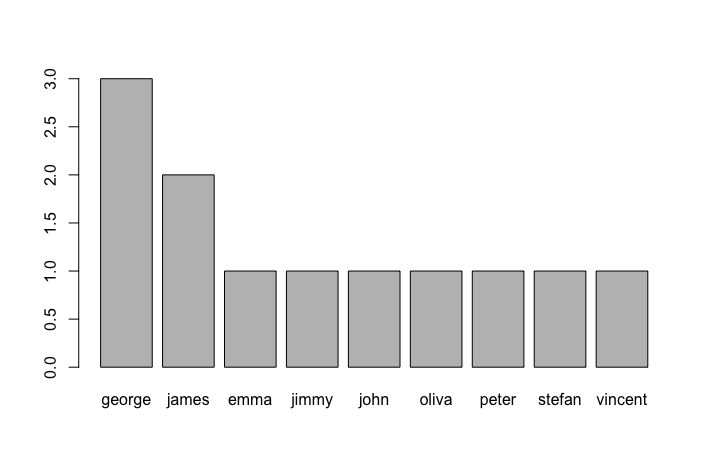
\includegraphics{name_freq.png}
\caption{Name frequency}\label{socialnetwork:fig-namefreq}\end{figure}
\begin{figure}[htbp]
\centering
\capstart

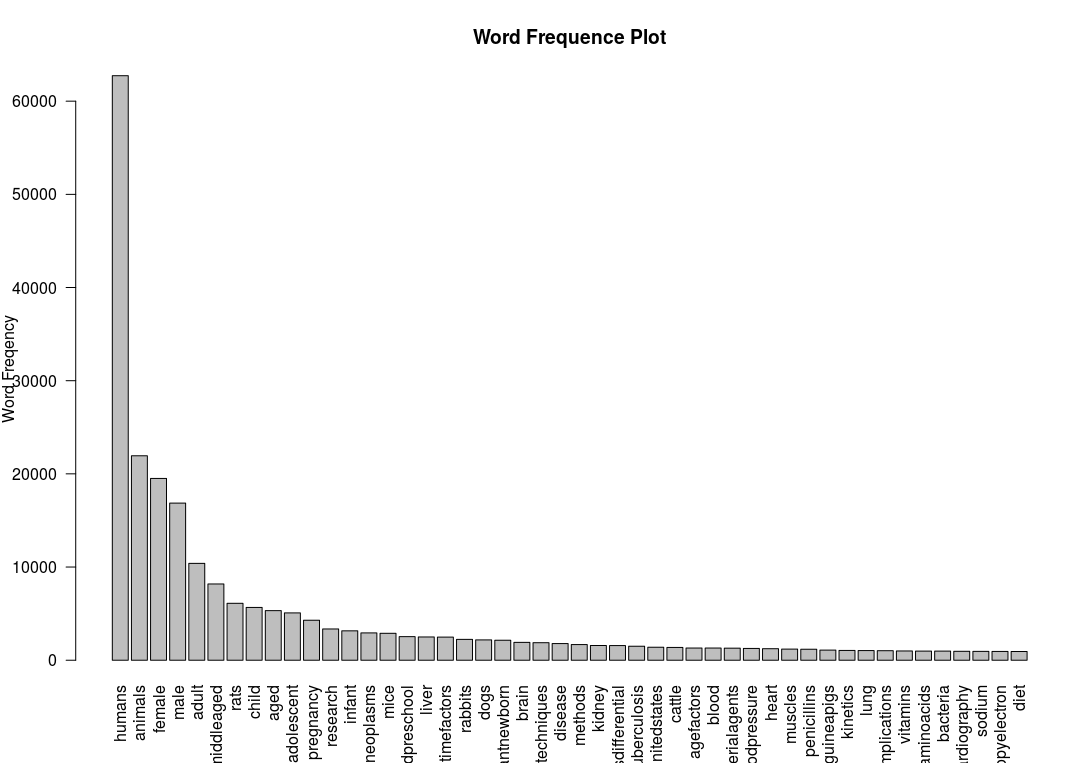
\includegraphics{word_freq.png}
\caption{Word frequency}\label{socialnetwork:fig-wordfreq}\end{figure}
\begin{figure}[htbp]
\centering
\capstart

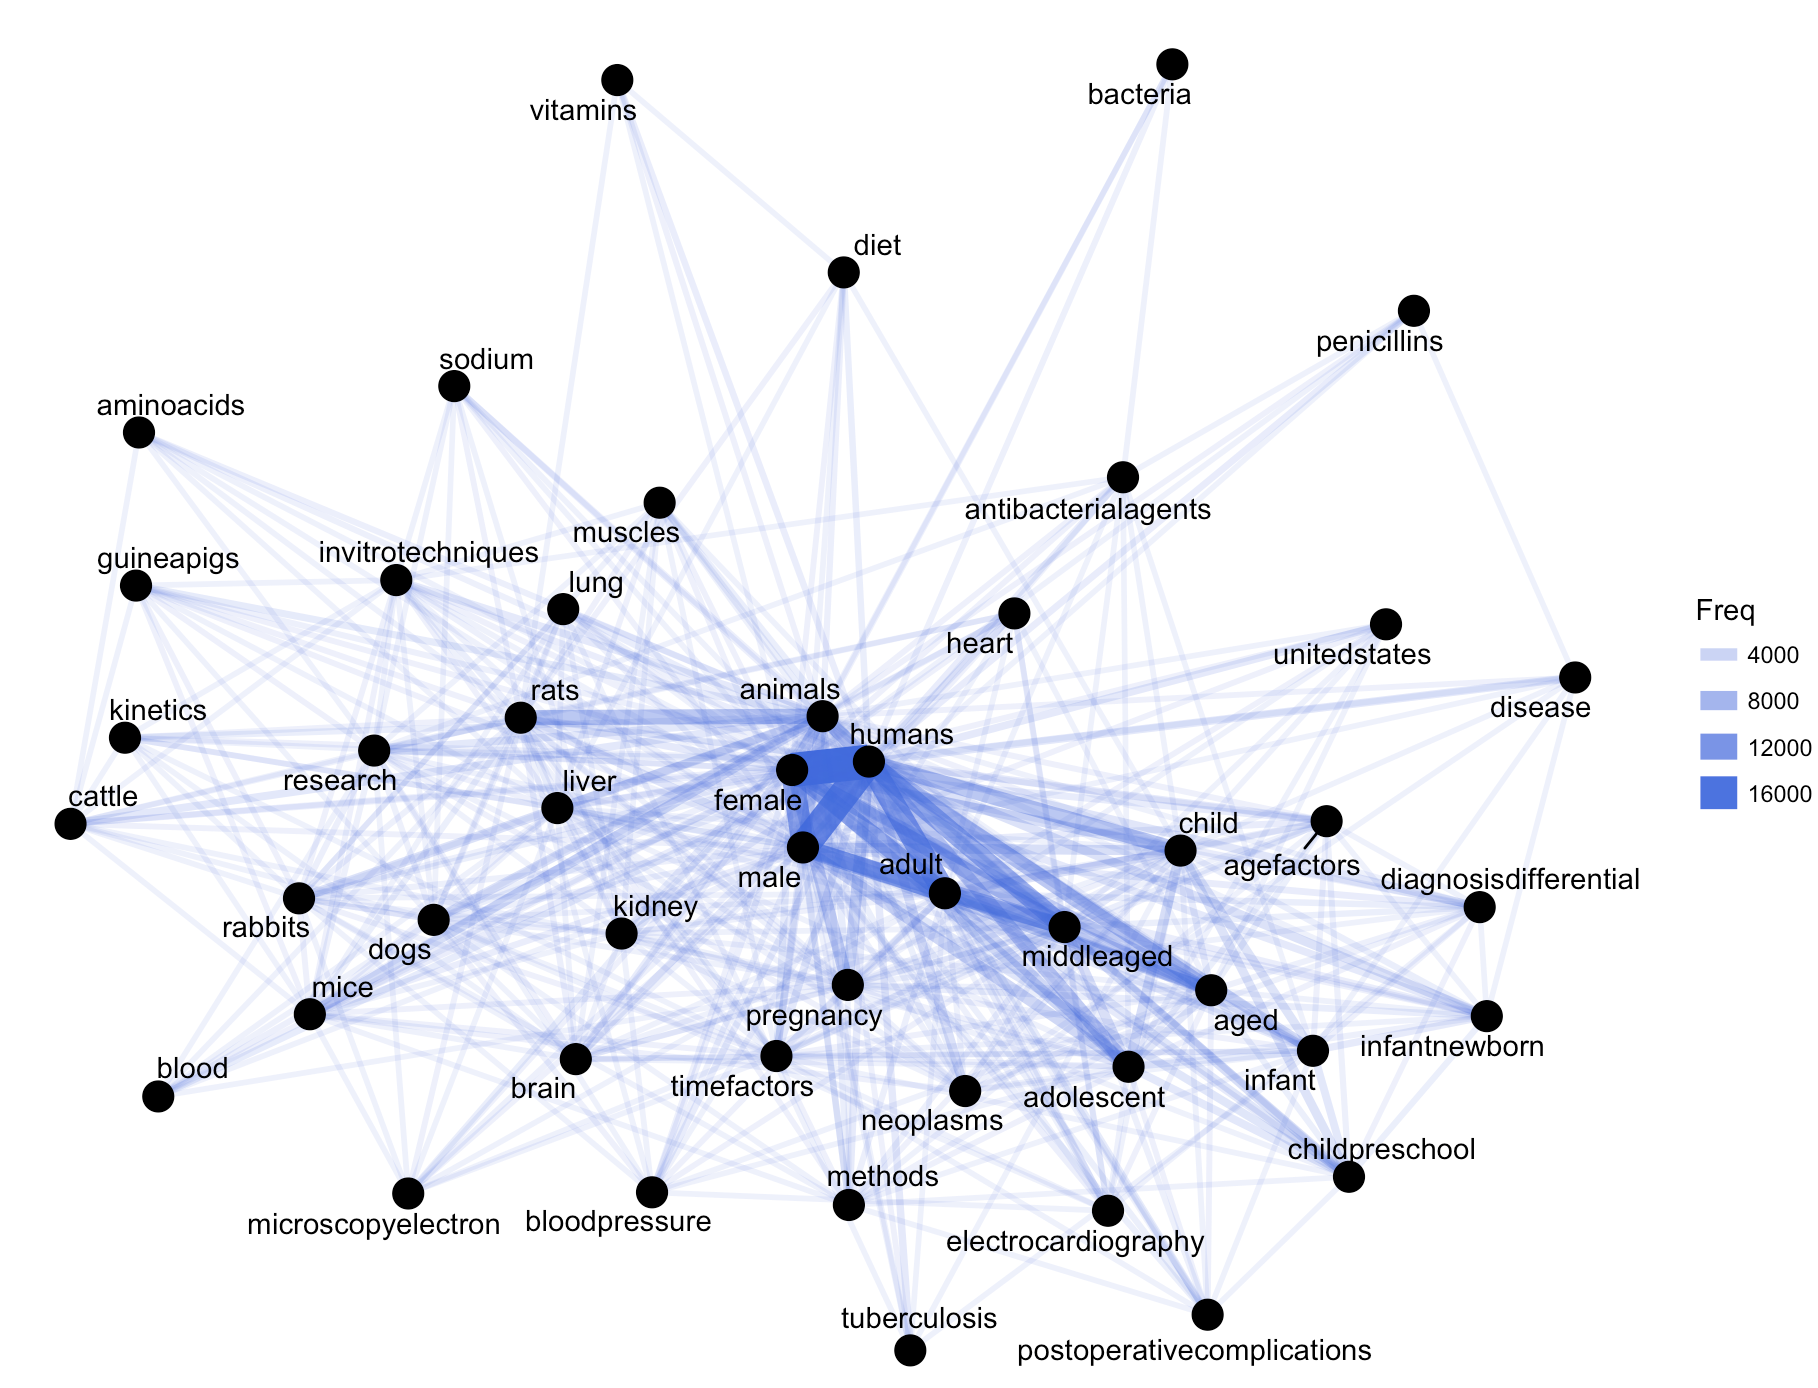
\includegraphics{netfreq.png}
\caption{Co-occurrence network}\label{socialnetwork:fig-netfreq}\end{figure}
\end{quote}

Then you will get Figure {\hyperref[socialnetwork:fig-netfreq]{\emph{Co-occurrence network}}}


\section{Correlation Network}
\label{socialnetwork:correlation-network}

\chapter{Neural Network}
\label{fnn:yassine-alouini}\label{fnn::doc}\label{fnn:neural-network}\label{fnn:fnn}
\begin{notice}{note}{Note:}
Sharpening the knife longer can make it easier to hack the firewood -- old Chinese proverb
\end{notice}


\section{Feedforward Neural Network}
\label{fnn:feedforward-neural-network}

\subsection{Introduction}
\label{fnn:introduction}
A feedforward neural network is an artificial neural network wherein connections between the units do not form a cycle. As such, it is different from recurrent neural networks.

The feedforward neural network was the first and simplest type of artificial neural network devised. In this network, the information moves in only one direction, forward (see Fig. {\hyperref[fnn:fig-fnn]{\emph{MultiLayer Neural Network}}}), from the input nodes, through the hidden nodes (if any) and to the output nodes. There are no cycles or loops in the network.
\begin{quote}
\begin{figure}[htbp]
\centering
\capstart

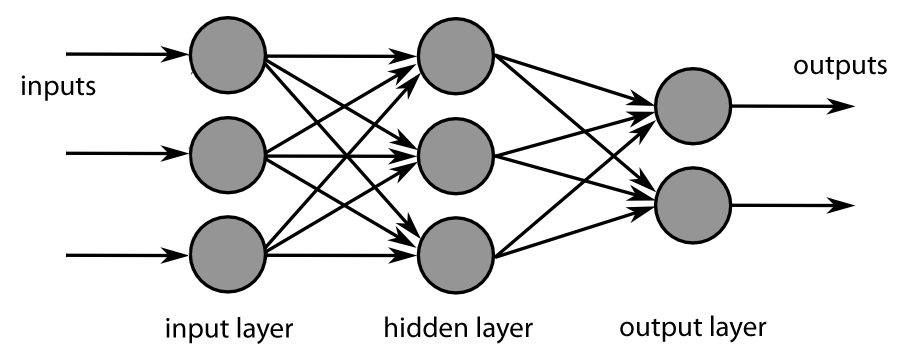
\includegraphics{fnn.png}
\caption{MultiLayer Neural Network}\label{fnn:fig-fnn}\end{figure}
\end{quote}


\subsection{Demo}
\label{fnn:demo}\begin{enumerate}
\item {} 
Set up spark context and SparkSession

\end{enumerate}

\begin{Verbatim}[commandchars=\\\{\}]
\PYG{k+kn}{from} \PYG{n+nn}{pyspark.sql} \PYG{k+kn}{import} \PYG{n}{SparkSession}

\PYG{n}{spark} \PYG{o}{=} \PYG{n}{SparkSession} \PYGZbs{}
    \PYG{o}{.}\PYG{n}{builder} \PYGZbs{}
    \PYG{o}{.}\PYG{n}{appName}\PYG{p}{(}\PYG{l+s}{\PYGZdq{}}\PYG{l+s}{Python Spark Feedforward neural network example}\PYG{l+s}{\PYGZdq{}}\PYG{p}{)} \PYGZbs{}
    \PYG{o}{.}\PYG{n}{config}\PYG{p}{(}\PYG{l+s}{\PYGZdq{}}\PYG{l+s}{spark.some.config.option}\PYG{l+s}{\PYGZdq{}}\PYG{p}{,} \PYG{l+s}{\PYGZdq{}}\PYG{l+s}{some\PYGZhy{}value}\PYG{l+s}{\PYGZdq{}}\PYG{p}{)} \PYGZbs{}
    \PYG{o}{.}\PYG{n}{getOrCreate}\PYG{p}{(}\PYG{p}{)}
\end{Verbatim}
\begin{enumerate}
\setcounter{enumi}{1}
\item {} 
Load dataset

\end{enumerate}

\begin{Verbatim}[commandchars=\\\{\}]
\PYG{o}{+}\PYG{o}{\PYGZhy{}}\PYG{o}{\PYGZhy{}}\PYG{o}{\PYGZhy{}}\PYG{o}{\PYGZhy{}}\PYG{o}{\PYGZhy{}}\PYG{o}{+}\PYG{o}{\PYGZhy{}}\PYG{o}{\PYGZhy{}}\PYG{o}{\PYGZhy{}}\PYG{o}{\PYGZhy{}}\PYG{o}{\PYGZhy{}}\PYG{o}{\PYGZhy{}}\PYG{o}{\PYGZhy{}}\PYG{o}{\PYGZhy{}}\PYG{o}{+}\PYG{o}{\PYGZhy{}}\PYG{o}{\PYGZhy{}}\PYG{o}{\PYGZhy{}}\PYG{o}{\PYGZhy{}}\PYG{o}{\PYGZhy{}}\PYG{o}{\PYGZhy{}}\PYG{o}{+}\PYG{o}{\PYGZhy{}}\PYG{o}{\PYGZhy{}}\PYG{o}{\PYGZhy{}}\PYG{o}{\PYGZhy{}}\PYG{o}{\PYGZhy{}}\PYG{o}{+}\PYG{o}{\PYGZhy{}}\PYG{o}{\PYGZhy{}}\PYG{o}{\PYGZhy{}}\PYG{o}{\PYGZhy{}}\PYG{o}{\PYGZhy{}}\PYG{o}{\PYGZhy{}}\PYG{o}{\PYGZhy{}}\PYG{o}{\PYGZhy{}}\PYG{o}{\PYGZhy{}}\PYG{o}{+}\PYG{o}{\PYGZhy{}}\PYG{o}{\PYGZhy{}}\PYG{o}{\PYGZhy{}}\PYG{o}{\PYGZhy{}}\PYG{o}{+}\PYG{o}{\PYGZhy{}}\PYG{o}{\PYGZhy{}}\PYG{o}{\PYGZhy{}}\PYG{o}{\PYGZhy{}}\PYG{o}{\PYGZhy{}}\PYG{o}{+}\PYG{o}{\PYGZhy{}}\PYG{o}{\PYGZhy{}}\PYG{o}{\PYGZhy{}}\PYG{o}{\PYGZhy{}}\PYG{o}{\PYGZhy{}}\PYG{o}{\PYGZhy{}}\PYG{o}{\PYGZhy{}}\PYG{o}{+}\PYG{o}{\PYGZhy{}}\PYG{o}{\PYGZhy{}}\PYG{o}{\PYGZhy{}}\PYG{o}{\PYGZhy{}}\PYG{o}{+}\PYG{o}{\PYGZhy{}}\PYG{o}{\PYGZhy{}}\PYG{o}{\PYGZhy{}}\PYG{o}{\PYGZhy{}}\PYG{o}{\PYGZhy{}}\PYG{o}{\PYGZhy{}}\PYG{o}{\PYGZhy{}}\PYG{o}{\PYGZhy{}}\PYG{o}{\PYGZhy{}}\PYG{o}{+}\PYG{o}{\PYGZhy{}}\PYG{o}{\PYGZhy{}}\PYG{o}{\PYGZhy{}}\PYG{o}{\PYGZhy{}}\PYG{o}{\PYGZhy{}}\PYG{o}{\PYGZhy{}}\PYG{o}{\PYGZhy{}}\PYG{o}{+}\PYG{o}{\PYGZhy{}}\PYG{o}{\PYGZhy{}}\PYG{o}{\PYGZhy{}}\PYG{o}{\PYGZhy{}}\PYG{o}{\PYGZhy{}}\PYG{o}{\PYGZhy{}}\PYG{o}{\PYGZhy{}}\PYG{o}{+}
\PYG{o}{\textbar{}}\PYG{n}{fixed}\PYG{o}{\textbar{}}\PYG{n}{volatile}\PYG{o}{\textbar{}}\PYG{n}{citric}\PYG{o}{\textbar{}}\PYG{n}{sugar}\PYG{o}{\textbar{}}\PYG{n}{chlorides}\PYG{o}{\textbar{}}\PYG{n}{free}\PYG{o}{\textbar{}}\PYG{n}{total}\PYG{o}{\textbar{}}\PYG{n}{density}\PYG{o}{\textbar{}}  \PYG{n}{pH}\PYG{o}{\textbar{}}\PYG{n}{sulphates}\PYG{o}{\textbar{}}\PYG{n}{alcohol}\PYG{o}{\textbar{}}\PYG{n}{quality}\PYG{o}{\textbar{}}
\PYG{o}{+}\PYG{o}{\PYGZhy{}}\PYG{o}{\PYGZhy{}}\PYG{o}{\PYGZhy{}}\PYG{o}{\PYGZhy{}}\PYG{o}{\PYGZhy{}}\PYG{o}{+}\PYG{o}{\PYGZhy{}}\PYG{o}{\PYGZhy{}}\PYG{o}{\PYGZhy{}}\PYG{o}{\PYGZhy{}}\PYG{o}{\PYGZhy{}}\PYG{o}{\PYGZhy{}}\PYG{o}{\PYGZhy{}}\PYG{o}{\PYGZhy{}}\PYG{o}{+}\PYG{o}{\PYGZhy{}}\PYG{o}{\PYGZhy{}}\PYG{o}{\PYGZhy{}}\PYG{o}{\PYGZhy{}}\PYG{o}{\PYGZhy{}}\PYG{o}{\PYGZhy{}}\PYG{o}{+}\PYG{o}{\PYGZhy{}}\PYG{o}{\PYGZhy{}}\PYG{o}{\PYGZhy{}}\PYG{o}{\PYGZhy{}}\PYG{o}{\PYGZhy{}}\PYG{o}{+}\PYG{o}{\PYGZhy{}}\PYG{o}{\PYGZhy{}}\PYG{o}{\PYGZhy{}}\PYG{o}{\PYGZhy{}}\PYG{o}{\PYGZhy{}}\PYG{o}{\PYGZhy{}}\PYG{o}{\PYGZhy{}}\PYG{o}{\PYGZhy{}}\PYG{o}{\PYGZhy{}}\PYG{o}{+}\PYG{o}{\PYGZhy{}}\PYG{o}{\PYGZhy{}}\PYG{o}{\PYGZhy{}}\PYG{o}{\PYGZhy{}}\PYG{o}{+}\PYG{o}{\PYGZhy{}}\PYG{o}{\PYGZhy{}}\PYG{o}{\PYGZhy{}}\PYG{o}{\PYGZhy{}}\PYG{o}{\PYGZhy{}}\PYG{o}{+}\PYG{o}{\PYGZhy{}}\PYG{o}{\PYGZhy{}}\PYG{o}{\PYGZhy{}}\PYG{o}{\PYGZhy{}}\PYG{o}{\PYGZhy{}}\PYG{o}{\PYGZhy{}}\PYG{o}{\PYGZhy{}}\PYG{o}{+}\PYG{o}{\PYGZhy{}}\PYG{o}{\PYGZhy{}}\PYG{o}{\PYGZhy{}}\PYG{o}{\PYGZhy{}}\PYG{o}{+}\PYG{o}{\PYGZhy{}}\PYG{o}{\PYGZhy{}}\PYG{o}{\PYGZhy{}}\PYG{o}{\PYGZhy{}}\PYG{o}{\PYGZhy{}}\PYG{o}{\PYGZhy{}}\PYG{o}{\PYGZhy{}}\PYG{o}{\PYGZhy{}}\PYG{o}{\PYGZhy{}}\PYG{o}{+}\PYG{o}{\PYGZhy{}}\PYG{o}{\PYGZhy{}}\PYG{o}{\PYGZhy{}}\PYG{o}{\PYGZhy{}}\PYG{o}{\PYGZhy{}}\PYG{o}{\PYGZhy{}}\PYG{o}{\PYGZhy{}}\PYG{o}{+}\PYG{o}{\PYGZhy{}}\PYG{o}{\PYGZhy{}}\PYG{o}{\PYGZhy{}}\PYG{o}{\PYGZhy{}}\PYG{o}{\PYGZhy{}}\PYG{o}{\PYGZhy{}}\PYG{o}{\PYGZhy{}}\PYG{o}{+}
\PYG{o}{\textbar{}}  \PYG{l+m+mf}{7.4}\PYG{o}{\textbar{}}     \PYG{l+m+mf}{0.7}\PYG{o}{\textbar{}}   \PYG{l+m+mf}{0.0}\PYG{o}{\textbar{}}  \PYG{l+m+mf}{1.9}\PYG{o}{\textbar{}}    \PYG{l+m+mf}{0.076}\PYG{o}{\textbar{}}\PYG{l+m+mf}{11.0}\PYG{o}{\textbar{}} \PYG{l+m+mf}{34.0}\PYG{o}{\textbar{}} \PYG{l+m+mf}{0.9978}\PYG{o}{\textbar{}}\PYG{l+m+mf}{3.51}\PYG{o}{\textbar{}}     \PYG{l+m+mf}{0.56}\PYG{o}{\textbar{}}    \PYG{l+m+mf}{9.4}\PYG{o}{\textbar{}}      \PYG{l+m+mi}{5}\PYG{o}{\textbar{}}
\PYG{o}{\textbar{}}  \PYG{l+m+mf}{7.8}\PYG{o}{\textbar{}}    \PYG{l+m+mf}{0.88}\PYG{o}{\textbar{}}   \PYG{l+m+mf}{0.0}\PYG{o}{\textbar{}}  \PYG{l+m+mf}{2.6}\PYG{o}{\textbar{}}    \PYG{l+m+mf}{0.098}\PYG{o}{\textbar{}}\PYG{l+m+mf}{25.0}\PYG{o}{\textbar{}} \PYG{l+m+mf}{67.0}\PYG{o}{\textbar{}} \PYG{l+m+mf}{0.9968}\PYG{o}{\textbar{}} \PYG{l+m+mf}{3.2}\PYG{o}{\textbar{}}     \PYG{l+m+mf}{0.68}\PYG{o}{\textbar{}}    \PYG{l+m+mf}{9.8}\PYG{o}{\textbar{}}      \PYG{l+m+mi}{5}\PYG{o}{\textbar{}}
\PYG{o}{\textbar{}}  \PYG{l+m+mf}{7.8}\PYG{o}{\textbar{}}    \PYG{l+m+mf}{0.76}\PYG{o}{\textbar{}}  \PYG{l+m+mf}{0.04}\PYG{o}{\textbar{}}  \PYG{l+m+mf}{2.3}\PYG{o}{\textbar{}}    \PYG{l+m+mf}{0.092}\PYG{o}{\textbar{}}\PYG{l+m+mf}{15.0}\PYG{o}{\textbar{}} \PYG{l+m+mf}{54.0}\PYG{o}{\textbar{}}  \PYG{l+m+mf}{0.997}\PYG{o}{\textbar{}}\PYG{l+m+mf}{3.26}\PYG{o}{\textbar{}}     \PYG{l+m+mf}{0.65}\PYG{o}{\textbar{}}    \PYG{l+m+mf}{9.8}\PYG{o}{\textbar{}}      \PYG{l+m+mi}{5}\PYG{o}{\textbar{}}
\PYG{o}{\textbar{}} \PYG{l+m+mf}{11.2}\PYG{o}{\textbar{}}    \PYG{l+m+mf}{0.28}\PYG{o}{\textbar{}}  \PYG{l+m+mf}{0.56}\PYG{o}{\textbar{}}  \PYG{l+m+mf}{1.9}\PYG{o}{\textbar{}}    \PYG{l+m+mf}{0.075}\PYG{o}{\textbar{}}\PYG{l+m+mf}{17.0}\PYG{o}{\textbar{}} \PYG{l+m+mf}{60.0}\PYG{o}{\textbar{}}  \PYG{l+m+mf}{0.998}\PYG{o}{\textbar{}}\PYG{l+m+mf}{3.16}\PYG{o}{\textbar{}}     \PYG{l+m+mf}{0.58}\PYG{o}{\textbar{}}    \PYG{l+m+mf}{9.8}\PYG{o}{\textbar{}}      \PYG{l+m+mi}{6}\PYG{o}{\textbar{}}
\PYG{o}{\textbar{}}  \PYG{l+m+mf}{7.4}\PYG{o}{\textbar{}}     \PYG{l+m+mf}{0.7}\PYG{o}{\textbar{}}   \PYG{l+m+mf}{0.0}\PYG{o}{\textbar{}}  \PYG{l+m+mf}{1.9}\PYG{o}{\textbar{}}    \PYG{l+m+mf}{0.076}\PYG{o}{\textbar{}}\PYG{l+m+mf}{11.0}\PYG{o}{\textbar{}} \PYG{l+m+mf}{34.0}\PYG{o}{\textbar{}} \PYG{l+m+mf}{0.9978}\PYG{o}{\textbar{}}\PYG{l+m+mf}{3.51}\PYG{o}{\textbar{}}     \PYG{l+m+mf}{0.56}\PYG{o}{\textbar{}}    \PYG{l+m+mf}{9.4}\PYG{o}{\textbar{}}      \PYG{l+m+mi}{5}\PYG{o}{\textbar{}}
\PYG{o}{+}\PYG{o}{\PYGZhy{}}\PYG{o}{\PYGZhy{}}\PYG{o}{\PYGZhy{}}\PYG{o}{\PYGZhy{}}\PYG{o}{\PYGZhy{}}\PYG{o}{+}\PYG{o}{\PYGZhy{}}\PYG{o}{\PYGZhy{}}\PYG{o}{\PYGZhy{}}\PYG{o}{\PYGZhy{}}\PYG{o}{\PYGZhy{}}\PYG{o}{\PYGZhy{}}\PYG{o}{\PYGZhy{}}\PYG{o}{\PYGZhy{}}\PYG{o}{+}\PYG{o}{\PYGZhy{}}\PYG{o}{\PYGZhy{}}\PYG{o}{\PYGZhy{}}\PYG{o}{\PYGZhy{}}\PYG{o}{\PYGZhy{}}\PYG{o}{\PYGZhy{}}\PYG{o}{+}\PYG{o}{\PYGZhy{}}\PYG{o}{\PYGZhy{}}\PYG{o}{\PYGZhy{}}\PYG{o}{\PYGZhy{}}\PYG{o}{\PYGZhy{}}\PYG{o}{+}\PYG{o}{\PYGZhy{}}\PYG{o}{\PYGZhy{}}\PYG{o}{\PYGZhy{}}\PYG{o}{\PYGZhy{}}\PYG{o}{\PYGZhy{}}\PYG{o}{\PYGZhy{}}\PYG{o}{\PYGZhy{}}\PYG{o}{\PYGZhy{}}\PYG{o}{\PYGZhy{}}\PYG{o}{+}\PYG{o}{\PYGZhy{}}\PYG{o}{\PYGZhy{}}\PYG{o}{\PYGZhy{}}\PYG{o}{\PYGZhy{}}\PYG{o}{+}\PYG{o}{\PYGZhy{}}\PYG{o}{\PYGZhy{}}\PYG{o}{\PYGZhy{}}\PYG{o}{\PYGZhy{}}\PYG{o}{\PYGZhy{}}\PYG{o}{+}\PYG{o}{\PYGZhy{}}\PYG{o}{\PYGZhy{}}\PYG{o}{\PYGZhy{}}\PYG{o}{\PYGZhy{}}\PYG{o}{\PYGZhy{}}\PYG{o}{\PYGZhy{}}\PYG{o}{\PYGZhy{}}\PYG{o}{+}\PYG{o}{\PYGZhy{}}\PYG{o}{\PYGZhy{}}\PYG{o}{\PYGZhy{}}\PYG{o}{\PYGZhy{}}\PYG{o}{+}\PYG{o}{\PYGZhy{}}\PYG{o}{\PYGZhy{}}\PYG{o}{\PYGZhy{}}\PYG{o}{\PYGZhy{}}\PYG{o}{\PYGZhy{}}\PYG{o}{\PYGZhy{}}\PYG{o}{\PYGZhy{}}\PYG{o}{\PYGZhy{}}\PYG{o}{\PYGZhy{}}\PYG{o}{+}\PYG{o}{\PYGZhy{}}\PYG{o}{\PYGZhy{}}\PYG{o}{\PYGZhy{}}\PYG{o}{\PYGZhy{}}\PYG{o}{\PYGZhy{}}\PYG{o}{\PYGZhy{}}\PYG{o}{\PYGZhy{}}\PYG{o}{+}\PYG{o}{\PYGZhy{}}\PYG{o}{\PYGZhy{}}\PYG{o}{\PYGZhy{}}\PYG{o}{\PYGZhy{}}\PYG{o}{\PYGZhy{}}\PYG{o}{\PYGZhy{}}\PYG{o}{\PYGZhy{}}\PYG{o}{+}
\PYG{n}{only} \PYG{n}{showing} \PYG{n}{top} \PYG{l+m+mi}{5} \PYG{n}{rows}
\end{Verbatim}
\begin{enumerate}
\setcounter{enumi}{2}
\item {} 
change categorical variable size

\end{enumerate}

\begin{Verbatim}[commandchars=\\\{\}]
\PYG{c}{\PYGZsh{} Convert to float format}
\PYG{k}{def} \PYG{n+nf}{string\PYGZus{}to\PYGZus{}float}\PYG{p}{(}\PYG{n}{x}\PYG{p}{)}\PYG{p}{:}
    \PYG{k}{return} \PYG{n+nb}{float}\PYG{p}{(}\PYG{n}{x}\PYG{p}{)}

\PYG{c}{\PYGZsh{}}
\PYG{k}{def} \PYG{n+nf}{condition}\PYG{p}{(}\PYG{n}{r}\PYG{p}{)}\PYG{p}{:}
    \PYG{k}{if} \PYG{p}{(}\PYG{l+m+mi}{0}\PYG{o}{\PYGZlt{}}\PYG{o}{=} \PYG{n}{r} \PYG{o}{\PYGZlt{}}\PYG{o}{=} \PYG{l+m+mi}{4}\PYG{p}{)}\PYG{p}{:}
        \PYG{n}{label} \PYG{o}{=} \PYG{l+s}{\PYGZdq{}}\PYG{l+s}{low}\PYG{l+s}{\PYGZdq{}}
    \PYG{k}{elif}\PYG{p}{(}\PYG{l+m+mi}{4}\PYG{o}{\PYGZlt{}} \PYG{n}{r} \PYG{o}{\PYGZlt{}}\PYG{o}{=} \PYG{l+m+mi}{6}\PYG{p}{)}\PYG{p}{:}
        \PYG{n}{label} \PYG{o}{=} \PYG{l+s}{\PYGZdq{}}\PYG{l+s}{medium}\PYG{l+s}{\PYGZdq{}}
    \PYG{k}{else}\PYG{p}{:}
        \PYG{n}{label} \PYG{o}{=} \PYG{l+s}{\PYGZdq{}}\PYG{l+s}{high}\PYG{l+s}{\PYGZdq{}}
    \PYG{k}{return} \PYG{n}{label}
\end{Verbatim}

\begin{Verbatim}[commandchars=\\\{\}]
\PYG{k+kn}{from} \PYG{n+nn}{pyspark.sql.functions} \PYG{k+kn}{import} \PYG{n}{udf}
\PYG{k+kn}{from} \PYG{n+nn}{pyspark.sql.types} \PYG{k+kn}{import} \PYG{n}{StringType}\PYG{p}{,} \PYG{n}{DoubleType}
\PYG{n}{string\PYGZus{}to\PYGZus{}float\PYGZus{}udf} \PYG{o}{=} \PYG{n}{udf}\PYG{p}{(}\PYG{n}{string\PYGZus{}to\PYGZus{}float}\PYG{p}{,} \PYG{n}{DoubleType}\PYG{p}{(}\PYG{p}{)}\PYG{p}{)}
\PYG{n}{quality\PYGZus{}udf} \PYG{o}{=} \PYG{n}{udf}\PYG{p}{(}\PYG{k}{lambda} \PYG{n}{x}\PYG{p}{:} \PYG{n}{condition}\PYG{p}{(}\PYG{n}{x}\PYG{p}{)}\PYG{p}{,} \PYG{n}{StringType}\PYG{p}{(}\PYG{p}{)}\PYG{p}{)}
\PYG{n}{df}\PYG{o}{=} \PYG{n}{df}\PYG{o}{.}\PYG{n}{withColumn}\PYG{p}{(}\PYG{l+s}{\PYGZdq{}}\PYG{l+s}{quality}\PYG{l+s}{\PYGZdq{}}\PYG{p}{,} \PYG{n}{quality\PYGZus{}udf}\PYG{p}{(}\PYG{l+s}{\PYGZdq{}}\PYG{l+s}{quality}\PYG{l+s}{\PYGZdq{}}\PYG{p}{)}\PYG{p}{)}
\end{Verbatim}
\begin{enumerate}
\setcounter{enumi}{3}
\item {} 
Convert the data to dense vector

\end{enumerate}

\begin{Verbatim}[commandchars=\\\{\}]
\PYG{c}{\PYGZsh{} convert the data to dense vector}
\PYG{k}{def} \PYG{n+nf}{transData}\PYG{p}{(}\PYG{n}{data}\PYG{p}{)}\PYG{p}{:}
    \PYG{k}{return} \PYG{n}{data}\PYG{o}{.}\PYG{n}{rdd}\PYG{o}{.}\PYG{n}{map}\PYG{p}{(}\PYG{k}{lambda} \PYG{n}{r}\PYG{p}{:} \PYG{p}{[}\PYG{n}{r}\PYG{p}{[}\PYG{o}{\PYGZhy{}}\PYG{l+m+mi}{1}\PYG{p}{]}\PYG{p}{,} \PYG{n}{Vectors}\PYG{o}{.}\PYG{n}{dense}\PYG{p}{(}\PYG{n}{r}\PYG{p}{[}\PYG{p}{:}\PYG{o}{\PYGZhy{}}\PYG{l+m+mi}{1}\PYG{p}{]}\PYG{p}{)}\PYG{p}{]}\PYG{p}{)}\PYG{o}{.}\PYGZbs{}
           \PYG{n}{toDF}\PYG{p}{(}\PYG{p}{[}\PYG{l+s}{\PYGZsq{}}\PYG{l+s}{label}\PYG{l+s}{\PYGZsq{}}\PYG{p}{,}\PYG{l+s}{\PYGZsq{}}\PYG{l+s}{features}\PYG{l+s}{\PYGZsq{}}\PYG{p}{]}\PYG{p}{)}

\PYG{k+kn}{from} \PYG{n+nn}{pyspark.sql} \PYG{k+kn}{import} \PYG{n}{Row}
\PYG{k+kn}{from} \PYG{n+nn}{pyspark.ml.linalg} \PYG{k+kn}{import} \PYG{n}{Vectors}

\PYG{n}{data}\PYG{o}{=} \PYG{n}{transData}\PYG{p}{(}\PYG{n}{df}\PYG{p}{)}
\PYG{n}{data}\PYG{o}{.}\PYG{n}{show}\PYG{p}{(}\PYG{p}{)}
\end{Verbatim}
\begin{enumerate}
\setcounter{enumi}{4}
\item {} 
Split the data into training and test sets (40\% held out for testing)

\end{enumerate}

\begin{Verbatim}[commandchars=\\\{\}]
\PYG{c}{\PYGZsh{} Split the data into train and test}
\PYG{p}{(}\PYG{n}{trainingData}\PYG{p}{,} \PYG{n}{testData}\PYG{p}{)} \PYG{o}{=} \PYG{n}{data}\PYG{o}{.}\PYG{n}{randomSplit}\PYG{p}{(}\PYG{p}{[}\PYG{l+m+mf}{0.6}\PYG{p}{,} \PYG{l+m+mf}{0.4}\PYG{p}{]}\PYG{p}{)}
\end{Verbatim}
\begin{enumerate}
\setcounter{enumi}{5}
\item {} 
Train neural network

\end{enumerate}

\begin{Verbatim}[commandchars=\\\{\}]
\PYG{c}{\PYGZsh{} specify layers for the neural network:}
\PYG{c}{\PYGZsh{} input layer of size 11 (features), two intermediate of size 5 and 4}
\PYG{c}{\PYGZsh{} and output of size 7 (classes)}
\PYG{n}{layers} \PYG{o}{=} \PYG{p}{[}\PYG{l+m+mi}{11}\PYG{p}{,} \PYG{l+m+mi}{5}\PYG{p}{,} \PYG{l+m+mi}{4}\PYG{p}{,} \PYG{l+m+mi}{4}\PYG{p}{,} \PYG{l+m+mi}{3} \PYG{p}{,} \PYG{l+m+mi}{7}\PYG{p}{]}

\PYG{c}{\PYGZsh{} create the trainer and set its parameters}
\PYG{n}{FNN} \PYG{o}{=} \PYG{n}{MultilayerPerceptronClassifier}\PYG{p}{(}\PYG{n}{labelCol}\PYG{o}{=}\PYG{l+s}{\PYGZdq{}}\PYG{l+s}{indexedLabel}\PYG{l+s}{\PYGZdq{}}\PYG{p}{,} \PYGZbs{}
                                     \PYG{n}{featuresCol}\PYG{o}{=}\PYG{l+s}{\PYGZdq{}}\PYG{l+s}{indexedFeatures}\PYG{l+s}{\PYGZdq{}}\PYG{p}{,}\PYGZbs{}
                                     \PYG{n}{maxIter}\PYG{o}{=}\PYG{l+m+mi}{100}\PYG{p}{,} \PYG{n}{layers}\PYG{o}{=}\PYG{n}{layers}\PYG{p}{,} \PYGZbs{}
                                     \PYG{n}{blockSize}\PYG{o}{=}\PYG{l+m+mi}{128}\PYG{p}{,} \PYG{n}{seed}\PYG{o}{=}\PYG{l+m+mi}{1234}\PYG{p}{)}
\PYG{c}{\PYGZsh{} Convert indexed labels back to original labels.}
\PYG{n}{labelConverter} \PYG{o}{=} \PYG{n}{IndexToString}\PYG{p}{(}\PYG{n}{inputCol}\PYG{o}{=}\PYG{l+s}{\PYGZdq{}}\PYG{l+s}{prediction}\PYG{l+s}{\PYGZdq{}}\PYG{p}{,} \PYG{n}{outputCol}\PYG{o}{=}\PYG{l+s}{\PYGZdq{}}\PYG{l+s}{predictedLabel}\PYG{l+s}{\PYGZdq{}}\PYG{p}{,}
                               \PYG{n}{labels}\PYG{o}{=}\PYG{n}{labelIndexer}\PYG{o}{.}\PYG{n}{labels}\PYG{p}{)}
\PYG{c}{\PYGZsh{} Chain indexers and forest in a Pipeline}
\PYG{k+kn}{from} \PYG{n+nn}{pyspark.ml} \PYG{k+kn}{import} \PYG{n}{Pipeline}
\PYG{n}{pipeline} \PYG{o}{=} \PYG{n}{Pipeline}\PYG{p}{(}\PYG{n}{stages}\PYG{o}{=}\PYG{p}{[}\PYG{n}{labelIndexer}\PYG{p}{,} \PYG{n}{featureIndexer}\PYG{p}{,} \PYG{n}{FNN}\PYG{p}{,} \PYG{n}{labelConverter}\PYG{p}{]}\PYG{p}{)}
\PYG{c}{\PYGZsh{} train the model}
\PYG{c}{\PYGZsh{} Train model.  This also runs the indexers.}
\PYG{n}{model} \PYG{o}{=} \PYG{n}{pipeline}\PYG{o}{.}\PYG{n}{fit}\PYG{p}{(}\PYG{n}{trainingData}\PYG{p}{)}
\end{Verbatim}
\begin{enumerate}
\setcounter{enumi}{6}
\item {} 
Make predictions

\end{enumerate}

\begin{Verbatim}[commandchars=\\\{\}]
\PYG{c}{\PYGZsh{} Make predictions.}
\PYG{n}{predictions} \PYG{o}{=} \PYG{n}{model}\PYG{o}{.}\PYG{n}{transform}\PYG{p}{(}\PYG{n}{testData}\PYG{p}{)}
\PYG{c}{\PYGZsh{} Select example rows to display.}
\PYG{n}{predictions}\PYG{o}{.}\PYG{n}{select}\PYG{p}{(}\PYG{l+s}{\PYGZdq{}}\PYG{l+s}{features}\PYG{l+s}{\PYGZdq{}}\PYG{p}{,}\PYG{l+s}{\PYGZdq{}}\PYG{l+s}{label}\PYG{l+s}{\PYGZdq{}}\PYG{p}{,}\PYG{l+s}{\PYGZdq{}}\PYG{l+s}{predictedLabel}\PYG{l+s}{\PYGZdq{}}\PYG{p}{)}\PYG{o}{.}\PYG{n}{show}\PYG{p}{(}\PYG{l+m+mi}{5}\PYG{p}{)}
\end{Verbatim}
\begin{enumerate}
\setcounter{enumi}{7}
\item {} 
Evaluation

\end{enumerate}

\begin{Verbatim}[commandchars=\\\{\}]
\PYG{c}{\PYGZsh{} Select (prediction, true label) and compute test error}
\PYG{n}{evaluator} \PYG{o}{=} \PYG{n}{MulticlassClassificationEvaluator}\PYG{p}{(}
    \PYG{n}{labelCol}\PYG{o}{=}\PYG{l+s}{\PYGZdq{}}\PYG{l+s}{indexedLabel}\PYG{l+s}{\PYGZdq{}}\PYG{p}{,} \PYG{n}{predictionCol}\PYG{o}{=}\PYG{l+s}{\PYGZdq{}}\PYG{l+s}{prediction}\PYG{l+s}{\PYGZdq{}}\PYG{p}{,} \PYG{n}{metricName}\PYG{o}{=}\PYG{l+s}{\PYGZdq{}}\PYG{l+s}{accuracy}\PYG{l+s}{\PYGZdq{}}\PYG{p}{)}
\PYG{n}{accuracy} \PYG{o}{=} \PYG{n}{evaluator}\PYG{o}{.}\PYG{n}{evaluate}\PYG{p}{(}\PYG{n}{predictions}\PYG{p}{)}
\PYG{k}{print}\PYG{p}{(}\PYG{l+s}{\PYGZdq{}}\PYG{l+s}{Predictions accuracy = }\PYG{l+s+si}{\PYGZpc{}g}\PYG{l+s}{, Test Error = }\PYG{l+s+si}{\PYGZpc{}g}\PYG{l+s}{\PYGZdq{}} \PYG{o}{\PYGZpc{}} \PYG{p}{(}\PYG{n}{accuracy}\PYG{p}{,}\PYG{p}{(}\PYG{l+m+mf}{1.0} \PYG{o}{\PYGZhy{}} \PYG{n}{accuracy}\PYG{p}{)}\PYG{p}{)}\PYG{p}{)}
\end{Verbatim}


\chapter{Main Reference}
\label{reference:yassine-alouini}\label{reference::doc}\label{reference:reference}\label{reference:main-reference}
\begin{thebibliography}{Kirillov2016}
\bibitem[Bird2009]{Bird2009}{\phantomsection\label{reference:bird2009} \begin{enumerate}
\setcounter{enumi}{18}
\item {} 
Bird, E. Klein, and E. Loper. Natural language processing with Python: analyzing text with the natural language toolkit. O’Reilly Media, Inc., 2009.

\end{enumerate}
}
\bibitem[Feng2017]{Feng2017}{\phantomsection\label{reference:feng2017} \begin{enumerate}
\setcounter{enumi}{22}
\item {} 
Feng and M. Chen. \href{https://mingchen0919.github.io/learning-apache-spark/index.html}{Learning Apache Spark}, Github 2017.

\end{enumerate}
}
\bibitem[Karau2015]{Karau2015}{\phantomsection\label{reference:karau2015} \begin{enumerate}
\setcounter{enumi}{7}
\item {} 
Karau, A. Konwinski, P. Wendell and M. Zaharia. Learning Spark: Lightning-Fast Big Data Analysis. O’Reilly Media, Inc., 2015

\end{enumerate}
}
\bibitem[Kirillov2016]{Kirillov2016}{\phantomsection\label{reference:kirillov2016} 
Anton Kirillov. Apache Spark: core concepts, architecture and internals. \href{http://datastrophic.io/core-concepts-architecture-and-internals-of-apache-spark/}{http://datastrophic.io/core-concepts-architecture-and-internals-of-apache-spark/}
}
\end{thebibliography}



\renewcommand{\indexname}{Index}
\printindex
\end{document}
